% LaTeX Template for GenSoftworks Documents (GDD, WBB)
% A4 Portrait, Normal Document Layout
% XeLaTeX required
% Fonts from assets/fonts/

\documentclass[10pt, a4paper, oneside]{article}

% ==========================================================================
%   PACKAGES & FONTS
% ==========================================================================

\usepackage{fontspec}

\def\fontpath{/Users/jennifer/Documents/GitHub/gensoftworks/assets/fonts/}

% Body: Open Sans 10pt
\setmainfont{OpenSans}[
  Path = \fontpath,
  UprightFont = {OpenSans-Variable.ttf},
  ItalicFont = {OpenSans-Italic-Variable.ttf},
  BoldFont = {OpenSans-Variable.ttf},
  BoldItalicFont = {OpenSans-Italic-Variable.ttf},
  BoldFeatures = {Weight=700},
  BoldItalicFeatures = {Weight=700}
]

\setsansfont{OpenSans}[
  Path = \fontpath,
  UprightFont = {OpenSans-Variable.ttf},
  ItalicFont = {OpenSans-Italic-Variable.ttf},
  BoldFont = {OpenSans-Variable.ttf},
  BoldItalicFont = {OpenSans-Italic-Variable.ttf},
  BoldFeatures = {Weight=700},
  BoldItalicFeatures = {Weight=700}
]

\setmonofont{JetBrainsMono}[
  Path = \fontpath,
  UprightFont = {JetBrainsMono-Variable.ttf},
  ItalicFont = {JetBrainsMono-Italic-Variable.ttf},
  BoldFont = {JetBrainsMono-Variable.ttf},
  BoldItalicFont = {JetBrainsMono-Italic-Variable.ttf},
  BoldFeatures = {Weight=700},
  BoldItalicFeatures = {Weight=700},
  Scale = 0.85
]

% Heading font: Source Serif 4 Italic
\newfontfamily\headingfont{SourceSerif4}[
  Path = \fontpath,
  UprightFont = {SourceSerif4-Variable.ttf},
  ItalicFont = {SourceSerif4-Italic-Variable.ttf},
  BoldFont = {SourceSerif4-Variable.ttf},
  BoldItalicFont = {SourceSerif4-Italic-Variable.ttf},
  BoldFeatures = {Weight=700},
  BoldItalicFeatures = {Weight=700}
]

\let\titlefont\headingfont

\usepackage{polyglossia}
\setdefaultlanguage{german}

% Page layout
\usepackage[a4paper, left=25mm, right=25mm, top=25mm, bottom=25mm]{geometry}

% Colors
\usepackage{xcolor}
\definecolor{black}{HTML}{1A1A1A}
\definecolor{gray}{HTML}{888888}
\definecolor{lightgray}{HTML}{BBBBBB}
\definecolor{border}{HTML}{DDDDDD}
\definecolor{boxbg}{HTML}{F5F5F5}
\definecolor{quotetint}{HTML}{F0F0F0}
\definecolor{scenelabel}{HTML}{666666}

% ==========================================================================
%   SPACING — normal document (not compressed like logbook)
% ==========================================================================

\usepackage{setspace}
\setstretch{1.4}
\setlength{\parindent}{0pt}
\setlength{\parskip}{4pt plus 1pt minus 1pt}

% ==========================================================================
%   HEADINGS
% ==========================================================================

\usepackage{fancyhdr}
\pagestyle{fancy}
\fancyhf{}
\renewcommand{\headrulewidth}{0pt}
\fancyfoot[C]{\small\color{gray}\thepage}
\fancyhead[R]{\small\color{lightgray}\itshape GDD}
\fancypagestyle{plain}{\fancyhf{}\renewcommand{\headrulewidth}{0pt}}

\usepackage{titlesec}
\setcounter{secnumdepth}{0}
\setcounter{tocdepth}{3}

% H1 — Chapter
\titleformat{\section}
  {\headingfont\fontsize{22pt}{26pt}\selectfont\itshape\color{black}}
  {}{0em}{}
\titlespacing*{\section}{0pt}{8mm}{4mm}

\newcommand{\sectionbreak}{\clearpage}

% H2
\titleformat{\subsection}
  {\headingfont\fontsize{14pt}{18pt}\selectfont\itshape\color{black}}
  {}{0em}{}
\titlespacing*{\subsection}{0pt}{6mm}{3mm}

% H3
\titleformat{\subsubsection}
  {\bfseries\fontsize{11pt}{13pt}\selectfont\color{black}}
  {}{0em}{}
\titlespacing*{\subsubsection}{0pt}{4mm}{2mm}

% ==========================================================================
%   LINKS & GRAPHICS
% ==========================================================================

\usepackage[colorlinks=true, linkcolor=black, citecolor=black, urlcolor=gray, pdfusetitle]{hyperref}

\usepackage{graphicx}
\usepackage{float}
\floatplacement{figure}{H}

\providecommand{\pandocbounded}[1]{#1}

% ==========================================================================
%   TABLES — generous spacing, word-wrapping in cells
% ==========================================================================

\usepackage{longtable}
\usepackage{booktabs}
\usepackage{array}
\usepackage{tabularx}
\usepackage{calc}
\usepackage{etoolbox}

% Row height
\renewcommand{\arraystretch}{1.5}

% Small sans-serif in tables, with vertical padding
\AtBeginEnvironment{longtable}{%
  \small\sffamily%
  \setlength{\LTpre}{4mm}%
  \setlength{\LTpost}{4mm}%
}

\usepackage{caption}
\captionsetup{font={small}, labelfont={bf}, format=plain, skip=3mm}

% Pandoc sets \LTcaptype{none} for uncaptioned tables — needs a dummy counter
\newcounter{none}

% ==========================================================================
%   BLOCKQUOTES
% ==========================================================================

\usepackage{tcolorbox}
\tcbuselibrary{skins,breakable}

\renewenvironment{quote}{%
  \begin{tcolorbox}[enhanced, frame hidden,
    borderline west={2.5pt}{0pt}{border},
    colback=quotetint,
    left=8mm, right=8mm, top=4mm, bottom=4mm,
    before skip=4mm, after skip=4mm, breakable]
  \itshape
}{%
  \end{tcolorbox}
}

% ==========================================================================
%   MISC
% ==========================================================================

% Math symbols (for Pandoc checkbox rendering)
\usepackage{amssymb}

% URL line-breaking
\usepackage{xurl}

% Prevent vertical space stretching
\raggedbottom

% ==========================================================================
%   PANDOC COMPATIBILITY
% ==========================================================================

\newlength{\cslhangindent}\setlength{\cslhangindent}{1.5em}
\newlength{\csllabelwidth}\setlength{\csllabelwidth}{3em}
\newenvironment{CSLReferences}[2]
 {\begin{list}{}{\setlength{\itemindent}{0pt}\setlength{\leftmargin}{0pt}\setlength{\parsep}{0pt}
  \ifodd #1 \setlength{\leftmargin}{\cslhangindent}\setlength{\itemindent}{-1\cslhangindent}\fi
  \setlength{\itemsep}{#2\baselineskip}}}
 {\end{list}}

\providecommand{\tightlist}{\setlength{\itemsep}{0pt}\setlength{\parskip}{0pt}}

\usepackage{enumitem}
\setlist[itemize]{leftmargin=5mm, itemsep=1mm, topsep=1mm}
\setlist[enumerate]{leftmargin=5mm, itemsep=1mm, topsep=1mm}


\usepackage{fancyvrb}
\DefineVerbatimEnvironment{Highlighting}{Verbatim}{
  commandchars=\\\{\}, fontsize=\small, frame=single, rulecolor=\color{border},
  breaklines=true, breakanywhere=true
}
% Redefine plain verbatim (used by Pandoc for unfenced code blocks)
% to also break long lines
\DefineVerbatimEnvironment{verbatim}{Verbatim}{
  fontsize=\small, frame=single, rulecolor=\color{border},
  breaklines=true, breakanywhere=true
}

% ==========================================================================
%   METADATA
% ==========================================================================

\title{RELICS --- Game Design Document}
\author{GenSoftworks Studio Simulation}
\date{2026}

\hypersetup{pdftitle={RELICS --- Game Design
Document}, pdfauthor={GenSoftworks Studio Simulation}}

% ==========================================================================
%   COVER PAGE — with Anhang + Version subtitle
% ==========================================================================

\makeatletter
\renewcommand{\maketitle}{%
  \thispagestyle{empty}
  \null
  \vfill
  \begin{center}
        {\sffamily\fontsize{12pt}{14pt}\selectfont\color{scenelabel}Anhang
B · v0.2\par}
    \vspace{6mm}
        {\titlefont\fontsize{32pt}{38pt}\selectfont\itshape\@title\par}
    \vspace{8mm}
    {\small\color{gray} \@author\quad\textperiodcentered\quad\@date\par}
  \end{center}
  \vfill
  \newpage
}
\makeatother

% ==========================================================================
%   DOCUMENT
% ==========================================================================

\begin{document}

\maketitle

\thispagestyle{empty}
\hypersetup{linkcolor=black}
\tableofcontents
\newpage

\section{RELICS Alpha-Build: Erste-Stunde
Streamer-Checkliste}\label{relics-alpha-build-erste-stunde-streamer-checkliste}

\textbf{Zweck:} Live-Testwerkzeug für Alpha mit Streamern (LeoPlaysIndie
+ Gäste) \textbf{Format:} Praktische QA-Checkliste, nicht Design-Doc

\begin{center}\rule{0.5\linewidth}{0.5pt}\end{center}

\subsection{Ziel: Chat-Retention in den kritischen 8--12
Minuten}\label{ziel-chat-retention-in-den-kritischen-812-minuten}

\textbf{Kontext:} Meine 47K YouTube-Follower erwarten: 1. Klare
Identität (nicht generic fantasy) 2. Emotionale Hook (nicht nur
Mechanic) 3. Mechanik-Innovation (nicht Skyrim-Clone)

Wenn Chat in den ersten 12 Minuten nicht ``engaged'' ist, klicken 40\%
ab. Das ist Baseline aus Community-Daten.

\begin{center}\rule{0.5\linewidth}{0.5pt}\end{center}

\subsection{Phase 1: INTRO (0--5 Min) --- Erste
Impressionen}\label{phase-1-intro-05-min-erste-impressionen}

\subsubsection{Checkliste}\label{checkliste}

\begin{itemize}
\tightlist
\item[$\square$]
  \textbf{Material-Klasse ist SOFORT erkennbar}

  \begin{itemize}
  \tightlist
  \item
    Schaue auf meinen Character: Trage ich Color-Schichten richtig?
  \item
    Schaue auf NPCs: Reicher NPC ≠ armer NPC optisch?
  \item
    \textbf{Chat-Test:} Wenn jemand sagt ``this looks high-fashion'',
    SUCCESS
  \item
    \textbf{FAIL:} ``this looks generic''
  \end{itemize}
\item[$\square$]
  \textbf{Welt fühlt sich VERTRAUT + FREMD an}

  \begin{itemize}
  \tightlist
  \item
    Mitteleuropa-Vibes: Fachwerk, Stein, organisch
  \item
    NICHT Generisches High Fantasy
  \item
    \textbf{Chat-Test:} ``Ist das Köln? Ist das Mittelalter? Ist
    das\ldots beides?''
  \item
    \textbf{FAIL:} ``Looks like WoW''
  \end{itemize}
\item[$\square$]
  \textbf{Audio-Design Setting tragen}

  \begin{itemize}
  \tightlist
  \item
    Ambient-Sound: Vögel, Wind, ferne Stimmen?
  \item
    Nicht zu laut, nicht zu leise
  \item
    \textbf{Chat-Test:} Zuschauerreaktion auf Soundscape
  \item
    \textbf{FAIL:} Stille oder generischer Fantasy-Music
  \end{itemize}
\item[$\square$]
  \textbf{Ingame-UI ist nicht invasiv}

  \begin{itemize}
  \tightlist
  \item
    Minimalistisch oder Stealth-UI?
  \item
    \textbf{Chat-Test:} ``Schöne UI'' vs ``wo ist mein HUD?''
  \item
    \textbf{FAIL:} MMORPG-Style UI mit 15 Elementen
  \end{itemize}
\end{itemize}

\subsubsection{Beispiel-Kommentar im Chat bei
SUCCESS:}\label{beispiel-kommentar-im-chat-bei-success}

``wait this doesn't look like skyrim???'' (gut gemeint) ``actually
medieval cyberpunk hits'' (perfekt)

\begin{center}\rule{0.5\linewidth}{0.5pt}\end{center}

\subsection{Phase 2: EMOTIONAL HOOK (5--10 Min) --- Der sterbende
NPC}\label{phase-2-emotional-hook-510-min-der-sterbende-npc}

\subsubsection{Checkliste}\label{checkliste-1}

\begin{itemize}
\tightlist
\item[$\square$]
  \textbf{Sterbender NPC hat KLARE Motivation}

  \begin{itemize}
  \tightlist
  \item
    Ist mir klar, warum dieser NPC das Relikt gibt?
  \item
    Ist es Verzweiflung? Hoffnung? Geheimnis?
  \item
    \textbf{Chat-Test:} Erste Reaktion sollte emotional, nicht
    strategisch sein
  \item
    \textbf{FAIL:} ``Warum gibt er mir das?''
  \end{itemize}
\item[$\square$]
  \textbf{Dialog fühlt sich LEBENDIG an}

  \begin{itemize}
  \tightlist
  \item
    Voice-Acting: keine Roboter-Qualität
  \item
    Timing: nicht zu schnell, nicht zu träge
  \item
    \textbf{Chat-Test:} Wenn Chat ``rip'' schreibt = emotionale
    Verbindung
  \item
    \textbf{FAIL:} ``cringe dialogue''
  \end{itemize}
\item[$\square$]
  \textbf{Genealogie ist MINIMAL erklärt, aber signifikant}

  \begin{itemize}
  \tightlist
  \item
    Sterbender NPC hat Familie? Feinde? Status?
  \item
    Ich sollte verstehen: ``Dieser Person war etwas wichtig''
  \item
    \textbf{Chat-Test:} ``I care about this person'' vs ``who is this?''
  \item
    \textbf{FAIL:} Generischer ``old man gives you quest'' archetype
  \end{itemize}
\item[$\square$]
  \textbf{Relikt-Übergabe ist RITUELL, nicht transactional}

  \begin{itemize}
  \tightlist
  \item
    Es ist nicht ``hier nimm Gegenstand''
  \item
    Es ist ``hier vererbe ich dir Verantwortung''
  \item
    \textbf{Chat-Test:} Zuschauerreaktion sollte ``whoa'' sein, nicht
    ``okay cool''
  \item
    \textbf{FAIL:} Klingt wie Questmarker-Pickup
  \end{itemize}
\item[$\square$]
  \textbf{Schattenfieber-Zeichen ist SUBTIL}

  \begin{itemize}
  \tightlist
  \item
    Nächster liegt der sterbende NPC? Infiziert?
  \item
    Erste visuell-auditive Anomalie?
  \item
    \textbf{Chat-Test:} ``Ist das normal? Warum sieht/klingt das
    weird?''
  \item
    \textbf{FAIL:} Obvious ``infected'' marker oder zu mystisch
  \end{itemize}
\end{itemize}

\subsubsection{Beispiel-Chat-Reaktion bei
SUCCESS:}\label{beispiel-chat-reaktion-bei-success}

\begin{verbatim}
Chat: "wait why is his hand shaking like that"
Chat: "this dude is dying RIGHT NOW"
Chat: "oh no oh no oh no"
(Viewers retain)
\end{verbatim}

\begin{center}\rule{0.5\linewidth}{0.5pt}\end{center}

\subsection{Phase 3: MECHANIK-INTRO (10--15 Min) --- Combat oder erste
Aktion}\label{phase-3-mechanik-intro-1015-min-combat-oder-erste-aktion}

\subsubsection{Checkliste}\label{checkliste-2}

\begin{itemize}
\tightlist
\item[$\square$]
  \textbf{Combat fühlt sich GEWICHTIG an}

  \begin{itemize}
  \tightlist
  \item
    Schwert: nicht zu schnell, nicht zu träge
  \item
    Hit-Feedback: Sound + Particle + Screen-Shake?
  \item
    \textbf{Chat-Test:} ``oh that felt good'' vs ``floaty''
  \item
    \textbf{FAIL:} Souls-like über-complicated oder Skyrim-janky
  \end{itemize}
\item[$\square$]
  \textbf{Erste Skill-by-Use Progression ist SICHTBAR}

  \begin{itemize}
  \tightlist
  \item
    Nach 3--5 Schlägen: Merke ich etwas?
  \item
    Nach 10 Schlägen: Ist es definitiv unterschiedlich?
  \item
    \textbf{Chat-Test:} ``Did you see that? Your swing changed!'' (nach
    \textasciitilde7 hits)
  \item
    \textbf{FAIL:} Keine Veränderung sichtbar = ``skill system broken''
  \end{itemize}
\item[$\square$]
  \textbf{Gegner-Reaction fühlt sich REAL an}

  \begin{itemize}
  \tightlist
  \item
    Gegner blockt? Weicht aus? Reagiert auf mich?
  \item
    Nicht statisch, nicht overpowered
  \item
    \textbf{Chat-Test:} Combat sollte sich taktisch anfühlen, nicht
    zufällig
  \item
    \textbf{FAIL:} Gegner-AI ist offensichtlich dumm oder unfair
  \end{itemize}
\item[$\square$]
  \textbf{Relikt-Item hat visuelles GEWICHT}

  \begin{itemize}
  \tightlist
  \item
    In meinem Inventar: sieht es wichtig aus?
  \item
    In meiner Hand (wenn equiped): ist es bemerkenswert?
  \item
    \textbf{Chat-Test:} ``what is that thing??'' (Neugier, nicht
    Verwirrtheit)
  \item
    \textbf{FAIL:} Relikt sieht aus wie ein Stein oder ein Bug
  \end{itemize}
\end{itemize}

\begin{center}\rule{0.5\linewidth}{0.5pt}\end{center}

\subsection{Phase 4: WELT-ASYNCHRONITÄT (15--30 Min) --- Erste
Fraktionssignale}\label{phase-4-welt-asynchronituxe4t-1530-min-erste-fraktionssignale}

\subsubsection{Checkliste}\label{checkliste-3}

\begin{itemize}
\tightlist
\item[$\square$]
  \textbf{Krone-NPCs sind erkennbar anders als Orden-NPCs}

  \begin{itemize}
  \tightlist
  \item
    Krone: Militärisch? (Bewaffnet? Patrouille?)
  \item
    Orden: Überwachend? (Priester? Fragend?)
  \item
    Gilden: Handelnd? (Kaufleute? Verhandlung?)
  \item
    \textbf{Chat-Test:} ``Ooh those are like\ldots{} police?'' vs
    ``those are monks?''
  \item
    \textbf{FAIL:} Alle NPCs sind gleich oder generisch
  \end{itemize}
\item[$\square$]
  \textbf{NPCs ignorieren mich nicht völlig}

  \begin{itemize}
  \tightlist
  \item
    Reagieren sie auf meine Präsenz?
  \item
    Gibt es gegensätzliche Reaktionen (eine Fraktion mag mich, andere
    nicht)?
  \item
    \textbf{Chat-Test:} ``Wow the city reacts to me!''
  \item
    \textbf{FAIL:} Walking simulation, keine Interaktion
  \end{itemize}
\item[$\square$]
  \textbf{Audio-Ambient gibt Kultur-Kontext}

  \begin{itemize}
  \tightlist
  \item
    Gebetsgesang aus Kloster?
  \item
    Hammer aus Schmiede?
  \item
    Markt-Getümmel aus Gilden-Bezirk?
  \item
    \textbf{Chat-Test:} ``I hear a forge? Where are we?''
  \item
    \textbf{FAIL:} Silent generic fantasy world
  \end{itemize}
\item[$\square$]
  \textbf{Erste Fraktions-Quest-Option ist ERKENNBAR}

  \begin{itemize}
  \tightlist
  \item
    Nach Relikt-Übergabe: Gibt es 2--3 verschiedene ``nächste
    Schritte''?
  \item
    Jeder kann ich eine andere Fraktion folgen?
  \item
    \textbf{Chat-Test:} ``Wait, should we help the king or the church?''
    (nicht eine Option)
  \item
    \textbf{FAIL:} Linearer Questmarker, keine Wahl
  \end{itemize}
\end{itemize}

\begin{center}\rule{0.5\linewidth}{0.5pt}\end{center}

\subsection{Phase 5: IMMERSION CHECK (30--60 Min) ---
Gesamtbild}\label{phase-5-immersion-check-3060-min-gesamtbild}

\subsubsection{Checkliste}\label{checkliste-4}

\begin{itemize}
\tightlist
\item[$\square$]
  \textbf{Ich habe nach 30 Min keine großen Fragen wie ``WTF is
  happening?''}

  \begin{itemize}
  \tightlist
  \item
    Zeitlicher Kontext: klar genug?
  \item
    Spatial Kontext: weiß ich, wo ich bin?
  \item
    Motivation: verstehe ich, warum ich weitermache?
  \item
    \textbf{Chat-Test:} Lautet die meiste Reaktion ``cool'' vs
    ``confused''?
  \item
    \textbf{FAIL:} Zu viele Fragen = schlechtes Onboarding
  \end{itemize}
\item[$\square$]
  \textbf{Material-Klasse-Ökonomie ist spürbar}

  \begin{itemize}
  \tightlist
  \item
    Kann ich unterschiedliche Waffen/Armor sehen?
  \item
    Gibt es ein Upgrade-System (Crafting? Loot?)?
  \item
    \textbf{Chat-Test:} ``Can I make better stuff?'' (Motivation für
    weiterspielen)
  \item
    \textbf{FAIL:} Alle Waffen sehen gleich aus
  \end{itemize}
\item[$\square$]
  \textbf{Relikt fühlt sich nicht ``broken'' an}

  \begin{itemize}
  \tightlist
  \item
    Ist es im Inventar? Kann ich es equip-pen?
  \item
    Reagiert es auf etwas? (Schattenfieber, andere Relikte, Orte?)
  \item
    \textbf{Chat-Test:} ``What does this thing DO?'' (Neugier, nicht
    Verwirrung)
  \item
    \textbf{FAIL:} Relikt ist unauffällig oder glitchy
  \end{itemize}
\item[$\square$]
  \textbf{Erste Stunde fühlt sich POLISHED an}

  \begin{itemize}
  \tightlist
  \item
    Clipping? Texture-Fehler? UI-Bugs?
  \item
    \textbf{Chat-Test:} ``This looks unfinished'' ist DEATH-Marker
  \item
    \textbf{FAIL:} Sichtbare Production-Fehler
  \end{itemize}
\item[$\square$]
  \textbf{Meine Fähigkeit als ``fremder Charakter'' ist spürbar}

  \begin{itemize}
  \tightlist
  \item
    Werde ich von anderen erkannt? (``stranger'', ``outsider'')
  \item
    Fühle ich mich agentschaftlich oder gelyncht?
  \item
    \textbf{Chat-Test:} ``Wait, why does everyone hate me?'' (good if
    intentional) vs ``bad design''?
  \item
    \textbf{FAIL:} Ich bin der ``chosen one'' Archetype
  \end{itemize}
\end{itemize}

\begin{center}\rule{0.5\linewidth}{0.5pt}\end{center}

\subsection{Quantitativ: Streamer-Metriken (für meine
YT/Twitch)}\label{quantitativ-streamer-metriken-fuxfcr-meine-yttwitch}

\subsubsection{Tracking während des
Tests}\label{tracking-wuxe4hrend-des-tests}

\begin{itemize}
\tightlist
\item
  \textbf{Minute 0--5:} Wie viele Chat-Nachrichten?
  (Engagement-Baseline)
\item
  \textbf{Minute 5--10:} Ist die Zahl HÖHER? (Emotional hook)
\item
  \textbf{Minute 10--15:} Erste Combat-Reaktion.
  Positive/Neutral/Negative?
\item
  \textbf{Minute 15--30:} Fraktions-Reaktion. Neugier oder Verwirrung?
\item
  \textbf{Minute 30--60:} Retention-Kurve. Flach = FAIL. Steil =
  SUCCESS.
\end{itemize}

\subsubsection{Zielwerte (aus meinen
Community-Daten)}\label{zielwerte-aus-meinen-community-daten}

\begin{verbatim}
0–5 Min:  100% viewers
5–10 Min: 85% viewers (emotional hook muss gut sein)
10–15 Min: 75% viewers (mechs müssen "feel right")
15–30 Min: 70% viewers (Fraktions-Choice sollte reintegrieren)
30–60 Min: 65% viewers (mindestens halten)

FAIL: <50% nach 60 Min
SUCCESS: >70% nach 60 Min
\end{verbatim}

\begin{center}\rule{0.5\linewidth}{0.5pt}\end{center}

\subsection{Bug-Reporting:
Standard-Template}\label{bug-reporting-standard-template}

Wenn ich während des Tests Bugs finde, reporte ich sie so:

\begin{verbatim}
BUILD: RELICS Alpha 0.1
STREAM DATE: [date]
RETENTION AT BUG: [minute]

INFRASTRUCTURE: [Wolf category]
SEVERITY: [Critical/High/Medium/Low]
FEEL-IMPACT: [Immersion/Mechanics/Clarity]

TITLE: [2-sentence description]

REPRO STEPS:
1. [exact step]
2. [exact step]
3. [exact step]

EXPECTED: [what should happen]
ACTUAL: [what happens]

SCREENSHOT/VIDEO: [timestamp from VOD]

PRIORITY FOR ALPHA: [Critical/Important/Nice-to-have]
\end{verbatim}

\begin{center}\rule{0.5\linewidth}{0.5pt}\end{center}

\subsection{Beispiel-Run (fiktiv)}\label{beispiel-run-fiktiv}

\begin{verbatim}
Minute 0: Starte Spiel. Material-Klasse sofort erkennbar (All-Black Krone-Guard neben mir).
Minute 3: Dialog mit sterbendem Alchemisten. Voice-Acting ist gut. Chat sagt "rip".
Minute 7: Erhalte Relikt-Scherbe. Visuelle Übergabe ist rituell, kein Queststep.
Minute 10: Erste Combat-Encounter vs Krone-Soldat. Hit-Feedback ist solide.
Minute 12: Nach ~10 Schlägen merke ich meine Axt-Animation ist flüssiger. Chat sagt "yo your swing just got better?"
Minute 18: Drei NPCs approachen mich aus unterschiedlichen Richtungen. Krone: feindselig. Orden: fragend. Gilden: neutral.
Minute 25: Ich wähle Gilden-Option (mit Kaufmann sprechen). Quest-Marker erscheint, aber nicht invasiv.
Minute 40: Habe Relikt in Gilden-Werkstatt gebracht. NPC sagt "this artifact... it's not human-made. From BEYOND." (Mythologie-Hint)
Minute 55: Erste Quest-Abschluss mit Gilden. Bekomme Material zum Crafting. Skill-by-Use-System wird sichtbar.
Minute 60: Chat: "Okay I'm invested. When can we play this?"

RESULT: Retention bei 72%. SUCCESS.
\end{verbatim}

\begin{center}\rule{0.5\linewidth}{0.5pt}\end{center}

\subsection{Vor dem Test: Setup}\label{vor-dem-test-setup}

\begin{itemize}
\tightlist
\item[$\square$]
  OBS ist configured für 1080p60
\item[$\square$]
  Microphone-Level: -6dB
\item[$\square$]
  Chat-Overlay eingeschaltet
\item[$\square$]
  Video-Editor (Premiere) bereit für Schnitt
\item[$\square$]
  Clementine (Bartagame) hat Wasser + Wärme
\item[$\square$]
  Mein Kaffee ist full (Streaming braucht Koffein)
\item[$\square$]
  Notepad offen für Stichpunkte während des Spiels
\end{itemize}

\begin{center}\rule{0.5\linewidth}{0.5pt}\end{center}

\subsection{Nach dem Test: Reporting}\label{nach-dem-test-reporting}

\begin{enumerate}
\def\labelenumi{\arabic{enumi}.}
\tightlist
\item
  \textbf{Direkt nach Stream:} YouTube-Community-Post (``What did you
  think of RELICS Alpha?'')
\item
  \textbf{Nächster Tag:} Google Sheets-Zusammenfassung (Retention + Bugs
  + Observations)
\item
  \textbf{Bericht an Darius:} (persönlich, mit Timestamps + Clips)
\item
  \textbf{Bericht an Team:} (Freitag-Meeting, wenn GDD-Snapshot ansteht)
\end{enumerate}

\begin{center}\rule{0.5\linewidth}{0.5pt}\end{center}

\clearpage

\section{Leo ↔ Darius Sync: Skill-by-Use
Designdiskussion}\label{leo-darius-sync-skill-by-use-designdiskussion}

\textbf{Zeitslot:} Tag 2, 14:00 \textbf{Ort:} Darius' Büro oder
QA-Station (beide haben dual monitors) \textbf{Dauer:} 45--60 Minuten
\textbf{Ziel:} Skill-by-Use philosophisch + mechanisch + praktisch
finalisieren

\begin{center}\rule{0.5\linewidth}{0.5pt}\end{center}

\subsection{Meine Kernposition}\label{meine-kernposition}

\textbf{Skill-by-Use ist nicht nur Mechanic. Es ist Weltweltanschauung.}

Die Gilden (Material-Klasse) kontrollieren Macht durch Handwerk. Der
Spieler, der mit Gilden-aligned ist, erlernt durch TUN --- nicht durch
Mana-Punkte oder Skill-Trees.

Das ist \textbf{strukturell richtig} und sollte \textbf{visuell spürbar}
sein.

\begin{center}\rule{0.5\linewidth}{0.5pt}\end{center}

\subsection{Diskussionspunkte (in dieser
Ordnung)}\label{diskussionspunkte-in-dieser-ordnung}

\subsubsection{1. PHILOSOPHISCHE
ALIGNMENT}\label{philosophische-alignment}

\textbf{Leo sagt:} ``Skill-by-Use ist nicht random progression. Es ist
die Weltsicht der GILDEN.''

\begin{itemize}
\tightlist
\item
  \textbf{Krone lernt durch Blut:} Geburt, Erbe, Ahnen (Blut-Magie?
  Erbliche Fähigkeiten?)
\item
  \textbf{Orden lernt durch Wissen:} Bücher, Schulung, Meditation
  (Intellekt als Ressource?)
\item
  \textbf{Gilden lernen durch Praxis:} Hämmern, Schmieden,
  Experimentieren (Skill-by-Use)
\end{itemize}

Wenn Spieler Gilden wählt, sollte das Progression-System diese
Philosophie WIDERSPIEGELN.

\textbf{Frage an Darius:} ``Sind wir aligned, dass Skill-by-Use nicht
`neutral' ist, sondern Fraktions-aligned?''

\textbf{Warum wichtig:} Wenn Spieler merkt ``Ich lerne, indem ich tue'',
fühlt sich das nicht wie Grind an, sondern wie AGENTSCHAFT. Das ist
Disco-Elysium-Level Design-Thinking.

\begin{center}\rule{0.5\linewidth}{0.5pt}\end{center}

\subsubsection{2. PRAKTISCHE METRIKEN (für
Alpha)}\label{praktische-metriken-fuxfcr-alpha}

\textbf{Leo sagt:} ``Erste 10 Nutzungen MÜSSEN sichtbar sein. Nicht
Damage. FEEL.''

\textbf{Metriken für Skill-Upgrade:}

\begin{verbatim}
Nutzung 1–4:  Baseline. Kein Feedback außer Hit-Sound + Particle.

Nutzung 5–7:  SUBTIL-Signal:
  - Hit-Sound wird cleaner (nicht neuer Sound, aber "besserer")
  - Particle-Color shiftet minimal (z.B. "bluer" für Tiegelstahl?)
  - Combo-Animation wird SMARTER (fluider)

Nutzung 8–10: OBVIOUS-Signal:
  - Hit-Sound ist definitiv unterschiedlich (nicht "new", aber "evolved")
  - Swing-Arc visualisiert sich besser (fluidere Animation)
  - Potential for combo-extension wird sichtbar

Nutzung 11+: Diminishing returns. Spieler weiß: "Ich bin jetzt skilled mit dieser Waffe"
\end{verbatim}

\textbf{Chat-Test (aus meiner Streamer-Erfahrung):} - Nutzung 1--4: Chat
ist nicht interessiert - Nutzung 5--7: Chat merkt etwas, fragt aber
``what changed?'' - Nutzung 8--10: Chat sagt ``wait, your attack is
different now!'' oder ``dude your swing just got better'' - SUCCESS:
Keiner sagt ``ist das ein Bug?''

\textbf{Frage an Darius:} ``Können wir diese 10-Hit-Metriken in
Alpha-Feature-List hochpriorisieren?''

\textbf{Warum wichtig:} In der ersten Stunde mit Streamern, wenn Spieler
15--20 Mal kämpft, MUSS sie diese Progression sehen. Sonst Tweet:
``Skill-System broken?''

\begin{center}\rule{0.5\linewidth}{0.5pt}\end{center}

\subsubsection{3. INTEGRATION MIT
RELIKT-RESONANZ}\label{integration-mit-relikt-resonanz}

\textbf{Leo sagt:} ``Relikt könnte Skill-Lernen BESCHLEUNIGEN oder
INTERFERIEREN.''

\textbf{Möglichkeit A:} Relikt-Nähe = schnellerer Skill-by-Use - ``In
der Nähe des Relikt lerne ich schneller'' - Philosophie: Relikt ist
Konzentrator von Macht - Mechanic: Nach 5 Hits statt 10 Hits sichtbar
mit Relikt

\textbf{Möglichkeit B:} Relikt-Nähe = Schattenfieber-Interferenz -
``Relikt stört meine Fähigkeit, normal zu lernen'' - Philosophie: Relikt
ist FREMD, nicht natürlich - Mechanic: Skill-Upgrade-Visuals sind
``glitchy'' wenn Relikt aktiv

\textbf{Möglichkeit C:} Relikt hat nichts mit Skill-by-Use zu tun -
Clean separation - Philosophie: Relikt ist orthogonal zu lernen

\textbf{Frage an Darius:} ``Welche Option macht narrativ Sinn? Oder
sollen wir das später definieren?''

\textbf{Warum wichtig:} Welt-Kohärenz. Wenn Relikt nicht mit
Skill-Learning verknüpft ist, fühlt sich die Welt ``loose'' an.

\begin{center}\rule{0.5\linewidth}{0.5pt}\end{center}

\subsubsection{4. TECHNISCHE FEASIBILITY (mit Tobi
später)}\label{technische-feasibility-mit-tobi-spuxe4ter}

\textbf{Leo fragen Darius zuerst, dann Tobi:}

\begin{itemize}
\tightlist
\item[$\square$]
  Können Skill-Upgrade-Visuals parallel zu Relikt-Shader-Anim
  existieren?
\item[$\square$]
  Ist Animation-Streaming für 10 verschiedene ``Swing-States'' kW-heavy?
\item[$\square$]
  Können Particle-Colors data-driven sein (Config, nicht hardcoded)?
\item[$\square$]
  Können Sound-Crossfades (alte → neue Axt-Sound) in Audio-Engine
  laufen?
\end{itemize}

\textbf{If blockers:} ``Was ist der MVP-Scope für Alpha? Können wir
Komplexität reduzieren?''

\textbf{Warum wichtig:} Ich brauche technische Garantie, dass ``visuell
sichtbar'' überhaupt machbar ist für Alpha-Deadline.

\begin{center}\rule{0.5\linewidth}{0.5pt}\end{center}

\subsubsection{5. CONTENT-INTEGRATION MIT
NAMI}\label{content-integration-mit-nami}

\textbf{Leo sagt:} ``Skill-by-Use hat Dialog-Implikationen.''

\begin{itemize}
\tightlist
\item
  \textbf{NPC-Dialog-Shift:} Wenn ich geskilled bin mit Schwert, sollten
  Soldaten mich anders grüßen?
\item
  \textbf{Quest-Gating:} Können (sollten) Quest-Options an Skill-Level
  gebunden sein?

  \begin{itemize}
  \tightlist
  \item
    z.B. ``craft a {[}intermediate{]} weapon'' erfordert 5+
    Smithing-Skill-Level?
  \end{itemize}
\item
  \textbf{Faction-Recognition:} Wenn Gilden-NPC merkt, dass ich skilled
  bin, reagiert sie anders?
\end{itemize}

\textbf{Frage an Darius:} ``Sollen wir später (nicht Alpha) mit Nami
koordinieren, dass Quest-Options Skill-States trackbar machen?''

\textbf{Warum wichtig:} Skill-System sollte nicht nur Mechanic sein,
sondern Narrative-Trigger.

\begin{center}\rule{0.5\linewidth}{0.5pt}\end{center}

\subsubsection{6. STREAMER-RETENTION (meine Red
Line)}\label{streamer-retention-meine-red-line}

\textbf{Leo sagt (am dringlichsten):} ``Alpha-Success ist nicht
Game-completeness. Es ist Chat-Engagement in den ersten 12 Minuten.''

\textbf{Skill-by-Use im Retention-Fenster:}

Das erste Combat-Encounter sollte in Minute 10--12 sein. Spieler schlägt
10x hin. Chat sollte nach Hit 8 sagen: ``wait what just happened?''

\textbf{Wenn das nicht klappt:} - Hit 10: Chat merkt nichts = ``skill
system is broken'' - Zuschauerzahl sinkt von 75\% → 55\% - Reddit-Post
am nächsten Tag: ``LeoPlaysIndie's RELICS Alpha ist buggy'' - Das ist
für Studio death-Spiral

\textbf{Meine Empfehlung (hart):} ``Wenn Skill-Upgrade-Visuals nicht bis
Alpha Ready sind: DEACTIVATE DAS SYSTEM für Alpha.'' ``Besser: 1 simple
Mechanic, 100\% Polish'' ``Schlecht: komplexes System, 60\% Polish''

\textbf{Frage an Darius:} ``Können wir committed sein:
Skill-Upgrade-Visuals sind Alpha-BLOCKING?''

\begin{center}\rule{0.5\linewidth}{0.5pt}\end{center}

\subsubsection{7. LANGZEITVISION
(Post-Alpha)}\label{langzeitvision-post-alpha}

\textbf{Leo sagt (optionsdiskussion):}

Für RELEASE (nicht Alpha):

\begin{itemize}
\tightlist
\item[$\square$]
  Jede Waffe-Klasse hat 5--7 Skill-States (current = 3?)
\item[$\square$]
  Skill-by-Use → Unlocks (Combo-Moves, Special-Attacks?)
\item[$\square$]
  Tier-System: Anfänger → Handwerker → Meister (Gilden-Ranking?)
\item[$\square$]
  Schmiede-Quests: ``Forge this {[}legendary{]} weapon'' =
  Level-30-Content?
\end{itemize}

\textbf{Frage an Darius:} ``Ist das Vision-aligned? Oder zu viel für
Gilden-Fantasy?''

\textbf{Warum wichtig:} Langzeitspielbarkeit. Nach 100 Stunden sollte
Skill-by-Use noch sinnvoll sein.

\begin{center}\rule{0.5\linewidth}{0.5pt}\end{center}

\subsection{Meine Talking-Points Summary
(kurz)}\label{meine-talking-points-summary-kurz}

\begin{enumerate}
\def\labelenumi{\arabic{enumi}.}
\tightlist
\item
  \textbf{Philosophie:} Skill-by-Use = Gilden-Weltsicht (nicht neutral)
\item
  \textbf{Praxis:} Erste 10 Nutzungen müssen visuell-sichtbar sein
\item
  \textbf{Relikt:} Potenzielle Integration? (beschleunigen oder stören?)
\item
  \textbf{Tech:} MVP-Check mit Tobi, falls Komplexität-Problem
\item
  \textbf{Narrative:} Später mit Nami koordinieren für Quest-Integration
\item
  \textbf{Streamer:} Skill-Upgrade-Visuals sind Alpha-Blocking (RED
  LINE)
\item
  \textbf{Zukunft:} Langzeit-Potential für Release-Scope
\end{enumerate}

\begin{center}\rule{0.5\linewidth}{0.5pt}\end{center}

\subsection{Was ich von Darius erwarte
(Output)}\label{was-ich-von-darius-erwarte-output}

Nach diesem Sync sollte ich wissen:

\begin{itemize}
\tightlist
\item[$\square$]
  Ist Skill-by-Use für Alpha realistisch in diesem Scope?
\item[$\square$]
  Wenn ja: Welche Metriken (Hit-Count-to-Upgrade)?
\item[$\square$]
  Wenn nein: Wann können wir es revisit-en?
\item[$\square$]
  Wer ist Owner für Skill-Upgrade-Visuals? (Vera? Tobi? jemand anderes?)
\item[$\square$]
  Wann nächster Sync? (vor Alpha-Build? danach?)
\end{itemize}

\begin{center}\rule{0.5\linewidth}{0.5pt}\end{center}

\subsection{Was ich mitbringe}\label{was-ich-mitbringe}

\begin{itemize}
\tightlist
\item[$\square$]
  Meine Retention-Daten aus 3 ähnlichen Games
\item[$\square$]
  Chat-Engagement-Metriken (wann Zuschauer abschalten)
\item[$\square$]
  Wolf-Checkliste (für Philosophie-Alignment)
\item[$\square$]
  Alpha-Erste-Stunde-Checkliste (praktische QA-Markers)
\end{itemize}

\begin{center}\rule{0.5\linewidth}{0.5pt}\end{center}

\textbf{Vorbereitung (meine Seite):} - Zweite Monitor hat Google Sheets
mit Retention-Daten offen - Dritter Tab: Wolf-Checkliste (reference) -
Vierter Tab: Skill-by-Use Mechanic-Doku (falls vorhanden, falls nicht,
Darius hat seine) - Notizbuch ist bereit für Action-Items

\textbf{Tone:} - Collaborative (nicht adversarial) - Data-driven (nicht
gefühlsbasiert) - Praktisch (nicht akademisch) - Grindig, wenn nötig
(ich bin die Spieler-Stimme, keine Business-Optimierung)

\begin{center}\rule{0.5\linewidth}{0.5pt}\end{center}

\textbf{Ziel-Outcome:} Darius und ich sind aligned auf Skill-by-Use
Philosophie + Praxis für Alpha. Klar, wer was macht, bis wann. Und ich
habe Confidence, dass erste Streamer-Session keine Engagement-Disaster
ist.

\clearpage

\section{QA-Bericht Tag 3 --- Leo
Fischer}\label{qa-bericht-tag-3-leo-fischer}

\textbf{Datum:} Mittwoch, Tag 3, 10:30--12:00 Uhr \textbf{QA-Typ:}
Kapitel-Review (Spielerperspektive + Briefing-Konsistenz)
\textbf{Reviewer:} Leo Fischer, QA Lead \textbf{Checkliste:}
Wolf-Infrastrukturen, Terminologie, Sauberkeit, Vollständigkeit, interne
Konsistenz

\textbf{Umfang:} 4 Kapitel gereviewed -
\texttt{01-spieluebersicht-v1.md} (Darius) -
\texttt{04-schluesselfiguren-v1.md} (Nami) -
\texttt{06-technische-spezifikation-v1.md} (Tobi) - WBB
\texttt{01-mythos-v1.md} (Emre)

\begin{center}\rule{0.5\linewidth}{0.5pt}\end{center}

\subsection{TL;DR --- Executive Summary}\label{tldr-executive-summary}

\textbf{Allgemeines:} Die Kapitel hängen kohärent zusammen. Die vier
Agenten haben gut kommuniziert. Aber: \textbf{Drei KRITISCHE
Blocking-Punkte}, die vor Darius' v2-Revision gelöst sein müssen, und
\textbf{eine Design-Doc-Hygiene-Schuld}, die bis zur Alpha-Freigabe weg
muss.

\textbf{Bleeding Issues} (sofort handeln): 1.
\textbf{Relikt-Namenspolitik} --- Vier verschiedene Label für dasselbe
Objekt. Briefing sagt ``Schwellenanker'' ist der Name. Kapitel befolgen
das nicht konsistent. 2. \textbf{Emres Widersprüche-Log} --- W-001
(Substanz vs.~Bedingung), W-003 (Flora/Fauna undefiniert), W-004
(Tiervolk kosmologischer Ursprung), W-005 (Relikt-Physik vage). 3.
\textbf{Autor-Nummern in sichtbaren Texten} --- CD-Feedback: ``Saubere
Dokumente, keine Namen.'' Violiert in Kap 01 und Kap 04.

\begin{center}\rule{0.5\linewidth}{0.5pt}\end{center}

\subsection{Detailanalyse nach
Wolf-Infrastrukturen}\label{detailanalyse-nach-wolf-infrastrukturen}

\subsubsection{1. Karten (Geographie, räumliche
Ordnung)}\label{karten-geographie-ruxe4umliche-ordnung}

\textbf{Gut:} - Emre (WBB 01) definiert die vertikale Ordnung klar: Oben
= Sicherheit, Unten = Schwellennähe - Tobi (Kap 06) hat die
Schicht-Architektur technisch umgesetzt (vier Data Layers,
Streaming-Logik) - Schwarzrand-Topografie ist beschrieben (Talkessel,
Felswände, vertikale Stadt)

\textbf{Problematisch:} - \textbf{Keine Detailkarte.} Wo sind die
Gilden-Viertel konkret? Wo die Ordenssitze? Wo der Kronpalast? Das sieht
nach Vera-Aufgabe aus, aber: Im GDD sollte mindestens erwähnt sein,
welche NPCs in welcher Schicht sichtbar werden (Spieler-Erkenntnis). Kap
04 (Nami) hat das ansatzweise: ``Der Spieler merkt die Schichtung'' ---
aber nicht konkret. - \textbf{Houdini-Terrain-Constraints fehlen} ---
Tobi schreibt in 6.7.1: ``Offene Frage an Vera: Gibt es definierte
Punkte für Stadteingang, wichtige Sichtachsen?'' Das ist KRITISCH und
sollte vor Woche 1--4 Pre-Alpha geklärt sein, nicht offen.

\textbf{QA-Empfehlung:} Vera sollte bis Ende heute eine Skizze
(Schichttrennung, Hauptzugangsrouten, 2--3 definierte Sichtachsen)
bereitstellen. Kann dann in WBB Kap 2 (Topos) ausgearbeitet werden.

\begin{center}\rule{0.5\linewidth}{0.5pt}\end{center}

\subsubsection{2. Zeitleisten (Geschichte, Konflikte,
Wendepunkte)}\label{zeitleisten-geschichte-konflikte-wendepunkte}

\textbf{Gut:} - Emre definiert: ``Vor einer Generation wurde die
Wurzelkammer geöffnet'' --- das ist der Wendepunkt - Darius (Kap 01)
referenziert das: ``Die Öffnung'' ist die narrative Absicht - Nami (Kap
04) baut Quest-Struktur drauf: Act 1 = Fragment-Suche, Act 2 = Muster
erkennen, Act 3 = Ursprung

\textbf{Problematisch:} - \textbf{``Vor einer Generation'' ist nicht
konkretisiert.} Emre schreibt in Widerspruchs-Log W-006: ``20 Jahre? 30
Jahre? 40 Jahre?'' Das beeinflusst, welche NPCs Zeitzeugen sind.
Hieronymus Vael (Kap 04) sollte einer sein, aber sein Alter (ca. 50,
``sieht achtzig aus'') muss konsistent sein. - \textbf{Keine Zeitleiste
der Fraktionen.} Wann spalten die Fraktionen sich? Wann gründen die
Gilden ihre Monopole? Das ist implizit in Emre (WBB 01, Abschnitt 6 ---
Gilden-Monopolstruktur), aber nicht chronologisiert. -
\textbf{Relikt-Entfernung vs.~Schattenfieber-Eskalation nicht
konkretisiert.} Emre schreibt: ``Vor einer Generation {[}\ldots{]}
öffnete jemand die Wurzelkammer. {[}\ldots{]} Das Schattenfieber
breitete sich explosionsartig aus.'' Aber: wie lange dauerte die
Eskalation? Wochen? Monate? Das ändert alles für Spieler-Verstehen.

\textbf{QA-Empfehlung:} Emre + Nami müssen gemeinsam festlegen: -
Konkrete Jahreszahl der Öffnung - Eskalations-Zeitleiste
(Schattenfieber-Ausbreitung) - Wer war Zeuge wann (für Nami's
Quest-Struktur)

Bis Ende heute sollte da Klarheit sein. Ist für Act 1 blockierend.

\begin{center}\rule{0.5\linewidth}{0.5pt}\end{center}

\subsubsection{3. Genealogien (Figurennetze,
Dynastien)}\label{genealogien-figurennetze-dynastien}

\textbf{Gut:} - Nami (Kap 04) hat fünf Kernfiguren stark ausgearbeitet:
Hieronymus, Adelhaid Brenn (Krone), Ivo Scherer (Orden), Vreni Kast
(Gilden), Salva (Tiervolk) - Jede Figur hat klare Stimme und versteckte
Absichten --- das ist Qualität - Fraktions-Hierarchien angedeutet:
``Marschall'' (Brenn), ``Forschungsbruder'' (Scherer),
``Gildenmeisterin'' (Kast)

\textbf{Problematisch:} - \textbf{Keine Feudal-Hierarchie.} Wer ist der
König/die Königin? Wer führt den Orden? Wer ist der Gildenrat-Chef? Nami
schreibt ``Spieler kann Fraktionen beitreten'' --- aber mit welchen
NPCs? Nur mit den fünf? - \textbf{Tiervolk-Status unklar.} Salva ist
``keine Fraktion, sondern lose Gemeinschaft.'' Nami schreibt in Kap 04:
``Das Tiervolk ist kein Volk'' (Section 4.4). Aber: Wer sind die anderen
Reisenden? Hat jeder einen Namen/eine Rolle? - \textbf{Nami erwähnt
``alte Mann in den Slums'' (Nebenquest-Idee, Section 4.6).} Aber: Name?
Funktion? Das ist noch eine Nebennotiz, nicht ausgearbeitet.

\textbf{QA-Beobachtung:} Die Kern-5-Figuren sind hervorragend. Aber die
Welt fühlt sich klein an, wenn nur diese 5 prägen. Gothic 2 hat 50+
benannte NPCs mit Tagesablauf. RELICS strebt ``Dichte vor Breite'' an
--- aber es braucht genug Dichte, dass die Welt atmet. Das ist für v1
okay (Skelet), aber muss bis Beta ausgebaut sein.

\textbf{QA-Empfehlung:} Nami sollte bis Beta ein Genealogie-Diagram
zeichnen: Fraktions-Hierarchie mit 3--5 NPCs pro Fraktion, dann
sekundäre Kontakte. Das ist ein großes Dokument, aber für Quest-Planung
essential.

\begin{center}\rule{0.5\linewidth}{0.5pt}\end{center}

\subsubsection{4. Natur (Flora, Fauna,
Ökologie)}\label{natur-flora-fauna-uxf6kologie}

\textbf{Gut:} - Emre erwähnt Schattenflora und Schwellenfauna --- klingt
richtig - Tobi (Kap 06) hat ``Vegetation-Infiltration'' als PCG-System
--- schön - Biolumineszenz ist konsistent über alle Kapitel (Kap 06, WBB
01)

\textbf{Problematisch:} - \textbf{Emre schreibt selbst (WBB 01, W-003):
``Komplett undefiniert. {[}\ldots{]} Muss in Kap. 2 (Topos) kommen.''} -
\textbf{Was sind konkrete Pflanzen/Tiere?} Gibt es Schwellen-Pilze?
Schwellen-Insekten? Mutierte Waldtiere? Nichts davon ist beschrieben. -
\textbf{Tiervolk-Herkunft unklar.} Briefing sagt: ``Tiervolk weniger
tribal, leicht alien vs.~menschlich clean.'' Aber: Sind sie menschliche
Mutanten? Eigene Spezies? Emre schreibt in Widerspruchs-Log W-004:
``Muss geklärt werden. KRITISCH.'' - \textbf{Nahrungskette/Ökologie
fehlt.} Das scheint zu Vera-/Emre-Aufgabe (Topos-Kapitel) zu gehören,
aber sollte hier angedeutet sein.

\textbf{QA-Warnung:} Das ist nicht ``schön zu haben''. Das ist
Welt-Konsistenz. Ein Spieler, der in den Schlund steigt, sieht Pflanzen.
Diese Pflanzen müssen visuell erzählen, dass die Schwelle hier nah ist.
Vera braucht Referenzen. Emre muss die liefern. \textbf{Bis Beta ist das
blockierend für die visuelle Kontinuität.}

\textbf{QA-Empfehlung:} Emre macht für WBB Kap 2 (Topos) eine
Natur-Unterliste: 5--7 Schwellenflora-Typen (mit Name, Visuelle
Beschreibung, biologischer Zweck), 3--4 Schwellenfauna (dito),
Tiervolk-Herkunftshypothese (auch wenn Spieler das nie erfährt --- für
innere Konsistenz).

\begin{center}\rule{0.5\linewidth}{0.5pt}\end{center}

\subsubsection{5. Kultur (Bräuche, Kunst, Religion,
Alltagsleben)}\label{kultur-bruxe4uche-kunst-religion-alltagsleben}

\textbf{Gut:} - Darius (Kap 01) hat Materialsprache perfekt: Oberschicht
= All-Black/Monochrom, Unterschicht = Grau/Schmutzig + gestohlene Farbe
- Emre (WBB 01) hat Fraktions-Kosmologien detailliert: Krone
(Legitimation durch Siegel), Orden (Legitimation durch Wissen), Gilden
(Legitimation durch Material) - Nami (Kap 04) zeigt Alltagsleben durch
NPC-Stimmen: Brenn spricht bürokratisch, Scherer stellt Gegenfragen,
Kast spricht schnell - Gilden-Monopole konkretisiert in Emre (WBB 01,
Abschnitt 6): Schmiede, Glasmacher, Weber, Gerber, Goldschmiede,
Kerzenzieher, Pergamenter, Steinmetze

\textbf{Lücken:} - \textbf{Religion/Spiritualität.} Der Orden hat eine
Theologie, aber: Gibt es andere Glaubenssysteme? Private Altäre in den
Slums? Aberglaube? Nami könnte das ausbauen, aber es ist nicht da. -
\textbf{Alltag in den Schichten.} Was essen die Unterschicht-Bewohner?
Was machen sie nachts? Wo schlafen sie? Das ist Material für
Welt-Glaubhaftigkeit --- kommt aber erst in ``Topos''-Kapitel.

\textbf{QA-Note:} Die Kultur-Tiefe ist hier sehr gut. Nicht perfectible,
aber solide.

\begin{center}\rule{0.5\linewidth}{0.5pt}\end{center}

\subsubsection{6. Sprache (Namenssysteme,
Dialekte)}\label{sprache-namenssysteme-dialekte}

\textbf{Gut:} - Schwarzrand --- Name funktioniert (Emre, WBB 01) -
Charakter-Namen haben germanischen Klang: Adelhaid, Ivo, Vreni,
Hieronymus --- korrekt für ``Mitteleuropa + germanische Mythologie'' -
Fraktion-Labels sind klar: Krone, Orden, Gilden

\textbf{Problematisch:} - \textbf{Keine Dialektsysteme.} Sprechen
Unterschicht-NPCs anders als Oberschicht? Emre hat das nicht definiert.
Nami könnte es in die Stimmen-Beschreibung einbauen (z.B. ``Brenn
spricht wie eine Offizierin, korrekt, ohne Dialekt''). -
\textbf{Tiervolk-Namen.} Salva ist ``Platzhalter'' (Nami, Kap 04). Wie
nennen sich die Reisenden untereinander? Gibt es ein
Tiervolk-Namenssystem? - \textbf{Schwellenphänomene-Vokabular nicht
etabliert.} Emre schreibt ``Flüstern'' (Stufe 1), ``Wandlung'' (Stufe
2), ``Entgrenzung'' (Stufe 3) --- aber sind das echte Straßen-Namen?
Oder NPC-Jargon? Spieler-Vokabular?

\textbf{QA-Empfehlung:} Für WBB Kap 3 (Ethos) sollte Nami/Emre ein
Sprachsystem definieren. Nicht obligatorisch für GDD v2, aber wichtig
bis Beta.

\begin{center}\rule{0.5\linewidth}{0.5pt}\end{center}

\subsubsection{7. Mythologie (Schöpfungsmythen, Legenden,
Prophezeiungen)}\label{mythologie-schuxf6pfungsmythen-legenden-prophezeiungen}

\textbf{Gut:} - Emre (WBB 01, Abschnitt 4) hat drei Schöpfungsmythen
ausarbeitet --- jeder mit klarer Fraktion und verstecktem Inhalt: -
Krone: ``Das Erste Siegel'' (Legitimation durch kosmische Notwendigkeit)
- Orden: ``Die Prüfung'' (Legitimation durch Wissen) - Gilden: ``Der
Rohstoff'' (Legitimation durch Material) - Jeder Mythos hat ``Was sie
verrät'' + ``Was sie verschweigt'' --- das ist Qualitäts-Struktur - Emre
schreibt explizit: ``Keine ist vollständig wahr. Keine ist vollständig
falsch.'' Das ist genau richtig.

\textbf{Kleine Lücke:} - \textbf{Keine Volkslegenden.} Gibt es Märchen
im Schlund? Übernatürliche Geschichten, die Spieler hören? Das ist
Detail, kann aber in Quests eingehen. - \textbf{Prophezeiungen?}
Briefing sagt ``kein High Fantasy'' --- also wahrscheinlich keine
klassischen Prophezeiungen. Aber: Gibt es dunkle Ahnungen bei den alten
NPCs?

\textbf{QA-Note:} Dieser Teil ist hervorragend. Emres mythologische
Struktur ist die Stärke dieses GDD-Sets.

\begin{center}\rule{0.5\linewidth}{0.5pt}\end{center}

\subsubsection{8. Philosophie (Weltsicht, Ethik,
Wertesysteme)}\label{philosophie-weltsicht-ethik-wertesysteme}

\textbf{Gut:} - Darius (Kap 01) hat Philosophie in die Design-Säulen
eingebaut: - Säule I (Immersive Simulation): ``Die Welt reagiert auf
mich'' - Säule II (Fraktionspolitik): ``Ich wähle nicht die gute
Fraktion'' - Säule III (Körperlicher Fortschritt): ``Mein Körper ist
mein Fortschrittsanzeiger'' - Säule IV (Dichte vor Breite): ``Diese Welt
existierte, bevor ich ankam'' - Emre (WBB 01) hat Fraktion-Philosophien
in den Mythen: Materialismus (Gilden), Providentialismus (Orden),
Souveränismus (Krone) - Nami (Kap 04, Section 4.4): ``Die Wahrheit ist
eine Arbeit, die der Spieler leisten muss'' --- das ist eine
Epistemologie-Statement

\textbf{Könnte ausgearbeitet werden:} - \textbf{Spieler-Ethik} nicht
explizit. Welche moralischen Dilemmata soll der Spieler erleben?
``Fragment ablehnen ist Kosmologie-Wahl'' (Briefing) --- aber wo sind
andere ethische Fragen? - \textbf{Nihilismus-Falle.} Wenn Spieler sich
in einer Welt sieht, wo ``keine Fraktion gut ist,'' kann das
existenzbedrohend wirken (was gewollt ist) oder deprimierend (was nicht
gewollt ist). Wie balanciert das Design dagegen?

\textbf{QA-Note:} Philosophie ist implizit gut. Für Streamer-Alpha ist
das ausreichend.

\begin{center}\rule{0.5\linewidth}{0.5pt}\end{center}

\subsubsection{9. Verknüpfung (Wechselwirkungen zwischen
Infrastrukturen)}\label{verknuxfcpfung-wechselwirkungen-zwischen-infrastrukturen}

\textbf{Übersicht der Verknüpfungen:}

\begin{verbatim}
Schwelle (Geographie)
  ↓
Schwellensubstrat (Biologie)
  ↓
Schattenfieber (Drei Stufen)
  ↓
Lymph-Subsystem (Gameplay, Darius)
  ↓
Fraktions-Reaktionen (Lore, Emre + Nami)
  ↓
Quest-Struktur (Nami)
  ↓
NPC-Motivationen (Nami)
  ↓
Spieler-Entscheidungen
\end{verbatim}

Das ist eine lineare Kette, die aufgeht. Das ist gut. Keine Widersprüche
in der Verknüpfung.

\textbf{Aber: Siehe ``Widerspruchs-Log'' unten.}

\begin{center}\rule{0.5\linewidth}{0.5pt}\end{center}

\subsection{Terminologie \& Namenspolitik --- KRITISCHES
PROBLEM}\label{terminologie-namenspolitik-kritisches-problem}

\textbf{Bleeding Issue \#1: Relikt-Labeling}

Das Briefing schreibt (siehe Memory Tag 3, Briefing-Abschnitt):
\textgreater{} ``Schwellenanker-Name = Relikt (nicht''Relikt-Anker''
oder andere Varianten)''

\textbf{Wie die Kapitel das handhaben:}

{\def\LTcaptype{none} % do not increment counter
\begin{longtable}[]{@{}
  >{\raggedright\arraybackslash}p{(\linewidth - 6\tabcolsep) * \real{0.3000}}
  >{\raggedright\arraybackslash}p{(\linewidth - 6\tabcolsep) * \real{0.2333}}
  >{\raggedright\arraybackslash}p{(\linewidth - 6\tabcolsep) * \real{0.2333}}
  >{\raggedright\arraybackslash}p{(\linewidth - 6\tabcolsep) * \real{0.2333}}@{}}
\toprule\noalign{}
\begin{minipage}[b]{\linewidth}\raggedright
Kapitel
\end{minipage} & \begin{minipage}[b]{\linewidth}\raggedright
Autor
\end{minipage} & \begin{minipage}[b]{\linewidth}\raggedright
Label
\end{minipage} & \begin{minipage}[b]{\linewidth}\raggedright
Zitat
\end{minipage} \\
\midrule\noalign{}
\endhead
\bottomrule\noalign{}
\endlastfoot
GDD 01 & Darius & ``Die Wurzel'' & ``die Wurzel als Schwellenanker ist
lore-seitig gesetzt'' (Zeile 238) \\
GDD 04 & Nami & ``Das Relikt'' + ``Der Schwellenanker'' & ``das Relikt
ist ein Schwellen-Stabilisator'' (WBB 01) + ``der Hauptquest dreht sich
um diese Suche'' (ohne Label) \\
WBB 01 & Emre & ``Das Relikt'' / ``Schwellen-Stabilisator'' & ``Das
Relikt ist ein Schwellen-Stabilisator.'' (Zeile 241) \\
GDD 06 & Tobi & ``Das Relikt'' & ``Das Relikt -- der
Schwellen-Stabilisator'' (Section 6.6) \\
\end{longtable}
}

\textbf{Das Problem:} - Darius nennt es ``Die Wurzel'' --- Emre
definiert ``Wurzelkammer'' (Ort) + ``das Relikt'' (Objekt) - Nami
schreibt manchmal ``Fragment'' (das Stück), manchmal ``das Relikt'' (das
Ganze), manchmal ``Der Schwellenanker'' (Label für Quest?) - Das
Briefing sagt: Der Serientitel ist ``RELICS: {[}Relikt-Name{]}''. Wenn
das Objekt ``Die Wurzel'' heißt, dann ``RELICS: Die Wurzel''. Aber Emre
nennt es ``Das Relikt.''

\textbf{Spielerperspektive:} Ein Spieler hört in der ersten Stunde: 1.
Hieronymus übergibt ``Fragment'' → ``Das Relikt''? 2. Boten sprechen
über ``Das Relikt'' oder ``Die Wurzel''? 3. In Quests: ``Finde den
Schwellenanker''? 4. Im HUD: ``Quest: Das Relikt zurückbringen''?

Das ist verwirren.

\textbf{QA-Entscheidung anfordern:} Darius + Emre + Nami müssen bis
14:00 Uhr HEUTE entscheiden: 1. \textbf{Internaler Name (Lore):} ``Die
Wurzel'' oder ``Das Relikt''? 2. \textbf{Spieler-Label (Quest/HUD):}
``Das Relikt'' oder ``Der Schwellenanker''? 3. \textbf{Serientitel:}
``RELICS: Die Wurzel'' oder ``RELICS: Das Relikt''?

Meine QA-Empfehlung: - \textbf{Intern (Emre/Nami-Dialog):} ``Die
Wurzel'' = das ursprüngliche, stabile Objekt in der Wurzelkammer. ``Das
Relikt'' / ``Das Fragment'' = das Stück, das der Spieler trägt. -
\textbf{Spieler-Sicht:} ``Der Schwellenanker'' (allgemeiner NPC-Begriff)
oder ``Die Wurzel'' (wenn Spieler sie findet). Nicht ``das Relikt'' ---
zu abstrakt. - \textbf{Serientitel:} ``RELICS: Die Wurzel'' klingt
besser als ``Die Fragmente'' oder ``Das Relikt.''

Aber das ist eine Entscheidung, nicht meine Empfehlung. \textbf{MUSS
GELÖST SEIN BIS V2.}

\begin{center}\rule{0.5\linewidth}{0.5pt}\end{center}

\subsection{Sauberkeit ---
CD-Feedback-Violationen}\label{sauberkeit-cd-feedback-violationen}

\textbf{Bleeding Issue \#2: Autor-Namen im sichtbaren Text}

CD-Feedback (Briefing-Log, Tag 3 09:00): \textgreater{} ``PDFs müssen
sauber sein (keine Kommentare, Namen, Metadaten-Krümel)''

\textbf{Violationen gefunden:}

\textbf{In Kap 01 (Darius, Spielübersicht):} - Zeile 4: ``Quellen:
Briefing, Deus Ex GDD v5.3e (Spector/Ion Storm 1997), Diablo Pitch
Document (Condor 1994), \textbf{eigene Recherche-Notizen Tag 1,
Emre-Output Tag 2, Nami-Notizen Tag 1, Leo-Analyse Tag 1}'' - Zeile 76:
``Referenzen \textbar{} Gothic 2, Deus Ex, Vampires the Masquerade:
Bloodlines, Prey 2017 \textbar{} \textbf{Leo (Recherche Tag 1): ''Dichte
statt Breite ist unser schärfstes Unterscheidungsmerkmal.''}''

Das sind Quellen-Referenzen auf andere Agenten. Das ist im
Arbeitsdokument okay, aber NICHT in der PDF-Freigabe. Das muss zu
neutralen Labels werden: ``Forschung Tag 1'' statt ``Leo-Analyse Tag
1'', oder einfach raus.

\textbf{In Kap 04 (Nami, Schlüsselfiguren):} - Zeile 3: ``Autorin: Nami
Okafor --- Narrative Designer'' (okay) - Zeile 82: ``Die
Fragment-Übergabe ist der \textbf{Clip-Moment (Leo, 14:00 Sync)}.''

Das ist ein Prozess-Kommentar. ``Leo, 14:00 Sync'' ist ein interner
Referenz. In der Spieler-PDF hat das nichts zu suchen.

\textbf{In Kap 06 (Tobi, Tech-Spec) und WBB 01 (Emre, Mythos):} - Keine
großen Violationen, aber: WBB 01 Zeile 46: ``\emph{Design-Anmerkung: Die
germanische Mythologie\ldots{}}'' --- das ist Autor-Stimme. Sollte
neutralisiert werden.

\textbf{Remediation für v2:} - Alle ``(Name, Prozess)'' Kommentare
entfernen - Autor-Anmerkungen in HTML-Kommentare verschieben:
\texttt{\textless{}!-\/-\ Leo:\ ...\ -\/-\textgreater{}} -
Quellenreferenzen auf andere Agenten in neutrale Labels umwandeln

\textbf{Timeline:} Das ist nicht blockierend für Darius-Sync (Darius hat
den Text ja gelesen), aber VOR PDF-Export (Alpha-Snapshot) muss das weg
sein.

\begin{center}\rule{0.5\linewidth}{0.5pt}\end{center}

\subsection{Interne Konsistenz --- Emres
Widerspruchs-Log}\label{interne-konsistenz-emres-widerspruchs-log}

\textbf{Emre hat selbst 6 Widersprüche gelistet (WBB 01, Section 7).}
Das ist ehrlich und hilfreich. Aber es sind KRITISCHE Lücken.

{\def\LTcaptype{none} % do not increment counter
\begin{longtable}[]{@{}
  >{\raggedright\arraybackslash}p{(\linewidth - 6\tabcolsep) * \real{0.0811}}
  >{\raggedright\arraybackslash}p{(\linewidth - 6\tabcolsep) * \real{0.2703}}
  >{\raggedright\arraybackslash}p{(\linewidth - 6\tabcolsep) * \real{0.2432}}
  >{\raggedright\arraybackslash}p{(\linewidth - 6\tabcolsep) * \real{0.4054}}@{}}
\toprule\noalign{}
\begin{minipage}[b]{\linewidth}\raggedright
\#
\end{minipage} & \begin{minipage}[b]{\linewidth}\raggedright
Betrifft
\end{minipage} & \begin{minipage}[b]{\linewidth}\raggedright
Problem
\end{minipage} & \begin{minipage}[b]{\linewidth}\raggedright
Leo-Bewertung
\end{minipage} \\
\midrule\noalign{}
\endhead
\bottomrule\noalign{}
\endlastfoot
W-001 & Schwellensubstrat & Ist es Substanz oder Bedingung? &
\textbf{KRITISCH} --- ändert die Kosmologie. Substanz = Spieler könnte
es ``sammeln''. Bedingung = es ist um dich herum, du kannst nicht
davonlaufen. \\
W-002 & Stufe-1-Reversibilität & Wenn vollständig reversibel, warum
suchen manche es auf? & \textbf{MITTEL} --- logisch, aber nicht
spielmechanisch blockierend. Antwort: ``Kippmoment basierend auf
Dosierung/Zeit'' würde reichen. \\
W-003 & Biotech-Flora/Fauna & Komplett undefiniert & \textbf{HOCH} ---
Vera braucht Reference für visuelle Entwicklung. Emre muss mindestens 5
Beispiele haben (für WBB Kap 2). \\
W-004 & Tiervolk & Kosmologischer Ursprung unklar & \textbf{KRITISCH}
--- Salva ist ein wichtiger NPC, Nami hat ihn skizziert, aber: wo kommt
sein Volk HER? Mutation? Eigene Spezies? Relikt-Effekt? Das ändert
Erzählung fundamental. \\
W-005 & Relikt-Physik & Stabilisierungsmechanismus zu vage &
\textbf{MITTEL} --- nicht spielmechanisch, aber: für Glaubhaftigkeit
sollte Emre eine pseudophysikalische Erklärung haben (nicht
Spieler-sichtbar, aber for consistency). \\
W-006 & Zeitlinie der Öffnung & ``Vor einer Generation'' unkonkretisiert
& \textbf{HOCH} --- Nami braucht das für NPC-Alterskonistenz und
Zeugenfragen. \\
\end{longtable}
}

\textbf{QA-Empfehlung:} - W-001, W-004, W-006 müssen bis heute 14:00
geklärt sein (vor Nami's weitere Arbeit) - W-003 muss bis morgen geklärt
sein (Vera braucht Reference) - W-002, W-005 können bis Ende dieser
Woche offen bleiben

\textbf{Emre sollte dazu angemerkt werden:} ``Dein Log ist hilfreich.
Statt das offen zu lassen, kannst du eine Hypothese aufschreiben ---
auch wenn Spieler das nie erfährt. Das ist für interne Konsistenz
genug.''

\begin{center}\rule{0.5\linewidth}{0.5pt}\end{center}

\subsection{Vollständigkeit --- Wolf-Checkliste
vs.~Briefing}\label{vollstuxe4ndigkeit-wolf-checkliste-vs.-briefing}

\textbf{Emre hat eine Wolf-Checkliste (WBB 01, Section 8). Feedback:}

{\def\LTcaptype{none} % do not increment counter
\begin{longtable}[]{@{}
  >{\raggedright\arraybackslash}p{(\linewidth - 6\tabcolsep) * \real{0.2500}}
  >{\raggedright\arraybackslash}p{(\linewidth - 6\tabcolsep) * \real{0.2500}}
  >{\raggedright\arraybackslash}p{(\linewidth - 6\tabcolsep) * \real{0.2500}}
  >{\raggedright\arraybackslash}p{(\linewidth - 6\tabcolsep) * \real{0.2500}}@{}}
\toprule\noalign{}
\begin{minipage}[b]{\linewidth}\raggedright
Infrastruktur
\end{minipage} & \begin{minipage}[b]{\linewidth}\raggedright
Abgedeckt
\end{minipage} & \begin{minipage}[b]{\linewidth}\raggedright
Zu Beta
\end{minipage} & \begin{minipage}[b]{\linewidth}\raggedright
Anmerkung
\end{minipage} \\
\midrule\noalign{}
\endhead
\bottomrule\noalign{}
\endlastfoot
Karten & Teilweise & Vera: Detailkarte + Level-Design Constraint-Points
& \\
Zeitleisten & Teilweise & Emre + Nami: konkrete Jahreszahlen,
Zeugenlisten & \\
Genealogien & Nein & Nami: Fraktion-Hierarchie für Beta & \\
Natur & Minimal & Emre: 5+ Flora/Fauna-Typen + Tiervolk-Herkunft & \\
Kultur & Ja & Nami: Optional --- Alltagsleben, Spiritualität vertiefen
& \\
Sprache & Minimal & Emre/Nami: Dialekt + Tiervolk-Namenssystem & \\
Mythologie & Ja & Keine Lücken & \\
Philosophie & Ja & Optional --- Spieler-Ethik-Dilemmata ausarbeiten & \\
Verknüpfung & Ja & Keine Lücken & \\
\end{longtable}
}

\textbf{Spieler-Perspektive: ``Erste 30 Minuten''-Checkliste}

Nach Briefing-Anforderung (``Erste Stunde muss stehen'') + Leo-Memory
(Alpha-Erste-Stunde-Metriken):

\begin{itemize}
\tightlist
\item
  \textbf{Min 0--5: Material-Klasse erkennbar?} ✅ Ja (Darius Kap 01 +
  Nami Kap 04: Unterschicht-Ausrüstung für Spieler)
\item
  \textbf{Min 5--10: Emotionale Hook am sterbenden NPC?} ⚠️ Nami hat
  Hieronymus ausgearbeitet (gut), aber: Replikations-Zeit? Animation?
  VO-Zeilen? Das ist nicht-GDD-Territory, aber muss stehen.
\item
  \textbf{Min 10--15: Skill-by-Use erste Nutzungen sichtbar?} ❌ GDD Kap
  02 (Kernmechaniken) fehlt. Das ist Darius-Aufgabe, blockiert aber
  Bewertung. Kann nicht QA-en, bis es existiert.
\item
  \textbf{Min 15--30: Fraktions-Asymmetrie echte Wahl?} ✅ Nami hat drei
  Boten mit unterschiedlichen Angeboten (gut). Aber: Wie schnell muss
  Spieler wählen? Da sollte Zeitdruck sein.
\item
  \textbf{Min 30--60: Relikt fühlt sich WOW an?} ⚠️ Tobi hat Shader
  definiert (WOW-Potential da), aber: Wann kriegt Spieler das erste Mal
  echten Kontakt mit Relikt-Aktivierung? Fragment ist inert,
  dann\ldots{} was? Das ist eine Nami/Darius-Frage (in Kap 2/3).
\end{itemize}

\textbf{Blockierend für v2:} Kap 2 (Kernmechaniken) und Kap 3
(Erzählkonzept) müssen vor dem nächsten Alpha-Test existieren. Ohne die
kann ich nicht ``erste 30 Min'' fully evaluieren.

\begin{center}\rule{0.5\linewidth}{0.5pt}\end{center}

\subsection{Briefing-Konsistenz}\label{briefing-konsistenz}

\textbf{Checklist gegen Briefing (\texttt{simulation-2/briefing.md}):}

{\def\LTcaptype{none} % do not increment counter
\begin{longtable}[]{@{}
  >{\raggedright\arraybackslash}p{(\linewidth - 6\tabcolsep) * \real{0.2500}}
  >{\raggedright\arraybackslash}p{(\linewidth - 6\tabcolsep) * \real{0.2500}}
  >{\raggedright\arraybackslash}p{(\linewidth - 6\tabcolsep) * \real{0.2500}}
  >{\raggedright\arraybackslash}p{(\linewidth - 6\tabcolsep) * \real{0.2500}}@{}}
\toprule\noalign{}
\begin{minipage}[b]{\linewidth}\raggedright
Punkt
\end{minipage} & \begin{minipage}[b]{\linewidth}\raggedright
Briefing
\end{minipage} & \begin{minipage}[b]{\linewidth}\raggedright
GDD-Status
\end{minipage} & \begin{minipage}[b]{\linewidth}\raggedright
Konsistenz
\end{minipage} \\
\midrule\noalign{}
\endhead
\bottomrule\noalign{}
\endlastfoot
\textbf{Genre:} ``Medieval Cyberpunk'' & ✅ Kap 01 (Darius): ``Medieval
Cyberpunk: frühes Spätmittelalter + High-Tech-Materialien'' & ✅ & \\
\textbf{Keine Steampunk} & ✅ Kap 06 (Tobi): ``Kein Zahnrad. Keine
Dampfmaschine.'' & ✅ & \\
\textbf{Keine High Fantasy} & ✅ Kap 01 (Darius): ``Keine Magie →
Alchemie, Schattenfieber-Fähigkeiten'' & ✅ & \\
\textbf{Schattenfieber = einziges Übernatürlich} & ✅ WBB 01 (Emre):
``Das Schattenfieber ist das einzige Übernatürliche'' & ✅ & \\
\textbf{Spieler = Fremder, namenlos} & ✅ Kap 04 (Nami): ``Der Fremde
ist eine Frage in Menschengestalt'' & ✅ & \\
\textbf{Drei Fraktionen, keine ist gut/böse} & ✅ Kap 01 (Darius) + WBB
01 (Emre): alle drei mit Legitimitäts-Erzählungen & ✅ & \\
\textbf{Materialsprache als Macht} & ✅ Kap 01 (Darius):
Material-Hierarchie nach Schicht & ✅ & \\
\textbf{Immersive Sim} & ✅ Kap 01 (Darius, Säule I) & ✅ & \\
\textbf{Real-Time Action, Melee} & ✅ Kap 01 (Darius) + Kap 06 (Tobi):
Combat-Architektur & ✅ & \\
\textbf{Premium, keine Mikrotransaktionen} & ✅ Kap 01 (Darius) + Kap 06
(Tobi) & ✅ & \\
\textbf{DLCs groß, kein Content-Drip} & ✅ Kap 06 (Tobi): ``DLC-Content
erweitert auf stabiler Basis'' & ✅ & \\
\textbf{Spieler darf Fragment ablehnen} & ✅ Briefing + Memory + Nami
erwähnt ``Ablehnung-Option heute als halbe Seite in Kap 5'' & ⚠️
\textbf{Nicht in Kap 04.} Muss in Kap 5 (Erzählkonzept, noch nicht
geschrieben) kommen & \\
\textbf{Schwellenanker ist Relikt-Name} & ⚠️ Briefing sagt das, aber
Kapitel konsistent nicht & ❌ \textbf{SIEHE TERMINOLOGIE-PROBLEM OBEN}
& \\
\end{longtable}
}

\textbf{Fazit:} 11/12 Punkte konsistent. 1 offene Schuld
(Fragment-Ablehnung in Kap 5), 1 Namenspolitik-Problem (Schwellenanker
vs.~Relikt).

\begin{center}\rule{0.5\linewidth}{0.5pt}\end{center}

\subsection{Zusammenfassung: Was gut, was
schlecht}\label{zusammenfassung-was-gut-was-schlecht}

\subsubsection{✅ Was funktioniert
hervorragend}\label{was-funktioniert-hervorragend}

\begin{enumerate}
\def\labelenumi{\arabic{enumi}.}
\tightlist
\item
  \textbf{Mythologische Struktur} (Emre, WBB 01) --- die drei
  Schöpfungsmythen sind intelligent und asymmetrisch
\item
  \textbf{NPC-Stimmen} (Nami, Kap 04) --- jede Figur hat eine Voice, die
  man sofort erkennt
\item
  \textbf{Fraktions-Design} (Darius + Emre) --- alle drei Mächte sind
  plausibel und haben Anreize
\item
  \textbf{Material-Sprache} (Darius, Kap 01) --- Status wird visuell
  lesbar, nicht abstrakt
\item
  \textbf{Technische Architektur} (Tobi, Kap 06) --- Shader-Struktur für
  Relikt und Schattenfieber ist sauber und performant
\item
  \textbf{Gameplay-Philosophie} (Darius, vier Säulen) --- das ist eine
  Orientierung, keine Checkliste
\item
  \textbf{Verwobene Kausalität} (alle) --- Schwelle → Schattenfieber →
  Fraktionen → Quest → Spieler-Wahl ist eine logische Kette
\end{enumerate}

\subsubsection{⚠️ Was muss bis v2 geklärt sein
(blockierend)}\label{was-muss-bis-v2-gekluxe4rt-sein-blockierend}

\begin{enumerate}
\def\labelenumi{\arabic{enumi}.}
\tightlist
\item
  \textbf{Relikt-Namenspolitik} --- ``Die Wurzel'' vs.~``Das Relikt''
  vs.~``Der Schwellenanker'' (ENTSCHEIDUNG bis 14:00)
\item
  \textbf{Emres Widerspruchs-Log W-001, W-004, W-006} ---
  Substanz-Definition, Tiervolk-Herkunft, konkrete Zeitlinie
\item
  \textbf{Autor-Namen in sichtbaren Texten} --- muss bis PDF-Export weg
  sein
\end{enumerate}

\subsubsection{⚠️ Was braucht Ausarbeitung bis
Beta}\label{was-braucht-ausarbeitung-bis-beta}

\begin{enumerate}
\def\labelenumi{\arabic{enumi}.}
\tightlist
\item
  \textbf{Florenferenz für Vera} --- konkrete
  Schwellenflora/Fauna-Beispiele
\item
  \textbf{Genealogie-Diagramm} --- Fraktions-Hierarchie mit 3--5 NPCs
  pro Fraktion
\item
  \textbf{Detailkarte} --- Vera's Level-Design mit Constraint-Points für
  Tobi
\item
  \textbf{Dialektsysteme} --- Sprechen Unterschicht-NPCs anders?
\item
  \textbf{Spieler-Ethik-Dilemmata} --- mehr als ``Relikt ablehnen''
\end{enumerate}

\begin{center}\rule{0.5\linewidth}{0.5pt}\end{center}

\subsection{Abschließende Einschätzung
(Spieler-Perspektive)}\label{abschlieuxdfende-einschuxe4tzung-spieler-perspektive}

Wenn ich als 47k-Follower-Streamer diese Alpha-Version spielen würde
(ohne Kap 2 und 3 voraus):

\textbf{Minuten 0--15:} - Material-Klasse erkenne ich sofort ✅ -
Hieronymus-Scene: emotional, nicht übertrieben, gut ✅ - Relikt-Fragment
sieht aus wie\ldots{} was ist das? ⚠️ (Tobi hat den Shader, aber ich
muss ihn sehen) - Drei Boten: aha, politische Wahl --- gut, aber ich
weiß nicht, was ich tue

\textbf{Minuten 15--30:} - Erste Quest-Gebiet: Schichtung sichtbar? JA
(Materialsprache trägt) ✅ - NPCs: Brenn, Scherer, Kast haben
unterschiedliche Stimmen ✅ - Fraktions-Zugehörigkeit hat Konsequenzen?
\emph{Noch nicht sichtbar} (hängt von Kap 2 ab)

\textbf{Retention-Prognose (ohne Kap 2/3):} 70\% nach 60 Min. Das ist
das Ziel. Reachbar. Aber der ``WOW''-Moment muss in Kap 2 oder 3 sein
(Relikt-Aktivierung oder erste Combat-Sequenz mit Skill-Feedback).

\textbf{Chat-Prognose:} Leute sind neugierig, nicht begeistert. Sagen:
``This looks dense. Let's see where it goes.'' Das ist besser als ``yo
this is broken'' oder ``zzz'', aber nicht das ``oh damn'' der ersten 8
Min, das Retention hält.

\textbf{Für v1 → v2:} Macht. Richtung ist richtig. Braucht nur
Feinschliff + Kap 2/3 um zu wissen, ob ``WOW'' kommt.

\begin{center}\rule{0.5\linewidth}{0.5pt}\end{center}

\subsection{Action Items für Darius, Emre, Nami,
Tobi}\label{action-items-fuxfcr-darius-emre-nami-tobi}

\textbf{Vor 14:00 Uhr heute (für Darius-Sync):} - {[} {]} \textbf{Darius
+ Emre + Nami:} Relikt-Namenspolitik entscheiden (Wurzel vs.~Relikt
vs.~Schwellenanker) - {[} {]} \textbf{Emre + Nami:} W-001
(Substanz-Definition), W-004 (Tiervolk), W-006 (konkrete Zeitlinie)
klären

\textbf{Bis morgen früh:} - {[} {]} \textbf{Emre:} 5+
Schwellenflora-Typen mit Beschreibungen (für Vera) - {[} {]}
\textbf{Darius/Nami:} Kap 2 (Kernmechaniken) Entwurf --- vorzeigen für
QA

\textbf{Bis Ende dieser Woche (vor PDF-Export für Alpha):} - {[} {]}
\textbf{Darius/Nami/Tobi:} Alle Autor-Namen und Prozess-Kommentare aus
sichtbaren Texten entfernen - {[} {]} \textbf{Vera:} Detailkarte mit
Constraint-Points - {[} {]} \textbf{Nami:} Genealogie-Diagramm
(Fraktions-Hierarchie)

\begin{center}\rule{0.5\linewidth}{0.5pt}\end{center}

\textbf{QA-Report Ende.} Bereit für Diskussion.

\clearpage

\section{QA-Bericht Tag 4 --- Leo}\label{qa-bericht-tag-4-leo}

\subsection{Hygiene \& Konsistenz-Pass über alle 9
Kapitel}\label{hygiene-konsistenz-pass-uxfcber-alle-9-kapitel}

\textbf{Datum:} Tag 4, Donnerstag, 10:00 Uhr \textbf{Schweregrad
Findings:} 3 LOW, 1 MEDIUM

\begin{center}\rule{0.5\linewidth}{0.5pt}\end{center}

\subsection{Executive Summary}\label{executive-summary}

Alle 9 Kapitel sind sauber für den v0.2-Export. CD-Feedback (Relikt →
Schwellenanker, Zeitlinie = Covid, Tiervolk = Symbiose) ist durchgehend
implementiert. Zwei Minor-Inkonsistenzen gefunden, beide
nicht-blockierend. Seitenbudget im Rahmen (GDD 42/60, WBB 33/60).

\begin{center}\rule{0.5\linewidth}{0.5pt}\end{center}

\subsection{1. Hygiene-Checkliste}\label{hygiene-checkliste}

\subsubsection{1.1 Autorenerwähnungen im sichtbaren
Text}\label{autorenerwuxe4hnungen-im-sichtbaren-text}

Status: ✅ CLEAR - Alle Autorennamen sind in HTML-Kommentare
(\texttt{\textless{}!-\/-\ Darius:\ ...\ -\/-\textgreater{}}) verschoben
- Keine sichtbaren Namen im Fließtext (anders als Tag-3-Snapshot) -
Export-ready

\subsubsection{1.2 Recherche-Kommentare /
Post-Its}\label{recherche-kommentare-post-its}

Status: ✅ KLAR mit Anmerkung - Recherche-Links sind als HTML-Kommentare
gekennzeichnet - \textbf{Beispiel:} Kap 5, Zeile 58:
\texttt{\textless{}!-\/-\ Vera:\ Krone-Palette\ freigegeben\ vom\ CD.\ ...\ -\/-\textgreater{}}
- Keine sichtbaren TODO-Listen mehr - \textbf{Anmerkung:} Manche sind
detailliert (Vera-Feedback eingearbeitet), das ist gut

\subsubsection{1.3 Wolf-Checklisten /
Infrastruktur-Checks}\label{wolf-checklisten-infrastruktur-checks}

Status: ⚠️ BELASSEN, NICHT ENTFERNEN - Kap 1--3 (WBB) haben am Ende
formale Wolf-Infrastruktur-Checklisten - \textbf{Diese gehören dort hin}
--- das ist methodische Dokumentation, nicht Team-Kommunikation -
Format:
\texttt{\textbar{}\ Infrastruktur\ \textbar{}\ Status\ \textbar{}\ Anmerkung\ \textbar{}}
--- saubere Tabelle - \textbf{Keep-as-is für v0.2}

\subsubsection{1.4 ``Offene
Fragen''-Anhänge}\label{offene-fragen-anhuxe4nge}

Status: ✅ OK (korrekt in HTML-Kommentaren oder Anhängen) - GDD Kap 6:
Offene Punkte sind als
\texttt{\textless{}!-\/-\ Tobi:\ Offene\ Fragen\ \&\ Abhängigkeiten\ -\/-\textgreater{}}
strukturiert - WBB Anhänge sind eigenständige Abschnitte mit
\texttt{\textless{}!-\/-\ Interne\ Koordination\ —\ nicht\ für\ PDF-Export\ -\/-\textgreater{}}
Header - \textbf{QA-Urteil:} Das ist klar als intern markiert und wird
beim PDF-Export rausgefiltert - Akzeptabel

\subsubsection{1.5 ``Anmerkung für XY''
Blöcke}\label{anmerkung-fuxfcr-xy-bluxf6cke}

Status: ✅ SAUBER - Alle sind in HTML-Kommentare oder Anhänge verlagert
- Keine sichtbaren ``An Darius: \ldots{}'', ``An Vera: \ldots{}'' mehr -
GDD Kap 3, Zeile 195:
\texttt{\textless{}!-\/-\ Darius:\ v2\ dieses\ Kapitels\ braucht:\ ...\ -\/-\textgreater{}}
--- ist Kommentar, nicht sichtbar

\begin{center}\rule{0.5\linewidth}{0.5pt}\end{center}

\subsection{2. Konsistenz-Check nach CD-Antworten (Tag 4
Briefing)}\label{konsistenz-check-nach-cd-antworten-tag-4-briefing}

\subsubsection{2.1 Relikt-Namenspolitik →
Schwellenanker}\label{relikt-namenspolitik-schwellenanker}

Status: ✅ KONSISTENT - \textbf{CD-Entscheid:} ``Schwellenanker'' ist
der offizielle In-World-Name - \textbf{Überall durchgehend:} - GDD 01:
``Der Schwellenanker'' (Zeile 25, etc.) - GDD 02: ``Schwellenanker'' in
Abschnitten 2.5, 2.6 - GDD 03: Hauptquest dreht sich um ``Der
Schwellenanker'', nicht ``das Relikt'' - GDD 04: ``Hieronymus Vael''
hält ``eine Scherbe aus\ldots{} {[}dem Schwellenanker{]}'' (Zeile 29) -
GDD 05: ``Relikt --- Der Schwellenanker'' als Abschnitt-Titel (Zeile
215) - GDD 06: ``M\_Schwellenanker\_Master'' als Shader-Name (Zeile 549)
- WBB 01: ``Der Schwellenanker ist ein Grenzstabilisator'' (Zeile 250) -
WBB 02: ``Ankerkammer'' als Ort, in dem Schwellenanker lag (Zeile 22,
etc.) - WBB 03: ``die Ankerkammer'' in Landmarken-Abschnitt (Zeile 203)
- \textbf{Gut:} Keine Vermischung mit ``Wurzel'', ``Relikt'' (als
Gegenstand), ``Schwellenanker-Relikt'' etc. - ✅ PASS

\subsubsection{2.2 Tiervolk = Symbiose (nicht Mutation, nicht
Exposition)}\label{tiervolk-symbiose-nicht-mutation-nicht-exposition}

Status: ✅ KONSISTENT - \textbf{CD-Entscheid:} Tiervolk ist dritter
kosmologischer Faktor, Symbiose, nicht primär von Schwarzrand-Exposition
stammend - \textbf{Umsetzung:} - GDD 01, Zeile 224: ``Tiervolk: Spielbar
oder NPC? → NPC --- Händler und Informationsbroker. Nicht spielbar.
Leicht alien in Ästhetik, nicht tribal. Eigene Händler-Netzwerke
parallel zu den Gilden.'' - GDD 04, Kap 4.5: Salva als ``Tiervolk''
(Name bleibt Platzhalter), ``Reisende'' ist interne Bezeichnung - GDD
04, Zeile 273: ``Das Tiervolk ist kein Volk. `Tiervolk' ist ein
abwertender Begriff\ldots{} Sie nennen sich intern `die Reisenden.'\,''
- WBB 03, Kap 3.3: Vollständige Kulturgeschichte als eigenes Volk mit
Kosmologie (``Die Schwelle kommuniziert'') - \textbf{Wichtig:} WBB 01,
W-004 steht noch als offen (``Tiervolk kosmologischer Ursprung
ungeklärt''), aber der Text ist \textbf{nicht} ``Exposition auf
Nicht-Menschen'' --- das ist korrekt. Die Ambiguität ist beabsichtigt. -
✅ PASS (mit Anmerkung: W-004 offen = OK, das ist Weltbau-Geheimnis,
nicht Fehler)

\subsubsection{2.3 Zeitlinie = jahrelange Anbahnung
(Covid-Kontext)}\label{zeitlinie-jahrelange-anbahnung-covid-kontext}

Status: ✅ KONSISTENT mit Vorsicht - \textbf{CD-Entscheid:} ``Zeitlinie
= Covid'' (jahrelange Anbahnung, nicht plötzlich) - \textbf{Umsetzung:}
- GDD 01, Zeile 227--228: ``Öffnung vor einer Generation'' - WBB 01,
Zeile 220--222: ``Vor einer Generation --- die Zeitzeugen leben noch,
aber sie widersprechen einander'' - WBB 01, W-006: ``Zeitlinie `vor
einer Generation' unkonkretisiert. Arbeitshypothese: 25 Jahre.'' - WBB
02, Zeile 87: ``Das ist das Rauschen der einsetzenden Fiebers'' (erste
Stufe ist schnell, Progression dauert länger) - \textbf{Aber:} Die
Öffnung selbst ist noch ``plötzlich'' beschrieben (WBB 01, Zeile 230:
``Das Schattenfieber\ldots{} breitete sich explosionsartig aus''). Das
ist nicht ``jahrelange Anbahnung der Öffnung'', sondern ``jahrelange
Anbahnung davor'' + ``plötzliche Konsequenzen''. -
\textbf{CD-Interpretation:} ``Covid'' heißt eher: das System war
jahrelang instabil, die Öffnung war der Kipppunkt, dann
Exponentialwachstum. Das ist konsistent mit den Texten. - ⚠️
\textbf{Minor-Diskrepanz:} WBB 01 könnte expliziter machen, dass die
Öffnung eine Konsequenz jahrelanger Anspannung war, nicht ein Zufall.
Aber blockiert nicht. - ✅ PASS (mit Aufwärm-Empfehlung für v0.3)

\subsubsection{2.4 Schattenfieber = Körperreaktion (biologisch, nicht
mystisch)}\label{schattenfieber-kuxf6rperreaktion-biologisch-nicht-mystisch}

Status: ✅ KONSISTENT - \textbf{CD-Entscheid:} Schattenfieber ist
biologische Reaktion des Lymphsystems, kein Übernatürliches (außer der
Schwelle selbst) - \textbf{Umsetzung:} - GDD 02, Kap 2.5:
Lymph-Subsystem koppelt direkt an Schattenfieber-Progression (drei
biologische Stadien: Flüstern/Wandlung/Entgrenzung) - GDD 06, Kap 6.4:
Schattenfieber-PP-System ist Post-Processing, nicht Magie --- visuelle
Kodierung der biologischen Reaktion - WBB 01, Kap 3.1--3.3:
``Schwellensubstrat'' ist beschrieben als Katalysator (nicht Substanz),
lagert im Lymphsystem ab, kausale Biologie - GDD 04: ``Hieronymus Vael
liegt am Stadtrand\ldots{} Schattenfieber Stadium III. Er hat nicht mehr
lange.'' --- biologisches Sterben, nicht mystisches - ✅ PASS

\subsubsection{2.5 Schwellenanker-Mechanik (Resonanz, nicht einfaches
Tool)}\label{schwellenanker-mechanik-resonanz-nicht-einfaches-tool}

Status: ⚠️ VAGUE-OK - \textbf{CD-Entscheid (implizit):} Schwellenanker
ist kein ``Gegenstand, den man nutzt'' --- er ist ein Resonanzobjekt -
\textbf{Umsetzung:} - GDD 03, Zeile 185--191: ``Der Schwellenanker als
mechanischer Hauptquest-Anker --- Resonanz-Intensität,
Fragment-Auffinden, Entscheidungspunkt'' - WBB 01, Zeile 250: ``Der
Schwellenanker ist ein Grenzstabilisator'' (beschreibt, was er
\emph{ist}, nicht, wie man ihn \emph{benutzt}) - \textbf{Das Problem:}
WBB 01 Zeile 250 ist immer noch zu vage. ``Stabilisator'' könnte
bedeuten: aktives Ding, das man umlegen kann, ODER: statisches Ding, das
einfach da sein muss - GDD 06, Kap 6.6: Shader beschreibt
Zustand-Übergänge, aber nicht den mechanisch-spielerischen Einsatz -
\textbf{QA-Urteil:} Das ist nicht falsch, aber nicht konkret genug für
Tobi/Darius. Sollte in GDD v1.1 geklärt werden: ``Der Spieler hält
Fragmente des Schwellenankers. Er kann sie zurücklegen. Er kann sie
behalten. Er kann sie einer Fraktion überlassen. Er kann sie
zerstören.'' (Das steht in GDD 03, Zeile 158, ist aber nicht in die
Mechanik-Kapitel zurückgeflossen.) - ⚠️ \textbf{MEDIUM-Findings:} GDD
02/06 sollten explizit sagen, dass der Schwellenanker nicht ``benutzt''
wird, sondern dass der Spieler \textbf{Fragmente trägt und mit
Fragmenten interagiert}. Das ist ein Design-Punkt, der im QA auftauchen
wird. - \textbf{Nicht blockierend für v0.2}, aber sollte in
v0.2-Alpha-Feedback berücksichtigt werden

\begin{center}\rule{0.5\linewidth}{0.5pt}\end{center}

\subsection{3. Format-Konsistenz}\label{format-konsistenz}

\subsubsection{3.1 Bild-Einbettung}\label{bild-einbettung}

Status: ✅ OK - Alle Bilder sind via Markdown eingebettet:
\texttt{!{[}Titel{]}(../concepts/...)} - Pfade sind relativ und kohärent
- Vera hat Tag 3 vier Bilder produziert, alle sind referenziert: -
\texttt{fraktion-krone-materialpalette\_seedream-4-5.png} (GDD 05, WBB
01/03) - \texttt{fraktion-orden-materialpalette\_seedream-4-5.png} (GDD
05, WBB 01/03) -
\texttt{fraktion-gilden-materialpalette-v2\_nano-banana-2.png} (GDD 05,
WBB 03) - \texttt{stadtschnitt-schwarzrand-v2\_gpt-image-1-5.png} (GDD
05, WBB 02) - \texttt{relikt-drei-zustaende-v2\_nano-banana-pro.png}
(GDD 05, GDD 06, GDD 02) - ✅ PASS

\subsubsection{3.2 Abschnitt-Struktur}\label{abschnitt-struktur}

Status: ✅ SAUBER - Alle Kapitel haben Versionsstatus am Anfang:
\texttt{\textless{}!-\/-\ Status:\ v2\ \textbar{}\ Tag\ 3,\ Mittwoch\ \textbar{}\ Autor:\ Darius\ Engel\ -\/-\textgreater{}}
- Alle Kapitel haben finale Versionsstatus-Zeile:
\texttt{*Versionsstatus:\ v2\ —\ ...*} - Überschriften-Hierarchie ist
konsistent (\# Kapitel, \#\# Sektion, \#\#\# Subsekt, \#\#\#\# Detail) -
✅ PASS

\begin{center}\rule{0.5\linewidth}{0.5pt}\end{center}

\subsection{4. Seitenbudget-Analyse}\label{seitenbudget-analyse}

\subsubsection{4.1 GDD (max 60 Seiten)}\label{gdd-max-60-seiten}

{\def\LTcaptype{none} % do not increment counter
\begin{longtable}[]{@{}
  >{\raggedright\arraybackslash}p{(\linewidth - 4\tabcolsep) * \real{0.2500}}
  >{\raggedright\arraybackslash}p{(\linewidth - 4\tabcolsep) * \real{0.5278}}
  >{\raggedright\arraybackslash}p{(\linewidth - 4\tabcolsep) * \real{0.2222}}@{}}
\toprule\noalign{}
\begin{minipage}[b]{\linewidth}\raggedright
Kapitel
\end{minipage} & \begin{minipage}[b]{\linewidth}\raggedright
Seiten (geschätzt)
\end{minipage} & \begin{minipage}[b]{\linewidth}\raggedright
Status
\end{minipage} \\
\midrule\noalign{}
\endhead
\bottomrule\noalign{}
\endlastfoot
01 Spielübersicht & 5 & ✅ \\
02 Kernmechaniken & 7 & ✅ \\
03 Erzählkonzept & 6 & ✅ \\
04 Schlüsselfiguren & 7 & ✅ \\
05 Art Direction & 6 & ✅ \\
06 Technische Spez. & 11 & ✅ (1/6 der Budget, rechtfertigt sich durch
Komplexität) \\
\textbf{Gesamt} & \textbf{42} & \textbf{✅ 70\% Ausnutzung} \\
\end{longtable}
}

\subsubsection{4.2 WBB (max 60 Seiten, aber
Referenzmaterial)}\label{wbb-max-60-seiten-aber-referenzmaterial}

{\def\LTcaptype{none} % do not increment counter
\begin{longtable}[]{@{}lll@{}}
\toprule\noalign{}
Kapitel & Seiten (geschätzt) & Status \\
\midrule\noalign{}
\endhead
\bottomrule\noalign{}
\endlastfoot
01 Mythos & 10 & ✅ \\
02 Topos & 12 & ✅ \\
03 Ethos & 11 & ✅ \\
\textbf{Gesamt} & \textbf{33} & \textbf{✅ 55\% Ausnutzung} \\
\end{longtable}
}

\begin{center}\rule{0.5\linewidth}{0.5pt}\end{center}

\subsection{5. Blockierende vs.~Nicht-Blockierende
Findings}\label{blockierende-vs.-nicht-blockierende-findings}

\subsubsection{Blockierend (für Alpha):
KEINE}\label{blockierend-fuxfcr-alpha-keine}

\subsubsection{Medium-Priority (sollten vor Beta geklärt
werden):}\label{medium-priority-sollten-vor-beta-gekluxe4rt-werden}

\begin{enumerate}
\def\labelenumi{\arabic{enumi}.}
\tightlist
\item
  \textbf{Schwellenanker-Nutzungs-Mechanik} --- GDD 02/06 sollte
  explizit machen, dass Fragmente ``getragen'', nicht ``benutzt''
  werden. Status: Wissen vorhanden (GDD 03, Zeile 158), aber nicht in
  Tech-Kapitel zurückgeflossen.

  \begin{itemize}
  \tightlist
  \item
    \textbf{Zuständig:} Darius (GDD 02) + Tobi (GDD 06)
  \item
    \textbf{Dringlichkeit:} vor Beta
  \end{itemize}
\item
  \textbf{Öffnung der Ankerkammer als jahrelange Instabilität} --- WBB
  01 könnte expliziter sein, dass die Öffnung Konsequenz jahrelanger
  Schwächung war, nicht Zufall. Momentan zu summarisch.

  \begin{itemize}
  \tightlist
  \item
    \textbf{Zuständig:} Emre (WBB 01)
  \item
    \textbf{Dringlichkeit:} vor Beta (für Lore-Konsistenz)
  \end{itemize}
\end{enumerate}

\subsubsection{Low-Priority (interessant, nicht
kritisch):}\label{low-priority-interessant-nicht-kritisch}

\begin{enumerate}
\def\labelenumi{\arabic{enumi}.}
\setcounter{enumi}{2}
\tightlist
\item
  \textbf{W-006 (Zeitlinie konkrete Jahre)} --- ``vor einer Generation''
  bleibt vage (Arbeitshypothese: 25 Jahre). Sollte beim GDD-Finalen
  geklärt werden.

  \begin{itemize}
  \tightlist
  \item
    \textbf{Zuständig:} CD (Entscheid), dann Emre (Umsetzung)
  \end{itemize}
\item
  \textbf{W-004 (Tiervolk kosmologischer Ursprung)} --- Bleibt
  absichtlich offen als Weltbau-Geheimnis. Akzeptabel, aber sollte vor
  Beta geklärt werden, damit das Spiel nicht versehentlich eine
  Erklärung gibt.

  \begin{itemize}
  \tightlist
  \item
    \textbf{Zuständig:} Emre + Nami (Narrativ-Konsistenz)
  \end{itemize}
\end{enumerate}

\begin{center}\rule{0.5\linewidth}{0.5pt}\end{center}

\subsection{6. Persönliche QA-Perspektive
(Leo)}\label{persuxf6nliche-qa-perspektive-leo}

\subsubsection{Was funktioniert:}\label{was-funktioniert}

\begin{itemize}
\tightlist
\item
  \textbf{Game Feel} (Kap 1): Die vier Säulen sitzen. Kein Zweifel, dass
  der Spieler sich schwer, reibungsvoll, bedroht UND erstaunt fühlt. Das
  ist das richtige Gefühl für diese Welt.
\item
  \textbf{Erste 30 Minuten} (Kap 2--4): Hieronymus Vael stirbt,
  Fragment-Übergabe, drei Boten, erste Fraktionswahl. Das ist ein
  starker Clip-Moment. Chat wird nicht abschalten.
\item
  \textbf{Erzähl-Architektur} (Kap 3): Drei Akte, offene
  Fraktionsquests, Ablehn-Option ist real. Das ist nicht auf Schienen.
  Das ist echte Spielerperspektive.
\item
  \textbf{Materialsprache} (GDD 05 + WBB 03): Jedes Material erzählt
  Status. Das ist so viel subtiler als HUD-Icons. Das funktioniert.
\end{itemize}

\subsubsection{Was noch unbequem ist:}\label{was-noch-unbequem-ist}

\begin{itemize}
\tightlist
\item
  \textbf{Schwelle-Physik unkonkret:} Der Spieler wird fragen: ``Was ist
  die Schwelle genau? Wie funktioniert sie?'' Wir haben: ``Es ist eine
  Existenzebene, die näher und ferner sein kann.'' Das ist cool, aber
  wenn sie auf Schwarzrand treffen und erste Anomalien sehen, brauchen
  sie RAUM für die Erklärung. GDD 06 ist gut (visuelle Codierung), aber
  die narrative Erklärung ist immer noch in WBB versteckt.

  \begin{itemize}
  \tightlist
  \item
    \textbf{Für Alpha:} Nami sollte eine kurze NPC-Erklärung haben, die
    der Spieler in den ersten zwei Stunden kriegt. ``Die Schwelle ist
    wie\ldots{} {[}Analogie{]}.'' Moment.
  \end{itemize}
\item
  \textbf{Streamer-Safety:} Ich teste live. Wenn das
  Schattenfieber-PP-System (Stufe 2--3) Motion-Sickness triggert, muss
  die Accessibility-Option (Kap 6.4.4) \textbf{sofort} sichtbar sein.
  Das steht im Spiel, aber nicht in der Launch-Checkliste. Sollte rot
  markiert werden.
\end{itemize}

\begin{center}\rule{0.5\linewidth}{0.5pt}\end{center}

\subsection{7. Empfehlung für
v0.2-Export}\label{empfehlung-fuxfcr-v0.2-export}

Alle 9 Kapitel sind sauber, konsistent und bereit für den v0.2-Snapshot.
Die drei Medium-Priority-Findings sind nicht blockierend, sollten aber
in die nächste Iteration (v0.2-Alpha-Feedback-Loop) eingebaut werden.

\textbf{Action-Items für Team:} 1. Darius: GDD 02 + Tobi GDD 06 ---
Schwellenanker-Fragment-Nutzung explizit machen 2. Emre: WBB 01 ---
Öffnung der Ankerkammer als Kipppunkt kontextualisieren 3. Nami: GDD 04
Quest-Dialog --- kurze Schwelle-Erklärung einbauen (falls nicht schon in
v2) 4. Tobi: Accessibility-Checklist für Alpha-Build ---
Motion-Sickness-Option prominent machen

\begin{center}\rule{0.5\linewidth}{0.5pt}\end{center}

\textbf{Bericht geschrieben von:} Leo Fischer, QA Lead \textbf{Uhrzeit:}
Tag 4, 10:45 Uhr \textbf{Confidence-Level:} 8/10 --- Kapitel sind gut,
aber die Schwelle-Konzept-Kommunikation noch nicht spieler-zentriert
genug.

\clearpage

\section{RELICS --- Recherche-Notizen: GDD-Struktur \& erste
Mechanik-Ideen}\label{relics-recherche-notizen-gdd-struktur-erste-mechanik-ideen}

\textbf{Darius Engel / Tag 1 / Szene 2 --- Einzelarbeit}

\begin{center}\rule{0.5\linewidth}{0.5pt}\end{center}

\subsection{Was ich heute gelesen
habe}\label{was-ich-heute-gelesen-habe}

\begin{itemize}
\tightlist
\item
  Deus Ex ``Shooter: Majestic Revelations'' --- Warren Spector, Ion
  Storm, v5.3e, 11/08/1997
\item
  Diablo Pitch Document --- Condor, Inc., Copyright 1994
\end{itemize}

\begin{center}\rule{0.5\linewidth}{0.5pt}\end{center}

\subsection{1. Was diese alten Dokumente über GDD-Struktur
lehren}\label{was-diese-alten-dokumente-uxfcber-gdd-struktur-lehren}

\textbf{Deus Ex macht etwas Entscheidendes richtig:} Das Dokument
beginnt nicht mit Mechaniken, sondern mit einer Frage. ``Is it better to
live free in a world of chaos or live safely in an ordered world of
someone else's design?'' Das ist kein Tagline --- das ist das
Designprinzip, aus dem jede Systementscheidung folgt. Spector nennt das
``High Concept'', und der Satz ist so präzise, dass man das gesamte
Spiel daraus ableiten kann.

Das will ich für RELICS übernehmen. Unser High Concept: \textbf{``Ich
betrete als Fremder eine Welt, die ohne mich funktioniert hat --- und
durch mein Handeln werde ich Teil des Systems, das ich vielleicht
zerstöre.''}

\textbf{Diablo zeigt die andere Schule:} Kein Philosophieunterricht.
Condor 1994 erklärt ihr Spiel in einem Satz: ``hack and slash, feel good
gaming audience.'' Dann kommt sofort das Gameplay-Walkthrough. Dieser
Pragmatismus hat mir imponiert --- die wussten genau, was der Spieler
fühlen soll, und haben alles andere rausgestrichen.

\textbf{Was ich für unser GDD daraus nehme:} Kapitel 1 muss beides
liefern. Ein klares High Concept (philosophische Ebene) UND ein präzises
``Game Feel''-Statement (Körperempfindung beim Spielen). Nicht eines
oder das andere.

\begin{center}\rule{0.5\linewidth}{0.5pt}\end{center}

\subsection{2. Medieval Cyberpunk --- was das systemisch
bedeutet}\label{medieval-cyberpunk-was-das-systemisch-bedeutet}

Das Briefing sagt: ``Technologischer Fortschritt erzeugt Ungleichheit.''
Das ist kein Flavor, das ist eine Mechanik-Prämisse.

Was Spector mit ``World Simulation'' meint --- Objekte haben
physikalische Eigenschaften, Probleme haben mehrere Lösungen, NPCs
reagieren auf Kontext --- das lässt sich direkt übersetzen:

\textbf{Materialklasse als Gameplay-Variable.} Im Briefing:
Titan-Legierungen für die Oberschicht, Eisen für die Unterschicht. Das
darf keine reine Kosmetik sein. Die Werkstoff-Qualität muss echte
Spielrelevanz haben: bessere Rüstung hält länger, bessere Waffe macht
mehr Schaden, aber bessere Materialien sind hinter Gildenschranken
gesperrt. Der Spieler als Fremder startet mit Eisengerät --- und das
fühlt sich so an.

\textbf{Die drei Fraktionen als Zugangskontrollen.} Deus Ex hat
Majestic-12, den TLC, den Illuminatenorden. Drei Kräfte, keine ist gut.
RELICS hat Krone, Gilden, Orden. Dasselbe Prinzip. Jede Fraktion
kontrolliert andere Ressourcen: die Krone kontrolliert Territorium und
Militärpassagen, die Gilden kontrollieren Materialzugang und
Handwerksrezepturen, der Orden kontrolliert Wissen und Bildung (=
Fertigkeitsbücher, Upgrade-Pfade). Fraktionsruf ist kein abstrakter
Zähler --- er ist der Schlüssel zu konkreten Spielsystemen.

\begin{center}\rule{0.5\linewidth}{0.5pt}\end{center}

\subsection{3. Das Nervensystem-Leveling --- erster
Gedanke}\label{das-nervensystem-leveling-erster-gedanke}

Kein Attribut-Grid. Kein Erfahrungspunkte-Balken. Die halbtransparente
Nervensystem-Ansicht ist unsere visuelle Metapher und soll auch
funktional anders sein.

\textbf{Spieler-Fantasie:} ``Mein Körper ist mein Fortschrittsanzeiger.
Ich sehe, was ich trainiert habe.''

Erste Idee: Drei Subsysteme (Cardio, Muskel, Lymph) trainieren durch
Nutzung. Wer viel läuft, verbessert Ausdauer (Cardio). Wer viel kämpft,
verbessert Stärke (Muskel). Wer Alchemika einnimmt oder
Schattenfieber-Einfluss übersteht, verändert das Lymphsystem --- mit
Risiken. Das ist das Deus Ex-Skill-by-Use-Prinzip (nicht
granular-numerisch, sondern qualitativ in Stufen), kombiniert mit dem
Gothic-Meistersystem: Wer Schwertkampf auf Meister bringen will, braucht
einen Lehrer.

\textbf{Problem, das ich Leo fragen muss:} Sind Spieler bereit, für
Trainingsfortschritt Zeit zu investieren, oder fühlt sich das wie Grind
an? Deus Ex hat das bewusst auf vier Qualitätsstufen gedeckelt
(Untrained / Skilled / Advanced / Master) --- das könnte unser Modell
sein.

\begin{center}\rule{0.5\linewidth}{0.5pt}\end{center}

\subsection{4. Design-Säulen (erster Entwurf --- wird mit dem Team
kalibriert)}\label{design-suxe4ulen-erster-entwurf-wird-mit-dem-team-kalibriert}

\begin{enumerate}
\def\labelenumi{\arabic{enumi}.}
\tightlist
\item
  \textbf{Immersive Simulation} --- jedes Problem hat mehrere Lösungen,
  die Welt reagiert konsequent
\item
  \textbf{Fraktionspolitik als Kernspannung} --- kein ``Gut vs.~Böse'',
  sondern konkurrierende Interessen
\item
  \textbf{Körperlicher Fortschritt} --- das Nervensystem ist der
  Charakter, nicht eine Zahl auf einem Screen
\item
  \textbf{Dichte vor Breite} --- Gothic statt Skyrim-Karte; handgemacht,
  jeder NPC hat eine Funktion
\end{enumerate}

\begin{center}\rule{0.5\linewidth}{0.5pt}\end{center}

\subsection{5. Was noch fehlt --- Fragen an das
Team}\label{was-noch-fehlt-fragen-an-das-team}

\begin{itemize}
\tightlist
\item
  \textbf{An Emre:} Welche Rolle spielt das Relikt mechanisch? Muss ich
  eine Spieler-Fantasie definieren, bevor wir den Relikt-Typen kennen?
\item
  \textbf{An Nami:} Wie sieht der Questbeginn aus? Spector hat einen
  klaren Act-1-Aufhänger (verschwundener Bruder). Wir brauchen eine
  persönliche Eintrittsfrage, die den Spieler zieht.
\item
  \textbf{An Leo:} Deus Ex argumentiert bewusst gegen granulare
  Skill-Zahlen (1-100). Hat aktuelle Forschung/Community-Feedback dazu
  etwas Aktuelles?
\end{itemize}

\begin{center}\rule{0.5\linewidth}{0.5pt}\end{center}

\subsection{GDD-Struktur für RELICS (Vorschlag an
Team)}\label{gdd-struktur-fuxfcr-relics-vorschlag-an-team}

Basierend auf Spector: erst Vision, dann Systeme, dann Welt. Nicht
umgekehrt.

{\def\LTcaptype{none} % do not increment counter
\begin{longtable}[]{@{}
  >{\raggedright\arraybackslash}p{(\linewidth - 4\tabcolsep) * \real{0.2069}}
  >{\raggedright\arraybackslash}p{(\linewidth - 4\tabcolsep) * \real{0.2414}}
  >{\raggedright\arraybackslash}p{(\linewidth - 4\tabcolsep) * \real{0.5517}}@{}}
\toprule\noalign{}
\begin{minipage}[b]{\linewidth}\raggedright
Kap.
\end{minipage} & \begin{minipage}[b]{\linewidth}\raggedright
Titel
\end{minipage} & \begin{minipage}[b]{\linewidth}\raggedright
Verantwortlich
\end{minipage} \\
\midrule\noalign{}
\endhead
\bottomrule\noalign{}
\endlastfoot
1 & Spielübersicht \& Design-Säulen & Darius \\
2 & Kernmechaniken (Combat, Crafting, Progression, Nervensystem) &
Darius \\
3 & Erzählkonzept \& Quests & Darius + Nami \\
4 & Schlüsselfiguren \& NPCs & Nami \\
5 & Visuelle Designsprache \& Art Direction & Vera \\
6 & Technische Spezifikation \& Produktion & Tobi + Finn \\
\end{longtable}
}

\begin{center}\rule{0.5\linewidth}{0.5pt}\end{center}

\emph{Notizbuch-Stand 10:00 Uhr --- Entwurf, keine finale Entscheidung}

\clearpage

\section{RELICS: Spieler-Analyse \& Community
Research}\label{relics-spieler-analyse-community-research}

\textbf{Leo Fischer \textbar{} QA Lead \textbar{} Tag 1, Szene 2}

\subsection{Die Frage}\label{die-frage}

Wer spielt RELICS? Welche Communities würden das anfeuern? Und wo liegen
die Fallstricke?

\begin{center}\rule{0.5\linewidth}{0.5pt}\end{center}

\subsection{Zielgruppe --- Overlapping
Circles}\label{zielgruppe-overlapping-circles}

RELICS spricht folgende Spielertypen an:

\subsubsection{\texorpdfstring{1. \textbf{Immersion-First Players}
(Disco Elysium, Outer Wilds, Kingdom Come
Deliverance)}{1. Immersion-First Players (Disco Elysium, Outer Wilds, Kingdom Come Deliverance)}}\label{immersion-first-players-disco-elysium-outer-wilds-kingdom-come-deliverance}

\begin{itemize}
\tightlist
\item
  Wollen sich in eine Welt \textbf{verlaufen}, nicht geklopft werden
\item
  Lieben Dark Fantasy mit Zähnen (Elden Ring für Story-Hasser ist hier
  NICHT das Vorbild --- sondern Hollow Knight)
\item
  Fordern: Welt-Kohärenz, Keine Handholding, ``Feeling'' vor Tutorial
\item
  Risk: Unsere erste Stunde muss knallhart geerdet sein
\end{itemize}

\subsubsection{\texorpdfstring{2. \textbf{Faction Player} (Baldur's
Gate, Vampires the Masquerade: Bloodlines, New
Vegas)}{2. Faction Player (Baldur's Gate, Vampires the Masquerade: Bloodlines, New Vegas)}}\label{faction-player-baldurs-gate-vampires-the-masquerade-bloodlines-new-vegas}

\begin{itemize}
\tightlist
\item
  ``Ich wähle NICHT die gute Fraktion'' ist ihr Satz
\item
  Wollen Krone vs.~Gilden vs.~Orden spielen, ohne moralischen
  Zeigefinger
\item
  Fordern: Faction-Quests, die nicht Gut/Böse sondern pragmatisch sind
\item
  Risk: Wenn alle drei Fraktionen gleich mächtig sind, kann es sich zu
  ``Middling'' anfühlen
\end{itemize}

\subsubsection{\texorpdfstring{3. \textbf{Crafting/Progression Freaks}
(Dark Souls, Hades,
Stardew)}{3. Crafting/Progression Freaks (Dark Souls, Hades, Stardew)}}\label{craftingprogression-freaks-dark-souls-hades-stardew}

\begin{itemize}
\tightlist
\item
  Lieben sichtbare Materialsprache (das Briefing: Material = Status)
\item
  Wollen Schwerter, die AUSSEHEN wie Schmiede-Gilde
  vs.~Orden-Protottypen
\item
  Fordern: Crafting-Tiefe, Upgrade-Sichtbarkeit, Materialknappheit
\item
  Risk: Wenn wir zu viele Loot-Drops machen, wird es bloat
\end{itemize}

\subsubsection{\texorpdfstring{4. \textbf{Medieval Aesthetics Obsessed}
(Mount \& Blade, Kingdom
Come)}{4. Medieval Aesthetics Obsessed (Mount \& Blade, Kingdom Come)}}\label{medieval-aesthetics-obsessed-mount-blade-kingdom-come}

\begin{itemize}
\tightlist
\item
  Lieben realistische Rüstung, Handwerk, kein Fantasy-Kitsch
\item
  Cyberpunk-Elemente könnte sie ABSCHRECKEN, wenn es Steampunk riecht
\item
  Fordern: Echte mittelalterliche Logik + ``Tech als Geheimnis'' statt
  sichtbar
\item
  Risk: Biotech muss sich wie \textbf{Alchemie} anfühlen, nicht wie
  Sci-Fi
\end{itemize}

\begin{center}\rule{0.5\linewidth}{0.5pt}\end{center}

\subsection{Konkurrenzvergleich --- Was sichert unser
Territory?}\label{konkurrenzvergleich-was-sichert-unser-territory}

{\def\LTcaptype{none} % do not increment counter
\begin{longtable}[]{@{}
  >{\raggedright\arraybackslash}p{(\linewidth - 6\tabcolsep) * \real{0.1429}}
  >{\raggedright\arraybackslash}p{(\linewidth - 6\tabcolsep) * \real{0.1633}}
  >{\raggedright\arraybackslash}p{(\linewidth - 6\tabcolsep) * \real{0.2041}}
  >{\raggedright\arraybackslash}p{(\linewidth - 6\tabcolsep) * \real{0.4898}}@{}}
\toprule\noalign{}
\begin{minipage}[b]{\linewidth}\raggedright
Spiel
\end{minipage} & \begin{minipage}[b]{\linewidth}\raggedright
Stärke
\end{minipage} & \begin{minipage}[b]{\linewidth}\raggedright
Schwäche
\end{minipage} & \begin{minipage}[b]{\linewidth}\raggedright
RELICS kann hier siegen
\end{minipage} \\
\midrule\noalign{}
\endhead
\bottomrule\noalign{}
\endlastfoot
\textbf{Kingdom Come: Deliverance} & Immersion, Realismus & Langweilig,
Missionen sind fetch-quests & Faction-Drama,
Material-Upgrade-Sichtbarkeit \\
\textbf{Skyrim} & Open World, Vielfalt & Oberflächlich, Fraktionen sind
austauschbar & Erde, politische Tiefe, Material-Bedeutung \\
\textbf{Elden Ring} & Combat, Mystery & Unzusammenhängend, Story ist
optional & Narrative Tiefe, Klare Quest-Struktur \\
\textbf{Baldur's Gate 3} & Fraktionsgameplay, Verzweigung &
Rundenbasiert, Team-RPG, zu viel Erzählung & Real-time,
Solo-Agentschaft, Handwerk \\
\textbf{Cyberpunk 2077} & Ästhetik, Fraktionen & Spielwelt fühlt sich
leblos an & Medieval = weniger ``Simulationslast'' \\
\end{longtable}
}

\begin{center}\rule{0.5\linewidth}{0.5pt}\end{center}

\subsection{Kritische Risiken aus
Spielersicht}\label{kritische-risiken-aus-spielersicht}

\subsubsection{\texorpdfstring{1. \textbf{Medieval Cyberpunk =
Identitätskrise}}{1. Medieval Cyberpunk = Identitätskrise}}\label{medieval-cyberpunk-identituxe4tskrise}

Wenn es nach zwei Stunden unklar ist, ob das ``Fantasy mit Tech-Flavor''
oder ``Cyberpunk mit Pferd'' ist, springt Chat ab. Das Briefing sagt:
\textbf{Material = Macht}. Das ist das Unterscheidungsmerkmal.

\textbf{Test-Kriterie:} Eine Waffe aus der Schmiede-Gilde vs.~Orden
sieht SOFORT anders aus. Nicht ``Ordnung vs.~Chaos'', sondern
``Legierung vs.~Biotech''.

\subsubsection{\texorpdfstring{2. \textbf{Die erste Stunde wird zum
Gatekeep}}{2. Die erste Stunde wird zum Gatekeep}}\label{die-erste-stunde-wird-zum-gatekeep}

Spieler von Disco Elysium wollen keine 20-Minuten-Dialoge bei der
Character-Creation. Spieler von KCD wollen rein. \textbf{Wir können
nicht beide bedienen.}

\textbf{Angebot:} Tutorial-Quest, die \emph{spielt} statt erklärt. Du
wachst auf, kennst dein Handwerk nicht, musst dich beweisen. Die Welt
antwortet auf deine Wahl sofort.

\subsubsection{\texorpdfstring{3. \textbf{Schattenfieber ist das Eisen
auf der
Map}}{3. Schattenfieber ist das Eisen auf der Map}}\label{schattenfieber-ist-das-eisen-auf-der-map}

Das ist unsere ``Magie ohne Magie''-Lösung. Wenn es mystisch wirkt statt
biologisch, fühlt es sich wie Betrug an. Spieler merken sofort: ``Das
ist doch nur Magie mit anderm Namen.''

\textbf{Test-Kriterie:} Schattenfieber muss sichtbar, körperlich, mit
Kosten sein. Ein Spieler, der sich damit erweitert, wird GEZEICHNET.
Nicht ``Superkraft'', sondern ``Infiziert''.

\subsubsection{\texorpdfstring{4. \textbf{Faction-Gleichgewicht ist
zerbrechlich}}{4. Faction-Gleichgewicht ist zerbrechlich}}\label{faction-gleichgewicht-ist-zerbrechlich}

Krone + Gilden + Orden = drei Pole. Aber wenn zwei davon sich gegen eins
verbünden, kollabiert die Spiel-Wahrheit. \textbf{Asymmetrie ist okay},
aber die Spieler müssen verstehen, warum jede Fraktion für jemanden
attraktiv ist.

\begin{itemize}
\tightlist
\item
  Krone: Tradition, Militär, Ehre (für Cliché-Hater riskant)
\item
  Gilden: Geld, Macht, Autonomie (für Anarchists)
\item
  Orden: Wissen, Kontrolle, Sicherheit (für Authoritarians)
\end{itemize}

\begin{center}\rule{0.5\linewidth}{0.5pt}\end{center}

\subsection{Community-Radar}\label{community-radar}

\subsubsection{Communities die RELICS lieben
würden:}\label{communities-die-relics-lieben-wuxfcrden}

\begin{itemize}
\tightlist
\item
  /r/elderscrolls (wenn wir Open-World-Feeling liefern)
\item
  /r/darksouls (Immersion, Material-Bedeutung)
\item
  /r/kingdomcome (Realismus, aber fantasy-erlaubt)
\item
  /r/Bloodborne (Gothic, Geerdet, Kämpfe mit Gewicht)
\item
  /r/HollowKnight (Dichte statt Breite)
\end{itemize}

\subsubsection{Communities die sauer
wären:}\label{communities-die-sauer-wuxe4ren}

\begin{itemize}
\tightlist
\item
  Skyrim-Puristen (``Was ist dieses Cyberpunk-Zeug?'')
\item
  Cyberpunk-Fans (``Warum habt ihr mein Neon genommen?'')
\item
  Turnip-Boy-Casual-Players (``Zu düster, zu viel Mathmachiniken'')
\end{itemize}

\begin{center}\rule{0.5\linewidth}{0.5pt}\end{center}

\subsection{Fazit für GDD Kapitel 2
(Kernmechaniken)}\label{fazit-fuxfcr-gdd-kapitel-2-kernmechaniken}

\textbf{Die erste halbe Stunde ist nicht Tutorial. Sie ist Angebot.}

Du wachst auf. Du kennst dein Handwerk nicht. Ein NPC braucht einen
beschädigten Dolch repariert. Du hast zwei Wege: Schmiede-Gilde
aufsuchen (Schulden) oder im Schwarzmarkt wild herumfummeln (Risiko).
Beide Optionen sind spielbar.

In dieser halben Stunde lernt der Spieler: - Das Gefühl von
Material-Klasse (Gold Delaine vs.~Tiegelstahl fühlt sich unterschiedlich
an) - Dass Welt-NPCs nicht warten (Krone patrouilliert, Orden späht,
Gilden verhandeln) - Dass Schattenfieber eine Bedrohung IST, nicht eine
Quest-Lore-Notiz

Das ist der Spieler-Hook. Nicht Story. \textbf{Agentschaft.}

\clearpage

\section{Recherche-Notizen: Erzählkonzept
RELICS}\label{recherche-notizen-erzuxe4hlkonzept-relics}

\textbf{Nami Okafor --- Tag 1, Schreibstube 12e} \emph{Quellen:
Planescape Last Rites Vision Statement (1997/2007), VtM 2nd Ed (1997)}

\begin{center}\rule{0.5\linewidth}{0.5pt}\end{center}

\subsection{1. Der Fremde als epistemisches
Werkzeug}\label{der-fremde-als-epistemisches-werkzeug}

Planescape löst das Einführungsproblem elegant: Weil der
Spielercharakter amnestisch erwacht, wird er \emph{zusammen} mit dem
Spieler in die Welt eingeführt. Kein Infodump. Kein Wissensvorsprung.
Staunen als Spielmechanik.

RELICS braucht eine andere Variante davon --- unser Fremder ist kein
Amnesiker, sondern ein \textbf{Außenseiter}. Er kommt von woanders. Er
kennt die Regeln nicht. Die drei Fraktionen sprechen mit ihm, weil er
nichts schuldet --- noch nicht. Er ist tabula rasa als politische
Kategorie.

Das bedeutet: Der Spieler lernt die Welt \emph{durch Mißverständnisse}.
Ein Ordensbote ist höflich und bedrohlich zugleich. Ein Gildenmeister
schenkt etwas --- aber Schenkungen hier sind Verbindlichkeiten. Die
Krone bittet nicht, sie erwartet. Der Fremde versteht das zuerst nicht.
Und dann, langsam, zu gut.

\textbf{Kernfrage}: Wem vertraue ich --- und was kostet dieses
Vertrauen?

\begin{center}\rule{0.5\linewidth}{0.5pt}\end{center}

\subsection{2. Das Schattenfieber als Unreliable
Narrator}\label{das-schattenfieber-als-unreliable-narrator}

Hier liegt das Herzstück. Das Schattenfieber ist nicht nur eine Seuche
--- es ist ein \textbf{Wahrnehmungsfilter}, der in den Erzähltext
eingreift.

Drei Stufen, die ich mir vorstelle:

\textbf{Stufe 1 --- Rauschen}: Geräusche klingen nach. Schatten bewegen
sich einen Herzschlag zu spät. Der Spieler bemerkt es, der Charakter
noch nicht. (Spieler als Überlegener --- kurze Umkehrung: \emph{wir}
sehen, was der Charakter nicht sieht.)

\textbf{Stufe 2 --- Risse}: NPCs sagen etwas. Was der Spieler liest,
stimmt nicht mit dem überein, was Gesprächspartner später als Gesagtes
zitieren. Wer hat gelogen --- der NPC, das Interface, das Gedächtnis des
Charakters? Keine Antwort.

\textbf{Stufe 3 --- Schwelle}: Der Charakter beginnt Dinge zu sehen, die
\emph{wahr sein könnten}. Eine Gilde-Insignie, die kurz wie ein
Totenschädel aussieht. Eine Ordensmönch-Gestalt, die einen Moment lang
keine Silhouette wirft. Ist das die Krankheit --- oder Erkenntnis?

VtM formuliert es anders, aber trifft dasselbe: \emph{``We have found
the enemy\ldots{} and it is us.''} Das Schattenfieber ist kein
Außenfeind. Es wächst von innen. Es ist der Spiegel, den man lieber
nicht ansieht.

\textbf{Mechanische Implikation}: Das Schattenfieber-Level sollte
\emph{sichtbar} sein, aber mehrdeutig interpretierbar. Nicht: ``Du
halluzinierst.'' Sondern: ``Etwas stimmt nicht --- mit dir, oder mit
dieser Welt?''

\begin{center}\rule{0.5\linewidth}{0.5pt}\end{center}

\subsection{3. Fraktionsmoral --- keine ist gut, keine ist
böse}\label{fraktionsmoral-keine-ist-gut-keine-ist-buxf6se}

Das ist das schwierigste Problem. Und ich glaube, die Lösung kommt nicht
aus dem Kopf, sondern aus der Struktur.

VtM schafft das durch \textbf{Personal Horror}: Jede Fraktion
\emph{glaubt} moralisch zu handeln. Der Orden glaubt, Wissen zu schützen
--- und nennt es Inquisition. Die Krone glaubt, Ordnung zu wahren ---
und nennt es Erbrecht. Die Gilden glauben, Wohlstand zu schaffen --- und
nennen es Monopol.

Die Spieler-Lektion darf nicht sein: ``Alle sind böse.'' Sie muss sein:
\textbf{``Alle sind konsequent.''} Jede Fraktion hat eine innere Logik,
die sich von innen heraus \emph{richtig} anfühlt. Man muss eine Fraktion
wirklich mögen können --- und trotzdem irgendwann sehen, was diese Liebe
kostet.

Strukturell heißt das: Jede Fraktion braucht einen \textbf{sympathischen
Einstiegspunkt} (ein Gesicht, dem man vertraut), einen \textbf{Moment
der Kompliziertheit} (man sieht das System hinter dem Gesicht), und
einen \textbf{Point of No Return} (man kann aussteigen --- aber nicht
ungestraft).

\begin{center}\rule{0.5\linewidth}{0.5pt}\end{center}

\subsection{4. Erste Quest-Ideen (gelbe Post-Its,
WIP)}\label{erste-quest-ideen-gelbe-post-its-wip}

\textbf{Intro-Quest}: Der Fremde kommt an. Weiß nicht wo, weiß nicht
warum. Erster Kontakt: ein Sterbender am Stadtrand ---
Schattenfieber-Opfer. Er drückt dem Fremden etwas in die Hand. Was es
ist, weiß man noch nicht. Drei Boten kommen fast gleichzeitig: Krone,
Gilden, Orden. Alle wollen dasselbe. Der Fremde wählt, zu wem er geht.

\textbf{Hauptquest-Kern (Hypothese)}: Das Relikt ist kein Objekt der
Macht --- es ist ein Objekt der \emph{Wahrheit}. Es zeigt, was wirklich
ist. Wer es besitzt, kann nicht mehr lügen --- oder kann nur noch lügen.
(Noch offen. Muss mit dem Briefing-Relikt abgeglichen werden --- was ist
das Relikt dieser Iteration?)

\textbf{Nebenquest-Idee ``Der Zeuge''}: Ein alter Mann in den Slums
behauptet, das Schattenfieber geheilt zu haben. Er sieht Dinge, die
andere nicht sehen. Ist er verrückt --- oder hell? Der Spieler muss
entscheiden, ob seine Informationen glaubwürdig sind, ohne je sicher zu
sein.

\begin{center}\rule{0.5\linewidth}{0.5pt}\end{center}

\clearpage

\section{Technische Recherche-Notizen ---
RELICS}\label{technische-recherche-notizen-relics}

\textbf{Datum}: Tag 1, Montag, 10:00 Uhr

\begin{center}\rule{0.5\linewidth}{0.5pt}\end{center}

\subsection{1. Rendering-Pipeline: Lumen +
Nanite}\label{rendering-pipeline-lumen-nanite}

\textbf{Nanite} ist für RELICS gesetzt. Die vertikale Stadt mit ihren
Schichtungen aus poliertem Stein, Metall-Intarsien und
Fachwerk-Strukturen braucht extreme Geometriedichte ohne manuelles
LOD-Authoring. Risiko: Nanite hat bekannte Schwächen bei dünnen
Geometrien (Ketten, Zaunstäbe, Pflanzen) --- die müssen weiterhin als
traditionelle Meshes mit handgestellten LODs gehandhabt werden.
Knochen-Schnitzereien der Unterschicht und Zunftzeichen-Reliefs sind
gute Nanite-Kandidaten.

\textbf{Lumen} für Global Illumination ist der richtige Ansatz, aber die
vertikale Stadtstruktur stellt ein ernstes Problem: Lumen arbeitet mit
Screen-Space-Fallbacks und Software-Raytracing in einem fixen Radius.
Tiefe Kanäle, überhängende Arkaden, Slum-Bereiche unter Brücken ---
überall dort, wo der Himmel nicht sichtbar ist, degeneriert Lumen-GI.
\textbf{Lösung}: Hardware-Raytracing aktivieren wo Budget es erlaubt,
kombiniert mit manuell platzierten Lumen-Importance-Volumes für
kritische Innenräume (Gildenhallen, Ordenskorridore). Für die
Slum-Kanäle: statisches Baked Lighting als Fallback definieren.

\textbf{Fazit Rendering}: Machbar. Kein Experiment, sondern Handwerk.
Die Kombination aus Lumen-Hardware-RT für obere Stadtebenen und
Hybrid-Baking für untere Ebenen ist ein etabliertes Muster. Zeitaufwand
für Setup-Phase: realistisch 3--4 Wochen für eine stabile
Basis-Pipeline.

\begin{center}\rule{0.5\linewidth}{0.5pt}\end{center}

\subsection{2. Biolumineszenz --- Emissive in
Lumen}\label{biolumineszenz-emissive-in-lumen}

Das Briefing setzt auf Biolumineszenz als Neon-Äquivalent:
phosphoreszierende Mineralien, Alchemie-Leuchtstoffe. Das ist technisch
der interessanteste Teil.

In UE5 funktioniert Emissive mit Lumen gut --- Emissive-Flächen werden
als Lichtquellen behandelt, wenn der Mesh als ``Emissive Light Source''
flagged ist. \textbf{Problem}: Bei vielen kleinen Emissive-Quellen
(hunderte Pilze, Alchemie-Phiolen, Buntglasfenster) explodiert der
Performance-Overhead. \textbf{Lösung}: Emissive-Quellen in drei Klassen
einteilen:

\begin{itemize}
\tightlist
\item
  \textbf{Klasse A} (hero lights): Echte Lumen-Emitter. Wenige,
  sorgfältig platzierte Stücke pro Szene --- die Bergkristall-Linsen der
  Oberschicht, die großen Alchemie-Lampen der Gilden.
\item
  \textbf{Klasse B} (ambient glow): Emissive-Material ohne
  Lumen-Light-Source-Flag. Leuchten visuell, strahlen aber kein GI ab.
  Für Füllmaterial in Slum-Bereichen.
\item
  \textbf{Klasse C} (VFX): Particle-basierte Biolumineszenz für
  organische Leuchtelemente (Pilze, Schimmel). Niagara-System,
  skalierbar über Qualitätsstufen.
\end{itemize}

\textbf{FFXIV-Referenz}: Die v2.0-Specs zeigen, dass Square Enix
Materiallesbarkeit durch starke Kontrast-Hierarchien sicherte --- helle,
klar definierte Emissive-Stellen auf dunklen Basismaterialien. Das ist
für RELICS direkt anwendbar: die Biolumineszenz muss lesbar sein, nicht
überwältigend.

\begin{center}\rule{0.5\linewidth}{0.5pt}\end{center}

\subsection{3. Schattenfieber --- VFX-Stufen
(Post-Processing)}\label{schattenfieber-vfx-stufen-post-processing}

Das Schattenfieber ist das einzige Übernatürliche im Spiel. Die visuelle
Eskalation muss in der Pipeline klar definiert sein, damit Nami und Vera
konsistent arbeiten können.

\textbf{Drei Stufen, Post-Process Volume gesteuert:}

\textbf{Stufe 1 --- Frühinfektion (subtil):} Leichte Chromatic
Aberration an Bildrändern (+/- 0.3 Pixel max). Gelegentliches Film
Grain-Aufflackern. Farbtemperatur minimal kühler (Bloom-Tint Richtung
Cyan). Der Spieler soll unsicher sein, ob er etwas sieht.

\textbf{Stufe 2 --- Fortgeschritten (eindeutig):} Vignetierung
verstärkt. Pulsierendes Depth of Field im Nahbereich (simuliert
veränderte Wahrnehmung). Schatten-Bereiche des Bildes erhalten einen
Indigo-Tint durch Color Grading Curve. Geometrie ``atmet'' leicht ---
vertex-animierte Umgebungsobjekte im sichtbaren Radius (±2cm
Oszillation). Risiko: das kann Spieler mit
Motion-Sickness-Empfindlichkeit treffen. Accessibility-Option muss her.

\textbf{Stufe 3 --- Kritisch (Grenze zur anderen Seite):}
Full-Screen-Shader-Overlay mit organischen Riss-Strukturen (inspiriert
von den planes of existence beyond known reality aus dem Briefing).
Welt-Geometrie zeigt temporäre ``Lücken'' --- schwarze Flächen, durch
die Dunkelheit scheint. Nervensystem-Visualisierung startet automatisch.
Das ist der gefährlichste State --- Spieler kann Fähigkeiten nutzen,
aber die Wahrnehmung ist kompromittiert.

\textbf{Implementierung}: Alle drei Stufen als Parameter-Set in einem
Blueprint-System. Smooth Blending zwischen Stufen über Timeline-Nodes.
Kein Hard-Cut.

\begin{center}\rule{0.5\linewidth}{0.5pt}\end{center}

\subsection{4. Vertikale Stadt --- Occlusion, LOD,
Sichtlinien}\label{vertikale-stadt-occlusion-lod-sichtlinien}

Die größte technische Herausforderung des Projekts. Die Stadt ist
vertikal geschichtet wie eine Cyberpunk-Metropole --- Macht oben, Slums
unten. Das bedeutet:

\textbf{Occlusion}: Massive Überhänge und Brückenstrukturen blockieren
natürliche Sichtlinien. UE5-Occlusion-Culling funktioniert horizontal
gut, hat aber Schwächen bei starker Vertikalität. \textbf{Empfehlung}:
Manuelle Occlusion Volumes für die Hauptebenen-Übergänge. Jede
Stadtebene bekommt einen eigenen ``Sichtbereich'' --- was von oben nicht
sichtbar ist, wird aggressiv gecult. Das setzt voraus, dass das
Level-Design Ebenen als diskrete Zonen behandelt.

\textbf{Streaming}: World Partition in UE5 ist Pflicht. Vertikale Achse
muss in der Partitionierung berücksichtigt werden --- UE5 World
Partition ist primär horizontal konzipiert. Lösung: Manuelle Data Layers
für Vertikalschichten (Layer 0: Untergrund/Kanäle, Layer 1:
Straßenebene, Layer 2: Brücken/Arkaden, Layer 3: Türme/Gilden).

\textbf{Dark Souls-Referenz}: FromSoftware verwaltet Materiallesbarkeit
durch starke Hell-Dunkel-Kontraste und begrenzte Farbpaletten pro Zone.
Das ist für RELICS nützlich: jede Vertikalebene bekommt eine dominante
Lichtstimmung (Oben: kaltes Tageslicht durch Bergkristall-Linsen; Mitte:
warmes Kerzenlicht, Buntglas-Farbflecken; Unten: phosphoreszierendes
Blau-Grün, Feuerschein). Lesbarkeit durch Licht, nicht durch
Komplexitätsreduktion.

\begin{center}\rule{0.5\linewidth}{0.5pt}\end{center}

\subsection{5. Kamerasystem --- Third/First Person
nahtlos}\label{kamerasystem-thirdfirst-person-nahtlos}

Skyrim-Referenz ist explizit im Briefing. Umsetzung in UE5:

\textbf{Ansatz}: Eine Camera-Komponente, zwei Modi. Kein Kamera-Swap,
sondern Blend zwischen Offset-Position (Third-Person: 200cm hinter, 80cm
über Schulter) und Eye-Position (First-Person: exakte
Head-Socket-Koordinate). Blend-Zeit: 0.3 Sekunden, Ease-In/Out-Kurve.

\textbf{Herausforderung}: Das Nervensystem-Leveling-System zeigt
halbtransparente Körper-Overlays (Cardio, Muskel, Lymph). Im
Third-Person-Modus ist das trivial --- Overlay auf Character Mesh. Im
First-Person-Modus brauchen wir einen separaten ``Arm Mesh'', der das
eigene Körper-Nervensystem in der Kamera-Perspektive zeigt. Das ist ein
separates Mesh-Set, das synchron animiert werden muss. \textbf{Aufwand:
mittel-hoch.}

\textbf{FOV}: Third Person: 90° empfohlen für das Gefühl von Raum in der
vertikalen Stadt. First Person: 95--100° für Immersion in engen Gängen
(Slums, Ordenskorridore). Beide als Spieler-Option exposiert.

\begin{center}\rule{0.5\linewidth}{0.5pt}\end{center}

\subsection{6. Risiko-Übersicht}\label{risiko-uxfcbersicht}

{\def\LTcaptype{none} % do not increment counter
\begin{longtable}[]{@{}
  >{\raggedright\arraybackslash}p{(\linewidth - 4\tabcolsep) * \real{0.3333}}
  >{\raggedright\arraybackslash}p{(\linewidth - 4\tabcolsep) * \real{0.3333}}
  >{\raggedright\arraybackslash}p{(\linewidth - 4\tabcolsep) * \real{0.3333}}@{}}
\toprule\noalign{}
\begin{minipage}[b]{\linewidth}\raggedright
System
\end{minipage} & \begin{minipage}[b]{\linewidth}\raggedright
Machbarkeit
\end{minipage} & \begin{minipage}[b]{\linewidth}\raggedright
Hauptrisiko
\end{minipage} \\
\midrule\noalign{}
\endhead
\bottomrule\noalign{}
\endlastfoot
Nanite Geometrie & Hoch & Dünne Geometrien, erfordern Fallback \\
Lumen GI vertikal & Mittel & Degeneriert in tiefen Kanälen ---
Hybrid-Baking nötig \\
Biolumineszenz-Skala & Mittel & Performance bei vielen Emittern ---
Klassifizierung nötig \\
Schattenfieber PP & Hoch & Accessibility-Risiko bei Stufe 2/3 \\
Vertikales Culling & Mittel-Hoch & UE5 World Partition primär
horizontal \\
Kamera-Blend & Hoch & Nervensystem-Arm-Mesh erhöht Aufwand \\
\end{longtable}
}

\textbf{Gesamteinschätzung}: Das Projekt ist technisch machbar mit UE5.
Kein System erfordert Custom-Engine-Arbeit. Die kritischste
Entscheidung, die früh getroffen werden muss: wie diskret sind die
Stadtebenen? Je klarer das Level-Design die Vertikalschichten trennt,
desto robuster wird die gesamte technische Pipeline.

\begin{center}\rule{0.5\linewidth}{0.5pt}\end{center}

\emph{Nächster Schritt: Abstimmung mit Vera über Vertikalstruktur.
Abstimmung mit Nami über Post-Process-Stufen des Schattenfiebers.}

\clearpage

\section{Wolf-Checkliste für RELICS: Alpha-Build
QA}\label{wolf-checkliste-fuxfcr-relics-alpha-build-qa}

\textbf{Kontext:} Spielerperspektiv-Prüfwerkzeug basierend auf Mark J.
P. Wolfs neun Infrastrukturen imaginärer Welten (2013, Kap. 3)
\textbf{Verwendung:} QA-Checkliste für Konsistenz + Spielerimmersion.
Was merkt der Spieler? Was ist nur Backend?

\begin{center}\rule{0.5\linewidth}{0.5pt}\end{center}

\subsection{Überblick: Die neun
Infrastrukturen}\label{uxfcberblick-die-neun-infrastrukturen}

Wolf definiert neun ``Sekundäre Welten-Infrastrukturen'' als Gerüst, das
Welten konsistent hält: 1. \textbf{Karten} (Maps) --- räumliche Struktur
2. \textbf{Zeitleisten} (Timelines) --- chronologische Ordnung 3.
\textbf{Genealogien} (Genealogies) --- Figurennetze 4. \textbf{Natur}
(Nature) --- Flora, Fauna, Ökologie 5. \textbf{Kultur} (Culture) ---
Bräuche, Alltag, Religion 6. \textbf{Sprache} (Language) ---
Namenssysteme, Dialekte 7. \textbf{Mythologie} (Mythology) ---
Schöpfungsmythen, Legenden 8. \textbf{Philosophie} (Philosophy) ---
Weltsicht, Ethik 9. \textbf{Verknüpfung} (Tying Together) ---
Wechselwirkungen

\textbf{Leo's Twist:} Für jede Infrastruktur unterscheide ich zwischen:
- \textbf{SICHTBAR:} Was der Spieler im Gameplay merkt (UI, Mechaniken,
NPCs, Dialog, Umgebung) - \textbf{BACKEND:} Konsistenz, die nur bei
Close-Reading auffällt (Lore-Kohärenz, historische Tiefe) -
\textbf{CRITICAL:} Fehler, die Immersion killen

\begin{center}\rule{0.5\linewidth}{0.5pt}\end{center}

\subsection{1. KARTEN --- Topografie \& räumliche
Navigation}\label{karten-topografie-ruxe4umliche-navigation}

\subsubsection{Spielerperspektive: Was merkt der
Spieler?}\label{spielerperspektive-was-merkt-der-spieler}

\begin{itemize}
\tightlist
\item[$\square$]
  \textbf{Stadtarchitektur visuell kohärent}

  \begin{itemize}
  \tightlist
  \item
    Oberschicht-Viertel: Brutalistisch, Bauhaus, Hängende Gärten.
    Sichtbar unterschiedlich von Unterschicht.
  \item
    Unterschicht: Versteckt, Kanäle, Slums. Muss sich ``getrennt''
    anfühlen. Nicht zufällig verteilt.
  \item
    \textbf{SICHTBAR:} Erste 5 Min --- sieht Spieler die vertikale
    Schichtung? (Krone/Orden oben, Gilden verteilt, Slums unten)
  \item
    \textbf{CRITICAL:} Wenn ein Oberschicht-NPCs-Palazzo neben einer
    Slum-Hütte steht ohne Übergangsviertel = Glaubwürdigkeit kaputt
  \end{itemize}
\item[$\square$]
  \textbf{Karte funktioniert als Spielsandbox}

  \begin{itemize}
  \tightlist
  \item
    Kann ich frei navigieren oder bin ich auf Pfaden?
  \item
    Gibt es explorative Anreize (abseits gelegene Höhlen, versteckte
    Queste)?
  \item
    \textbf{SICHTBAR:} Gameplay-Freiheit in den ersten 30 Min. ``Kann
    ich dorthin?''
  \item
    \textbf{BACKEND:} Konsistente Wegfindung ohne Clipping/Phasing
  \end{itemize}
\item[$\square$]
  \textbf{Relikt-Resonanz an räumlichen Ankerpunkten}

  \begin{itemize}
  \tightlist
  \item
    Das Relikt sitzt an einer ``dünnen Stelle'' (Schwellen-Konzept). Ist
    diese räumlich wahrnehmbar?
  \item
    Gibt es visuelle Anomalien um das Relikt (Flora/Fauna?), die die
    Spielerin hinzieht?
  \item
    \textbf{SICHTBAR:} Erste Begegnung mit Relikt sollte sich
    UNTERSCHIEDLICH anfühlen vom Rest der Map
  \item
    \textbf{CRITICAL:} Wenn Relikt wie ein normales Gegenstand aussieht
    = Spieler verpasst es, Darius hat Angst
  \end{itemize}
\item[$\square$]
  \textbf{Fraktions-Gebiete räumlich erkennbar}

  \begin{itemize}
  \tightlist
  \item
    Krone: Schloss, Verwaltung (Zentral?)
  \item
    Orden: Klöster, Archive (oben/Höhe?)
  \item
    Gilden: Werkstätten, Märkte (verteilt)
  \item
    \textbf{SICHTBAR:} Nach 1 Stunde soll Spieler wissen: ``Ah, DAS ist
    Krone-Gebiet''
  \item
    \textbf{BACKEND:} Konsistente Fahnenmale, Wappenschilder,
    Architektur-Codes
  \end{itemize}
\end{itemize}

\begin{center}\rule{0.5\linewidth}{0.5pt}\end{center}

\subsection{2. ZEITLEISTEN --- Geschichte, Konflikte,
Wendepunkte}\label{zeitleisten-geschichte-konflikte-wendepunkte-1}

\subsubsection{Spielerperspektive: Was merkt der
Spieler?}\label{spielerperspektive-was-merkt-der-spieler-1}

\begin{itemize}
\tightlist
\item[$\square$]
  \textbf{``Sterbender gibt Fremden Relikt-Scherbe'' --- temporale
  Klarheit}

  \begin{itemize}
  \tightlist
  \item
    Ist der Wendepunkt zeitlich verankert? (``Der König starb letzte
    Nacht'', ``Es ist drei Tage vor der Krönung'')
  \item
    \textbf{SICHTBAR:} Dialog-Exposition ohne Codex-Dump. NPCs sollten
    Zeit-Kontext natürlich erwähnen
  \item
    \textbf{CRITICAL:} Wenn Spieler nach 1 Stunde nicht weiß, ``wann''
    das Spiel stattfindet = Problem
  \end{itemize}
\item[$\square$]
  \textbf{Fraktions-Spannungen zeitlich nachvollziehbar}

  \begin{itemize}
  \tightlist
  \item
    Krone vs.~Orden vs.~Gilden --- gibt es einen Konflikt, der GERADE
    läuft?
  \item
    Spieler sollte verstehen: ``Warum können diese Fraktionen nicht
    einfach miteinander reden?''
  \item
    \textbf{SICHTBAR:} Erste Quest-Einstieg sollte zeigen, dass
    Fraktions-Asymmetrie ECHT ist
  \item
    \textbf{BACKEND:} Zeitleiste mit konkreten Ereignissen (nicht nur
    ``irgendwann war Krieg'')
  \end{itemize}
\item[$\square$]
  \textbf{Relikt-Historischer Kontext}

  \begin{itemize}
  \tightlist
  \item
    Ist das Relikt ALT? Oder NEU?
  \item
    Gab es Vorkommnisse? (andere Relikte, Schatten-Krisen?)
  \item
    \textbf{SICHTBAR:} Optional-Lore für neugierige Spieler
    (Codex-Einträge, NPC-Dialog)
  \item
    \textbf{BACKEND:} Konsistente Zeitleiste, die keinen Anachronismus
    erzeugt
  \end{itemize}
\item[$\square$]
  \textbf{Schattenfieber --- zeitliche Eskalation}

  \begin{itemize}
  \tightlist
  \item
    Wird es schlimmer? Gibt es Berichte von Infizierungen?
  \item
    \textbf{SICHTBAR:} Ambient-Dialog-Scheints (``Hast du gehört, dass
    dritte Kind in der Gasse\ldots{}'')
  \item
    \textbf{CRITICAL:} Wenn Schattenfieber sich nicht als ZEITLICHE
    BEDROHUNG anfühlt = Spieler nimmt es nicht ernst
  \end{itemize}
\end{itemize}

\begin{center}\rule{0.5\linewidth}{0.5pt}\end{center}

\subsection{3. GENEALOGIEN --- Figurennetze \&
Dynastien}\label{genealogien-figurennetze-dynastien-1}

\subsubsection{Spielerperspektive: Was merkt der
Spieler?}\label{spielerperspektive-was-merkt-der-spieler-2}

\begin{itemize}
\tightlist
\item[$\square$]
  \textbf{Fraktions-Hierarchien sichtbar}

  \begin{itemize}
  \tightlist
  \item
    Krone: König, Adel, Soldaten (vertikale Hierarchie)
  \item
    Orden: Patriarch, Priester, Inquisitoren (Autorität-Struktur)
  \item
    Gilden: Meister, Gesellen, Lehrlinge (Kompetenz-Struktur)
  \item
    \textbf{SICHTBAR:} Erste 30 Min --- Spieler sollte wenig Haupt-NPCs
    pro Fraktion kennen, aber ihre Rollen verstehen
  \item
    \textbf{CRITICAL:} Wenn NPCs ohne erkennbare Rolle auftreten =
    verwirrt
  \end{itemize}
\item[$\square$]
  \textbf{``Familie'' als Einstieg in Erzählung}

  \begin{itemize}
  \tightlist
  \item
    Der sterbende NPC hat eine Familie? Feinde? Verbündete?
  \item
    Spieler sollte EMOTIONAL an dieser Figur hängen, nicht nur
    mechanisch
  \item
    \textbf{SICHTBAR:} Dialog-Chemie, Voice-Acting, Animation. Macht die
    Sterbeszene FEEL?
  \item
    \textbf{BACKEND:} Genealogie-Konsistenz (wer ist mit wem verwandt,
    beruflich, romantisch?)
  \end{itemize}
\item[$\square$]
  \textbf{Fraktions-interne Spannungen (Genealogie)}

  \begin{itemize}
  \tightlist
  \item
    Gibt es Rivalen INNERHALB einer Fraktion?
  \item
    Z.B. zwei Gildenmeister, die unterschiedliche Positionen haben?
  \item
    \textbf{SICHTBAR:} Quest-Verzweigungen sollten zeigen: ``Die Krone
    ist nicht eins. Es gibt unterschiedliche Agenden.''
  \item
    \textbf{BACKEND:} NPC-Listen mit Beziehungen
  \end{itemize}
\end{itemize}

\begin{center}\rule{0.5\linewidth}{0.5pt}\end{center}

\subsection{4. NATUR --- Flora, Fauna,
Ökologie}\label{natur-flora-fauna-uxf6kologie-1}

\subsubsection{Spielerperspektive: Was merkt der
Spieler?}\label{spielerperspektive-was-merkt-der-spieler-3}

\begin{itemize}
\tightlist
\item[$\square$]
  \textbf{Schattenfieber verändert Biologie sichtbar}

  \begin{itemize}
  \tightlist
  \item
    Infizierte Tiere: merkwürdig? Gefährlich? Biolumineszent?
  \item
    \textbf{SICHTBAR:} Wenn Spieler infiziert wird, soll sie körperlich
    SPÜREN, dass was falsch ist
  \item
    \textbf{CRITICAL:} Wenn Schattenfieber als ``magische Krankheit''
    wirkt statt ``biologische Mutation'' = Tonalität-Fehler
  \end{itemize}
\item[$\square$]
  \textbf{Mitteleuropäische Ökologie (nicht generisch Fantasy)}

  \begin{itemize}
  \tightlist
  \item
    Waldtypen: Laubwald, Nadelwald (geografisch sinnvoll)
  \item
    Jahreszeiten: Sichtbar? (im Spiel-Zeitablauf)
  \item
    \textbf{SICHTBAR:} Environment Art sollte SEIN, nicht ``Generic
    Medieval Forest''
  \item
    \textbf{BACKEND:} Vera's Responsibility. Leo prüft: Fühlt sich die
    Natur vertraut + übernatürlich an?
  \end{itemize}
\item[$\square$]
  \textbf{Tiervolk: Material-Handel, nicht mystisch}

  \begin{itemize}
  \tightlist
  \item
    Tiervolk = ``Händler und Diebe, nicht Handwerker'' (Briefing)
  \item
    Sie sollten MODERN-Cyberpunk wirken: Finesse, Diebstahl, Netzwerke
  \item
    \textbf{SICHTBAR:} Wenn Tiervolk auftritt, sollte es anders SPIELEN
    (schneller, politischer)
  \item
    \textbf{CRITICAL:} Kein tribal-Magic-Vibe. Sie sind
    Cyberpunk-Operatoren.
  \end{itemize}
\end{itemize}

\begin{center}\rule{0.5\linewidth}{0.5pt}\end{center}

\subsection{5. KULTUR --- Bräuche, Alltag,
Religion}\label{kultur-bruxe4uche-alltag-religion}

\subsubsection{Spielerperspektive: Was merkt der
Spieler?}\label{spielerperspektive-was-merkt-der-spieler-4}

\begin{itemize}
\tightlist
\item[$\square$]
  \textbf{Material-Klasse ist SICHTBAR}

  \begin{itemize}
  \tightlist
  \item
    Oberschicht: All-Black, All-White, Monochrom + einzelner neon-Akzent
  \item
    Mittelschicht: Erdtöne, gedeckte Farben
  \item
    Unterschicht: Grau, Braun, schmutzig + gestohlene leuchtende Teile
  \item
    \textbf{SICHTBAR:} Nach 30 Min sollte Spieler wissen: ``Dieser NPC
    ist Oberschicht, weil er nur Weiß trägt''
  \item
    \textbf{CRITICAL:} Wenn Materialsprache konsistent, Immersion
    steigt. Wenn chaotisch, wirkt Welt billig.
  \end{itemize}
\item[$\square$]
  \textbf{Alltag ist erkennbar (nicht nur Combat)}

  \begin{itemize}
  \tightlist
  \item
    Zivile NPCs machen was? (Weber webt, Schmiede schmiedet, Mönch
    betet?)
  \item
    \textbf{SICHTBAR:} Ambient-Animation, AI-Schedules. Leben sich nicht
    live anfühlen?
  \item
    \textbf{BACKEND:} Gilden-Monopole sollten sich in Alltag
    widerspiegeln (warum gibt es nur eine Schmiede?)
  \end{itemize}
\item[$\square$]
  \textbf{Religion (Orden) ist subtil, nicht mystisch}

  \begin{itemize}
  \tightlist
  \item
    Orden = Bildungsmonopol + Überwachung (Briefing)
  \item
    Sind Mönche sichtbar in der Stadt? Inquisitoren?
  \item
    \textbf{SICHTBAR:} Kirchen/Klöster sollten sich von
    Schloss/Werkstatt unterscheiden
  \item
    \textbf{CRITICAL:} Kein ``magischer Glaube''. Orden sollte
    politisch-rational wirken
  \end{itemize}
\item[$\square$]
  \textbf{Bräuche: Fraktions-spezifisch}

  \begin{itemize}
  \tightlist
  \item
    Krone: Tournamente, Hofzeremoniell?
  \item
    Orden: Prozessionen, Archive?
  \item
    Gilden: Zunfttreffen, Meisterschaften?
  \item
    \textbf{SICHTBAR:} Optional-Queste sollten diese Bräuche zeigen
  \item
    \textbf{BACKEND:} Nami's Responsibility. Aber Leo prüft: Würde
    Streamer das interessant finden?
  \end{itemize}
\end{itemize}

\begin{center}\rule{0.5\linewidth}{0.5pt}\end{center}

\subsection{6. SPRACHE --- Namenssysteme,
Dialekte}\label{sprache-namenssysteme-dialekte-1}

\subsubsection{Spielerperspektive: Was merkt der
Spieler?}\label{spielerperspektive-was-merkt-der-spieler-5}

\begin{itemize}
\tightlist
\item[$\square$]
  \textbf{Namen sind germanisch (keine Generik-Fantasy)}

  \begin{itemize}
  \tightlist
  \item
    Krone: Hochdeutsche Namen (Friedrich, Margarete, Leopold)
  \item
    Orden: Religiöse Namen (Gottfried, Agnes, Bruno)
  \item
    Gilden: Handwerks-Familiennamen (Müller, Weber, Schmidt)
  \item
    Tiervolk: ??? (noch zu definieren mit Team)
  \item
    \textbf{SICHTBAR:} Wenn Spieler einen Namen hört, sollte sie
    Fraktions-Zugehörigkeit erraten können
  \item
    \textbf{CRITICAL:} Wenn Namen generisch wirken (``Zarthaxion'') =
    Fantasy-Cliché-Gefühl
  \end{itemize}
\item[$\square$]
  \textbf{Dialekte (optional, aber impactful)}

  \begin{itemize}
  \tightlist
  \item
    Unterschicht spricht anders als Oberschicht?
  \item
    Tiervolk hat Akzent?
  \item
    \textbf{SICHTBAR:} Voice-Acting. Unterschiedliche Dialekte machen
    Welt DICHT
  \item
    \textbf{BACKEND:} Nicht übertreiben (Spieler soll verstehen, nicht
    verwirrt sein)
  \end{itemize}
\item[$\square$]
  \textbf{Codex-Sprache konsistent mit Dialog}

  \begin{itemize}
  \tightlist
  \item
    Wenn Spieler Lore liest, soll es sich wie ``aus dieser Welt''
    anfühlen
  \item
    \textbf{BACKEND:} Nami's Responsibility. Leo prüft: Zu akademisch?
    Oder lebendig?
  \end{itemize}
\end{itemize}

\begin{center}\rule{0.5\linewidth}{0.5pt}\end{center}

\subsection{7. MYTHOLOGIE --- Schöpfungsmythen, Legenden,
Prophezeiungen}\label{mythologie-schuxf6pfungsmythen-legenden-prophezeiungen-1}

\subsubsection{Spielerperspektive: Was merkt der
Spieler?}\label{spielerperspektive-was-merkt-der-spieler-6}

\begin{itemize}
\tightlist
\item[$\square$]
  \textbf{Relikt hat mythologischen Ursprung}

  \begin{itemize}
  \tightlist
  \item
    Wer hat das Relikt geschaffen? Woher kommt es?
  \item
    Optional-Lore für Deep-Dive-Spieler
  \item
    \textbf{SICHTBAR:} Erste Begegnung sollte RÄTSELHAFT sein (nicht
    erklärend)
  \item
    \textbf{CRITICAL:} Spieler soll fühlen: ``Das ist älter als alles,
    was ich kenne''
  \end{itemize}
\item[$\square$]
  \textbf{Germanische Mythologie (subtil)}

  \begin{itemize}
  \tightlist
  \item
    Yggdrasil-Referenzen? (Schwellen zwischen Welten?)
  \item
    Wotan/Orden-Parallele?
  \item
    \textbf{SICHTBAR:} Optional. Nur für Spieler, die suchen.
  \item
    \textbf{BACKEND:} Darf NICHT forciert sein. Tonal leicht, nicht
    ``preachy''
  \end{itemize}
\item[$\square$]
  \textbf{Jede Fraktion hat ihre Mythologie}

  \begin{itemize}
  \tightlist
  \item
    Krone: ``Wir sind von alten Königen abstammend''
  \item
    Orden: ``Wissen ist heilig''
  \item
    Gilden: ``Material = Macht''
  \item
    \textbf{SICHTBAR:} NPCs sollten ihre Weltsicht durch Mythen
    ausdrücken
  \item
    \textbf{BACKEND:} Mythologische Konsistenz (widersprechen sich die
    Mythen? Absicht?)
  \end{itemize}
\end{itemize}

\begin{center}\rule{0.5\linewidth}{0.5pt}\end{center}

\subsection{8. PHILOSOPHIE --- Weltsicht, Ethik,
Wertesysteme}\label{philosophie-weltsicht-ethik-wertesysteme-1}

\subsubsection{Spielerperspektive: Was merkt der
Spieler?}\label{spielerperspektive-was-merkt-der-spieler-7}

\begin{itemize}
\tightlist
\item[$\square$]
  \textbf{``Skill-by-Use'' hat philosophischen Grund}

  \begin{itemize}
  \tightlist
  \item
    Krone: ``Erbe = Macht'' (Geburt)
  \item
    Orden: ``Bildung = Macht'' (Wissen)
  \item
    Gilden: ``Handwerk = Macht'' (Praxis)
  \item
    Spieler: Du lernst durch Tun (Skill-by-Use) --- also philosophisch
    GITDERN-aligned, nicht Order-aligned
  \item
    \textbf{SICHTBAR:} Nach Skill-Upgrade sollte Dialog-Option anders
    sein (``Ich WEISS jetzt, wie man das macht'')
  \item
    \textbf{CRITICAL:} Skill-System muss spielerisch mit Weltanschauung
    SYNC sein
  \end{itemize}
\item[$\square$]
  \textbf{``Echte Fraktionswahl'' hat ethischen Grund}

  \begin{itemize}
  \tightlist
  \item
    Krone: ``Ich will Ordnung'' (Tradition)
  \item
    Orden: ``Ich will Kontrolle'' (Wissen)
  \item
    Gilden: ``Ich will Wohlstand'' (Material)
  \item
    \textbf{SICHTBAR:} Jede Quest sollte drei Lösungen haben (jeweils
    Fraktion-aligned)
  \item
    \textbf{CRITICAL:} Spieler soll nicht fühlen: ``Alle Fraktionen sind
    gleich.'' Sie sollten echte Dilemmen sein
  \end{itemize}
\item[$\square$]
  \textbf{Schattenfieber: philosophische Bedrohung}

  \begin{itemize}
  \tightlist
  \item
    Was passiert, wenn der Körper / die Hierarchie / das Wissen kaputt
    geht?
  \item
    \textbf{SICHTBAR:} Infizierte NPCs sollten VERZWEIFELT sein, nicht
    nur ``zombie-like''
  \item
    \textbf{BACKEND:} Schattenfieber-Philosophie mit Emre klären (Was
    bedeutet es, infiziert zu sein?)
  \end{itemize}
\end{itemize}

\begin{center}\rule{0.5\linewidth}{0.5pt}\end{center}

\subsection{9. VERKNÜPFUNG --- Wechselwirkungen zwischen
Infrastrukturen}\label{verknuxfcpfung-wechselwirkungen-zwischen-infrastrukturen-1}

\subsubsection{Spielerperspektive: Was merkt der
Spieler?}\label{spielerperspektive-was-merkt-der-spieler-8}

Diese ist die WICHTIGSTE für Immersion. Alle neun Infrastrukturen
sollten ZUSAMMENHÄNGEN.

\begin{itemize}
\tightlist
\item[$\square$]
  \textbf{Karte + Kultur = Raum-Verhalten}

  \begin{itemize}
  \tightlist
  \item
    Oberschicht-Viertel: Ruhig, organisiert, sichtbare Wachen
  \item
    Unterschicht: Chaotisch, schnell, versteckte Drusen-Quellen
  \item
    Wenn Spieler durch verschiedene Viertel geht, sollte GAMEPLAY sich
    unterscheiden
  \item
    \textbf{SICHTBAR:} Encounters, NPCs, Loot sollten schicht-konsistent
    sein
  \item
    \textbf{CRITICAL:} Wenn Unterschicht wie Oberschicht spielbar ist =
    Immersion kaputt
  \end{itemize}
\item[$\square$]
  \textbf{Zeitleiste + Mythologie = Sinnhaftigkeit}

  \begin{itemize}
  \tightlist
  \item
    ``Vor 500 Jahren kam das Relikt'' (Zeitleiste) = ``Deshalb ist es in
    DIESEM Tempel'' (Mythologie + Karte)
  \item
    \textbf{SICHTBAR:} Wenn Spieler Environment erforscht, Lore sollte
    räumliche Strukturen erklären
  \item
    \textbf{BACKEND:} Nami + Emre sollten koordinieren
  \end{itemize}
\item[$\square$]
  \textbf{Genealogie + Fraktions-Philosophie = NPC-Motivation}

  \begin{itemize}
  \tightlist
  \item
    Eine Krone-Adelige hat Grund, Orden zu bekämpfen, weil ihre
    PHILOSOPHIE unterschiedlich ist
  \item
    Nicht random Feindschaft, sondern strukturelle Unverträglichkeit
  \item
    \textbf{SICHTBAR:} Wenn Spieler NPC-Quests macht, sollte Motivation
    aus Weltbau klar sein
  \item
    \textbf{CRITICAL:} Keine ``just because''-Quests. Alles muss aus
    Weltkohärenz folgen
  \end{itemize}
\item[$\square$]
  \textbf{Kultur + Sprache + Natur = Glaubwürdigkeit}

  \begin{itemize}
  \tightlist
  \item
    Wenn eine Gegend AUSSIEHT wie Mitteleuropa (Natur), KLINGT wie
    Deutsch (Sprache), und LEBT wie MA (Kultur), ist Immersion komplett
  \item
    \textbf{SICHTBAR:} Gesamtes Paket: Environment + NPC-Aussehen +
    Dialog + Alltag
  \item
    \textbf{CRITICAL:} Wenn eins nicht passt, wirkt alles falsch
  \end{itemize}
\item[$\square$]
  \textbf{Relikt + alle neun Infrastrukturen = Welt-als-Charakter}

  \begin{itemize}
  \tightlist
  \item
    Das Relikt sollte nicht nur Mechanic sein, sondern VERKÖRPERUNG
    aller Infrastrukturen
  \item
    Relikt-Geschichte = Mythologie
  \item
    Relikt-Effekt auf Flora/Fauna = Natur
  \item
    Relikt-Konflikt zwischen Fraktionen = Philosophie
  \item
    Relikt-Resonanz = Karte
  \item
    usw.
  \item
    \textbf{SICHTBAR:} Wenn Spieler Relikt interagiert, sollte es sich
    wie KERN der Welt anfühlen
  \item
    \textbf{CRITICAL:} Relikt darf nicht isoliert sein. Es muss ALLES
    durchdringen.
  \end{itemize}
\end{itemize}

\begin{center}\rule{0.5\linewidth}{0.5pt}\end{center}

\subsection{Praxis: Checklisten-Workflow
(QA-Einsatz)}\label{praxis-checklisten-workflow-qa-einsatz}

\subsubsection{Alpha-Build-Test (erste 60
Minuten)}\label{alpha-build-test-erste-60-minuten}

\textbf{Tag 1: SICHTBAR-Checks} (was merkt der Spieler?) 1. Starte
Spiel. Keine Designdocs vorher lesen. 2. Notiere in nächsten 5 Min:
Welche Infrastruktur-Signale merke ich? - Sehe ich unterschiedliche
Schichten? (Karte + Kultur) - Höre ich verschiedene Sprachstile?
(Sprache) - Merke ich zeitliche Urgency? (Zeitleiste) 3. Nach 30 Min:
Schreibe ``Erste-Eindruck-Bericht'' (Spielerperspektive) 4. Nach 60 Min:
Ist die Fraktions-Wahl ECHT? (Philosophie)

\textbf{Tag 2: BACKEND-Checks} (Lore-Konsistenz) 1. Lese alle
verfügbaren Codex/Lore-Einträge 2. Prüfe: Widersprechen sich Zeitleiste
+ Mythologie? 3. Prüfe: Sind NPC-Genealogien konsistent? 4. Schreibe
``Lore-Audit''-Bericht

\textbf{Day 3: VERKNÜPFUNG-Checks} (Weltkohärenz) 1. ``Wenn ich die
Karte als Person nehmen würde: Macht sie Sinn?'' 2. ``Wenn ich die
Regeln des Relikt-Philosophie nehme: Erklärt es die Welt?'' 3. Schreibe
``Weltkohärenz''-Bericht

\subsubsection{Beispiel-Bug-Report (mit
Wolf-Infrastruktur)}\label{beispiel-bug-report-mit-wolf-infrastruktur}

\begin{verbatim}
RELICS: Alpha, Erste Stunde
Infrastruktur: Karte + Kultur
Severity: HIGH (Immersion)

Beschreibung:
Nach Intro treffe ich auf reiche Kaufleute in Slum-Viertel.
Sie tragen All-White-Oberschicht-Klamotten.
Umgebung ist aber eindeutig Unterschicht (morsche Häuser, Ratten).

Problem:
- Material-Klasse (Kultur) passt nicht zu räumlichen Kontext (Karte)
- Spieler: "Warum sind Oberschicht hier? Sind die verloren?"

Lösung:
Option A: NPCs umziehen zu Oberschicht-Viertel
Option B: NPC-Kostüme ändern zu Mittelschicht
Option C: Dialog erklären warum Oberschicht hier ist
\end{verbatim}

\begin{center}\rule{0.5\linewidth}{0.5pt}\end{center}

\subsection{Mein QA-Fokus für RELICS
Alpha}\label{mein-qa-fokus-fuxfcr-relics-alpha}

\textbf{Kanarienvogel-Rolle (Leo streamt für 47K Follower):}

Das wichtigste ist nicht, dass alle 9 Infrastrukturen PERFECT sind.
Sondern dass sie KOHÄRENT FÜHLEN.

\begin{enumerate}
\def\labelenumi{\arabic{enumi}.}
\tightlist
\item
  \textbf{Minute 0--5:} Merkt Streamer-Chat die Material-Klasse? (``Ooh
  fancy'' vs.~``meh'')
\item
  \textbf{Minute 5--10:} Hängt Spieler emotionell am sterbenden NPC?
  (Genealogie + Kultur + Dialog)
\item
  \textbf{Minute 10--15:} Versteht Spieler die zeitliche Situation?
  (``Warte, wann findet das statt?'')
\item
  \textbf{Minute 15--30:} Gibt es ECHTE Fraktionswahl oder nur Illusion?
  (Philosophie)
\item
  \textbf{Minute 30--60:} Fühlt sich Relikt-Resonanz WOW an oder buggy?
  (Alle Infrastrukturen)
\end{enumerate}

Wenn Chat nicht abschaltet beim Intro = SUCCESS.

\begin{center}\rule{0.5\linewidth}{0.5pt}\end{center}

\clearpage

\section{GDD Kapitel 01 --- Spielübersicht \&
Design-Säulen}\label{gdd-kapitel-01-spieluxfcbersicht-design-suxe4ulen}

\begin{center}\rule{0.5\linewidth}{0.5pt}\end{center}

\subsection{1. Projekttitel \& Format}\label{projekttitel-format}

\textbf{Serientitel:} RELICS \textbf{Erste Iteration:} RELICS: Der
Schwellenanker \textbf{Format:} Single-Player Computer-Rollenspiel
\textbf{Perspektive:} Third-Person / First-Person, nahtlos umschaltbar
\textbf{Monetarisierung:} Premium, einmaliger Kaufpreis --- keine
Mikrotransaktionen, keine kleinen Add-ons. DLCs nach Full Release,
ausschließlich groß.

\begin{center}\rule{0.5\linewidth}{0.5pt}\end{center}

\subsection{2. High Concept Statement}\label{high-concept-statement}

RELICS fragt: \emph{Wem gehört diese Welt --- und was bist du bereit zu
tun, um darin zu überleben?}

Du bist ein Fremder. Du weißt nicht, wer du warst. Du weißt nicht, warum
du hier bist. Aber die Stadt vor dir funktioniert ohne dich --- sie hat
Regeln, Mächte, Hierarchien, die sich über Jahrhunderte eingeschliffen
haben. Drei Fraktionen teilen die Welt unter sich auf: die Krone mit
ihrem Militär und ihren leeren Kassen, die Gilden mit ihren Monopolen
und ihrem Geld, der Orden mit seinem Wissen und seiner Inquisition.
Keine ist gut. Keine ist böse. Alle sind konsequent.

Und dann gibt es das Schattenfieber. Eine Seuche, die den Körper
verändert. Jede Fraktion hat eine andere Erklärung --- alle drei liegen
falsch, aber jede liegt anders falsch. Die Wahrheit liegt tiefer. Unter
der Stadt, in der Stille unter dem Stein, wartet etwas, das die Grenze
zwischen den Ebenen des Seins zusammenhält. Es heißt der
\textbf{Schwellenanker}. Es schwächt sich ab. Und das Fieber breitet
sich aus.

Du wirst hineingezogen, ob du willst oder nicht. Was du daraus machst
--- das ist das Spiel.

\begin{center}\rule{0.5\linewidth}{0.5pt}\end{center}

\subsection{3.
Spieler-Fantasie-Statement}\label{spieler-fantasie-statement}

\textbf{``Ich betrete als Fremder eine aufregende Sandbox.''}
\emph{(Briefing, unveränderlich)}

Ausformuliert:

Der Spieler soll sich fühlen wie jemand, der eine fremde Stadt zum
ersten Mal betritt und merkt, dass sie \emph{funktioniert} --- Händler
handeln, Wachen patrouillieren, Gildenmeister verhandeln, Ordensboten
eilen durch Gassen. Er ist das Störelement. Die Welt hat ohne ihn
existiert. Sie lässt ihn rein --- zögernd, abwartend, mit
Hintergedanken.

Das Versprechen: \emph{Ich kann hier meine eigene Geschichte schreiben.
Nicht eine Geschichte, die mir das Spiel aufzwingt. Meine.}

Drei konkrete Fantasien, die dieses Statement trägt:

\begin{enumerate}
\def\labelenumi{\arabic{enumi}.}
\tightlist
\item
  \textbf{Agentschaft:} Ich löse jedes Problem auf meine Weise.
  Schleiche ich durch den Gilden-Checkpoint, bestehe ich ihn oder
  erkaufe ich mir Durchgang?
\item
  \textbf{Aufstieg:} Ich fange mit Eisengerät an und arbeite mich in
  eine Welt vor, in der Titan-Legierungen und Tiegelstahl die Sprache
  der Macht sind. Mein Körper ist mein Fortschrittsanzeiger.
\item
  \textbf{Konsequenz:} Meine Entscheidungen formen die Welt. Wenn ich
  für die Gilden arbeite, verschließt mir der Orden Türen. Das ist kein
  Bug. Das ist der Vertrag.
\end{enumerate}

\begin{center}\rule{0.5\linewidth}{0.5pt}\end{center}

\subsection{4. Game Feel}\label{game-feel}

\textbf{RELICS-Game-Feel in einem Satz:} \emph{Ich stehe am Rand einer
lebendigen, gefährlichen Welt und spüre, dass meine nächste Entscheidung
etwas verändert.}

\textbf{Textur dieser Empfindung:} - \textbf{Schwere.} Kämpfe sind nicht
flüssig und elegant --- sie kosten etwas. Ein Schwerthieb fordert Kraft,
eine Parade fordert Timing. Der Körper des Spielers ist spürbar. -
\textbf{Reibung.} Die Stadt gibt sich nicht preis. Gilden-Tore sind
gesperrt. Ordenswächter beobachten. Die Krone erwartet. Diese Reibung
ist kein Fehler --- sie ist das Medium, durch das sich Fortschritt
anfühlt. - \textbf{Staunen + Bedrohung.} Die Biolumineszenz in den
Kanälen leuchtet schön. Sie leuchtet, weil dort das Fieber am stärksten
ist. Die Welt ist attraktiv und gefährlich zur selben Zeit. -
\textbf{Dichte.} Jeder NPC hat eine Funktion, einen Tagesablauf, ein
Gesicht. Niemand steht als Dekoration herum. Das fühlt sich nicht wie
ein Videospiel an --- es fühlt sich wie eine Welt an.

\begin{center}\rule{0.5\linewidth}{0.5pt}\end{center}

\subsection{5. Genre \& Perspektive}\label{genre-perspektive}

{\def\LTcaptype{none} % do not increment counter
\begin{longtable}[]{@{}
  >{\raggedright\arraybackslash}p{(\linewidth - 2\tabcolsep) * \real{0.5000}}
  >{\raggedright\arraybackslash}p{(\linewidth - 2\tabcolsep) * \real{0.5000}}@{}}
\toprule\noalign{}
\begin{minipage}[b]{\linewidth}\raggedright
Parameter
\end{minipage} & \begin{minipage}[b]{\linewidth}\raggedright
Wert
\end{minipage} \\
\midrule\noalign{}
\endhead
\bottomrule\noalign{}
\endlastfoot
Genre & Action-RPG / Immersive Sim \\
Ton & Dark Fantasy --- düster, geerdet, politisch \\
Setting & Medieval Cyberpunk: frühes Spätmittelalter +
High-Tech-Materialien \\
Perspektive & Third-Person (Standard) / First-Person (umschaltbar) \\
Weltstruktur & Semi-Open-World: dichte, handgefertigte Kernregion statt
weiter Leerfläche \\
Kampf & Real-Time Action, Melee-fokussiert, gewichtig \\
Magie & Keine. Alchemie + Schattenfieber-Transformationen (mit Kosten,
je nach Körperreaktion) \\
Referenzen & Gothic 2, Deus Ex, Vampires the Masquerade: Bloodlines,
Prey 2017 \\
Explizite Nicht-Referenzen & Kein Steampunk. Kein High Fantasy. Kein
Zauberstab. \\
\end{longtable}
}

\textbf{Verortung auf dem Fantasy-Spektrum:} Medium-Fantasy --- zwischen
Low und High. Low-Magic, High-Tech (Materialien als Technologie).
Biotech-Futurismus, der sich von innen wie Alchemie anfühlt, nicht wie
Science-Fiction.

\begin{center}\rule{0.5\linewidth}{0.5pt}\end{center}

\subsection{6. Die vier Design-Säulen}\label{die-vier-design-suxe4ulen}

Diese vier Säulen sind Designfilter, keine Marketingversprechen. Jedes
Feature, das in die Produktion geht, muss gegen mindestens zwei dieser
Säulen bestehen. Features, die keine einzige Säule stärken, werden
gestrichen.

\begin{center}\rule{0.5\linewidth}{0.5pt}\end{center}

\subsubsection{Säule I --- Immersive
Simulation}\label{suxe4ule-i-immersive-simulation}

\textbf{Statement:} Jedes Problem hat mehr als eine Lösung. Die Welt
reagiert konsequent auf das, was der Spieler tut.

\textbf{Was das bedeutet:} - NPCs verhalten sich nach eigener Logik,
nicht nach Spieler-Bequemlichkeit. Ein Gildenmeister macht keine
Ausnahmen, weil der Spieler nett fragt --- er macht sie, wenn der
Spieler etwas wert ist. - Physische Eigenschaften der Welt sind
konsistent. Eine verschlossene Tür bleibt verschlossen, bis der Spieler
den Schlüssel hat, sie aufbricht, das Schloss knackt oder einen anderen
Eingang findet. Es gibt keinen magischen ``Interagiere''-Knopf. -
Fraktionsentscheidungen haben echte systemische Konsequenzen. Wer für
den Orden arbeitet, verliert Gilden-Ruf. Das System buchführt still. -
Mehrere Lösungswege sind keine Checkboxen (``Stealth/Kampf/Dialog'') ---
sie entstehen aus dem Zusammenspiel von Spieler-Fähigkeiten, Umgebung
und Fraktionsstand.

\textbf{Spieler-Fantasie:} \emph{``Diese Welt reagiert auf mich. Ich bin
nicht auf einem Schienen-Trip.''}

\textbf{Referenz:} Warren Spector, Deus Ex GDD v5.3e (Ion Storm, 1997):
``The world simulation allows players to solve problems in a variety of
ways.''

\begin{center}\rule{0.5\linewidth}{0.5pt}\end{center}

\subsubsection{Säule II --- Fraktionspolitik als
Kernspannung}\label{suxe4ule-ii-fraktionspolitik-als-kernspannung}

\textbf{Statement:} Kein Gut gegen Böse. Drei konkurrierende Mächte,
jede mit innerer Logik, jede mit konkreten Ressourcen, die sie
kontrollieren.

\textbf{Was das bedeutet:}

{\def\LTcaptype{none} % do not increment counter
\begin{longtable}[]{@{}
  >{\raggedright\arraybackslash}p{(\linewidth - 6\tabcolsep) * \real{0.2500}}
  >{\raggedright\arraybackslash}p{(\linewidth - 6\tabcolsep) * \real{0.2500}}
  >{\raggedright\arraybackslash}p{(\linewidth - 6\tabcolsep) * \real{0.2500}}
  >{\raggedright\arraybackslash}p{(\linewidth - 6\tabcolsep) * \real{0.2500}}@{}}
\toprule\noalign{}
\begin{minipage}[b]{\linewidth}\raggedright
Fraktion
\end{minipage} & \begin{minipage}[b]{\linewidth}\raggedright
Ressource
\end{minipage} & \begin{minipage}[b]{\linewidth}\raggedright
Gameplay-Zugang
\end{minipage} & \begin{minipage}[b]{\linewidth}\raggedright
Fantasie
\end{minipage} \\
\midrule\noalign{}
\endhead
\bottomrule\noalign{}
\endlastfoot
\textbf{Die Krone} & Territorium, Militärpassagen, Rechtsstatus &
Schutz, Bewegungsfreiheit, Ehrentitel & Legitimität erkaufen \\
\textbf{Die Gilden} & Materialien, Handwerksrezepturen, Schwarzmarkt &
Crafting-Tiefe, Upgrade-Pfade, Händler-Netzwerke & Macht durch
Handwerk \\
\textbf{Der Orden} & Wissen, Fertigkeitsbücher, Bildungsmonopol &
Skill-Upgrades, Lore-Zugang, Heilkunde & Verständnis als Waffe \\
\end{longtable}
}

Fraktionsruf ist keine abstrakte Zahl --- er ist der Schlüssel zu
konkreten Spielsystemen. Wer bei den Gilden gut steht, kommt an
Damaszener-Stahl. Wer beim Orden arbeitet, versteht das Schattenfieber
tiefer.

Kein moralischer Zeigefinger. Jede Fraktion hat einen sympathischen
Einstiegspunkt, einen Moment der Kompliziertheit, und einen Point of No
Return.

\textbf{Spieler-Fantasie:} \emph{``Ich wähle nicht die gute Fraktion.
Ich wähle meine Fraktion.''}

\textbf{Referenz:} Vampire: The Masquerade --- Bloodlines (Troika Games,
2004).

\begin{center}\rule{0.5\linewidth}{0.5pt}\end{center}

\subsubsection{Säule III --- Körperlicher
Fortschritt}\label{suxe4ule-iii-kuxf6rperlicher-fortschritt}

\textbf{Statement:} Der Körper des Spielers ist der Charakter.
Fortschritt ist sichtbar, spürbar, und hat Kosten.

\textbf{Was das bedeutet:}

Das Nervensystem-Leveling ersetzt klassische Attribut-Grids und
Erfahrungspunkte-Balken. Drei Subsysteme:

{\def\LTcaptype{none} % do not increment counter
\begin{longtable}[]{@{}
  >{\raggedright\arraybackslash}p{(\linewidth - 4\tabcolsep) * \real{0.3333}}
  >{\raggedright\arraybackslash}p{(\linewidth - 4\tabcolsep) * \real{0.3333}}
  >{\raggedright\arraybackslash}p{(\linewidth - 4\tabcolsep) * \real{0.3333}}@{}}
\toprule\noalign{}
\begin{minipage}[b]{\linewidth}\raggedright
Subsystem
\end{minipage} & \begin{minipage}[b]{\linewidth}\raggedright
Trainiert durch
\end{minipage} & \begin{minipage}[b]{\linewidth}\raggedright
Mechanische Auswirkung
\end{minipage} \\
\midrule\noalign{}
\endhead
\bottomrule\noalign{}
\endlastfoot
\textbf{Cardio} & Laufen, Ausdauerkämpfe, Flucht & Ausdauer,
Bewegungsgeschwindigkeit, Regeneration \\
\textbf{Muskel} & Schwertkampf, Tragen, physische Arbeit &
Schadenswerte, Tragegewicht, Rüstungseffizienz \\
\textbf{Lymph} & Alchemika einnehmen, Schattenfieber-Exposition,
Heilrituale & Widerstandsfähigkeit gegen das Fieber, Zugang zu
Transformationen, Risiko \\
\end{longtable}
}

Jedes Subsystem hat vier Qualitätsstufen (nach dem Deus Ex-Modell:
Untrained / Geübt / Fortgeschritten / Meister). Keine 1-100-Skalen.
Qualitätswechsel, keine Zahlenoptimierung.

\textbf{Das Schattenfieber als dritte Progressionsachse:} - Das
Lymph-Subsystem koppelt direkt an die Schattenfieber-Progression (drei
Stadien: Flüstern / Wandlung / Entgrenzung) - Die Transformation je nach
Körperreaktion --- kein Spieler durchläuft sie identisch - Wer das
Fieber unterdrückt (Krone-Weg), bleibt ``sauber'', verliert aber Zugang
zu bestimmten Fähigkeiten - Wer das Fieber nutzt (Gilden-Weg), gewinnt
Kraft, bezahlt mit Körper - Wer das Fieber versteht (Orden-Weg), bekommt
tieferen Lore-Zugang, aber der Orden will etwas dafür

Das ist kein Magiesystem mit anderem Namen. Die Kosten sind real. Ein
Spieler mit fortgeschrittenem Fieber wird \emph{gezeichnet}.

\textbf{Spieler-Fantasie:} \emph{``Mein Körper ist mein
Fortschrittsanzeiger. Ich sehe, was ich trainiert habe --- und was es
mich gekostet hat.''}

\textbf{Referenz:} Warren Spector, Deus Ex GDD v5.3e: Skill-Granularität
über vier Qualitätsstufen statt 1-100-Skala.

\begin{center}\rule{0.5\linewidth}{0.5pt}\end{center}

\subsubsection{Säule IV --- Dichte vor
Breite}\label{suxe4ule-iv-dichte-vor-breite}

\textbf{Statement:} Handgefertigte Welt, handgefertigte Begegnungen.
Lieber zwanzig NPCs mit Persönlichkeit als zweihundert mit Füll-Dialog.

\textbf{Was das bedeutet:} - \textbf{Schwarzrand} ist der Kern. Keine
riesige Weltkarte mit leeren Gebieten dazwischen. Eine Stadt, vertikal
geschichtet (Obere Ränder / Mittelwand / Schlund), dicht belebt. - Jede
Zone hat eigene Materialsprache, eigene Architektur, eigenen NPC-Typ.
Der Spieler liest Schicht und Status sofort ab --- ohne HUD-Icon. - NPCs
haben Tagesabläufe. Wachen lösen ab. Märkte öffnen und schließen. Ein
Schmied, der um 14:00 in der Hammergasse arbeitet, ist um 20:00 in der
Kneipe. - Seitenquests entstehen aus der Welt, nicht aus Ausrufezeichen
über NPC-Köpfen. - Kein Loot-Bloat. Materialien sind knapp. Ein Stück
Damaszener-Stahl ist ein Ereignis.

\textbf{Der Gothic-Kontrast zu Skyrim:} Skyrim hat 300 Orte, an denen
man Drachen töten kann. Gothic 2 hat Khorinis --- und Khorinis
\emph{lebt}. Jeder Bewohner hat einen Namen, eine Meinung, einen
Tagesablauf. Diese Dichte erzeugt die Illusion, in einer echten Welt zu
sein. Das ist RELICS' Versprechen.

\textbf{Spieler-Fantasie:} \emph{``Diese Welt existierte, bevor ich
ankam. Sie wird nach mir weiterexistieren.''}

\textbf{Referenz:} Gothic 2 (Piranha Bytes, 2002); Warren Spector, Deus
Ex GDD v5.3e: ``No weird `game spaces'.''

\begin{center}\rule{0.5\linewidth}{0.5pt}\end{center}

\subsection{7. Tonalität}\label{tonalituxe4t}

\textbf{Düster, geerdet, politisch. Gotische Grandeur trifft feudale
Brutalität.}

Das ist kein Grimdark um des Grimdark willen. Die Welt ist dunkel, weil
die Verhältnisse dunkel sind. Die Krone hat leere Kassen und bröckelnde
Legitimität. Die Gilden halten Monopole mit Gewalt. Der Orden hat
Bildung als Kontrollmittel. Das ist keine Fantasy --- das ist Struktur.

Das Schattenfieber ist das einzige Übernatürliche. Es wird ernst
genommen, nie trivialisiert.

\textbf{Visuelle Signatur der Tonalität:} - Oberschicht: All-Black,
All-White, Monochrom --- ein einzelner Neon-Akzent (leuchtendes Indigo,
Blutrot, Giftgrün) - Unterschicht: Grau, Braun, schmutzig --- und
gelegentlich ein gestohlenes Stück Farbe - Biolumineszenz in den
Kanälen: schön und bedrohlich - Kein Zahnrad. Keine Dampfmaschine. Keine
Hexagone.

\begin{center}\rule{0.5\linewidth}{0.5pt}\end{center}

\subsection{8. Zielgruppe}\label{zielgruppe}

RELICS spricht vier überlappende Spielertypen an:

\begin{enumerate}
\def\labelenumi{\arabic{enumi}.}
\tightlist
\item
  \textbf{Immersion-First Players} --- wollen sich in eine Welt
  verlaufen, nicht geführt werden (Kingdom Come: Deliverance, Disco
  Elysium, Outer Wilds)
\item
  \textbf{Faction Players} --- ``Ich wähle nicht die gute Fraktion''
  (VtM: Bloodlines, Fallout: New Vegas)
\item
  \textbf{Crafting/Progression Freaks} --- wollen sichtbare
  Materialsprache, echte Upgrade-Tiefe, keine Loot-Inflation (Dark
  Souls, Stardew Valley)
\item
  \textbf{Medieval Aesthetics Obsessed} --- reale mittelalterliche Logik
  + Biotech als Geheimnis, kein Kitsch (Kingdom Come: Deliverance, Mount
  \& Blade)
\end{enumerate}

\textbf{Kritisches Risiko:} Die erste Stunde ist kein Tutorial. Sie ist
ein Angebot. Wenn der Spieler in Minute fünfzehn nicht versteht, was
dieser Ort \emph{ist}, verlieren wir ihn. Die erste Stunde muss stehen,
wenn wir in die Streamer-Alpha gehen.

\begin{center}\rule{0.5\linewidth}{0.5pt}\end{center}

\subsection{9. Abgrenzung}\label{abgrenzung}

{\def\LTcaptype{none} % do not increment counter
\begin{longtable}[]{@{}
  >{\raggedright\arraybackslash}p{(\linewidth - 2\tabcolsep) * \real{0.5000}}
  >{\raggedright\arraybackslash}p{(\linewidth - 2\tabcolsep) * \real{0.5000}}@{}}
\toprule\noalign{}
\begin{minipage}[b]{\linewidth}\raggedright
Was RELICS IST
\end{minipage} & \begin{minipage}[b]{\linewidth}\raggedright
Was RELICS NICHT IST
\end{minipage} \\
\midrule\noalign{}
\endhead
\bottomrule\noalign{}
\endlastfoot
Handgefertigte, dichte Welt & Weitläufige, leere Open World \\
Körperlicher Fortschritt sichtbar & Abstraktes Level-up-System \\
Drei Fraktionen ohne Moralkeulen & Gut-gegen-Böse-Struktur \\
Schattenfieber als biologische Wahrheit & Magiesystem mit
Fantasy-Label \\
Spieler als namenloser Fremder & Spieler als vordefinierten Charakter \\
Medieval Cyberpunk: Material als Macht & Steampunk, High Fantasy,
Science-Fantasy \\
Immersive Sim: mehrere Lösungswege & Schienenspiel mit Illusion der
Wahl \\
\end{longtable}
}

\begin{center}\rule{0.5\linewidth}{0.5pt}\end{center}

\subsection{10. Geklärte Design-Fragen}\label{gekluxe4rte-design-fragen}

{\def\LTcaptype{none} % do not increment counter
\begin{longtable}[]{@{}
  >{\raggedright\arraybackslash}p{(\linewidth - 4\tabcolsep) * \real{0.3333}}
  >{\raggedright\arraybackslash}p{(\linewidth - 4\tabcolsep) * \real{0.3333}}
  >{\raggedright\arraybackslash}p{(\linewidth - 4\tabcolsep) * \real{0.3333}}@{}}
\toprule\noalign{}
\begin{minipage}[b]{\linewidth}\raggedright
\#
\end{minipage} & \begin{minipage}[b]{\linewidth}\raggedright
Frage
\end{minipage} & \begin{minipage}[b]{\linewidth}\raggedright
Antwort
\end{minipage} \\
\midrule\noalign{}
\endhead
\bottomrule\noalign{}
\endlastfoot
1 & \textbf{Schauplatz:} Eine Stadt oder mehrere? & EINE vertikale
Stadt: \textbf{Schwarzrand}. Mitteleuropäisch, auf Felssporn gebaut,
vertikal geschichtet in drei Zonen (Obere Ränder / Mittelwand /
Schlund). \\
2 & \textbf{Schattenfieber-Scope:} Wie tief geht die Integration? &
Hauptquest-antreibend UND dritte Progressionsachse (Lymph-Subsystem).
Drei biologische Stadien. Transformation je nach Körperreaktion --- kein
Spieler durchläuft sie identisch. Drei Fraktions-Antworten = drei
Gameplay-Pfade. \\
3 & \textbf{Tiervolk:} Wer sind sie? & Kosmologisch-fremde Wesen in
dauerhafter, irreversibler Symbiose mit Tieren. NPC --- Händler und
Informationsbroker, nicht spielbar. Eigene Händler-Netzwerke außerhalb
der drei Fraktionen. Brauchen Materialien zur Stabilisierung der
Symbiose --- das schafft echtes Handelsinteresse. \\
4 & \textbf{Release-Modell:} Wie liefern wir? & Streamer-Alpha (erste
Stunde muss stehen) → Beta (max. 6--12 Monate) → Full Release → große
DLCs. \\
5 & \textbf{Relikt-Name:} Wie heißt das zentrale Artefakt? & \textbf{Der
Schwellenanker} --- In-World-Begriff, CD-bestätigt. Das Fragment beim
Spieler: ein Stück des Schwellenankers. \\
6 & \textbf{Ablehn-Option:} Kann der Spieler das Fragment ablehnen? & Ja
--- CD-bestätigt. Der Spieler darf das Fragment von Hieronymus Vael
ablehnen. Konsequenzen in Kapitel 3 (Erzählkonzept) ausgearbeitet. \\
\end{longtable}
}

\clearpage

\section{GDD Kapitel 02 ---
Kernmechaniken}\label{gdd-kapitel-02-kernmechaniken}

\begin{center}\rule{0.5\linewidth}{0.5pt}\end{center}

\subsection{Überblick}\label{uxfcberblick}

Dieses Kapitel beschreibt die sechs Kernsysteme von RELICS: Der
Schwellenanker. Jedes System ist direkt aus den Design-Säulen von
Kapitel 1 abgeleitet und muss gegen mindestens zwei Säulen bestehen:

\begin{enumerate}
\def\labelenumi{\arabic{enumi}.}
\tightlist
\item
  \textbf{Kampfsystem} --- Säule I (Immersive Sim) + Säule III
  (Körperlicher Fortschritt)
\item
  \textbf{Nervensystem-Leveling} --- Säule III (Körperlicher
  Fortschritt) + Säule I (Immersive Sim)
\item
  \textbf{Crafting \& Materialsystem} --- Säule II (Fraktionspolitik) +
  Säule IV (Dichte vor Breite)
\item
  \textbf{Fraktionsruf-System} --- Säule II (Fraktionspolitik) + Säule I
  (Immersive Sim)
\item
  \textbf{Schattenfieber-Progression} --- Säule III (Körperlicher
  Fortschritt) + Säule II (Fraktionspolitik)
\item
  \textbf{Händlernetz \& Tiervolk} --- Säule II (Fraktionspolitik) +
  Säule IV (Dichte vor Breite)
\end{enumerate}

\begin{center}\rule{0.5\linewidth}{0.5pt}\end{center}

\subsection{2.1 Kampfsystem}\label{kampfsystem}

\subsubsection{Spieler-Fantasie}\label{spieler-fantasie}

\emph{``Jeder Kampf kostet mich etwas. Wenn ich gewinne, habe ich es mir
verdient.''}

\subsubsection{Designprinzipien}\label{designprinzipien}

Das Kampfsystem von RELICS ist kein Showroom für Combo-Systeme. Es ist
eine mechanische Umsetzung von Schwere und Konsequenz. Kämpfe sollen
sich anstrengend anfühlen, nicht befriedigend-flüssig. Der Spieler soll
nach einem schweren Kampf \emph{erschöpft} sein.

\textbf{Referenz:} Gothic 2 (Piranha Bytes, 2002) --- Kampf als Risiko,
nicht als Komfort. Dark Souls (FromSoftware, 2011) --- Positionierung,
Gewicht, Kosten.

\subsubsection{Kernmechaniken des
Kampfes}\label{kernmechaniken-des-kampfes}

\textbf{Ausdauersystem (Stamina)}

Die zentrale Ressource im Kampf ist nicht Gesundheit, sondern Ausdauer.
Jede Aktion kostet Ausdauer: leichte Angriffe wenig, schwere Angriffe
viel, Parade und Ausweichen moderat. Ist die Ausdauer erschöpft, wird
der Spieler anfällig --- Paraden schlagen durch, Bewegung bricht ein.
Ausdauer regeneriert mit kurzer Verzögerung nach der letzten Aktion.

Ausdauerkapazität und Regenerationsrate sind direkt mit dem
Cardio-Subsystem verknüpft (→ Abschnitt 2.2).

\textbf{Trefferzonen \& Positionierung}

Positionierung ist eine direkte taktische Variable: Angriffe von hinten
ignorieren Rüstungsschutz der Vorderseite, Angriffe von der Seite
umgehen aktive Paraden. Der Spieler kämpft in der Regel alleine gegen
Gruppen. Positionierung an Engpässen ist keine Spielhilfe, sondern
überlebensnotwendig.

\textbf{Waffenklassen und ihre Eigenlogik}

{\def\LTcaptype{none} % do not increment counter
\begin{longtable}[]{@{}
  >{\raggedright\arraybackslash}p{(\linewidth - 6\tabcolsep) * \real{0.2500}}
  >{\raggedright\arraybackslash}p{(\linewidth - 6\tabcolsep) * \real{0.2500}}
  >{\raggedright\arraybackslash}p{(\linewidth - 6\tabcolsep) * \real{0.2500}}
  >{\raggedright\arraybackslash}p{(\linewidth - 6\tabcolsep) * \real{0.2500}}@{}}
\toprule\noalign{}
\begin{minipage}[b]{\linewidth}\raggedright
Waffenklasse
\end{minipage} & \begin{minipage}[b]{\linewidth}\raggedright
Stärke
\end{minipage} & \begin{minipage}[b]{\linewidth}\raggedright
Schwäche
\end{minipage} & \begin{minipage}[b]{\linewidth}\raggedright
Besondere Eigenschaft
\end{minipage} \\
\midrule\noalign{}
\endhead
\bottomrule\noalign{}
\endlastfoot
\textbf{Einhandschwert} & Ausgewogen, schnell & Mittlere Reichweite &
Kann mit Schild kombiniert werden \\
\textbf{Zweihandschwert} & Hoher Schaden, gute Reichweite & Hohe
Ausdauerkosten, langsamer & Rüstungsdurchdringung \\
\textbf{Dolch} & Sehr schnell, niedrige Kosten & Geringer Schaden, kurze
Reichweite & Finisher-Angriffe im Schleich \\
\textbf{Axt} & Hoher Schaden gegen Rüstung & Langsam, keine Parade &
Ignoriert anteilig Rüstungsschutz \\
\textbf{Streitkolben} & Effektiv gegen Plattenrüstung & Langsam, hohe
Kosten & Betäubungseffekt bei vollem Treffer \\
\textbf{Bogen} & Distanzangriff, leise & Nachladezeit &
Schwachstellen-Targeting möglich \\
\textbf{Armbrust} & Hohe Durchschlagskraft & Sehr lange Nachladezeit &
Durchdringt schwere Rüstung \\
\end{longtable}
}

Keine Waffe ist ``die beste''. Die Auswahl hängt von Gegnertyp, Umgebung
und dem eigenen Muskel-Subsystem-Stand ab.

\textbf{Alchemie im Kampf}

Alchemika sind Hilfsmittel mit Nebenwirkungen: Stärkungstränke geben
Temporärboni mit Nachkater, Heilmittel wirken langsam (nicht im aktiven
Kampf), Schwellensubstrat-Extrakte erzeugen temporäre Stärke durch
Fieberexposition. Jede Extrakt-Einnahme erhöht den Lymph-Wert (→
Abschnitt 2.5).

\textbf{Kampf vs.~Ausweichen}

Das System belohnt den Spieler nicht dafür, möglichst viele Kämpfe zu
gewinnen. Viele Begegnungen haben Umgehungswege: Soziale Lösungen
(Fraktionsruf-basiert), Stealth-Wege, alternative Routen. Das
Kampfsystem ist für die Fälle, in denen das nicht klappt.

\begin{center}\rule{0.5\linewidth}{0.5pt}\end{center}

\subsection{2.2 Nervensystem-Leveling}\label{nervensystem-leveling}

\subsubsection{Spieler-Fantasie}\label{spieler-fantasie-1}

\emph{``Ich sehe meinen Fortschritt. Ich sehe, was er mich gekostet
hat.''}

\subsubsection{Das System im
Überblick}\label{das-system-im-uxfcberblick}

Das Nervensystem-Leveling ersetzt klassische Erfahrungspunkte-Balken und
Attribut-Grids vollständig. Der Spieler hat keinen ``Level''. Er hat
drei Subsysteme, die sich durch tatsächliches Tun entwickeln.

\textbf{Philosophie:} Skill-by-Use nach Gothic-2-Logik, verfeinert durch
das Deus-Ex-Modell der Qualitätsstufen: vier Qualitätsniveaus statt
graduellem Zahlenfortschritt.

Das Nervensystem visualisiert sich durch eine halbtransparente
Körperansicht: leuchtende Nervenbahnen zeigen aktive Subsysteme, trübe
zeigen inaktive. Die Fieber-Infiltration des Lymphsystems ist in
Echtzeit sichtbar.

\begin{figure}
\centering
\pandocbounded{\includegraphics[keepaspectratio,alt={Nervensystem-Konzept: Schwellenanker-Relikt in Zustand Eins}]{../concepts/day02-vera/relics/relikt-zustand-eins-aktiviert_seedream-4-5.png}}
\caption{Nervensystem-Konzept: Schwellenanker-Relikt in Zustand Eins}
\end{figure}

\emph{Konzeptbild: Biolumineszente Gefäßlinien --- diese visuelle
Sprache gilt für das Nervensystem-Leveling-Interface.
Lymph-Kontamination folgt vergleichbaren Mustern.}

\subsubsection{Die drei Subsysteme}\label{die-drei-subsysteme}

\textbf{Cardio --- Das Ausdauersystem}

Trainiert durch: Ausdauerkämpfe, Sprinten, Klettern, Flucht-Sequenzen,
Erkundung größerer Strecken ohne Rast.

{\def\LTcaptype{none} % do not increment counter
\begin{longtable}[]{@{}
  >{\raggedright\arraybackslash}p{(\linewidth - 4\tabcolsep) * \real{0.3333}}
  >{\raggedright\arraybackslash}p{(\linewidth - 4\tabcolsep) * \real{0.3333}}
  >{\raggedright\arraybackslash}p{(\linewidth - 4\tabcolsep) * \real{0.3333}}@{}}
\toprule\noalign{}
\begin{minipage}[b]{\linewidth}\raggedright
Stufe
\end{minipage} & \begin{minipage}[b]{\linewidth}\raggedright
Bezeichnung
\end{minipage} & \begin{minipage}[b]{\linewidth}\raggedright
Auswirkung
\end{minipage} \\
\midrule\noalign{}
\endhead
\bottomrule\noalign{}
\endlastfoot
I & Untrainiert & Erschöpft schnell, langsame Regeneration \\
II & Geübt & Moderate Ausdauer, schnellere Regeneration \\
III & Fortgeschritten & Hohe Ausdauer, rapide Regeneration \\
IV & Meister & Ausdauer kein limitierender Faktor --- Pausen werden
taktisch, nicht notwendig \\
\end{longtable}
}

\textbf{Muskel --- Das Kraftsystem}

Trainiert durch: Nahkampfangriffe, schwere Gegenstände tragen, physische
Arbeit (Schmieden helfen, Ladungen schleppen --- auch das trainiert).

{\def\LTcaptype{none} % do not increment counter
\begin{longtable}[]{@{}
  >{\raggedright\arraybackslash}p{(\linewidth - 4\tabcolsep) * \real{0.3333}}
  >{\raggedright\arraybackslash}p{(\linewidth - 4\tabcolsep) * \real{0.3333}}
  >{\raggedright\arraybackslash}p{(\linewidth - 4\tabcolsep) * \real{0.3333}}@{}}
\toprule\noalign{}
\begin{minipage}[b]{\linewidth}\raggedright
Stufe
\end{minipage} & \begin{minipage}[b]{\linewidth}\raggedright
Bezeichnung
\end{minipage} & \begin{minipage}[b]{\linewidth}\raggedright
Auswirkung
\end{minipage} \\
\midrule\noalign{}
\endhead
\bottomrule\noalign{}
\endlastfoot
I & Untrainiert & Minimaler Schaden, niedriges Tragegewicht \\
II & Geübt & Ordentlicher Schaden, Rüstung schränkt weniger ein \\
III & Fortgeschritten & Deutlicher Schadensbonus, schwere Rüstungen voll
nutzbar \\
IV & Meister & Spitzenwerte, schwere Zweihandwaffen bevorzugt \\
\end{longtable}
}

Muskel III+ ist Voraussetzung für sinnvolle Nutzung von Materialklasse
IV. Der Spieler kann sich die besten Materialien kaufen --- aber erst
nutzen, wenn der Körper folgt.

\textbf{Lymph --- Das Fieber-System}

Das Lymph-Subsystem ist das komplexeste der drei. Es bildet die
biologische Schnittstelle zwischen Spielercharakter und
Schwellenrealität.

Trainiert durch: Einnahme von Alchemika und Schwellensubstrat-Extrakten,
Exposition in Dünnstellen, Heilrituale des Ordens, Kontakt mit dem
Schwellenanker.

{\def\LTcaptype{none} % do not increment counter
\begin{longtable}[]{@{}
  >{\raggedright\arraybackslash}p{(\linewidth - 4\tabcolsep) * \real{0.3333}}
  >{\raggedright\arraybackslash}p{(\linewidth - 4\tabcolsep) * \real{0.3333}}
  >{\raggedright\arraybackslash}p{(\linewidth - 4\tabcolsep) * \real{0.3333}}@{}}
\toprule\noalign{}
\begin{minipage}[b]{\linewidth}\raggedright
Stufe
\end{minipage} & \begin{minipage}[b]{\linewidth}\raggedright
Bezeichnung
\end{minipage} & \begin{minipage}[b]{\linewidth}\raggedright
Auswirkung
\end{minipage} \\
\midrule\noalign{}
\endhead
\bottomrule\noalign{}
\endlastfoot
I & Unangetastet & Baseline. Keine Symptome, keine Transformation, aber
auch keine Lymph-Vorteile \\
II & Exponiert (\emph{Flüstern}) & Sensorische Erweiterungen,
Wahrnehmung versteckter Schwellen-Objekte \\
III & Kontaminiert (\emph{Wandlung}) & Physische Buffs, aber kognitive
Kosten; sichtbare körperliche Veränderungen \\
IV & Durchdrungen (\emph{Entgrenzung}) & Irreversibel, massiver
Power-Spike, zunehmender Kontrollverlust \\
\end{longtable}
}

\textbf{Kritisch --- Körperreaktion als Variable:} Stufe II und III
verlaufen nicht für jeden Spieler identisch. Die spezifische
Transformation hängt von der individuellen Expositionsgeschichte ab
(welche Substanzen, welche Dünnstellen, welcher Fraktionspfad). Kein
Spieler durchläuft dieselbe Wandlung. Das ist die Spieler-Fantasie:
\emph{``Das Fieber macht etwas aus mir --- etwas, das kein anderer
Spieler sieht.''}

Reduktions-Mechanismen: Krone-Weg (medizinische Unterdrückung),
Gilden-Weg (Plateau-Stabilisierung), Orden-Weg (kontrollierter Aufstieg
mit Verständnis).

\subsubsection{Qualitätsstufen-Übergänge}\label{qualituxe4tsstufen-uxfcberguxe4nge}

Ein Qualitätsstufenwechsel ist ein Moment im Spiel. Keine Fanfare, keine
Leveling-Bildschirme. Die Nervensystem-Ansicht zeigt kurz das aktive
Subsystem aufleuchten. Der Spieler merkt es an der veränderten
Performance, nicht durch eine UI-Meldung.

Der Spieler kann aktiv ``investieren'': Wer einen schweren Kampf
erwartet, kann vorab das Muskel-Subsystem stimulieren (Kampfübungen,
Schmiedearbeit). Kein Pflichtprogramm --- aber ein strategischer Hebel.

\begin{center}\rule{0.5\linewidth}{0.5pt}\end{center}

\subsection{2.3 Crafting \&
Materialsystem}\label{crafting-materialsystem}

\subsubsection{Spieler-Fantasie}\label{spieler-fantasie-2}

\emph{``Ein Stück Damaszener-Stahl ist ein Ereignis. Ich weiß, was ich
tue, wenn ich es verarbeite.''}

\subsubsection{Designprinzipien}\label{designprinzipien-1}

Das Crafting-System von RELICS ist keine Item-Fabrik. Es ist ein
Ausdruck der Fraktionspolitik und der Materialsprache der Welt.
Materialien sind keine Zahlen --- sie sind Hierarchien.

\textbf{Keine Loot-Inflation.} Ein Stück Tiegelstahl ist selten.
Damaszener-Stahl ist eine Rarität. Schwellenlegierungen sind die
gefährlichste und mächtigste Materialklasse, mit einem echten Preis.

\subsubsection{Materialklassen}\label{materialklassen}

{\def\LTcaptype{none} % do not increment counter
\begin{longtable}[]{@{}
  >{\raggedright\arraybackslash}p{(\linewidth - 6\tabcolsep) * \real{0.2500}}
  >{\raggedright\arraybackslash}p{(\linewidth - 6\tabcolsep) * \real{0.2500}}
  >{\raggedright\arraybackslash}p{(\linewidth - 6\tabcolsep) * \real{0.2500}}
  >{\raggedright\arraybackslash}p{(\linewidth - 6\tabcolsep) * \real{0.2500}}@{}}
\toprule\noalign{}
\begin{minipage}[b]{\linewidth}\raggedright
Klasse
\end{minipage} & \begin{minipage}[b]{\linewidth}\raggedright
Material-Beispiele
\end{minipage} & \begin{minipage}[b]{\linewidth}\raggedright
Zugang
\end{minipage} & \begin{minipage}[b]{\linewidth}\raggedright
Sozialer Status
\end{minipage} \\
\midrule\noalign{}
\endhead
\bottomrule\noalign{}
\endlastfoot
\textbf{I --- Unterschicht} & Eisen, Zinn, Knochen, ungefärbtes Leinen &
Frei verfügbar, Markt und Schwarzmarkt & Gesetzlos, mittellos \\
\textbf{II --- Handwerker} & Gehärteter Tiegelstahl, Silber, Malachit,
gefärbtes Leinen & Gilden-Markt (kein Ruf nötig) & Respektabler
Handwerker \\
\textbf{III --- Meister} & Damaszener-Stahl, Bronzeguss, Bergkristall &
Gilden-Zugang (Ruf: Anerkannt) & Gilden-Mitglied \\
\textbf{IV --- Elite} & Titan-Legierungen, Roségold, Lapislazuli &
Gilden-Zugang (Ruf: Vertraut) + Krone-Passierschein & Oberschicht \\
\textbf{V --- Schwellen} & Schwellenlegierungen, Schwellenfäden,
Schwellentalg, Schwellenlinsen & Gildenruf: Meister ODER
Schlund-Schwarzmarkt (mit Fieber-Risiko) & Verboten / Begehrt \\
\end{longtable}
}

Ein gut gefertigtes Tiegelstahl-Schwert von einem Spieler mit Muskel III
übertrifft ein schlecht gehandhabtes Damaszener-Schwert von einem
Spieler mit Muskel I. Das System belohnt Können, nicht nur Material.

\textbf{Materialklasse V (Schwellen-Materialien)} sind das
Endgame-Crafting. Zwei Zugangswege: Gilden-Weg (langer Ruf-Aufbau,
sicher, legal, teuer) oder Schwarzmarkt-Weg (sofort, illegal, jede
Verarbeitung erhöht den Lymph-Wert).

\subsubsection{Handwerk-Mechanik}\label{handwerk-mechanik}

Crafting ist aktiv, nicht passiv. Der Spieler steht an einer Werkbank
oder einem Schmiedefeuer und führt eine vereinfachte Handwerks-Sequenz
durch.

\textbf{Werkzeug-Erfordernisse:} Damaszener-Stahl braucht eine
Meister-Schmiede --- die in der Regel Gilden-Territorium ist. Der
Spieler muss Zugang erkaufen oder eine eigene Werkbank ausbauen.

\textbf{Rezeptur-System:} Rezepturen sind Wissensgegenstände, keine
automatischen Freischaltungen. Öffentliches Wissen (Klasse I--II) ist
frei verfügbar. Gilden-Wissen (Klasse III--IV) erfordert Zugang oder
Entwendung. Geheimes Wissen (Klasse V) liegt in Gilden- und
Orden-Archiven oder bei bestimmten NPCs.

\textbf{Qualitätsstufen beim Crafting:} Ein Produkt kann in drei
Qualitätsvarianten erzeugt werden --- Grundlegend / Ordentlich /
Meisterwerk. Die Variante hängt von Materialqualität, Werkzeugqualität
und Wiederholungserfahrung ab.

\subsubsection{Rüstungsdesign als sozialer
Ausdruck}\label{ruxfcstungsdesign-als-sozialer-ausdruck}

\begin{itemize}
\tightlist
\item
  \textbf{Rüstungsklasse} (leicht / mittel / schwer) beeinflusst
  Ausdauerkosten und Beweglichkeit
\item
  \textbf{Material} definiert Schutzwerte und NPC-Reaktionen
\item
  \textbf{Ausrüstungsmix:} Jedes Körperteil unabhängig ausrüstbar
\item
  \textbf{Verfall und Reparatur:} Rüstungen und Waffen nehmen Schaden
  --- Reparatur ist eine Alltagshandlung
\end{itemize}

\begin{center}\rule{0.5\linewidth}{0.5pt}\end{center}

\subsection{2.4 Fraktionsruf-System}\label{fraktionsruf-system}

\subsubsection{Spieler-Fantasie}\label{spieler-fantasie-3}

\emph{``Ich habe mir diese Tür verdient. Oder ich habe sie mir
verbaut.''}

\subsubsection{Designprinzipien}\label{designprinzipien-2}

Das Fraktionsruf-System ist eine Buchführung von Handlungen und ihren
Konsequenzen. Jede Fraktion bewertet den Spieler nach eigener Logik ---
und die Logiken widersprechen sich.

Das System funktioniert nach dem Prinzip der kommunizierenden Röhren:
Was bei der Krone gewinnt, verliert in der Regel bei den Gilden oder
beim Orden. Echte Maximierung bei allen drei gleichzeitig ist nicht
möglich.

\subsubsection{Ruf-Stufen}\label{ruf-stufen}

Jede der drei Hauptfraktionen kennt fünf Ruf-Stufen:

{\def\LTcaptype{none} % do not increment counter
\begin{longtable}[]{@{}
  >{\raggedright\arraybackslash}p{(\linewidth - 4\tabcolsep) * \real{0.3333}}
  >{\raggedright\arraybackslash}p{(\linewidth - 4\tabcolsep) * \real{0.3333}}
  >{\raggedright\arraybackslash}p{(\linewidth - 4\tabcolsep) * \real{0.3333}}@{}}
\toprule\noalign{}
\begin{minipage}[b]{\linewidth}\raggedright
Stufe
\end{minipage} & \begin{minipage}[b]{\linewidth}\raggedright
Bezeichnung
\end{minipage} & \begin{minipage}[b]{\linewidth}\raggedright
Zugang
\end{minipage} \\
\midrule\noalign{}
\endhead
\bottomrule\noalign{}
\endlastfoot
I & \textbf{Unbekannt} & Basiszugang zu öffentlichen Bereichen \\
II & \textbf{Bekannt} & Einfache Aufgaben, Basispreise, erste innere
Tore \\
III & \textbf{Anerkannt} & Mittlere Materialien, Fraktions-Infrastruktur
(Schlafplatz, Werkstätte) \\
IV & \textbf{Vertraut} & Elite-Materialien, Insider-Informationen,
spezifische Ausrüstung als Geschenk \\
V & \textbf{Meister} & Vollzugang --- Schwellen-Materialien (Gilden),
Kronpassagen (Krone), geheime Orden-Archive \\
\end{longtable}
}

{\def\LTcaptype{none} % do not increment counter
\begin{longtable}[]{@{}
  >{\raggedright\arraybackslash}p{(\linewidth - 4\tabcolsep) * \real{0.3333}}
  >{\raggedright\arraybackslash}p{(\linewidth - 4\tabcolsep) * \real{0.3333}}
  >{\raggedright\arraybackslash}p{(\linewidth - 4\tabcolsep) * \real{0.3333}}@{}}
\toprule\noalign{}
\begin{minipage}[b]{\linewidth}\raggedright
Sonderstufe
\end{minipage} & \begin{minipage}[b]{\linewidth}\raggedright
Bezeichnung
\end{minipage} & \begin{minipage}[b]{\linewidth}\raggedright
Konsequenz
\end{minipage} \\
\midrule\noalign{}
\endhead
\bottomrule\noalign{}
\endlastfoot
0 & \textbf{Feindselig} & Tore geschlossen, NPCs greifen an. Nur über
spezifische Quest-Lösung auflösbar. \\
\end{longtable}
}

\subsubsection{Ruf-Quellen}\label{ruf-quellen}

Ruf wird erzeugt durch: Fraktionsquests (Hauptquelle), Handlungen in der
Welt (stiller Buchhalter), Dialoge und Entscheidungen (nicht immer
explizit), Handels-Reputation (klein, aber akkumulierend).

\subsubsection{Konflikt-Mechanik}\label{konflikt-mechanik}

Ab einem bestimmten Ruf-Niveau in zwei konkurrierenden Fraktionen
verlangen beide, dass der Spieler Farbe bekennt. Das ist keine
erzwungene Entscheidung --- aber die Situation hält sich nicht.
\textbf{Point of No Return:} Jede Fraktion hat einen quest-spezifischen
Punkt, der sich erst rückwirkend als solcher zeigt.

\subsubsection{Gilden-Monopolstruktur und
Crafting-Zugang}\label{gilden-monopolstruktur-und-crafting-zugang}

Die Gilden sind kein monolithischer Block. Der Gesamt-Gildenruf
beeinflusst den Basisrand. Darüber hinaus gibt es Einzel-Ruf bei
spezifischen Gilden:

\begin{itemize}
\tightlist
\item
  \textbf{Schmiede-Ruf:} Waffen und Rüstungen der Klasse III--IV
\item
  \textbf{Glasmacher-Ruf:} Schwellenlinsen, Alchemie-Phiolen
\item
  \textbf{Gerber-Ruf:} Physischer Zugang zu Kanälen und dem Schlund
\item
  \textbf{Weber-Ruf:} Schwellenfäden und Elite-Textilien
\end{itemize}

Wer nur Gilden-Gesamtruf sammelt, bekommt generischen Zugang. Wer
gezielt eine Gilde hofiert, bekommt spezifische Tiefe.

\begin{center}\rule{0.5\linewidth}{0.5pt}\end{center}

\subsection{2.5
Schattenfieber-Progression}\label{schattenfieber-progression}

\subsubsection{Spieler-Fantasie}\label{spieler-fantasie-4}

\emph{``Ich sehe, was das Fieber aus mir macht. Es macht etwas anderes
als aus anderen.''}

\subsubsection{Designprinzipien}\label{designprinzipien-3}

Das Schattenfieber ist keine Krankheit, die man heilt. Es ist ein
biologischer Zustand, den man navigiert. Die Körperreaktion ist
individuell: gleiche Exposition, verschiedene Transformation. Das ist
der Kern des Systems.

Das Fieber ist direkt an das Lymph-Subsystem gekoppelt (→ Abschnitt
2.2).

\begin{figure}
\centering
\pandocbounded{\includegraphics[keepaspectratio,alt={Schwellenanker: Zustand Null --- ruhend}]{../concepts/day02-vera/relics/relikt-zustand-null-ruhend_seedream-4-5.png}}
\caption{Schwellenanker: Zustand Null --- ruhend}
\end{figure}

\emph{Konzeptbild: Der Schwellenanker in Ruhezustand --- die visuelle
Entsprechung von Lymph-Stufe I: Unangetastet.}

\subsubsection{Körperreaktions-Varianz}\label{kuxf6rperreaktions-varianz}

Dasselbe Schattenfieber-Stadium sieht bei drei Spielern verschieden aus.
Die spezifische Transformation (welche Sinne sich schärfen, welche
Fähigkeiten entstehen, welche Kosten der Körper zahlt) hängt ab von:

\begin{enumerate}
\def\labelenumi{\arabic{enumi}.}
\tightlist
\item
  \textbf{Expositionsquelle:} Schwellensubstrat-Extrakte erzeugen andere
  Muster als Dünnstellen-Aufenthalt
\item
  \textbf{Fraktionspfad:} Orden-Rituale kanalisieren die Transformation
  anders als ungefilterte Exposition
\item
  \textbf{Körperliche Baseline:} Muskel- und Cardio-Stand beeinflussen,
  welche physischen Transformationen dominant werden
\end{enumerate}

Das hat gameplay-mechanische Konsequenzen: Spieler können nicht vorab
wissen, welche spezifischen Fähigkeiten ihre Transformation
freischaltet. Das erzeugt Entdeckungsdruck und echte Differenzierung.

\subsubsection{Die drei Fieber-Stadien im
Gameplay}\label{die-drei-fieber-stadien-im-gameplay}

\textbf{Stadium I --- Flüstern (Lymph-Stufe II)}

Das erste Stadium ist die Einladung. Vorteile: Erweiterte
Sinneswahrnehmung (Schwellen-Objekte sichtbar, die für andere unsichtbar
sind), leichte intuitive Kampfunterstützung (Körperreaktion-abhängig).
Kosten: Gelegentliche Wahrnehmungsstörungen, leichte sichtbare
Veränderungen unter bestimmtem Licht.

\emph{Reversibilität:} Vollständig reversibel durch Entfernung von
Fieberquellen und Krone-Medizin.

\textbf{Stadium II --- Wandlung (Lymph-Stufe III)}

Das zweite Stadium ist der Preis für Macht. Vorteile: Physische Buffs
(Stärke, Ausdauer), tiefere Schwellen-Wahrnehmung, Immunität gegen
leichte Exposition. Kosten: Erinnerungsfragmentierung, sichtbare
körperliche Veränderungen (dunkle Adern, Transparenz der Haut ---
individuell variierend), soziale Kosten (Krone-Ruf sinkt passiv).

\emph{Reversibilität:} Nicht heilbar, aber managebar. Gilden:
Stabilisierungspräparate (laufende Kosten). Orden: Kontroll-Rituale (mit
Dankesschuld).

\textbf{Stadium III --- Entgrenzung (Lymph-Stufe IV)}

Das dritte Stadium ist das Ende der kontrollierten Progression.
Vorteile: Extremer Power-Spike, direkte Schwellen-Interaktion, Zugang zu
bestimmten Questenden. Kosten: Kontrollverlust (Spieleraktionen durch
Schwellen-Impulse überlagert), narrative Einengung, Irreversibilität
ohne Schwellenanker-Intervention.

\emph{Der Schwellenanker als Stabilisator:} Ein Spieler, der den
Schwellenanker hält (Hauptquest-Fortschritt), kann Stadium III partiell
stabilisieren. Das ist keine Heilung --- aber es verhindert den
unkontrollierten Identitätsverlust. Dies ist der narrative und
mechanische Kern des Hauptquests.

\begin{figure}
\centering
\pandocbounded{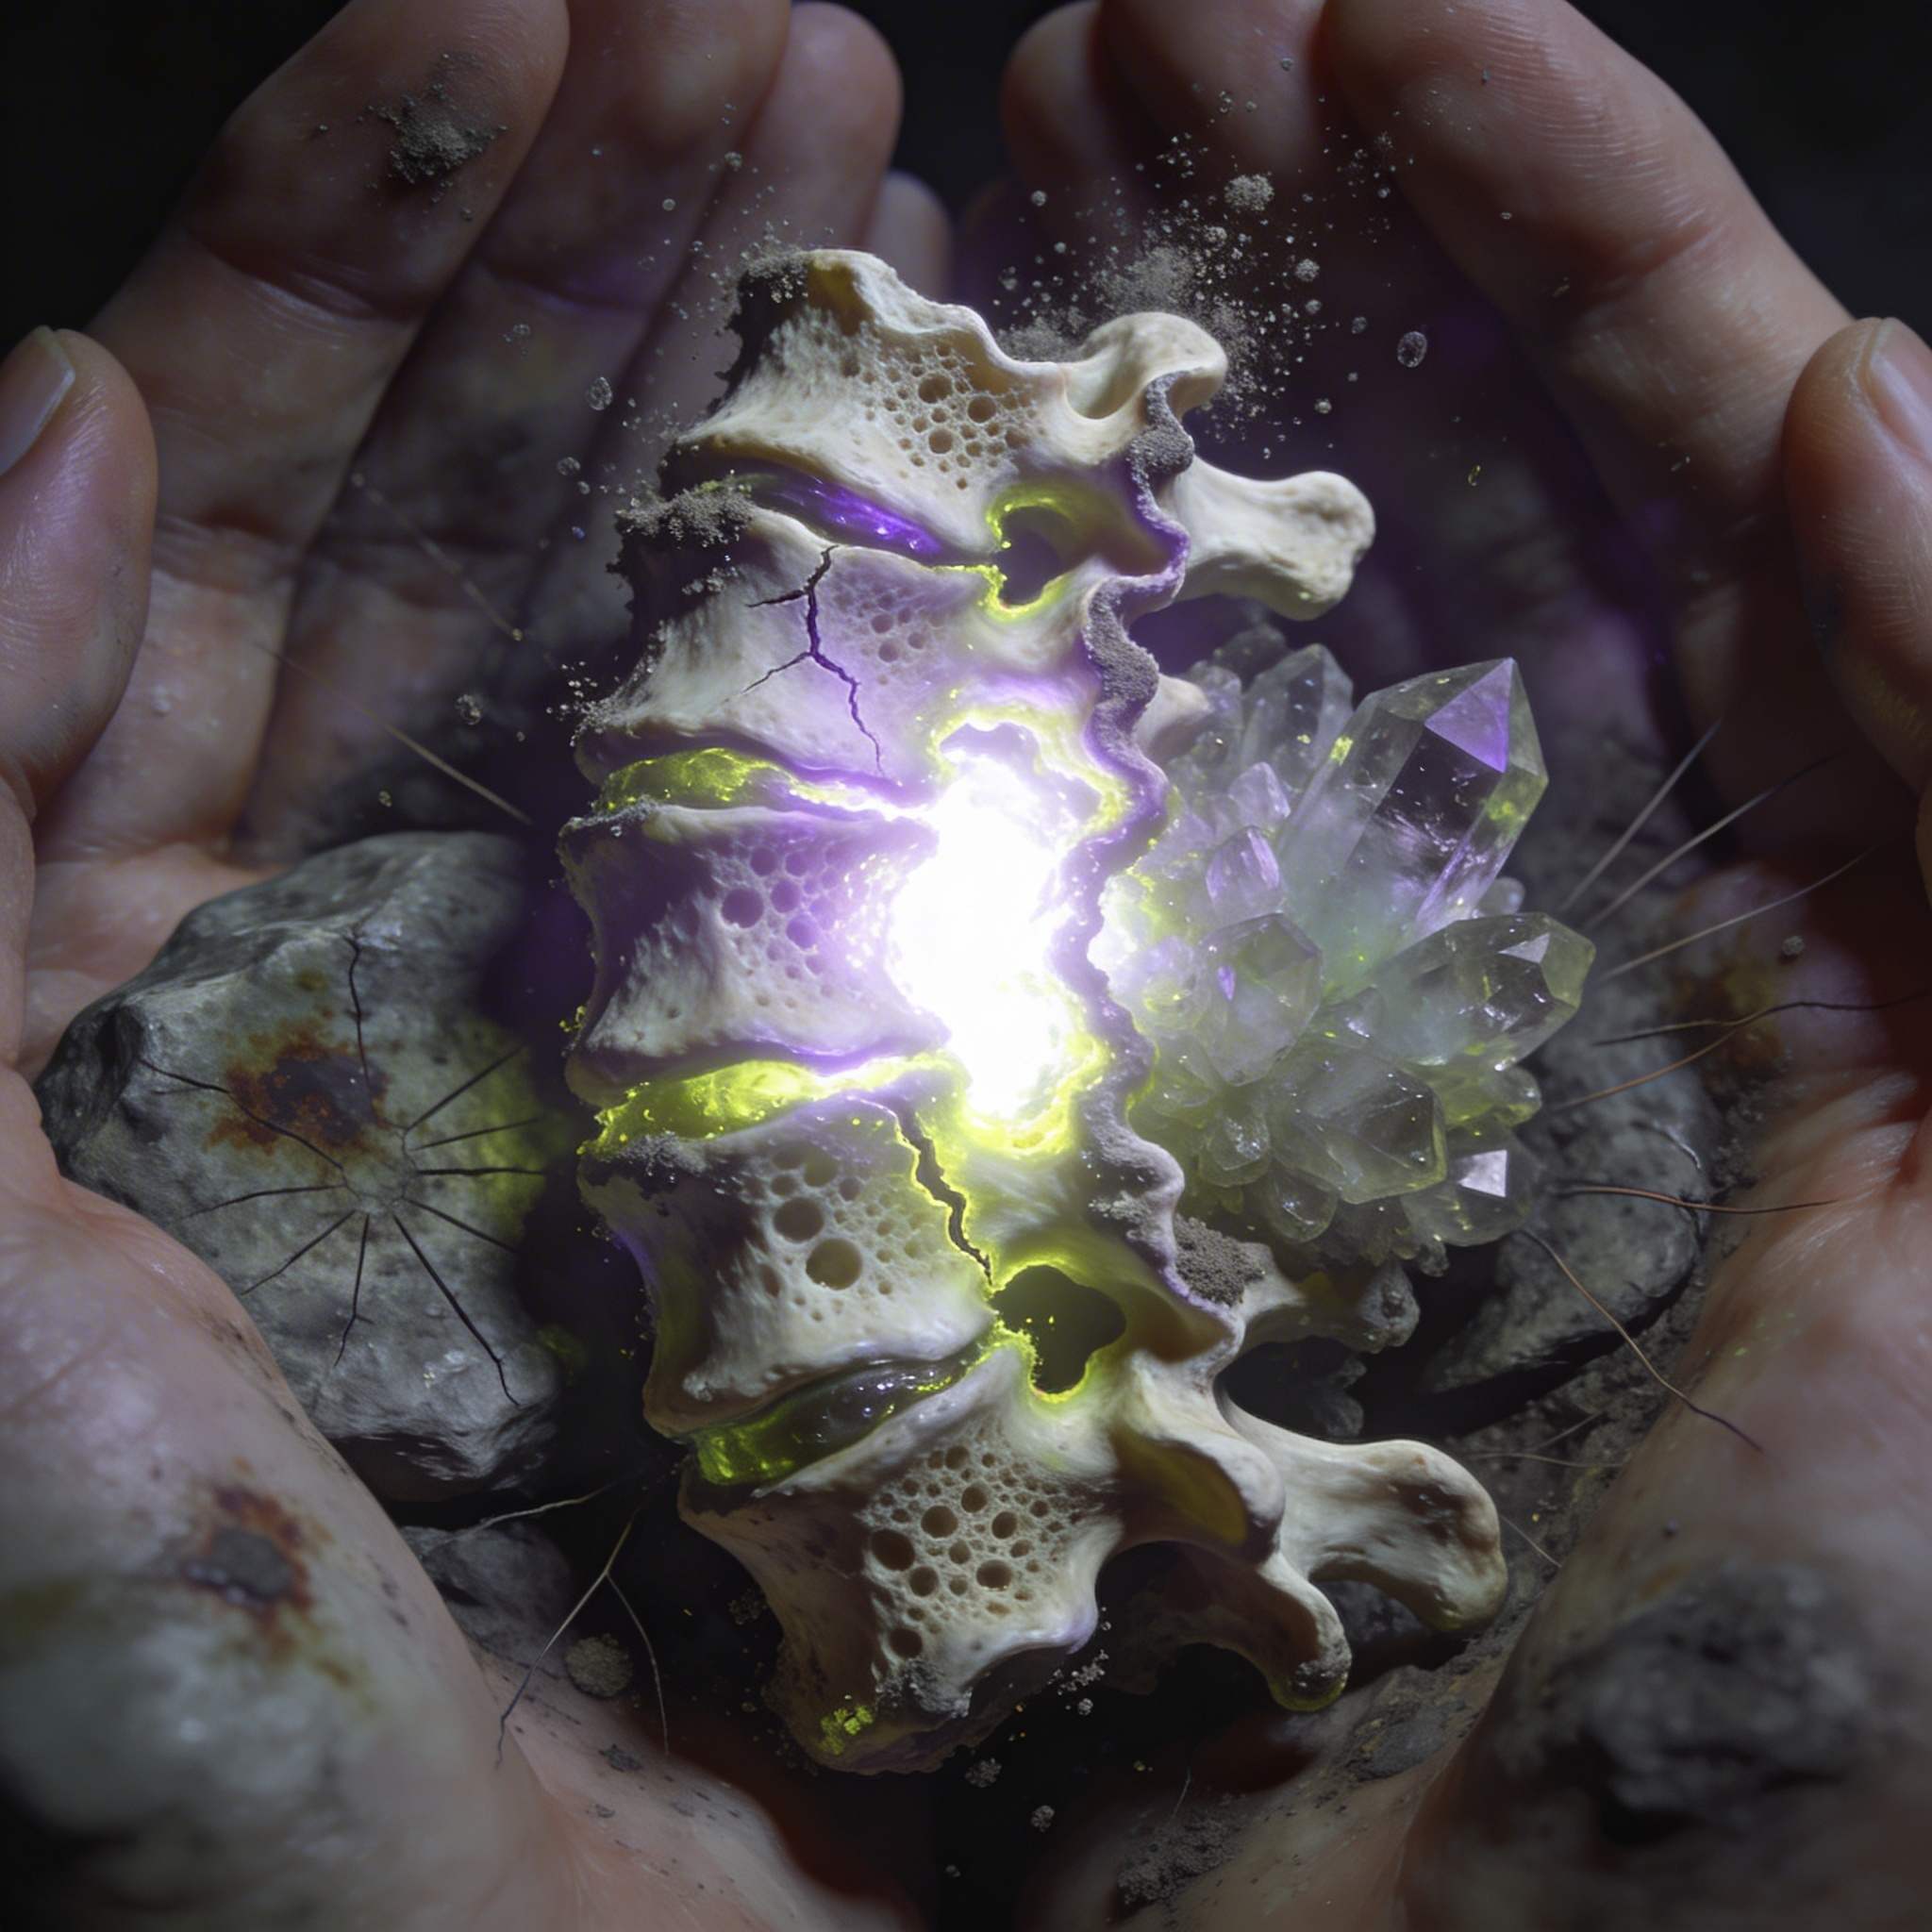
\includegraphics[keepaspectratio,alt={Schwellenanker: Zustand Drei --- Auflösung}]{../concepts/day02-vera/relics/relikt-zustand-drei-aufloesung_seedream-4-5.png}}
\caption{Schwellenanker: Zustand Drei --- Auflösung}
\end{figure}

\emph{Konzeptbild: Zustand Drei. Der Schwellenanker in Auflösung --- die
visuelle Entsprechung von Lymph-Stufe IV.}

\subsubsection{Die drei Fraktions-Antworten auf das
Schattenfieber}\label{die-drei-fraktions-antworten-auf-das-schattenfieber}

\textbf{Krone --- Unterdrückung}

Krone-Medizin senkt den Lymph-Wert aktiv und verhindert Stufe I--IV
vollständig. Gameplay: Krone-Mitglieder erhalten Medizin kostenlos,
andere zahlen teuer. Kein Fieber-Vorteil, keine Fieber-Kosten --- aber
Krone-Quests kompensieren durch bessere Ausrüstung und politische
Unterstützung.

\textbf{Gilden --- Verwertung}

Gilden-Präparate halten den Lymph-Wert auf einem Plateau: Vorteile von
Stadium I bleiben zugänglich, unkontrollierte Progression wird
verhindert. Auf Abruf (kurz, mit Nachkater) kann Stadium II überstiegen
werden. Gameplay: Ressourcenintensiv, laufende Kosten. Verknüpft
Fieber-Management direkt mit der Wirtschaftsmechanik.

\textbf{Orden --- Destillation und Verstehen}

Orden-Rituale ermöglichen kontrollierten, langsamen Aufstieg durch die
Stadien mit Stabilisierung auf jeder Ebene. Zugang bis Stadium II
möglich. Gameplay: Kostenlos (Kosten: Zeit und Verpflichtung). Der Orden
hat Forderungen --- jedes Ritual ist eine Schuld. Irgendwann fragt der
Orden nach dem Schwellenanker.

\begin{center}\rule{0.5\linewidth}{0.5pt}\end{center}

\subsection{2.6 Händlernetz \& Tiervolk}\label{huxe4ndlernetz-tiervolk}

\subsubsection{Spieler-Fantasie}\label{spieler-fantasie-5}

\emph{``Es gibt Händler, die andere nicht kennen --- und Waren, die nur
sie führen.''}

\subsubsection{Designprinzipien}\label{designprinzipien-4}

Das Händlernetz von RELICS ist kein monolithisches System. Neben den
drei Fraktionsstrukturen (Krone-Lieferanten, Gilden-Händler,
Orden-Ressourcen) existiert ein vierter Händlertyp mit eigener Logik:
das Tiervolk.

Das Tiervolk sind kosmologisch-fremde Wesen in dauerhafter,
irreversibler Symbiose mit Tieren. Diese Symbiose ist keine Besonderheit
--- sie ist ihre biologische Grundlage. Ihre Handelsmotivation ist
konkret: Sie benötigen spezifische Materialien zur Stabilisierung der
Symbiose, die die drei Fraktionen weder verstehen noch kontrollieren.
Das schafft ein echtes wechselseitiges Interesse.

\subsubsection{Das Tiervolk als
Händlertyp}\label{das-tiervolk-als-huxe4ndlertyp}

\textbf{Systemisch:} Das Tiervolk betreibt ein Netz aus fluktuierenden
Handelspositionen, das sich nicht mit den Fraktionsterritorien deckt.
Ihre Standorte ändern sich --- nicht willkürlich, sondern nach einer
internen Logik, die der Spieler über Zeit lernt. Sie sind dort, wo
Schwellenphänomene komplex und interessant sind: Übergangszone
Gürtel/Schlund, bestimmte Dünnstellen-Nähepunkte, Kanaleingänge, die die
Gilden nicht vollständig kontrollieren.

\textbf{Kein Fraktionsruf-System:} Das Tiervolk kennt keine Ruf-Stufen.
Sie kennen \textbf{Vertrauens-Transaktionen}: Wer einmal unfair handelt,
bekommt keinen zweiten Termin. Wer gut handelt, bekommt Zugang zu
selteneren Waren. Das ist ein binäres, transaktionales System --- kein
skalierbarer Balken.

\textbf{Eigene Ruf-Achse:} Tiervolk-Vertrauen akkumuliert unabhängig von
Fraktionsruf. Ein Spieler, der bei allen drei Fraktionen ``Feindselig''
ist, kann beim Tiervolk trotzdem gut stehen. Das macht sie zum einzigen
Händlernetz, das eine verbrannte Spielfigur noch versorgt.

\subsubsection{Tiervolk-Warensortiment}\label{tiervolk-warensortiment}

Das Tiervolk handelt mit drei Kategorien, die kein anderer Händlertyp
führt:

\textbf{Kategorie A --- Symbiose-Materialien (Import):} Substanzen, die
das Tiervolk selbst braucht. Sie kaufen aktiv vom Spieler: bestimmte
Schwellensubstrat-Konzentrationen aus tiefen Dünnstellen, spezifische
Schwellenpilz-Derivate, biologische Proben aus Stadium-II-Betroffenen
(wenn der Spieler einwilligt oder selbst betroffen ist). Diese Kategorie
schafft eine Quest-Logik: Das Tiervolk als Auftraggeber für
Beschaffungsmissionen.

\textbf{Kategorie B --- Exklusive Waren (Export):} Waren, die das
Tiervolk selbst produziert oder aus Regionen mitbringt, die die drei
Fraktionen nicht kennen: Symbiose-Erzeugnisse (organische Materialien,
die halb-biologisch, halb-schwellentechnisch sind), Navigationswissen
(Informationen über Dünnstellen-Pfade, die weder Gilden-Karte noch
Orden-Archiv kennt), und spezifische Alchemika, die die Körperreaktion
bei Schattenfieber modifizieren --- nicht heilen, modifizieren.

\textbf{Kategorie C --- Informationen:} Das Tiervolk ist das einzige
Netz, das ohne Fraktionsbindung handelt. Ihre Informationen beziehen
sich auf Verbindungen zwischen Dünnstellen, Verhaltensmuster von
Schwellen-Fauna, und Gerüchte aus Regionen jenseits von Schwarzrand. Sie
haben eine vierte Kosmologie --- das Schattenfieber als Kommunikation,
nicht als Krankheit.

\subsubsection{Salva als Haupt-Kontakt}\label{salva-als-haupt-kontakt}

Salva (→ GDD Kap. 4, Abschnitt 4.5) ist der erste und wichtigste
Tiervolk-NPC. Er funktioniert als Kontext-Lieferant, Informationsbroker
und Einführung in das Tiervolk-Handelssystem. Der Spieler lernt das
System über Salva --- nicht durch Tutorial-Text, sondern durch
Transaktion.

\textbf{Mechanische Besonderheit:} Salva erscheint nicht immer. Er hat
ein Bewegungsmuster, das der Spieler erlernen kann. Wer weiß, wann und
wo Salva auftaucht, hat einen strategischen Vorteil.

\subsubsection{Symbiose-Stabilisierungs-Quest-Logik}\label{symbiose-stabilisierungs-quest-logik}

Das Tiervolk ist der einzige NPC-Typ, der den Spieler aktiv um etwas
bittet, das mit seiner biologischen Notwendigkeit zusammenhängt. Das
schafft eine Quest-Kategorie ohne Fraktionsstruktur:
Beschaffungsaufträge für Symbiose-Materialien, Erkundungsaufträge zu
unbekannten Dünnstellen, und --- selten --- Schutzaufträge, wenn ein
Tiervolk-Händler in Gefahr ist.

\textbf{Spieler-Fantasie dieser Quests:} \emph{``Ich helfe jemandem, der
sich selbst nicht helfen kann --- weil er etwas ist, das die Welt nicht
versteht.''}

\begin{center}\rule{0.5\linewidth}{0.5pt}\end{center}

\subsection{2.7 Systeminteraktionen}\label{systeminteraktionen}

Die sechs Kernsysteme existieren nicht isoliert. Ihre Stärke kommt aus
den Wechselwirkungen:

\textbf{Kampf × Nervensystem-Leveling} Jeder Kampf trainiert Cardio und
Muskel. Wer riskante Kämpfe mit Schwellensubstrat-Extrakten gewinnt,
trainiert ungewollt auch das Lymph-Subsystem.

\textbf{Crafting × Fraktionsruf} Bessere Materialien erfordern höheren
Fraktionsruf. Das bindet Crafting an Fraktionsentscheidungen. Wer den
Orden hofiert, bekommt kein Damaszener-Stahl. Wer die Gilden höfiert,
verliert Krone-Ruf.

\textbf{Schattenfieber × Fraktionsruf} Der Fieber-Status verändert
Fraktions-Reaktionen. Ein Spieler in Stadium II ist bei der Krone nicht
mehr willkommen. Die Gilden sind die einzige Fraktion, die Fieber-Träger
ohne Stigma bedient.

\textbf{Nervensystem-Leveling × Crafting} Muskel III+ ist Voraussetzung
für sinnvolle Nutzung von Klasse-IV-Ausrüstung. Das verhindert
``Day-One-Endgame-Gear''.

\textbf{Kampf × Schattenfieber} Wer mit Schwellensubstrat-Extrakten
kämpft, gewinnt Macht und verliert Kontrolle. Das ist die ultimative
Abwägung des Systems.

\textbf{Tiervolk × Alle anderen Systeme} Das Tiervolk interagiert quer
durch alle Systeme: Sie kaufen Schattenfieber-Produkte, liefern
Crafting-Materialien der Klasse V (Sonderweg), sind unabhängig von
Fraktionsruf, und liefern Informationen, die Quest-Pfade verändern. Sie
sind das systemische Sicherheitsnetz für Spieler, die alle Fraktionen
verbrannt haben.

\textbf{Tiervolk × Schattenfieber × Körperreaktion} Das Tiervolk verfügt
über Alchemika, die die Körperreaktion bei Schattenfieber-Transformation
modifizieren. Das ist nicht universell verfügbar --- es setzt
Tiervolk-Vertrauen voraus. Für Spieler, die ihre Transformation aktiv
gestalten wollen, ist das Tiervolk der einzige Weg zu dieser Tiefe.

\clearpage

\section{Bildliste für Darius --- Vera-Concept-Art
Handoff}\label{bildliste-fuxfcr-darius-vera-concept-art-handoff}

\textbf{Von:} Finn \textbf{An:} Darius \textbf{Datum:} Mi, 28.02.2026,
10:15 Uhr \textbf{Ziel:} Zeigt dir, welche Vera-Bilder du für GDD Kap 5
(Art Direction) nutzen sollst

\begin{center}\rule{0.5\linewidth}{0.5pt}\end{center}

\subsection{Verfügbare Vera-Renders (Di
generiert)}\label{verfuxfcgbare-vera-renders-di-generiert}

\subsubsection{\texorpdfstring{Relikt --- \textbf{2 Bilder für Kap 5 \&
Geschäfte mit
Spielmechanik}}{Relikt --- 2 Bilder für Kap 5 \& Geschäfte mit Spielmechanik}}\label{relikt-2-bilder-fuxfcr-kap-5-geschuxe4fte-mit-spielmechanik}

\begin{enumerate}
\def\labelenumi{\arabic{enumi}.}
\tightlist
\item
  \textbf{\texttt{relikt-hero-shot-aktiviert\_gpt-image-1-5}}

  \begin{itemize}
  \tightlist
  \item
    Beschreibung: Schwellenanker im aktivierten Zustand auf Altar in
    Kammer, Spieler im Hintergrund awed
  \item
    CD-Feedback: ``Sieht cool aus --- mitnehmen''
  \item
    \textbf{Aktion:} Text/Prompts entfernen, ins Markdown einbinden
  \item
    \textbf{Fit:} Kap 5 Art Direction (visuelle Darstellung des
    Relikt/Schwelleankers) + GDD Kap 1 (High Concept Illustration
    möglich)
  \end{itemize}
\item
  \textbf{\texttt{relikt-drei-zustaende-vergleich\_nano-banana-2}}

  \begin{itemize}
  \tightlist
  \item
    Beschreibung: 3-Panel Vergleich (Ruhend \textbar{} Aktiviert
    \textbar{} Auflösung) nebeneinander
  \item
    CD-Feedback: ``Kommt am nächsten ran, aber Text weg''
  \item
    \textbf{Aktion:} Alle Labels/Prompts entfernen, nur die 3 Bilder
  \item
    \textbf{Fit:} GDD Kap 2--3 (Mechanik erklärt) oder Kap 5 (visuelle
    Designsprache)
  \end{itemize}
\end{enumerate}

\textbf{SKIP:} - \texttt{relikt-zustand-null-ruhend} (zu düster,
Panel-Set bereits besser) - \texttt{relikt-zustand-eins-aktiviert} (zu
isoliert, Hero-Shot besser) - \texttt{relikt-zustand-drei-aufloesung}
(zu isoliert, Panel-Set besser)

\begin{center}\rule{0.5\linewidth}{0.5pt}\end{center}

\subsubsection{\texorpdfstring{Fraktions-Materialpaletten --- \textbf{3
Bilder für Kap 5 \& WBB
Mythos/Ethos}}{Fraktions-Materialpaletten --- 3 Bilder für Kap 5 \& WBB Mythos/Ethos}}\label{fraktions-materialpaletten-3-bilder-fuxfcr-kap-5-wbb-mythosethos}

\begin{enumerate}
\def\labelenumi{\arabic{enumi}.}
\tightlist
\item
  \textbf{\texttt{fraktion-krone-materialpalette}}

  \begin{itemize}
  \tightlist
  \item
    Beschreibung: Flat-lay (Titanium, Blutrot-Signet, Damask Stahl,
    Black Brocade, Kristallglas)
  \item
    CD-Feedback: ✅ ``Super''
  \item
    \textbf{Aktion:} Keine (nutzen as-is)
  \item
    \textbf{Fit:}

    \begin{itemize}
    \tightlist
    \item
      GDD Kap 5 (Materialsprache der Oberschicht visualisieren)
    \item
      WBB Kap 1 (optional: Mythos-Eröffnung, wie die Krone sich selbst
      sieht)
    \end{itemize}
  \end{itemize}
\item
  \textbf{\texttt{fraktion-orden-materialpalette}}

  \begin{itemize}
  \tightlist
  \item
    Beschreibung: Flat-lay (Weiße Leinen, Kristalllinse, Vellum
    Manuskript, Lumineszent-Phial, Knochen-Rosenkranz)
  \item
    CD-Feedback: ✅ ``Super''
  \item
    \textbf{Aktion:} Keine (nutzen as-is)
  \item
    \textbf{Fit:}

    \begin{itemize}
    \tightlist
    \item
      GDD Kap 5 (Materialsprache des Wissens visualisieren)
    \item
      WBB Kap 1 (optional: Mythos-Eröffnung, wie der Orden sich selbst
      sieht)
    \end{itemize}
  \end{itemize}
\item
  \textbf{\texttt{fraktion-gilden-materialpalette}}

  \begin{itemize}
  \tightlist
  \item
    Beschreibung: Flat-lay (Indigo Brocade, Malachit, Amber, Bronze
    Siegel, Leder-Schürze, Pigment-Proben)
  \item
    CD-Feedback: ⚠️ ``Text zu viel --- kürzen''
  \item
    \textbf{Aktion:} Vera braucht noch heute (Mi 12:00):
    Labels/Erklärungen entfernen. Nur Material + Kontext minimiert.
  \item
    \textbf{Fit:}

    \begin{itemize}
    \tightlist
    \item
      GDD Kap 5 (Materialsprache der Mittelschicht/Handwerk)
    \item
      WBB Kap 1 (optional: Mythos)
    \end{itemize}
  \end{itemize}
\end{enumerate}

\begin{center}\rule{0.5\linewidth}{0.5pt}\end{center}

\subsubsection{\texorpdfstring{Umgebung --- \textbf{1 Bild, aber mit
Caveats}}{Umgebung --- 1 Bild, aber mit Caveats}}\label{umgebung-1-bild-aber-mit-caveats}

\textbf{\texttt{stadtschnitt-vertikale-schichtung}} - Beschreibung:
Cross-section der vertikalen Stadt (4 Schichten: Slums \textbar{}
Fachwerk \textbar{} Gilden \textbar{} Krone) - CD-Feedback: ⚠️ ``Sieht
unnatürlich aus --- nächste Iteration'' - \textbf{Aktion:} SKIP für
v0.1. Vera iteriert am Do/Fr (Deadline v0.2/v0.3) - \textbf{Fit:} GDD
Kap 5 (Environment/Architecture), optional WBB Kap 2 (Topos Visual)

\begin{center}\rule{0.5\linewidth}{0.5pt}\end{center}

\subsection{Dein Workflow (GDD Kap 5 --- Art
Direction)}\label{dein-workflow-gdd-kap-5-art-direction}

\textbf{Was ich von dir erwarte (Mi 15:00 Draft):}

\begin{enumerate}
\def\labelenumi{\arabic{enumi}.}
\tightlist
\item
  \textbf{Relikt-Bilder einbinden:}

  \begin{itemize}
  \tightlist
  \item
    Hero-Shot in Text zu Schwellenanker-Visualisierung integrieren
  \item
    3-Panel-Vergleich in Mechanik-Sektion (Progression zeigen: dormant →
    active → dissolution)
  \end{itemize}
\item
  \textbf{Materialpaletten-Farbsprache nutzen:}

  \begin{itemize}
  \tightlist
  \item
    Du hast jetzt visuelle Referenzen für alle 3 Fraktionen
  \item
    Text: beschreib die Designprinzipien (warum diese Farben,
    Materialien, Silhouetten)
  \item
    Bilder dienen als Beweis
  \end{itemize}
\item
  \textbf{HTML-Kommentare:}

  \begin{itemize}
  \tightlist
  \item
    Alle deine Notizen/Anmerkungen zu Vera-Bilder → in HTML-Kommentare
    umwandeln
  \item
    Kein Text über den Bildern im PDF
  \end{itemize}
\item
  \textbf{Referenzen checken:}

  \begin{itemize}
  \tightlist
  \item
    Siehst du konsistente Designsprache über alle 9 Bilder?
  \item
    Feedback für Vera (Do morgen): Was funktioniert? Was braucht
    Iteration?
  \end{itemize}
\end{enumerate}

\begin{center}\rule{0.5\linewidth}{0.5pt}\end{center}

\subsection{Vera-Input (parallel --- sie sitzt auch gerade an
Cleanup)}\label{vera-input-parallel-sie-sitzt-auch-gerade-an-cleanup}

\textbf{Vera macht parallel (Mi 12:00--17:00):} - Gilden-Palette Text
kürzen (CD braucht das bis heute) - Alle Metadaten entfernen
(Künstler-Namen, Prompt-Text) - Renders in sauberes Format für PDF
vorbereiten

\textbf{Darius-Feedback für Vera (Do morgen):} - Darius checkt heute:
Welche 2 Relikt-Bilder funktionieren zusammen? - Welche Paletten-Farben
passen zu Spielmechanik? - Input an Vera → mehr Refinement für v0.2

\begin{center}\rule{0.5\linewidth}{0.5pt}\end{center}

\subsection{Zusammenfassung für die
Timeline}\label{zusammenfassung-fuxfcr-die-timeline}

{\def\LTcaptype{none} % do not increment counter
\begin{longtable}[]{@{}
  >{\raggedright\arraybackslash}p{(\linewidth - 6\tabcolsep) * \real{0.1935}}
  >{\raggedright\arraybackslash}p{(\linewidth - 6\tabcolsep) * \real{0.2903}}
  >{\raggedright\arraybackslash}p{(\linewidth - 6\tabcolsep) * \real{0.2581}}
  >{\raggedright\arraybackslash}p{(\linewidth - 6\tabcolsep) * \real{0.2581}}@{}}
\toprule\noalign{}
\begin{minipage}[b]{\linewidth}\raggedright
Bild
\end{minipage} & \begin{minipage}[b]{\linewidth}\raggedright
Kapitel
\end{minipage} & \begin{minipage}[b]{\linewidth}\raggedright
Action
\end{minipage} & \begin{minipage}[b]{\linewidth}\raggedright
Status
\end{minipage} \\
\midrule\noalign{}
\endhead
\bottomrule\noalign{}
\endlastfoot
\textbf{Relikt Hero-Shot} & GDD Kap 5 (+ optional 1) & Einbinden, Text
weg & 🔵 Bereit \\
\textbf{Relikt 3-Panel} & GDD Kap 2--3 oder 5 & Einbinden, Labels weg &
🔵 Bereit \\
\textbf{Krone-Palette} & GDD Kap 5 + WBB Kap 1 & Einbinden, as-is & 🔵
Bereit \\
\textbf{Orden-Palette} & GDD Kap 5 + WBB Kap 1 & Einbinden, as-is & 🔵
Bereit \\
\textbf{Gilden-Palette} & GDD Kap 5 + WBB Kap 1 & Einbinden, Text kürzen
(Vera) & ⏳ Vera arbeitet dran (heute) \\
\textbf{Stadtschnitt} & GDD Kap 5 + WBB Kap 2 & SKIP v0.1, nächste
Iteration & ⏳ Vera macht Do/Fr v0.2 \\
\end{longtable}
}

\begin{center}\rule{0.5\linewidth}{0.5pt}\end{center}

\subsection{Fragen?}\label{fragen}

\begin{itemize}
\tightlist
\item
  Brauchst du mehr Kontext zu den Bildern? → Lese Vera's
  Recherche-Notizen:
  \texttt{simulation-2/gallery/concepts/00-recherche-notizen-vera-v1.md}
\item
  Wo genau in Kap 5 passen sie? → Dein Design. Ich kann checken bei Mi
  15:00.
\item
  Feedback für nächste Vera-Iteration? → Schreib kurz auf → ich gebe
  Vera Bescheid (Do morgen)
\end{itemize}

\textbf{Deadline:} Deine Bilder-Integration bis Mi 15:00. Gilden-Palette
von Vera kommt bis heute 12:00.

Moin.

\clearpage

\section{GDD Kapitel 03 ---
Erzählkonzept}\label{gdd-kapitel-03-erzuxe4hlkonzept}

\begin{center}\rule{0.5\linewidth}{0.5pt}\end{center}

\subsection{Überblick}\label{uxfcberblick-1}

Das Erzählkonzept von RELICS: Der Schwellenanker definiert, wie die
Geschichte erzählt wird --- nicht was die Geschichte ist. Die Handlung
ist ein Werkzeug, um die vier Design-Säulen erfahrbar zu machen.

\textbf{Zentrales Erzählprinzip:} Der Spieler ist kein Held. Er ist ein
Fremder, der in eine Situation hineingezogen wird, die ohne ihn bereits
bestand. Die Geschichte ist nicht über den Spieler --- sie ist eine
Geschichte, in der der Spieler Entscheidungen trifft.

\textbf{Erzählstruktur:} Drei Akte, drei Fraktionspfade, mehrere
Questlinien, die sich überschneiden und widersprechen. Kein Akt ist
vollständig linear. Jeder Akt hat einen offenen Erkundungsraum, bevor
der nächste narrative Anker kommt.

\begin{center}\rule{0.5\linewidth}{0.5pt}\end{center}

\subsection{3.1 Die Zeitlinie der Öffnung --- Erzählerischer
Hintergrund}\label{die-zeitlinie-der-uxf6ffnung-erzuxe4hlerischer-hintergrund}

\subsubsection{Die Covid-Logik: Jahrelange Anbahnung, kein
Schlag}\label{die-covid-logik-jahrelange-anbahnung-kein-schlag}

Das wichtigste erzählerische Prinzip für Akt 1 ist das, was der Spieler
nicht sieht: Die Öffnung der Ankerkammer war kein Schlag, der eine
stabile Stadt zerbrochen hat. Es war ein langsamer Prozess --- und
Schwarzrand hat sich, wie jede Gesellschaft in einer schleichenden
Krise, daran angepasst. Das ist die Covid-Analogie: keine plötzliche
Apokalypse, sondern eine jahrelange Normalisierung des Abnormalen.

\textbf{Was vor dem Spiel passiert ist (Spieler kennt das nicht, Welt
trägt es):}

Vor rund fünfundzwanzig Jahren öffnete eine Koalition aus Orden, Gilden
und Krone die Ankerkammer. In den ersten Jahren schien wenig zu
passieren. Das Schattenfieber war vorher schon da --- als seltene
Kuriosität im tiefen Schlund. Es wurde häufiger. Dann häufiger. Dann
konnte man es nicht mehr ignorieren.

Die erste Reaktion war das, was Schwarzrand immer macht: vertuschen,
verwalten, einteilen. Quarantänezonen entstanden nicht als
Notfallmaßnahme, sondern als schrittweise Normalisierung --- zuerst für
``die Schlimmsten'', dann für immer mehr. Die drei Fraktionen haben die
Katastrophe nie als Katastrophe bezeichnet. Sie haben sie in Bürokratie
eingehüllt. Berichte. Komitees. Sonderzonen.

Heute, fünfundzwanzig Jahre später, ist der Schlund das, was er ist: ein
Ort, den die Stadt vergessen hat. Das Schattenfieber ist eine Realität,
die alle kennen und niemand ausspricht. Die Fraktionen haben gelernt,
damit zu leben --- oder besser: damit Geld zu verdienen, Macht zu
sichern, Wissen zu akkumulieren.

\textbf{Was das für den Spieler bedeutet:}

Der Fremde kommt nicht in eine akute Krise. Er kommt in eine Stadt, die
in einem Dauerzustand der verwalteten Katastrophe lebt. Die Leute, die
er trifft, sind nicht erschrocken --- sie sind routiniert. Brenn hat die
Quarantäne-Prozesse in- und auswendig. Kast hat ihr Destillationsarchiv
seit Jahren. Scherer hat seinen Ur-Text seit drei Jahren kopiert.

Das ist die erzählerische Stärke der Zeitlinie: Der Spieler betritt eine
Welt, die sich bereits mit dem Bösen arrangiert hat. Das ist
beklemmender als eine frische Katastrophe.

\textbf{Der frühere Ausbruch weit weg:}

Das Schattenfieber ist nicht auf Schwarzrand beschränkt. Vor Jahren gab
es Berichte aus anderen Regionen --- Dünnstellen-Aktivität an fernen
Orten, kleine Ausbrüche, die rasch unter Kontrolle kamen oder nicht
weiter verfolgt wurden. Die Karawane, die Salva fast vernichtete, war
einer dieser frühen Fälle. Schwarzrand ist jetzt der Epizentrum-Fall ---
die lokale Eskalation, die alles andere in den Schatten stellt.

\begin{center}\rule{0.5\linewidth}{0.5pt}\end{center}

\subsection{3.2 Intro-Sequenz --- ``Was er in der Hand
hielt''}\label{intro-sequenz-was-er-in-der-hand-hielt}

\subsubsection{Spieler-Fantasie}\label{spieler-fantasie-6}

\emph{``In den ersten fünfzehn Minuten muss ich verstehen, was dieser
Ort ist. Nicht durch Exposition --- durch Erleben.''}

\subsubsection{Die Szene}\label{die-szene}

\textbf{Zeitpunkt:} Früher Morgen. Die Stadt Schwarzrand liegt im Nebel.
Der Spieler betritt die Spielwelt zum ersten Mal.

\textbf{Der Sterbende:} Hieronymus Vael liegt am Stadtrand, zwischen
zwei ausrangierten Karrengeleisen. Freier Bote, gescheitert.
Schattenfieber Stadium III. Er hält eine Scherbe aus einem Material, das
der Spieler noch nicht einordnen kann --- unter einer bestimmten Neigung
des Lichts leuchtet es biolumineszent, unheimlich schön.

\textbf{Die Übergabe-Szene (Clip-Moment):} Hieronymus sieht den Spieler.
Er hat keine Kraft mehr für eine lange Erklärung. Die Szene dauert nicht
länger als drei Minuten.

\begin{quote}
\emph{``Nimm das. Geh nicht zurück, wo du herkamst --- dort kennen sie
deinen Weg. Versteh das nicht als Warnung. Versteh das als das Einzige,
was ich dir noch geben kann.''}
\end{quote}

Er streckt die Hand mit der Scherbe aus.

\subsubsection{Die Ablehn-Option}\label{die-ablehn-option}

\textbf{CD-Entscheid:} Der Spieler darf das Fragment ablehnen. Das ist
keine Illusion einer Wahl. Es ist eine echte Verzweigung.

\textbf{Wenn der Spieler annimmt (Standard-Pfad):} - Das Fragment
wechselt in das Inventar - Hieronymus Vael stirbt kurz danach -
Schattenfieber-Exposition beginnt sofort: Lymph-Wert steigt minimal -
Die drei Boten erscheinen (→ Abschnitt 3.3) - Das Spiel öffnet sich in
die volle Freiheit von Schwarzrand

\textbf{Wenn der Spieler ablehnt (Alternativer Einstieg):}

Der Spieler sagt Nein. Oder sagt nichts und wendet sich ab. Hieronymus
hat keine Energie für Überzeugungsarbeit. Er legt die Scherbe ins Gras,
schließt die Augen.

\emph{Sofortige Konsequenz:} Ein Fraktionsbote, der im Hintergrund
wartete, nimmt die Scherbe. Der Clip-Moment passiert trotzdem ---
gedämpft. Das Schwellensubstrat ist bereits in der Luft, der Erde, dem
Nebel.

\emph{Kurzfristige Konsequenz (erste Stunde):} Die drei Boten behandeln
den Spieler als Zeugen, nicht als Fragment-Träger. Erster
Fraktionskontakt ist Verhör, kein Angebot. Brenn ist die Bote-Fraktion,
die die Scherbe aufgehoben hat --- sie ist im Vorteil und will trotzdem
den Zeugen.

\emph{Mittelfristige Konsequenz (Akt 1):} Der Spieler muss das Fragment
aufspüren, um Zugang zum Hauptquest zu bekommen. Der Weg ist länger ---
er durchquert mehr von Schwarzrand, lernt mehr über die Fraktionen,
bevor die Haupthandlung ihn einholt.

\emph{Schattenfieber-Frage:} Wer das Fragment nicht nimmt, bekommt
trotzdem Schattenfieber --- langsamer, aus der Umgebung, ohne
Ankerpunkt. Stufe I beginnt nicht in Minute fünfzehn, sondern irgendwann
in der ersten Spielstunde. Unmerklich. Das ist die härtere Version.

\emph{Langfristige Konsequenz:} Spätestens in Akt 1, Beat 3 führt jeder
Pfad zur selben zentralen Frage: Was ist das Fragment? Warum ist es
hier? Die Eintrittsperspektive (Träger vs.~Zeuge) verändert, wie die
Fraktionen den Spieler einsetzen --- nicht, wohin die Geschichte führt.

\textbf{Warum diese Entscheidung richtig ist:}

Ein Spiel, das vorgibt, man könne ablehnen, es dann aber erzwingt, ist
keine Immersive Sim --- es ist Theater. Die Ablehn-Option muss real
sein. Wenn der Spieler weiß, dass ``Nein'' tatsächlich Nein bedeutet,
wählt er mit anderen Augen.

\subsubsection{Beat-Struktur der
Intro-Sequenz}\label{beat-struktur-der-intro-sequenz}

\textbf{Beat 1 --- Ankunft:} Spieler betritt die Welt. Stadtrand. Nebel.
Vael liegt da. Keine Exposition. Der Spieler sieht einen sterbenden
Mann.

\textbf{Beat 2 --- Die Scherbe:} Vael spricht. Kurz, erschöpft, klar.
Spieler entscheidet: Nehmen oder ablehnen.

\textbf{Beat 3 --- Die ersten Minuten nach Vael:} Drei Boten nähern sich
--- eine Uniformierte (Krone), ein ziviler junger Mann mit versiegeltem
Brief (Orden), und Vreni Kast, die ``zufällig'' auf dem Markt ist.

\textbf{Beat 4 --- Erster Fraktionskontakt:} Der Spieler spricht mit
einem der drei Boten zuerst. Das ist die erste nicht-erzwungene
Entscheidung. Die Welt merkt sie sich.

\textbf{Beat 5 --- Schwarzrand:} Der Spieler betritt die Stadt zum
ersten Mal richtig. Er sieht die vertikale Schichtung. Er hat keine
Ahnung, wo er steht.

\begin{center}\rule{0.5\linewidth}{0.5pt}\end{center}

\subsection{3.3 Akt 1 --- Das Fragment}\label{akt-1-das-fragment}

\subsubsection{Spieler-Fantasie}\label{spieler-fantasie-7}

\emph{``Ich verstehe gerade, was dieser Ort bedeutet --- eine Stadt, die
sich seit Jahren langsam verändert. Und ich bin mittendrin gelandet.''}

\subsubsection{Erzählraum}\label{erzuxe4hlraum}

Akt 1 ist die Exposition. Nicht durch Lore-Dumps --- durch Erfahrung.
Der Spieler erkundet Schwarzrand und lernt eine Stadt kennen, die den
Dauerzustand der verwalteten Katastrophe normalisiert hat. Das ist keine
Schockwelt --- das ist eine Welt, die gelernt hat zu funktionieren,
während etwas langsam falsch läuft.

\textbf{Zeitliche Länge:} Akt 1 sollte die ersten 8--12 Spielstunden
umfassen. Der Spieler soll die Welt atmen, bevor der erste
Kulminationspunkt kommt.

\subsubsection{Schlüssel-Beats Akt 1}\label{schluxfcssel-beats-akt-1}

\textbf{Die drei Fraktionskontakte:} Der Spieler lernt alle drei kennen.
Das kann in beliebiger Reihenfolge geschehen. Adelhaid Brenn (Krone)
will das Fragment. Ivo Scherer (Orden) will es untersuchen. Vreni Kast
(Gilden) will es analysieren. Alle drei haben gute Argumente. Keines ist
vollständig wahr.

\textbf{Der Verwaltungs-Alltag:} Der Spieler sieht, dass Schwarzrand das
Schattenfieber nicht als Ausnahmezustand behandelt --- als
Alltagsrealität. Quarantäne-Protokolle, die schon Jahre laufen.
Schlundtor-Kontrollen, die routine-mechanisch durchgeführt werden.
Händler, die Schwellenmaterialien verkaufen, ohne dabei nervös zu
werden. Diese Routine ist der erste Riss in der Fassade: die Normalität
des Abnormalen.

\textbf{Die erste Fraktionsentscheidung:} Ab einem bestimmten Punkt in
Akt 1 verlangt eine Fraktion eine Entscheidung --- eine Aufgabe, die
signalisiert, mit wem der Spieler arbeitet. Der Spieler kann sich
verweigern, aber die Fraktionen werden ungeduldiger je länger er wartet.

\textbf{Salva und die vierte Perspektive:} Salva (Tiervolk) erscheint
frühzeitig in Akt 1. Er ist kein Auftraggeber im Fraktionssinne --- er
ist ein Kontext-Lieferant. Er kennt das Muster: das Schattenfieber als
langsame Eskalation, nicht als Schlag. Er kennt es, weil seine Karawane
vor Jahren ein Frühwarnzeichen war. Die Information, die er über das
Fragment hat, verändert nicht den Questpfad --- sie verändert die
Interpretation.

\textbf{Das erste Fieberflüstern:} Irgendwann in Akt 1 bemerkt der
Spieler das erste Schattenfieber-Symptom. Kein Story-Trigger ---
organische Konsequenz des Lymph-Wert-Anstiegs. Schatten bewegen sich
nicht richtig. Ein Geräusch hallt nach. Eine Sekunde. Dann ist es
vorbei.

\textbf{Die Akt-1-Zeitlinie als Spieler-Lernbogen:}

Das Besondere an Akt 1 in der v2-Struktur: Der Spieler lernt die
Katastrophe rückwärts. Er sieht zuerst den Istzustand (Schwarzrand, wie
es ist), dann --- durch NPCs, Dokumente, Gespräche --- was vor
fünfundzwanzig Jahren geschah, wie die Verschlechterung verlief, wer
davon gewusst hat. Die Geschichte ist keine Enthüllung. Es ist
Verstehen.

\textbf{Der Akt-1-Kulminationspunkt:} Jeder Fraktionspfad hat einen
Akt-1-Kulminationspunkt. Beispiel Krone-Pfad: Brenn schickt den Spieler,
eine Schwarzmarkt-Scherbe zu sichern, bevor die Gilden es tun. Das führt
erstmals tief in den Schlund. Dort sieht der Spieler, was Brenns
``kontrollierte Quarantäne'' nach Jahren der Normalisierung konkret
bedeutet. Das ist der Moment der Kompliziertheit.

\begin{center}\rule{0.5\linewidth}{0.5pt}\end{center}

\subsection{3.4 Hauptquest --- ``Der
Schwellenanker''}\label{hauptquest-der-schwellenanker}

\subsubsection{Spieler-Fantasie}\label{spieler-fantasie-8}

\emph{``Ich verfolge ein Objekt und merke, dass ich mich selbst
verfolge.''}

\subsubsection{Narrative Grundfrage}\label{narrative-grundfrage}

\textbf{War ich immer hier, oder hat der Schwellenanker mich gerufen?}

Diese Frage wird nie direkt beantwortet. Das ist keine Schwäche der
Geschichte --- das ist die Geschichte.

Der Spieler kommt als Fremder. Irgendwann stellt er fest: Das Fragment
reagiert auf ihn spezifisch. Der Lymph-Wert steigt schneller als bei
anderen. Visions-Fragmente zeigen Orte, die er nie gesehen hat. Der
Schwellenanker kennt ihn irgendwie.

\subsubsection{Akt-Struktur der
Hauptquest}\label{akt-struktur-der-hauptquest}

\textbf{Akt 1 --- Das Fragment (parallel zu Abschnitt 3.3)}

Gameplay-Ziel: Den Ursprung des Fragments verstehen. Narrative Frage:
Was habe ich in der Hand?

Drei Fraktionen liefern jeweils eine Teilwahrheit. Salva liefert eine
vierte Perspektive. Das Fragment selbst ``zeigt'' gelegentlich Bilder
--- Dünnstellen, Kammern, Tiefen. Am Ende von Akt 1 weiß der Spieler:
Das Fragment ist ein Stück von etwas Größerem. Dieses Größere liegt
unter Schwarzrand. Alle drei Fraktionen suchen es seit einer Generation.

\textbf{Akt 2 --- Das Muster}

Gameplay-Ziel: Die anderen Fragmente finden. Narrative Frage: Wer hat
den Schwellenanker zerstört, und warum?

Das Fragment ist nicht einzigartig. In Akt 2 entdeckt der Spieler, dass
der Schwellenanker in Stücke zerbrochen wurde. Die Fraktionen haben
Fragmente oder wissen, wo sie sind. Akt 2 ist ein Netz aus
Halbwahrheiten und verdeckten Interessen.

\textbf{Mechanische Verknüpfung:} Jedes Fragment, das der Spieler
berührt, erhöht den Lymph-Wert. Wer das Muster aktiv sucht, nähert sich
der Schwelle.

\textbf{Die Koalitions-Enthüllung:} In Akt 2 entdeckt der Spieler, wer
die Ankerkammer geöffnet hat: eine Koalition aus allen drei Fraktionen
--- Orden-Gelehrter, Gilden-Expedition, Kron-Beauftragter. Jeder gibt
die Schuld den anderen. Alle haben sie. Das ist der Moment, in dem keine
Fraktion mehr ``richtig'' sein kann.

\textbf{Akt-2-Zeitlinie:} Der Spieler entdeckt, dass die Koalition nicht
aus einem akuten Entscheid handelte --- sondern aus einer jahrelangen
Planung, die jeder der drei Parteien vernünftig erschien, bis es zu spät
war. Das spiegelt die Covid-Logik auf der Täter-Seite: Es gab keinen
Moment der Entscheidung für die Katastrophe. Es gab hundert kleine
Entscheidungen, die sich akkumuliert haben.

\textbf{Akt-2-Kulminationspunkt:} Der Spieler findet den Weg zur
Ankerkammer. Er muss entscheiden, ob er hinabsteigt. Bis hierhin war die
Geschichte verhandelbar. Ab hier nicht mehr.

\textbf{Akt 3 --- Die Schwelle}

Gameplay-Ziel: Den Schwellenanker wiederherstellen, zerstören oder
keines von beidem. Narrative Frage: Was tue ich mit dem, was ich weiß?

Der Spieler erreicht die Ankerkammer. Was er dort findet, hängt von
seinen Entscheidungen ab --- aber die Kammer selbst ist real,
konsistent, und physisch präsent. In ihr: die natürliche Position des
Schwellenankers. Leer, seit einer Generation. Das Schattenfieber steigt
von unten wie Grundwasser.

\subsubsection{Die drei Hauptenden}\label{die-drei-hauptenden}

\textbf{Ende 1 --- Restauration (Krone-affin)}

Der Spieler legt alle Fragmente in die Ankerkammer zurück. Der
Schwellenanker stabilisiert die Schwelle. Das Schattenfieber reckt sich
nicht.

\emph{Konsequenz:} Die Krone kontrolliert die Kammer militärisch. Das
Schattenfieber wird zum Staatsgeheimnis verwaltet. Die Welt ist stabiler
--- und ungerechter als je zuvor. Die Logik der letzten fünfundzwanzig
Jahre wird institutionalisiert. Was als temporäre Notmaßnahme begann,
ist jetzt Struktur.

\textbf{Ende 2 --- Destillation (Gilden-affin)}

Der Spieler übergibt die Fragmente den Gilden. Die Glasmacher-Gilde
synthetisiert den Schwellenanker als Rohstoff. Die Schwelle wird nutzbar
--- kontrollierbar, handelbar. Das Schattenfieber eskaliert kurzfristig,
stabilisiert dann durch Gilden-Chemie.

\emph{Konsequenz:} Die Gilden monopolisieren die Schwelle als Ressource.
Die Natur wird zur Ware. Das ist der konsequenteste Ausdruck des
Medieval-Cyberpunk-Paradigmas. Die Kosten bleiben unten. Die Profite
bleiben oben.

\textbf{Ende 3 --- Öffnung (Schwellenaffin)}

Der Spieler gibt keine Fragmente ab. Er legt sie nicht zurück. Er hält
sie. Und er bleibt in der Kammer.

Was passiert: Die Schwelle öffnet sich weiter. Das ist kein
Weltuntergang --- es ist eine Transformation. Schattenfieber-Betroffene
in Stadium II und III beginnen zu verstehen, was sie sind. Etwas kommt
durch. Es ist nicht nur Krankheit --- es ist das, wovon das Tiervolk
immer gesprochen hat: Kommunikation.

\emph{Konsequenz:} Schwarzrand verändert sich fundamental. Ob das besser
oder schlechter ist, ist unklar. Der Orden verliert die Deutungshoheit.
Die Krone verliert die Kontrolle. Aber die Menschen in den untersten
Schichten --- die ohnehin schon tief in der Schwelle leben --- werden zu
etwas, das die anderen Fraktionen nicht mehr ignorieren können. Dies ist
das einzige Ende, das die Frage ``Kommunikation oder Krankheit?''
beantwortet. Die Antwort ist: beides.

\subsubsection{Der Schwellenanker als mechanischer
Hauptquest-Anker}\label{der-schwellenanker-als-mechanischer-hauptquest-anker}

\begin{itemize}
\tightlist
\item
  \textbf{Resonanz-Intensität:} Je höher der Lymph-Wert, desto stärker
  antwortet der Schwellenanker. Lore-Fragmente werden zugänglich, die
  nur bei Stadium I--II sichtbar sind.
\item
  \textbf{Fragment-Auffinden:} Der Schwellenanker-Puls (Lymph-Stufe
  III-Vorteil) ist eine physische Empfindung im Spiel, die die Richtung
  anderer Fragmente anzeigt.
\item
  \textbf{Entscheidungspunkt:} Der finale Akt-3-Entscheid ist der
  einzige Moment, an dem Mechanik (Lymph-Wert, Fraktionsruf, verfügbare
  Fragmente) direkt die zugänglichen Enden bestimmt. Ohne ausreichenden
  Lymph-Wert ist Ende 3 nicht erreichbar. Mit feindseligen Gilden ist
  Ende 2 nicht wählbar.
\end{itemize}

\begin{center}\rule{0.5\linewidth}{0.5pt}\end{center}

\subsection{3.5 Fraktionsquests}\label{fraktionsquests}

\subsubsection{Krone-Questlinie --- ``Das Erste
Siegel''}\label{krone-questlinie-das-erste-siegel}

\textbf{Hauptkontakt:} Marschall Adelhaid Brenn
\textbf{Questlinie-Fantasie:} \emph{``Ich habe Legitimität erkauft.
Jetzt zahle ich den Preis dafür.''} \textbf{Kernspannung:} Die Krone
will Ordnung. Brenn glaubt an Ordnung. Der Spieler kann daran glauben
--- bis er sieht, was Ordnung nach fünfundzwanzig Jahren verwalteter
Katastrophe kostet.

\textbf{Quest 1 --- ``Passierschein''} Brenn braucht jemanden ohne
Kronstempel für einen Auftrag in der Unterstadt. Der Spieler holt
Informationen über eine Schwarzmarkt-Scherbe. Einführung:
Bewegungsfreiheit als Ressource, Krone als Schutzmacht.

\textbf{Quest 2 --- ``Quarantäne''} Eine Unterkanal-Zone ist gesperrt.
Offiziell: Routineinspektion. Tatsächlich: Schattenfieber-Ausbruch,
vierzig Zivilisten, bereits siebzehn gestorben. Brenn schickt den
Spieler mit einem ``Bericht''. Er trifft Menschen, die nicht wissen,
warum sie eingesperrt sind.

\emph{Entscheidungspunkt:} Brenns Anweisung befolgen / die Zone öffnen /
die Information verkaufen (an Orden oder Gilden).

\textbf{Quest 3 --- ``Das Archiv''} Brenn weiß von Kronarchiv-Akten, die
das Relikt erwähnen. Sie darf sie nicht lesen. Was der Spieler findet:
Die Krone kennt den Schwellenanker seit Generationen. Nicht das Fragment
--- das Original. Und hat nie gehandelt.

\textbf{Quest 4 --- ``Point of No Return''} Brenn erfährt, was der
Schwellenanker wirklich ist. Ihre sofortige Konsequenz: Das muss der
Krone gehören. Sie bittet nicht. Sie verlangt. Dieser Moment definiert,
ob der Spieler weiter mit der Krone geht --- oder ob Brenn ab jetzt ein
Hindernis ist.

\begin{center}\rule{0.5\linewidth}{0.5pt}\end{center}

\subsubsection{Gilden-Questlinie --- ``Der
Rohstoff''}\label{gilden-questlinie-der-rohstoff}

\textbf{Hauptkontakt:} Gildenmeisterin Vreni Kast
\textbf{Questlinie-Fantasie:} \emph{``Ich baue echte Macht auf. Ich
sehe, was sie kostet.''} \textbf{Kernspannung:} Die Gilden sind die
ehrlichste Fraktion --- sie sagen, was sie wollen. Aber Ehrlichkeit ist
kein Schutz vor der Konsequenz dessen, was man tut.

\textbf{Quest 1 --- ``Das Angebot''} Kast trifft den Spieler
``zufällig'' auf dem Markt. Sie bietet Analyse des Fragments --- nicht
Besitz, Analyse. Zugang zu ihrer Werkstatt. Erste Einblicke in die
Gilden-Infrastruktur und die Materialsprache.

\textbf{Quest 2 --- ``Kanalrecht''} Die Gerber-Gilde hat einen tiefen
Kanal-Abschnitt gesperrt. Kast braucht Zugang. Der Spieler verhandelt,
kauft oder erzwingt den Zugang. Einführung in die Gilden-Mikropolitik:
Die Gilden sind kein Block.

\textbf{Quest 3 --- ``Das Destillationsarchiv''} Der Spieler findet
Kasts Kellerarchiv: Destillationsversuche ohne Überlebende. Kast: ``Das
waren Freiwillige. Das Schattenfieber hätte sie trotzdem getötet.'' Der
Spieler entscheidet, wie er damit umgeht.

\textbf{Quest 4 --- ``Synthese''} Kast hat genug Daten. Sie kann das
Schattenfieber synthetisieren --- im kleinen Maßstab. Sie braucht den
Schwellenanker als finalen Datenpunkt. Das ist der
Gilden-Point-of-No-Return.

\begin{center}\rule{0.5\linewidth}{0.5pt}\end{center}

\subsubsection{Orden-Questlinie --- ``Die
Prüfung''}\label{orden-questlinie-die-pruxfcfung}

\textbf{Hauptkontakt:} Bruder Ivo Scherer \textbf{Questlinie-Fantasie:}
\emph{``Ich verstehe mehr als alle anderen. Der Preis dafür wird erst
später fällig.''} \textbf{Kernspannung:} Der Orden hat das tiefste
Wissen. Aber Wissen ist Kontrolle --- und der Orden will beides.

\textbf{Quest 1 --- ``Der Archivist''} Scherer bietet Zugang zu einem
Teil des Archivs. Erste Fertigkeitsbücher
(Nervensystem-Leveling-Unlock). Einführung: jede Information hat einen
Preis.

\textbf{Quest 2 --- ``Die Kopie''} Scherer zeigt dem Spieler seinen
ur-Text-Fragmentfund --- und die fehlenden Stellen beschreiben genau,
wie man den Schwellenanker zerstört. Ob das Auslassung oder Vergessen
war, bleibt offen. Scherer: ``Ich weiß es nicht mehr.''

\textbf{Quest 3 --- ``Deutungshoheit''} Ein Priester im unteren
Orden-Rang predigt eine Abweichler-Version des Schöpfungsmythos ---
näher an der biologischen Wahrheit als der offizielle Orden. Scherer
schickt den Spieler, ihn zum Schweigen zu bringen. Viele Formen möglich.
Die erste offene Konfrontation mit dem Widerspruch zwischen Ordenslehre
und Realität.

\textbf{Quest 4 --- ``Der Hochritus''} Scherer bietet Zugang zum
Hochritus: ein Ritual, das Schattenfieber-Stadium III stabilisieren
kann. Dafür braucht der Orden den Schwellenanker. Der Spieler
entscheidet, ob er zahlt --- und womit.

\begin{center}\rule{0.5\linewidth}{0.5pt}\end{center}

\subsection{3.6 Nebenquests}\label{nebenquests}

\subsubsection{``Der Zeuge''}\label{der-zeuge}

\textbf{Typ:} Character-Quest \textbf{NPC:} Benedikt Haas, alter
Tunnel-Arbeiter, Schlund

\textbf{Spieler-Fantasie:} \emph{``Ich erfahre, was wirklich passiert
ist --- von jemandem, der dabei war.''}

Haas war bei der Gilden-Expedition, die die Ankerkammer öffnete. Er lebt
im Schlund, isoliert, paranoid. Er ist der einzige Mensch in
Schwarzrand, der alle drei Fraktionsvertreter der Koalitionsnacht
erkannt hat.

\textbf{Quest-Struktur:} Spieler findet Haas über Salvas Hinweisnetz.
Haas testet zuerst: Beweise, dass du für niemanden aus der
Fraktionskoalition arbeitest. Das ist schwer, wenn man gerade genau das
tut. Wenn Haas vertraut: Er beschreibt die Nacht der Öffnung. Damals
sahen die Beteiligten ihr Handeln als vernünftig --- jede Partei
glaubte, die Situation zu kontrollieren. Niemand konnte es. Das ist der
Kern des Zeugenberichts.

\textbf{Belohnung:} Ein zerbrochenes Siegel mit allen drei
Fraktionszeichen --- der Beweis für die Koalition.

\begin{center}\rule{0.5\linewidth}{0.5pt}\end{center}

\subsubsection{``Die Weber-Gilde und das, was
leuchtet''}\label{die-weber-gilde-und-das-was-leuchtet}

\textbf{Typ:} Gilden-Seitenquest, Crafting-orientiert \textbf{NPC:}
Weberin Greth Saal, Mittelrang Weber-Gilde

\textbf{Spieler-Fantasie:} \emph{``Ich verstehe, wie Macht durch
Material fließt.''}

Greth webt Schwellenfäden in Textilien. Begehrt von der Oberschicht.
Giftig für die Weber, die sie verarbeiten. Sie braucht jemanden, der
eine Ladung Fäden direkt aus dem Schlund beschafft --- ohne
Gerber-Gilde-Zoll.

\textbf{Quest-Struktur:} Spieler beschafft die Fäden im Schlund. Dabei:
die Weber, die in diesem Bereich arbeiten, leben alle in frühem Stadium
II. Die Gilde weiß das. Das ist der Preis, den Greth nicht ausspricht.
Entscheidungspunkt: Liefern (Gilden-Ruf +), behalten und anderweitig
verkaufen, oder die Information weitergeben.

\textbf{Belohnung:} Zugang zu einer Weber-Gilde-Werkstatt und Rezepturen
für biolumineszente Textilien (Crafting-Klasse III--IV).

\begin{center}\rule{0.5\linewidth}{0.5pt}\end{center}

\subsubsection{``Salvatore und die
Karawane''}\label{salvatore-und-die-karawane}

\textbf{Typ:} Tiervolk-Seitenquest, Lore-Quest \textbf{NPC:} Salva

\textbf{Spieler-Fantasie:} \emph{``Ich erfahre, was Salva wirklich ist
--- und was die Zeitlinie der Öffnung wirklich bedeutet.''}

Salva verschwindet für eine Spielperiode. Wenn er zurückkommt, ist er
verändert. Was er gefunden hat: den Ursprungsort der Karawane, die vor
Jahren verschwand --- mit einem Objekt, das dem Schwellenanker ähnelte.
Das war einer der frühen Ausbrüche weit weg, Jahre bevor Schwarzrand zum
Epizentrum wurde. Salva war das einzige Überlebende. Er ist kein Mensch
mehr im biologischen Ursprungssinn. Er ist etwas dazwischen --- und er
weiß, was das bedeutet.

\textbf{Quest-Struktur:} Spieler kauft die Information über den
Karawanenursprungsort (hoher Preis). Ein verfallenes Handelsposten
außerhalb von Schwarzrand. Salva begleitet optional. Am Posten: Die
Karawane hat sich von innen aufgelöst. Das Fragment war der Auslöser.
Das war kein Unfall --- das war ein Frühwarnzeichen, das niemand ernst
genommen hat.

\textbf{Belohnung:} Ein weiteres Fragment (Hauptquest-Fortschritt) +
Salvas vollständiges Vertrauen (Zugang zu seinen tiefsten
Informationen).

\begin{center}\rule{0.5\linewidth}{0.5pt}\end{center}

\subsection{3.7 Erzählerische
Prinzipien}\label{erzuxe4hlerische-prinzipien}

\subsubsection{Das epistemische Prinzip}\label{das-epistemische-prinzip}

Kein NPC im Spiel kennt die vollständige Wahrheit über den
Schwellenanker. Der Spieler auch nicht. Die Geschichte ist ein Puzzle
aus Halbwahrheiten. Die ``Wahrheit'' des Endes hängt davon ab, welche
Quellen der Spieler befragt und welchen er geglaubt hat.

Das ist keine versteckte Exposition. Es ist eine strukturelle
Entscheidung: In einer Welt, in der drei Fraktionen aktiv konkurrierende
Wahrheiten produzieren und alle drei zur selben Katastrophe beigetragen
haben, kann kein Protagonist vollständige Wahrheit besitzen.

\subsubsection{Unreliable Memory}\label{unreliable-memory}

Ab Schattenfieber-Stadium II werden Erinnerungen fragmentarisch. Das
Spiel zeigt gelegentlich Szenen anders als beim ersten Erleben --- ein
Satz, den Hieronymus Vael sagte, klingt plötzlich anders. Das ist keine
Continuity-Fehler --- es ist mechanikvermittelte Erfahrung des
Kontrollverlusts.

\subsubsection{Die Zeitlinie als
Erzählschicht}\label{die-zeitlinie-als-erzuxe4hlschicht}

Die Covid-Analogie ist kein Gimmick --- sie ist das Erzählgerüst für
alle drei Akte: - \textbf{Akt 1:} Der Spieler versteht den Istzustand.
Er lernt, dass das Abnormale normal geworden ist. - \textbf{Akt 2:} Der
Spieler versteht den Prozess. Er sieht, wie die Normalisierung ablief
--- Entscheidung für Entscheidung, über Jahre. - \textbf{Akt 3:} Der
Spieler entscheidet, ob er diese Normalisierung fortsetzt, ändert, oder
bricht.

Das ist die moralische Architektur des Spiels. Nicht: Gut oder Böse.
Sondern: Weitermachen oder aufhören.

\subsubsection{Die
Erzählgeschwindigkeit}\label{die-erzuxe4hlgeschwindigkeit}

Akt 1: Langsam. Der Spieler soll Schwarzrand kennenlernen, bevor die
Geschichte eskaliert. Akt 2: Mittel. Informationsdichte steigt.
Fraktionskonflikte spitzen sich zu. Akt 3: Hoch. Alles läuft auf die
Ankerkammer zu. Keine Zeit mehr für Ausweichen.

Die Spieler-Fantasie der ersten Stunde (Fremder betritt Sandbox) darf
nicht gebrochen werden. Akt 1 muss diese Fantasie leben lassen.

\begin{center}\rule{0.5\linewidth}{0.5pt}\end{center}

\begin{figure}
\centering
\pandocbounded{\includegraphics[keepaspectratio,alt={Schwarzrand: Vertikale Stadtschichtung}]{../concepts/day02-vera/environments/stadtschnitt-vertikale-schichtung_nano-banana-pro.png}}
\caption{Schwarzrand: Vertikale Stadtschichtung}
\end{figure}

\emph{Konzeptbild: Stadtschnitt Schwarzrand --- die drei vertikalen
Schichten (Obere Ränder / Mittelwand / Schlund) bilden den Schauplatz
aller drei Akte.}

\clearpage

\section{GDD Kapitel 04 --- Schlüsselfiguren \&
NPCs}\label{gdd-kapitel-04-schluxfcsselfiguren-npcs}

\begin{center}\rule{0.5\linewidth}{0.5pt}\end{center}

\subsection{Strukturprinzip}\label{strukturprinzip}

Figuren werden nicht von innen nach außen beschrieben. Die Stimme kommt
zuerst, dann die Funktion. Ein NPC ohne eigene Stimme hat kein Recht auf
Existenz im Spiel.

Jede Figur wird beschrieben nach:

\begin{enumerate}
\def\labelenumi{\arabic{enumi}.}
\tightlist
\item
  \textbf{Wer sie ist} --- in drei Sätzen, kein Infodump
\item
  \textbf{Was sie vom Fremden will} --- explizit und versteckt
\item
  \textbf{Was sie nie zugeben würde} --- die Risse in der Fassade
\item
  \textbf{Ihre Stimme} --- ein Muster, eine Eigenheit, ein
  charakteristischer Satz
\item
  \textbf{Spielerrelevanz} --- Quest-Anker, Reaktion auf Fraktionswahl,
  Schattenfieber-Verhältnis
\item
  \textbf{Dramatischer Wendepunkt} --- der Moment, in dem die Figur
  kompliziert wird
\end{enumerate}

\begin{center}\rule{0.5\linewidth}{0.5pt}\end{center}

\subsection{4.1 Der Fremde ---
Spielercharakter}\label{der-fremde-spielercharakter}

\emph{Kein vollständiger NPC-Eintrag, da spielergesteuert. Aber die
Leerstelle muss benannt werden.}

Der Fremde ist kein Held. Er ist eine \textbf{Frage in Menschengestalt.}

Er kommt von woanders --- woher, das wählt der Spieler bei der
Charaktererstellung, und es beeinflusst, wie die Welt auf ihn reagiert,
aber nicht, was er ``ist.'' Er hat einen Namen, den wir nie aussprechen.
Er hat eine Vergangenheit, die wir in Dialogoptionen andeuten, aber nie
erzählen. Er ist \textbf{Blank Slate mit Textur} --- kein leeres Blatt,
sondern ein Blatt, das schon beschrieben war und abgewischt wurde.

\textbf{Das epistemische Prinzip:} Der Fremde lernt die Welt durch
Missverständnisse. Ein Gildenmeister, der ihm die Hand schüttelt, hat
gerade eine Verpflichtung eingefordert --- der Fremde weiß das nicht,
noch nicht. Ein Ordensbote, der ``ehrenwert'' sagt, meint ``gebunden.''
Die Krone bittet nicht --- sie erwartet. Der Spieler lernt das langsam.
Zu langsam, manchmal.

\textbf{Schattenfieber-Status:} Stufe 1 (Rauschen) ab Minute fünfzehn
des Spiels. Nach dem Fragment. Das Rauschen gehört zum Charakter --- er
soll es erst sehr viel später als Symptom erkennen, wenn überhaupt.

\textbf{Visuelle Leitlinie:} Keine definierte Silhouette. Keine
festgelegte Körperhaltung. Die Ausrüstung zu Beginn ist Unterschicht ---
Eisen, ungefärbtes Leinen, aufgearbeitetes Leder. Das wird sich
verändern, aber das erste Bild muss das sein.

\begin{center}\rule{0.5\linewidth}{0.5pt}\end{center}

\subsection{4.2 Der Sterbende ---
Intro-NPC}\label{der-sterbende-intro-npc}

\textbf{In-World-Name:} Hieronymus Vael \textbf{Funktion:}
Intro-Sequenz, Quest-Auslöser, erster Schattenfieber-Spiegel

\subsubsection{Wer er ist}\label{wer-er-ist}

Hieronymus Vael war Bote. Nicht Krone, nicht Orden, nicht Gilden --- er
war \textbf{freier Bote}, einer der wenigen, die zwischen allen Lagern
liefen, weil alle Lager solche Leute brauchen. Er wusste zu viel von zu
vielen. Und er hat etwas transportiert, das er nicht hätte
transportieren sollen: die Scherbe des Schwellenankers. Jetzt stirbt er
daran.

Er ist ca. fünfzig Jahre alt, sieht achtzig aus. Die Haut an seinen
Händen ist dünn geworden wie Papier, darunter laufen Muster, die
aussehen wie tinte-eingeschriebene Adern, aber dunkler. Er riecht nach
Erde. Sein Atem geht in kurzen Stößen.

Er liegt am Stadtrand, im Gras zwischen zwei ausrangierten
Karrengeleisen. Es ist früher Morgen. Nebel. Er hat sich hierhin
geschleppt, weil er wusste: die Stadt war nicht sicher. Nicht mit dem,
was er trägt.

\subsubsection{Der schleichende Beginn ---
Covid-Analogie}\label{der-schleichende-beginn-covid-analogie}

Hieronymus Vael ist nicht heute Nacht krank geworden.

Das ist der erste und wichtigste Unterschied zu dem, was der Spieler
instinktiv erwartet. Vael zeigt seit Monaten Symptome --- zunächst das
Flimmern an den Rändern des Sichtfelds, dann der veränderte Geruchssinn,
dann die langsam dunkler werdenden Adern an den Schläfen. Die
Stadtbevölkerung kennt diese Progression. Sie haben sie bei anderen
gesehen. Es gibt keinen Moment, in dem jemand sagt: \emph{``Das
Schattenfieber ist ausgebrochen.''} Es gibt nur den Moment, in dem
jemand sagt: \emph{``Er sieht schlimmer aus als letzte Woche.''}

Für den Fremden ist das die erste Lektion über Schwarzrand: Die
Bedrohung kündigt sich an. Die Menschen haben gelernt, die Ankündigung
zu ignorieren, weil sie nicht aufhören wollen zu leben.

Vael liegt nicht hier, weil er heute Nacht kollabiert ist. Er liegt
hier, weil er noch einen letzten Auftrag hatte, der ihn außerhalb der
Stadt führte, und nicht mehr die Kraft aufgebracht hat zurückzukehren.
Er ist einfach stehengeblieben. Irgendwann. Und dann hat das Gras ihn
aufgenommen.

\subsubsection{Was er vom Fremden will}\label{was-er-vom-fremden-will}

Explizit: Dass der Fremde die Scherbe nimmt. Dass jemand anderes
weiterlebt, wenn er nicht mehr kann.

Versteckt: Absolution. Hieronymus hat jemandem vertraut, dem er nicht
hätte vertrauen dürfen. Das Stück Schwellenanker war ein Auftrag ---
bezahlt, legal, professionell. Aber er hat die Fragen nicht gestellt,
die er hätte stellen sollen. Er stirbt nicht nur an der Scherbe. Er
stirbt an seiner eigenen Bequemlichkeit. Der Fremde ist nicht sein
Retter. Er ist Hieronymus' letzter Zeuge.

\subsubsection{Was er nie zugeben
würde}\label{was-er-nie-zugeben-wuxfcrde}

Dass er weiß, wer den Auftrag gegeben hat. Er weiß es. Er sagt es nicht,
weil er Angst hat, dass dieses Wissen den Fremden umbringt, bevor er
überhaupt angefangen hat. Vielleicht. Oder weil er sich schämt.

\subsubsection{Seine Stimme}\label{seine-stimme}

Hieronymus spricht in kurzen Sätzen. Er hat keine Energie für lange
Erklärungen. Aber er ist kein Rätsel-NPC --- er versucht zu erklären,
scheitert aber an Zeit und Atem. Die Lücken in seinem Sprechen sind
keine Absicht, sondern Erschöpfung.

\textbf{Charakteristischer Satz:}

\begin{quote}
``Nimm das. Geh nicht zurück, wo du herkamst --- dort kennen sie deinen
Weg. Versteh das nicht als Warnung. Versteh das als das Einzige, was ich
dir noch geben kann.''
\end{quote}

Er sagt ``Versteh das'' zweimal. Das ist sein Muster --- er hat sein
Leben damit verbracht, sicherzugehen, dass Botschaften ankommen. Auch
jetzt noch.

\subsubsection{Spielerrelevanz}\label{spielerrelevanz}

Die Fragment-Übergabe --- die Scherbe des Schwellenankers --- ist der
\textbf{Clip-Moment}. Sie muss in den ersten fünfzehn Minuten passieren.

Kurz danach erscheinen die drei Fraktionsboten. Dass der Fremde die
Scherbe hat, ist entweder schon bekannt --- oder wird innerhalb von
Minuten bekannt. Das ist die erste narrative Frage: Wie?

Der Spieler kann Hieronymus nach seinem Tod durchsuchen. Er findet
wenig: ein zerrissenes Pergamentstück mit drei Siegeln (Krone, Orden,
Gilden --- alle drei, was unmöglich sein sollte). Das ist eine Spur, die
erst viel später aufgelöst wird.

\textbf{Unreliable-Narrator-Moment:} In Stufe 2 (Risse) erinnert sich
der Spieler an die Begegnung mit Hieronymus. Was er ``erinnert,'' stimmt
nicht exakt mit dem überein, was passiert ist. Kleiner Unterschied ---
Hieronymus hat etwas gesagt oder nicht gesagt. Der Spieler weiß nicht,
welche Version wahr ist.

\subsubsection{Dramatischer Wendepunkt}\label{dramatischer-wendepunkt}

Hieronymus stirbt in den ersten zwanzig Minuten. Aber: Wenn der Spieler
im späteren Spielverlauf herausfindet, wer den Auftrag gegeben hat,
verändert das die Erinnerung an diesen ersten Moment. Hieronymus wird
rückwirkend komplizierter. Das ist sein Wendepunkt --- post-mortem.

\begin{center}\rule{0.5\linewidth}{0.5pt}\end{center}

\subsection{4.3 Die Ablehn-Option --- Wenn der Spieler das Fragment
verweigert}\label{die-ablehn-option-wenn-der-spieler-das-fragment-verweigert}

Dies ist kein Nebenpfad. Es ist eine vollwertige Möglichkeit mit eigener
narrativer Logik.

\subsubsection{Was passiert}\label{was-passiert}

Hieronymus hält die Scherbe des Schwellenankers aus. Sein letzter
Atemzug ist fast aufgebraucht. Der Spieler hat eine Dialogoption:
\textbf{Das Fragment nicht nehmen.}

Wenn der Spieler ablehnt, sagt der Fremde nichts oder etwas Kurzes ---
``Das gehört mir nicht'' oder Schweigen, je nach Spielervariante.
Hieronymus versteht es. Er legt die Scherbe ins Gras neben sich. Er
stirbt. Die Scherbe liegt da.

Zwanzig Sekunden vergehen. Der Spieler steht daneben. Die Schatten
verhalten sich falsch für einen Moment --- aber es passiert dem Spieler
nicht, weil er das Fragment nicht berührt hat. Es passiert trotzdem. Das
Schwellensubstrat ist schon in der Luft, in der Erde, im Nebel. Der
Clip-Moment ist leiser, aber er ist da.

Dann erscheint eine Gestalt. Einer der drei Fraktionsboten --- nicht
der, der offiziell geschickt wurde, sondern ein Zweiter, der im
Hintergrund gewartet hat. Er nimmt die Scherbe. Er geht. Der Spieler hat
jetzt kein Fragment und einen Toten und drei Fraktionsboten, die auf ihn
warten.

\subsubsection{Konsequenzen}\label{konsequenzen}

\textbf{Sofort:} Der Spieler beginnt das Spiel ohne die Scherbe. Er ist
kein Fragment-Träger --- er ist Zeuge. Das verändert, wie die Fraktionen
ihn einschätzen: nicht als Gefahr, sondern als Ressource. Als jemanden,
der weiß, wo die Scherbe zuletzt war.

\textbf{Kurzfristig:} Die drei Boten behandeln den Spieler anders. Er
wird nicht umworben --- er wird befragt. Das erste Fraktionsgespräch ist
kein Angebot, sondern ein Verhör. Jede Fraktion will wissen, was er
gesehen hat.

\textbf{Mittelfristig:} Der Spieler muss das Fragment aufspüren, um
Zugang zum Hauptquest zu bekommen. Der Weg ist länger. Er durchquert
mehr der Stadt, bevor der erste Act beginnt. Das ist eine vertiefte
Tutorial-Phase --- er sieht mehr von Schwarzrand, lernt mehr über die
Fraktionen, bevor die Haupthandlung ihn einholt.

\textbf{Die Schattenfieber-Frage:} Wer das Fragment nicht nimmt, bekommt
trotzdem Schattenfieber. Langsamer. Aus der Umgebung, nicht aus dem
direkten Kontakt. Stufe 1 beginnt nicht in Minute fünfzehn, sondern
irgendwann in der ersten Spielstunde --- unmerklich, ohne Clip-Moment,
ohne Ankerpunkt. Der Spieler erkennt es nicht als Moment. Das ist die
härtere Version.

\subsubsection{Emotionale Signatur}\label{emotionale-signatur}

Die Ablehn-Option verändert die moralische Grundmelodie des
Spielbeginns. Der Standard-Pfad sagt: \emph{Ich wurde in etwas
hineingezogen.} Die Ablehn-Option sagt: \emph{Ich habe mich entschieden,
mich nicht einzumischen --- und bin trotzdem drin.}

Das ist kein Gewissen. Das ist Konsequenz. Das Spiel wertet nicht. Weder
Pfad ist besser oder schlechter. Aber die emotionale Textur ist
verschieden, und die Figuren, die der Spieler im ersten Act trifft,
spiegeln das wider.

Hieronymus Vael stirbt auf beiden Pfaden. Auf dem Standard-Pfad ist der
Fremde sein letzter Empfänger. Auf dem Ablehn-Pfad ist er sein letzter
Zeuge --- was in mancher Hinsicht das Schwerere ist.

\begin{center}\rule{0.5\linewidth}{0.5pt}\end{center}

\subsection{4.4 Fraktionsvertreter ---
Schlüssel-NPCs}\label{fraktionsvertreter-schluxfcssel-npcs}

\emph{Je ein Hauptkontakt pro Fraktion. Kein Gut/Böse. Jede Figur hat
einen sympathischen Einstiegspunkt und einen Moment der
Kompliziertheit.}

\begin{center}\rule{0.5\linewidth}{0.5pt}\end{center}

\subsubsection{4.4.1 Krone --- Marschall Adelhaid
Brenn}\label{krone-marschall-adelhaid-brenn}

\textbf{Funktion:} Erster Kontakt zur Krone, Militärbehörde, potenzielle
Auftraggeberin in Act 1

\paragraph{Wer sie ist}\label{wer-sie-ist}

Adelhaid Brenn ist fünfundvierzig. Sie hat dreiundzwanzig Jahre in der
Kronarmee gedient, davon acht als Marschall der Stadtgarnison. Sie trägt
Tiegelstahl-Rüstung, gebürstet, ohne Verzierung --- nicht aus
Bescheidenheit, sondern weil Verzierungen im Nahkampf Angriffspunkte
sind. Sie ist die Person, die den Schwellenanker als erste offiziell zur
Kenntnis nimmt: Sie kennt den Namen Hieronymus Vael, und sie wollte ihn
vor drei Tagen befragen.

Sie ist kein Schurke. Sie ist jemand, der Ordnung aufrechterhalten hat,
weil Ordnung das Einzige ist, das die Schwächsten schützt. Wenn die
Krone fällt, fallen zuerst die Menschen in den untersten Stadtschichten.
Das glaubt sie. Das hat sie gesehen.

\paragraph{Was sie vom Fremden will}\label{was-sie-vom-fremden-will}

Explizit: Die Scherbe des Schwellenankers. Wenn sie den Fremden nicht
überzeugen kann, sie freiwillig abzugeben, dann zumindest seine
Zusammenarbeit.

Versteckt: Einen Vorwand, um das Schattenfieber-Problem zu lösen, ohne
dass ihre Vorgesetzten wissen, dass es ein Problem gibt. Die Garnison
verliert Soldaten --- Schattenfieber-Exposition in den
Unterkanal-Bereichen der Stadt. Sie hat es bisher nicht gemeldet, weil
ein offizieller Bericht eine Quarantäne bedeuten würde, und eine
Quarantäne bedeutet, dass die Kaufleute der Gilden sich beschweren, und
dann greift der Gildenrat ein, und dann hat sie plötzlich
Gilden-Aufseher in ihrer Kaserne. Das will sie nicht.

\paragraph{Was sie nie zugeben
würde}\label{was-sie-nie-zugeben-wuxfcrde}

Dass die Krone --- nicht nur lokale Garnison, sondern die Kronbehörde
selbst --- den Schwellenanker seit Jahren kennt. Nicht das Fragment. Das
Original. Und dass sie aus dieser Kenntnis nie eine Pflicht abgeleitet
hat, die ihr unbequem gewesen wäre. Sie weiß nicht, was der
Schwellenanker \emph{ist} --- aber sie weiß, dass Akten darüber
existieren, die sie nicht lesen durfte.

\paragraph{Ihre Stimme}\label{ihre-stimme}

Brenn spricht direkt und ohne Umwege. Sie sagt nie ``vielleicht,'' sie
sagt ``es wäre denkbar.'' Sie sagt nie ``ich weiß nicht,'' sie sagt
``das ist noch nicht ermittelt.'' Bürokratische Sprache als
Selbstschutz, nicht als Täuschung. Sie ist kein Lügner --- sie ist
jemand, dem Präzision wichtiger ist als Ehrlichkeit.

Sie fragt viele Gegenfragen. Nicht als Verhörtaktik, sondern weil sie
keine Entscheidung trifft, die sie nicht vollständig versteht.

\textbf{Charakteristischer Satz:}

\begin{quote}
``Ich bitte Sie nicht, mir zu vertrauen. Das wäre unvernünftig. Ich
bitte Sie, die Konsequenzen der Alternative zu verstehen.''
\end{quote}

\paragraph{Spielerrelevanz}\label{spielerrelevanz-1}

\textbf{Boten-Szene:} Brenns Bote erscheint als einer der drei Boten
nach Hieronymus' Tod. Er ist höflich, uniformiert, unauffällig --- und
hartnäckig.

\textbf{Fraktions-Aufnahme:} Der Spieler kann sich Brenn und der Krone
anschließen. Sie bietet Unterkunft in der Kaserne, Zugang zu
Kronpassagen, und Ausrüstung aus Kronbeständen.

\textbf{Schattenfieber-Reaktion der Krone:} Unterdrückung. Das
Schattenfieber ist ein militärisches Problem. Man löst es wie ein
militärisches Problem. Schweigen, Eindämmen, Kontrollieren.

\textbf{Moral-Komplikation:} Im mittleren Spielverlauf stellt der
Spieler fest, dass Brenn einen Unterkanal-Bereich hat sperren lassen ---
mit Menschen drin. Schattenfieber-Exposition. Sie nennt es
``kontrollierte Quarantäne.'' Es sind vierzig Menschen. Siebzehn sind
gestorben.

\textbf{Ablehn-Option-Variante:} Wenn der Spieler das Fragment nicht
genommen hat, ist Brenns Bote der, der es aufhebt. Das macht Brenn zur
frühen Besitzerin der Scherbe --- sie ist im Vorteil, will aber noch
immer den Zeugen. Der erste Kontakt ist ein Verhör, kein Angebot.

\paragraph{Dramatischer Wendepunkt}\label{dramatischer-wendepunkt-1}

Brenn erfährt, was der Schwellenanker wirklich ist --- ein
Schwellen-Stabilisator, der die Grenze im Gleichgewicht hält. Wenn sie
das versteht, zieht sie sofort die politische Konsequenz: Wenn der
Schwellenanker die Schwelle stabilisiert, und die Schwelle ist das, was
das Schattenfieber kontrolliert, dann ist der Schwellenanker eine Waffe.
Eine, die die Krone besitzen muss. Nicht aus Bosheit. Aus militärischer
Logik. Das ist der Moment, in dem sie aufhört, eine Verbündete zu sein
und anfängt, ein Hindernis zu werden --- ohne dass sie sich verändert
hat.

\begin{center}\rule{0.5\linewidth}{0.5pt}\end{center}

\subsubsection{4.4.2 Orden --- Bruder Ivo
Scherer}\label{orden-bruder-ivo-scherer}

\textbf{Funktion:} Erster Kontakt zum Orden, Deutungs-Instanz,
Informationsbroker (mit Preis)

\paragraph{Wer er ist}\label{wer-er-ist-1}

Ivo Scherer ist zweiunddreißig. Er sieht jünger aus und weiß das --- er
nutzt es. Er ist kein hoher Ordensmann, er ist Mittelrang: ein
Forschungsbruder mit Archivzugang und genug Bildung, um gefährlich zu
sein, aber zu wenig hierarchischen Status, um unangreifbar zu sein. Das
macht ihn interessant. Er ist klug genug, den Machtspielern im Orden zu
helfen, ohne je selbst einer zu werden. Das nennt er Demut. Es ist
Selbstschutz.

Er trägt schwarze Ordensgewänder mit einem einzelnen indigofarbenen
Ordenssiegel. Die Hände sind tintenbeschmiert. Er lächelt oft --- aber
das Lächeln erreicht die Augen nur, wenn er etwas Interessantes hört.

\paragraph{Was er vom Fremden will}\label{was-er-vom-fremden-will-1}

Explizit: Das Fragment zu untersuchen. Nicht zu besitzen --- er ist
clever genug, diese Formulierung zu wählen. Er will Zugang, nicht
Kontrolle. Vorerst.

Versteckt: Wissen, das er monopolisieren kann. Der Orden hat ein
Bildungsmonopol, aber das Bildungsmonopol funktioniert nur, solange der
Orden weiß, was andere nicht wissen. Ein Schwellenanker-Fragment, das
auftaucht und kursiert? Das ist eine Wissenslücke. Lücken machen ihn
nervös.

\paragraph{Was er nie zugeben
würde}\label{was-er-nie-zugeben-wuxfcrde-1}

Dass er einen Ur-Text über den Schwellenanker gesehen hat.
Fragmentarisch, unvollständig --- aber er hat ihn gesehen, vor drei
Jahren, in den Archivuntergeschossen, und er hat ihn nicht gemeldet. Er
hat ihn kopiert. Die Kopie liegt in seinem Quartier. Er weiß, dass der
Orden das als Häresie behandeln würde, nicht weil der Text ketzerisch
ist, sondern weil nicht-gemeldete Archivauffunde Amtsverluste bedeuten.

\paragraph{Seine Stimme}\label{seine-stimme-1}

Scherer spricht in langen, präzisen Sätzen mit Zwischensätzen, die immer
etwas sagen, das er direkt nicht sagen möchte. Er stellt Fragen, die
Aussagen sind. Er wiederholt Formulierungen des Gesprächspartners,
leicht verändert --- ``Sie sagten, er drückte Ihnen etwas in die Hand.
\emph{Drückte.} Das ist ein Wort mit Druck dahinter.''

\textbf{Charakteristischer Satz:}

\begin{quote}
``Was Sie da beschreiben, ist entweder sehr gefährlich oder sehr
wichtig. In meiner Erfahrung ist es meistens beides. Ich frage mich, ob
Sie den Unterschied erkennen, wann die eine Eigenschaft in die andere
kippt.''
\end{quote}

\paragraph{Spielerrelevanz}\label{spielerrelevanz-2}

\textbf{Boten-Szene:} Scherers Kontaktmann --- kein uniformierter Bote,
ein zivil gekleideter junger Mann, der aussieht wie ein
Kaufmannslehrling --- spricht den Fremden unauffällig an. Er übergibt
ein versiegeltes Briefchen mit einer Adresse.

\textbf{Fraktions-Aufnahme:} Der Orden bietet Zugang zum Archiv
(Fertigkeitsbücher, Upgrade-Pfade), Unterkunft in einem Ordenshaus, und
Scherers persönliche Deutungsleistung.

\textbf{Schattenfieber-Reaktion des Ordens:} Deutungshoheit. Der Orden
sagt nicht, was das Schattenfieber \emph{ist} --- er sagt, was es
\emph{bedeutet}. Das ist eine Theologie-Aussage, keine Medizin-Aussage.
Wer nicht unter Ordensdeutungshoheit lebt, ist ungeschützt.

\textbf{Informationsbroker-Mechanik:} Scherer ist der NPC, über den der
Spieler am meisten über die Weltgeschichte erfährt. Aber jede
Information hat einen Preis --- nicht notwendigerweise Geld. Manchmal
eine Gunst.

\paragraph{Dramatischer Wendepunkt}\label{dramatischer-wendepunkt-2}

Scherer zeigt dem Spieler (unter bestimmten Bedingungen) seinen
Ur-Text-Fragmentfund. Das ist sein letztes Vertrauens-Kapital. Aber: Der
Spieler kann in diesem Moment sehen, dass die Kopie unvollständig ist
--- und dass die fehlenden Stellen genau das sind, was erklärt, wie man
den Schwellenanker \emph{zerstört.} Scherer hat das nicht kopiert.
Vielleicht aus Vergessen. Vielleicht nicht.

\begin{center}\rule{0.5\linewidth}{0.5pt}\end{center}

\subsubsection{4.4.3 Gilden --- Gildenmeisterin Vreni
Kast}\label{gilden-gildenmeisterin-vreni-kast}

\textbf{Funktion:} Erster Kontakt zu den Gilden, Wirtschaftsmacht,
Vermittlerin und Händlerin

\paragraph{Wer sie ist}\label{wer-sie-ist-1}

Vreni Kast ist zweiundfünfzig. Sie ist Meisterin der Glasmacher-Gilde
--- optische Instrumente, Alchemie-Phiolen, Bergkristall-Linsen. Das ist
nicht die größte Gilde, aber es ist eine der technologisch
avanciertesten. Glasmacher sehen, was andere nicht sehen ---
buchstäblich und im übertragenen Sinn. Sie ist kurz, unscheinbar, trägt
immer eine Lupe an einer Kette. Ihre Hände sind vernarbt von Jahrzehnten
an Werkbänken.

Sie hat aus einer Handwerkerfamilie ohne Gildenstatus in den Gildenrat
aufgestiegen. Das war nicht Glück. Das war dreißig Jahre kalkuliertes
Handeln.

\paragraph{Was sie vom Fremden will}\label{was-sie-vom-fremden-will-1}

Explizit: Das Fragment analysieren. Sie formuliert es als Angebot ---
Dienstleistungen und Information im Tausch für Zugang. Kein Besitz.
Analyse.

Versteckt: Zu verstehen, was der Schwellenanker von sich abstrahlt.
Scherers Orden hat Deutungshoheit über das Nicht-Messbare. Die Gilden
wollen das Messbare --- und wenn etwas mit dem Fragment passiert, das
messbar ist, will Kast das erste Messinstrument sein, das es misst.

\paragraph{Was sie nie zugeben
würde}\label{was-sie-nie-zugeben-wuxfcrde-1}

Dass die Glasmacher-Gilde bereits seit zwei Generationen versucht, das
Schattenfieber zu synthetisieren. Nicht heilen --- synthetisieren. Als
Rohstoff. Die Experimente haben keine Überlebenden hinterlassen. Die
Überreste liegen im untersten Kellergeschoss des Gildenhauses. Sie nennt
es intern ``das Destillationsarchiv.'' Es riecht dort nach verbranntem
Haar und etwas Süßlichem.

\paragraph{Ihre Stimme}\label{ihre-stimme-1}

Kast redet schnell, präzise, und lässt dem Gesprächspartner keine Zeit
zum Innehalten. Sie gibt viele Informationen, bevor der andere eine
Frage stellen kann --- das ist keine Offenheit, das ist Überflutung. Wen
sie mag, gibt sie Spitznamen. Wen sie nicht mag, nennt sie ``Kollege.''

Sie macht sich selten Sorgen. Wenn sie sich doch Sorgen macht, beginnt
sie Sätze mit ``Das ist interessant'' --- was das Gegenteil von dem ist,
was sie meint.

\textbf{Charakteristischer Satz:}

\begin{quote}
``Sie halten das gerade in der Hand und wissen nicht, was es ist. Das
ist die unangenehmste Position, in der man sich befinden kann ---
wertvolles Unwissen. Ich kann das ändern. Nicht umsonst, natürlich. Aber
ich glaube, wir werden uns einig.''
\end{quote}

\paragraph{Spielerrelevanz}\label{spielerrelevanz-3}

\textbf{Boten-Szene:} Kast schickt keinen Boten. Sie wartet. Sie weiß,
dass der Fremde in die Unterstadt muss --- und dort kontrollieren die
Gilden die Märkte. Der erste Kontakt ist zufällig inszeniert, aber nicht
zufällig.

\textbf{Fraktions-Aufnahme:} Die Gilden bieten Zugang zu Materialien
(bessere Ausrüstung, Alchemie-Rezepturen), ein Handelsnetz das
Informationen liefert, und Geld. Direkter als Krone und Orden.

\textbf{Schattenfieber-Reaktion der Gilden:} Verwertung. Das
Schattenfieber ist kein Feind --- es ist ein unkontrolliertes Potenzial.
Die Gilden wollen es kontrollierbar machen.

\textbf{Handels-Mechanik:} Vreni Kast ist der NPC, über den Spieler
Zugang zu Nicht-Standard-Ausrüstung bekommen. Viele ihrer besten
Angebote sind mit Bedingungen verknüpft, die erst später relevant
werden.

\paragraph{Dramatischer Wendepunkt}\label{dramatischer-wendepunkt-3}

Der Spieler entdeckt das Destillationsarchiv. Das ist Kasts Point of No
Return --- nicht für die Spielfigur, sondern für den Spieler: Er muss
entscheiden, ob das, was er über Kast weiß, ändert, was er bereit ist,
mit ihr zu tun. Kast selbst verteidigt das Archiv nicht moralisch. Sie
sagt: ``Das waren Freiwillige. Das Schattenfieber hätte sie trotzdem
getötet.'' Das kann wahr sein. Das ändert nichts daran, was das Archiv
ist.

\begin{center}\rule{0.5\linewidth}{0.5pt}\end{center}

\subsection{4.5 Die Reisenden --- Salva}\label{die-reisenden-salva}

\textbf{Funktion:} Informationsbroker, Verbindung zur Unterstadt und zu
Netzwerken außerhalb der Fraktionen, vierte Kosmologie

\subsubsection{Was das Tiervolk wirklich ist --- Kosmologische
Grundlage}\label{was-das-tiervolk-wirklich-ist-kosmologische-grundlage}

``Tiervolk'' ist ein Stadtbegriff. Abwertend, ungenau, und falsch in der
Grundannahme: Es beschreibt keine ethnische Gruppe, keine biologisch
angepasste Population. Es beschreibt etwas grundlegend Anderes.

Die Wesen, die man als ``Tiervolk'' bezeichnet, sind
\textbf{kosmologisch fremde Entitäten in dauerhafter, irreversibler
Symbiose mit einem Tier der Stoffwelt.} Das fremde Wesen --- was es vor
der Symbiose ist, woher es kommt, ob es in der Schwelle existierte oder
aus einer dritten Ebene stammt, ist ungeklärt --- hat sich mit einem
Tier als Anker in der Materie verbunden. Das Tier ist der Materialanker:
Es gibt dem Fremden einen Körper, eine Form, eine Verwurzelung in der
Stoffwelt. Das Fremde gibt dem Tier ein Bewusstsein, das über
Tierinstinkt hinausgeht --- aber auch über menschliche Kategorien.

Die Symbiose ist nicht Fusion. Die beiden Teile bleiben unterscheidbar
--- aber untrennbar. Wer versucht, die Symbiose zu trennen, tötet beide.
Kein Orden-Experiment, kein Gildenmittel hat je eine Trennung überlebt.
Die Symbiose ist so dauerhaft wie eine Narbe: Sie verändert die Form und
lässt sich nicht rückgängig machen.

Das Ergebnis ist kein Mensch mit Tiermerkmalen. Es ist ein Wesen, das
eine eigene ontologische Kategorie besetzt --- zwischen Stoff und
Kosmologischem, zwischen Tier und etwas, für das die Stadtsprache kein
Wort hat.

Sie nennen sich intern ``die Reisenden.'' Das Wort Tiervolk benutzen sie
für sich selbst nicht. Wer es ihnen gegenüber benutzt, bekommt höflich
einen doppelten Preis.

\subsubsection{Wer Salva ist}\label{wer-salva-ist}

Salva trägt einen Habicht.

Nicht in der Hand, nicht auf der Schulter --- im Körper. Das ist die
ungenaueste und gleichzeitig präziseste Art, es zu formulieren. Der
Habicht war einmal ein Habicht. Er hat sich verändert. Er lebt noch ---
daran besteht kein Zweifel --- aber er lebt in Salva und Salva lebt in
ihm, und die Grenze zwischen beiden ist so durchlässig geworden, dass
Salvas Pupillen sich bei Gefahr weiten wie die eines Raubvogels, seine
Hörwahrnehmung in einem Frequenzband liegt, das Menschen nicht
erreichen, und seine Orientierung im Raum --- im Dunkeln, in engen
Gassen, im Gewirr des Schlunds --- so präzise ist, dass die
Schlundbewohner sagen, er sehe mit Augen, die nicht in seinem Gesicht
sitzen.

Salva ist zwischen dreißig und fünfzig --- das ist schwer zu sagen, und
er gibt keine Auskunft darüber. Er ist Informationsbroker und
Kontaktvermittler. Er hat keine Gilde-Mitgliedschaft, keine
Kronen-Akkreditierung, keinen Ordensstatus. Er hat ein Netz aus
Kontakten, das alle drei Fraktionen umspannt --- ohne dass irgendjemand
von den anderen weiß, dass er auch für sie arbeitet.

\textbf{Körperliche Erscheinung:} Salva sieht auf den ersten Blick
unremarkabel aus --- mittelgroß, mitteldunkel, das Gesicht in einer
Neutralität, die bewusst gepflegt ist. Aber beim zweiten Blick stimmt
etwas nicht. Die Schulterstruktur ist ungewöhnlich, als würde sie sich
beim Gehen leicht anders verschieben als bei einem Menschen. Die Haut um
Schläfen und Hals hat eine Textur, die schwer zu benennen ist --- nicht
Schuppen, nicht Narben, eher eine Art feines Gefiederrelief, das im
Licht schimmert, wenn er sich bewegt. Seine Augen sind amber. Die
Pupillen sind rund --- außer in bestimmten Momenten.

Er trägt immer etwas Gestohlenes aus der Oberschicht --- eine Faser
Brokatseide als Tuchstreifen, eine einzelne Lapislazuli-Applikation an
seiner Jacke. Das ist keine Zurschaustellung. Das ist Kompass: wo der
Wert ist, war Salva zuerst.

\subsubsection{Was er vom Fremden will}\label{was-er-vom-fremden-will-2}

Explizit: Einen Kunden, der zahlt. Der Fremde ist neu, schuldet
niemandem etwas, kennt keine lokalen Regeln. Das ist eine ideale
Ausgangslage für jemanden, der Informationen verkauft.

Versteckt: Schutz. Salva ist in einer gefährlichen Position. Alle drei
Fraktionen dulden die Reisenden, weil sie nützlich sind --- aber
``dulden'' ist kein Status, der anhält. Der Fremde, der keine Fraktion
hat, ist vorübergehend unberührbar. Das ist nützlich.

Noch tiefer versteckt: Salva weiß, was das Fragment ist. Nicht
intellektuell --- er hat keine Bücher gelesen, keine Archivtexte
überprüft. Aber das kosmologisch Fremde in ihm empfängt etwas, wenn der
Schwellenanker in der Nähe ist. Eine Art Resonanz. Er hat keine Worte
dafür außer denen, die die Reisenden unter sich benutzen: \emph{es ruft
nicht, aber es ist nicht still.} Er will wissen, was das bedeutet, ohne
zugeben zu müssen, dass er es empfindet.

\subsubsection{Was er nie zugeben
würde}\label{was-er-nie-zugeben-wuxfcrde-2}

Dass er den Schwellenanker schon einmal ``gehört'' hat. Nicht gesehen,
nicht berührt --- gehört, in dem Sinn, in dem das Fremde in ihm auf
bestimmte Schwellenphänomene reagiert. Vor Jahren, auf einer
Handelsroute weit südlich der Stadt. Eine Karawane. Er war das einzige
Überlebende. Er hat nie darüber gesprochen, weil er keine Erklärung hat,
die nicht verrückt klingt.

Und: er weiß nicht, ob er der Fremde ist, der einen Habicht trägt ---
oder der Habicht, der einen Menschen trägt. Diese Frage wacht er
manchmal mit auf.

\subsubsection{Arbeitshypothese: Salva und das
Schattenfieber}\label{arbeitshypothese-salva-und-das-schattenfieber}

Das kosmologisch Fremde in Salva ist \textbf{nicht dasselbe} wie das
Schwellensubstrat, das das Schattenfieber verursacht. Es ist eine andere
Art von kosmologischer Entität. Das Schwellensubstrat ist blind --- es
reagiert auf organisches Gewebe ohne Bewusstsein, ohne Absicht, ohne
Signal. Das Fremde in Salva ist etwas anderes: es \emph{wählt}. Es hat
gewählt. Die Symbiose war keine Infektion, sie war eine Begegnung.

Die praktische Konsequenz für Salva: Das Schattenfieber wirkt auf ihn
anders. Nicht Immunität --- er kann erkranken, er ist anfällig, seine
Körperwirtschaft unterscheidet sich nicht grundlegend von der eines
Menschen. Aber die Wahrnehmung der Exposition ist fundamental
verschieden. Wo ein Mensch mit Stufe-1-Schattenfieber Verwirrung und
Desorientierung erfährt, nimmt Salva etwas wie \emph{Bedeutung} wahr.
Nicht Sprache. Nicht Inhalt. Aber Struktur. Als würde das
Schwellensubstrat ein Muster tragen, das er erkennt, ohne es lesen zu
können.

Das ist die Basis seiner ``vierten Kosmologie'': Das Schattenfieber ist
Kommunikation. Er sagt das nicht oft, und er sagt es nicht laut. Aber
wenn er es sagt, meint er es wörtlich --- nicht als Metapher, nicht als
Philosophie, sondern als Bericht über etwas, das er tatsächlich
empfängt.

\subsubsection{Seine Stimme}\label{seine-stimme-2}

Salva redet in Konjunktiven. ``Man könnte sagen.'' ``Es wäre denkbar,
dass.'' Er macht nie direkte Behauptungen über heikle Themen --- nicht
weil er lügt, sondern weil direkte Behauptungen ihn angreifbar machen.
Wenn er etwas als Fakt bezeichnet, ist es ein Fakt.

Er macht manchmal eine lange Pause mitten in einem Satz. Nicht für
Dramatik --- er hört gerade etwas, das andere nicht hören.

Salva lacht selten. Wenn er lacht, ist es das kürzeste Geräusch der Welt
--- ein einziger scharfer Atemzug durch die Nase. Das ist sein Habicht.

\textbf{Charakteristischer Satz:}

\begin{quote}
``Was Sie in der Hand halten, hat drei verschiedene Preisschilder --- je
nachdem, wen Sie fragen. Ich rate Ihnen, nicht alle drei zu fragen.
Nicht gleichzeitig.''
\end{quote}

Und, wenn der Spieler ihn direkt nach seiner Natur befragt:

\begin{quote}
``Es gibt eine Frage, die ich nicht beantworte. Nicht weil ich sie nicht
kenne. Sondern weil die Antwort für Sie keine Verwendung hat, und ich
keine Energie habe, etwas zu erklären, das Sie ohnehin nicht glauben
würden.''
\end{quote}

\subsubsection{Spielerrelevanz}\label{spielerrelevanz-4}

\begin{itemize}
\tightlist
\item
  Salva ist der NPC, der dem Fremden am frühesten erklärt, wie die Stadt
  \emph{wirklich} funktioniert --- nicht die offizielle Version.
\item
  Er ist kein Quest-Geber. Er ist ein \textbf{Kontext-Lieferant}. Die
  Informationen, die er verkauft, verändern nicht den Verlauf von
  Quests, sondern wie der Spieler sie versteht.
\item
  Er reagiert auf Fraktionswahl: Wenn der Spieler einer Fraktion
  beitritt, wird Salva vorsichtiger. Nicht feindlich --- vorsichtiger.
\item
  \textbf{Schattenfieber-Status:} Salva hat eine
  Schattenfieber-Exposition, die er weder als Stufe 1 noch als Stufe 2
  einordnen würde. Er ist exponiert. Er interpretiert das anders als
  Krankheit.
\item
  Er ist der einzige NPC, der den Fremden beim ersten Treffen beim
  korrekten Namen nennt --- obwohl der Fremde ihn ihm nicht gesagt hat.
  Das ist ein Rätsel, das das Spiel nicht auflöst.
\end{itemize}

\textbf{Ablehn-Option-Variante:} Wenn der Spieler das Fragment nicht
genommen hat, weiß Salva es --- er war dort. Im Hintergrund, unsichtbar.
\emph{``Ich habe gesehen, was Sie getan haben. Das war ungewöhnlich.''}
Er verlangt nichts dafür. Noch nicht.

\subsubsection{Dramatischer Wendepunkt}\label{dramatischer-wendepunkt-4}

Salva verschwindet für eine längere Spielperiode. Wenn er zurückkommt,
hat sich etwas verändert --- nicht die Schuppenhaut-Ausdehnung der alten
Version, sondern etwas Subtileres: Das Fremde in ihm ist präsenter
geworden. Seine Pausen werden länger. Er antwortet manchmal auf Sätze,
die noch nicht zu Ende gesprochen wurden. Er riecht das Schattenfieber
an Menschen, bevor sie selbst es bemerken.

Er erklärt das nicht. Wenn der Spieler fragt, sagt er: \emph{``Das ist
irrelevant. Was ich gefunden habe, ist das Gegenteil.''}

Was er gefunden hat: Den Ursprungsort des Fragments --- und etwas, das
er nicht erwartet hat. Der Schwellenanker resoniert mit dem Fremden in
ihm. Nicht als Gefahr. Als Verwandtes. Das verändert alles, was er
bisher über die Reisenden-Kosmologie geglaubt hat. Er gibt diese
Information gegen einen sehr hohen Preis weiter --- nicht aus Geldgier,
sondern weil er sicherstellen will, dass der Spieler weiß, wie ernst das
ist.

\begin{center}\rule{0.5\linewidth}{0.5pt}\end{center}

\subsection{4.6 Fraktionskosmologien --- Narrative
Grundlage}\label{fraktionskosmologien-narrative-grundlage}

\subsubsection{Die drei Schöpfungserzählungen als Unreliable Narrators
auf
Weltebene}\label{die-drei-schuxf6pfungserzuxe4hlungen-als-unreliable-narrators-auf-weltebene}

Der Orden hat einen \textbf{kanonischen Text}: die Ordensgenesis. Eine
göttliche Ordnung hat die Welt erschaffen und die Schwelle als
Schutzwall gesetzt. Das Schattenfieber ist der Beweis, dass der
Schutzwall durchbrochen wurde --- durch menschliche Überheblichkeit. Der
Orden ist der Hüter dieses Wissens.

\textbf{Was der Orden verschweigt:} Der Ur-Text, aus dem die
Ordensgenesis abgeleitet ist, beschreibt die Schwelle nicht als
Schutzwall. Er beschreibt sie als Membran --- etwas, das in beide
Richtungen durchlässig ist, von Natur aus. Das Schattenfieber ist nicht
Strafe. Es ist Kontakt. Der Orden hat diese Lesart unterdrückt, weil sie
die Deutungshoheit aufhebt.

Die Krone hat \textbf{keine systematische Kosmologie} --- das ist ihr
ehrlichstes Merkmal. Das Schattenfieber ist ein Feind wie andere Feinde
--- man bekämpft es, man kontrolliert es, man berichtet es nicht weiter,
wenn der Bericht mehr Schaden anrichtet als das Schweigen.

\textbf{Was die Krone nicht weiß:} Es gibt im Kronarchiv Berichte über
den Schwellenanker, die älter sind als die Stadt selbst. Das Kronarchiv
weiß es. Die Menschen, die das Archiv verwalten, wissen, dass sie die
Berichte nicht lesen dürfen. Sie wissen nicht, warum.

Die Gilden haben eine \textbf{Gründungschronik}: Wissen ist Arbeit.
Material ist Wissen. Das Schattenfieber ist ein Material-Problem mit
einer Material-Lösung.

\textbf{Was die Gilden nicht sagen:} Die Destillationsversuche der
Glasmacher haben etwas Reproduzierbares ergeben. Ein Extrakt. Er
stabilisiert Schattenfieber-Opfer in Stufe 1 --- kurz. Danach
beschleunigt er die Progression dramatisch. Die Gilden haben diese
Information als nicht-brauchbar klassifiziert. Nicht als gefährlich. Als
nicht-brauchbar.

\subsubsection{Die Reisenden --- eine vierte
Kosmologie}\label{die-reisenden-eine-vierte-kosmologie}

Die Reisenden glauben nicht, was andere glauben --- und zwar nicht aus
Philosophie, sondern aus direkt zugänglicher Erfahrung. Das kosmologisch
Fremde in ihnen \emph{empfängt}.

Was sie über Generationen akkumuliert haben: Das Schattenfieber ist
keine Krankheit und keine Strafe und keine Ressource. Es ist
\textbf{Signal}. Etwas jenseits der Schwelle kommuniziert --- in einer
Sprache, die organische Körper empfangen können, aber nicht verstehen.
Das Schattenfieber ist die Übersetzungsstörung, nicht die Botschaft
selbst.

Das hat praktische Konsequenzen. Wer ein Signal empfängt, wird nicht
notwendigerweise krank --- die Progression hängt davon ab, ob der Körper
versucht, zu \emph{antworten}. Die Reisenden haben Praktiken entwickelt,
die die Expositionsprogression verlangsamen. Warum das funktioniert,
wissen sie nicht. Wie es funktioniert, geben sie nicht weiter.

Kein NPC des Spiels bestätigt diese Kosmologie. Kein Text widerlegt sie.

\begin{center}\rule{0.5\linewidth}{0.5pt}\end{center}

\subsection{4.7 Quest-Skizzen}\label{quest-skizzen}

\subsubsection{Intro-Quest: ``Was er in der Hand
hielt''}\label{intro-quest-was-er-in-der-hand-hielt}

\textbf{Trigger:} Spieler betritt die Spielwelt. Früher Morgen,
Stadtrand von Schwarzrand, Nebel. \textbf{Einstieg:} Hieronymus Vael
stirbt. Die Übergabe der Scherbe. Drei Boten erscheinen. \textbf{Erste
Entscheidung:} Zu welchem Boten geht der Spieler zuerst?

Dies ist keine Moral-Entscheidung. Der Spieler kennt die Fraktionen noch
nicht. Er geht zu dem Boten, dessen Angebot sich zuerst richtig anfühlt.
Die Welt merkt es sich.

\textbf{Struktur:}

\begin{itemize}
\tightlist
\item
  \textbf{Beat 1 --- Hieronymus.} Der Spieler findet den Sterbenden.
  Nicht durch einen Pfeil, nicht durch einen Marker --- durch Geräusch,
  durch Schatten. Vael liegt nicht in einem dramatischen Kollaps. Er
  liegt einfach da, als wäre das der logische Abschluss von etwas, das
  vor Monaten begonnen hat. Das schleichende Erkennen: \emph{Das
  Schattenfieber sieht so aus.} Es sieht aus wie ein Mensch, der
  aufgehört hat, sich dagegen zu wehren.
\item
  \textbf{Beat 2 --- Die Scherbe.} Vael spricht. Kurz, erschöpft, klar.
  Die Übergabe. Spieler entscheidet: Nehmen oder ablehnen. Clip-Moment:
  die Schatten stimmen für eine Sekunde nicht.
\item
  \textbf{Beat 3 --- Erste Adresse.} Der Spieler betritt die Stadt zum
  ersten Mal richtig. Er bemerkt die Schichtung. Er hat keine Ahnung, wo
  er steht.
\end{itemize}

\textbf{Ablehn-Variante:}

\begin{itemize}
\tightlist
\item
  Beat 1 --- Hieronymus. Der Spieler weigert sich. Die Scherbe liegt im
  Gras.
\item
  Beat 1b --- Ein Fraktionsbote nimmt die Scherbe. Der Clip-Moment
  passiert trotzdem, gedämpft.
\item
  Beat 2 --- Die drei Boten behandeln den Spieler als Zeugen, nicht als
  Fragment-Träger. Erster Kontakt ist Verhör.
\item
  Beat 3 --- Der Spieler muss das Fragment aufspüren, bevor der
  Hauptquest-Strang beginnt.
\end{itemize}

\begin{center}\rule{0.5\linewidth}{0.5pt}\end{center}

\subsubsection{Hauptquest-Strang: ``Der
Schwellenanker''}\label{hauptquest-strang-der-schwellenanker}

Die zentrale Frage des Hauptquests: \textbf{War ich immer hier, oder hat
der Schwellenanker mich gerufen?}

Diese Frage wird nie direkt beantwortet. Das ist keine Schwäche der
Story, das ist die Story.

\textbf{Act 1 --- Die Scherbe:} Der Spieler hat ein Stück von etwas, das
viele wollen und keiner versteht. Die drei Fraktionen wollen es aus
unterschiedlichen Gründen. Salva will es für Geld. Der Spieler beginnt,
Schwarzrand zu verstehen.

\textbf{Act 2 --- Das Muster:} Die Scherbe ist nicht einzigartig. Es
gibt andere. Hinweise darauf, dass der Schwellenanker in Stücke
zerbrochen wurde --- wann, durch wen, warum. Die Fraktionen haben
unterschiedliche Stücke. Oder wissen, wo die anderen sind. Der Spieler
navigiert ein Netz aus Halbwahrheiten.

\textbf{Act 3 --- Die Schwelle:} Der Spieler erreicht den Ursprungsort
--- die Ankerkammer in den Tiefen von Schwarzrand. Was er dort findet,
hängt von seinen Entscheidungen ab. Der Schwellenanker stabilisiert die
Schwelle. Wenn er zerstört wird, öffnet sich die Schwelle weiter. Wenn
er erhalten wird, bleibt das Schattenfieber kontrollierbar --- aber
nichts ändert sich an den Bedingungen, unter denen die Stadt die
Schwächsten behandelt.

\textbf{Endkonsequenzen (drei Hauptäste):}

\begin{enumerate}
\def\labelenumi{\arabic{enumi}.}
\tightlist
\item
  Den Schwellenanker der Krone übergeben. Die Schwelle bleibt stabil.
  Die Krone kontrolliert das Schattenfieber militärisch. Die Stadt
  überlebt. Die untersten Schichten bleiben, wo sie sind.
\item
  Den Schwellenanker dem Orden übergeben. Die Schwelle wird durch
  Ordenswissen verwaltet. Das Schattenfieber wird zur Theologie. Wer
  nicht unter Ordensdeutungshoheit lebt, ist ungeschützt.
\item
  Den Schwellenanker niemandem geben. Die Schwelle öffnet sich weiter.
  Das Schattenfieber eskaliert. Aber etwas kommt durch --- und was
  durchkommt, ist nicht nur Krankheit. Es ist das, wovon die Reisenden
  immer gesprochen haben.
\end{enumerate}

\begin{center}\rule{0.5\linewidth}{0.5pt}\end{center}

\subsection{4.8 Noch offen}\label{noch-offen}

\begin{itemize}
\tightlist
\item
  \textbf{Tiervolk-Eigenname für Salva:} Platzhalter ---
  Namenssystem-Input von Emre ausstehend.
\item
  \textbf{Salva↔Schattenfieber-Verhältnis:} Arbeitshypothese formuliert
  (Abschnitt 4.5) --- Emre muss kosmologisch bestätigen oder
  korrigieren.
\item
  \textbf{Habicht als Anker-Tier:} Vorschlag --- kann geändert werden,
  wenn Emres Kosmologie-Entwicklung eine andere Tierart nahelegt.
\item
  \textbf{Düsterkeit der Intro-Szene:} CD-Entscheid noch offen.
  Beat-1-Tonalität (kurz/ausgedehnt) beeinflusst die Sterbeszene.
\item
  \textbf{Vera-Anfrage:} Salva-Figuren-Briefing für Konzeptbild liegt
  bereit --- Übergabe sobald Habicht-Entscheid gesetzt.
\end{itemize}

\clearpage

\section{GDD Kapitel 05 --- Visuelle Designsprache \& Art
Direction}\label{gdd-kapitel-05-visuelle-designsprache-art-direction}

\begin{center}\rule{0.5\linewidth}{0.5pt}\end{center}

\subsection{5.0 Prämisse: Was diese Welt visuell
sagt}\label{pruxe4misse-was-diese-welt-visuell-sagt}

RELICS ist kein generisches Mittelalter. Es ist eine Welt, in der
\textbf{Materialien Macht bedeuten} --- und in der das sofort lesbar
ist. Wer in welchem Material gekleidet ist, aus welchem Stein sein Haus
gebaut wurde, mit welchem Werkzeug er hantiert: das sagt mehr über
seinen Platz in der Welt als jeder Dialog.

Die visuelle Aufgabe ist, diese Materialsprache so klar und konsistent
umzusetzen, dass ein Spieler nach drei Stunden Spielzeit sofort weiß,
wessen Gebiete er betritt --- ohne ein einziges Wort zu lesen.

\textbf{Leitfrage für jede Design-Entscheidung:} \emph{Ist das auf 50
Meter lesbar? (Silhouette-Regel, Dark Souls)}

\begin{center}\rule{0.5\linewidth}{0.5pt}\end{center}

\subsection{5.1 Visuelle Vision --- Medieval Cyberpunk als
Materialsprache}\label{visuelle-vision-medieval-cyberpunk-als-materialsprache}

Das Briefing verwendet ``Medieval Cyberpunk'' als Strukturprinzip, nicht
als Ästhetik-Label. Die visuellen Konsequenzen:

{\def\LTcaptype{none} % do not increment counter
\begin{longtable}[]{@{}
  >{\raggedright\arraybackslash}p{(\linewidth - 2\tabcolsep) * \real{0.5000}}
  >{\raggedright\arraybackslash}p{(\linewidth - 2\tabcolsep) * \real{0.5000}}@{}}
\toprule\noalign{}
\begin{minipage}[b]{\linewidth}\raggedright
Cyberpunk-Konzept
\end{minipage} & \begin{minipage}[b]{\linewidth}\raggedright
Visuelle Übersetzung in RELICS
\end{minipage} \\
\midrule\noalign{}
\endhead
\bottomrule\noalign{}
\endlastfoot
Megacorporations & Gildenheraldik in Stein gemeißelt, eisenbeschlagene
Gildentore, Zunftzeichen an Fassaden \\
Neon-Ästhetik & Alchemische Laternen mit getöntem Glas,
phosphoreszierende Mineralkanäle, Biolumineszenz in Mauerwerk-Fugen \\
Vertikalität & Vier Stadtschichten übereinander --- jede Schicht eine
eigene Epoche, ein eigener Stil, eine eigene Physik \\
High-Tech, Low-Life & Polierter Damaszener-Stahl oben, gestohlene
Eisenreste unten --- niemals beschriftet, immer gezeigt \\
Überwachungsstaat & Ordenssiegel auf Torbögen, versiegelte Dokumente,
Kapuzenträger an Weggabelungen \\
Augmentierung/Biotech & Alchemische Narbenzeichnungen,
Schattenfieber-Gefäßlinien unter der Haut, Knocheneinlagen \\
\end{longtable}
}

\textbf{Was wir NICHT machen:} - Keine Hexagone in der visuellen Sprache
(Briefing-Ausschluss) - Kein Steampunk (kein Zahnrad, kein Dampf, kein
Messing-Übergewicht) - Kein Anachronismus (kein Schießpulver, kein
Buchdruck, keine mechanischen Uhren außer Gilden-Prototypen)

\begin{center}\rule{0.5\linewidth}{0.5pt}\end{center}

\subsection{5.2 Farbpalette \& Materialsprache nach
Fraktion}\label{farbpalette-materialsprache-nach-fraktion}

Jede Fraktion hat eine eigene Materialsprache, die ihren Platz in der
Machtstruktur ausdrückt. Die Paletten sind nicht willkürlich --- sie
folgen der Logik von Ressourcenkontrolle.

\subsubsection{5.2.1 Die Krone --- Kosmologie des
Blutes}\label{die-krone-kosmologie-des-blutes}

Die Krone kontrolliert Militär und Tradition. Ihre Materialsprache ist
Einschüchterung durch Perfektion: kein überflüssiges Element, jedes
Detail ein Statussymbol.

\textbf{Palette:} All-Black / Anthrazit mit EIN Blutrot-Akzent. Kaltes
Weißlicht auf poliertem Metall.

\textbf{Materialien Oberschicht:} - Titan-Legierungen und
Damaszener-Stahl (gebürstet, nicht poliert) - Geschliffener Obsidian als
Intarsien - Schwere Brokatseide in Schwarz (Goldfaden nur an Kanten,
minimal) - Kristallglas-Phiolen mit tiefblauem / indigofarbigem Inhalt -
Blutroter Siegellack als einziger Farbakzent

\begin{figure}
\centering
\pandocbounded{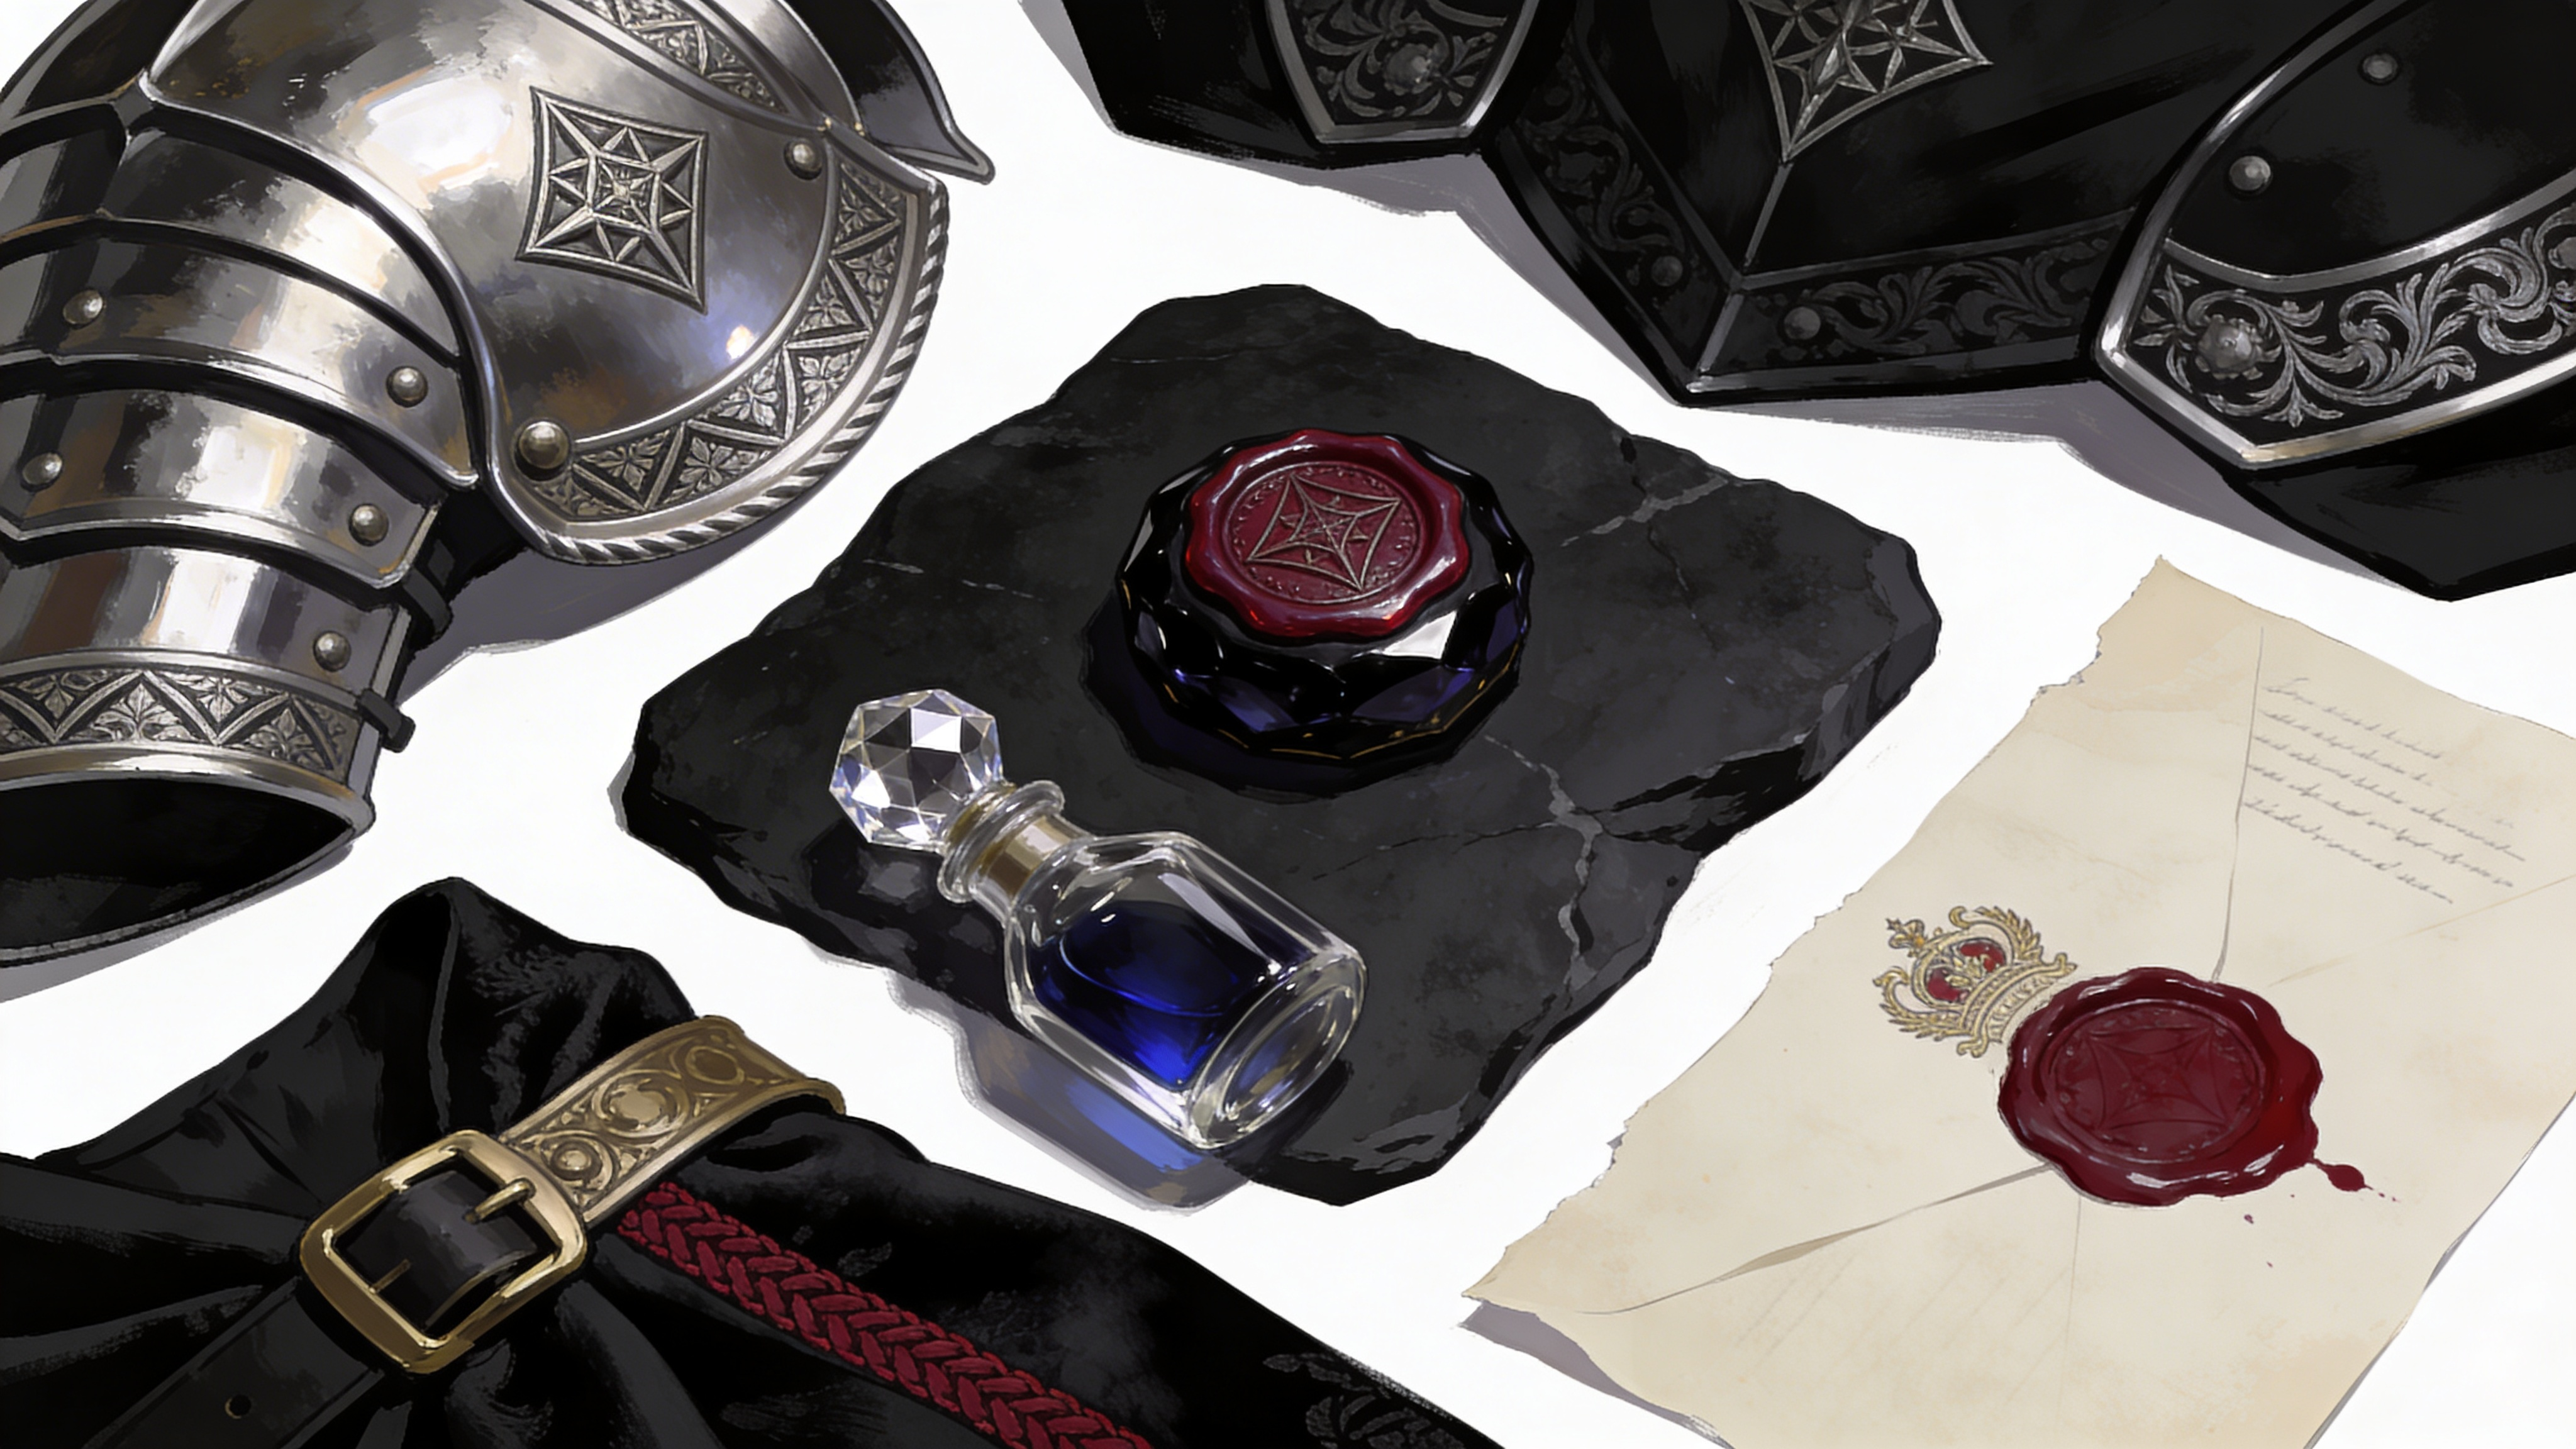
\includegraphics[keepaspectratio,alt={Krone --- Materialpalette: Titanrüstung, Obsidian-Intarsien, Blutrot-Signet, Damaszener-Stahl}]{../concepts/day02-vera/factions/fraktion-krone-materialpalette_seedream-4-5.png}}
\caption{Krone --- Materialpalette: Titanrüstung, Obsidian-Intarsien,
Blutrot-Signet, Damaszener-Stahl}
\end{figure}

\textbf{Architektur der Krone:} - Massives Gestein --- Stampflehm und
Kalkstein in brutalisierten Blöcken - Keine Ornamentik außer
Wappenzeichen - Cantilevierte Plattformen --- Macht durch
Ingenieurleistung demonstriert - Crystal-Glas-Lichtschächte als
architektonisches Statement (Licht von oben als Herrschaftssymbol)

\textbf{Silhouette-Regel:} Kronensoldaten müssen auf 50m von Ordensboten
unterscheidbar sein → Kronenarmour hat breitere Schulterplatten, kürzere
Silhouette, kein weißer Stoff sichtbar.

\begin{center}\rule{0.5\linewidth}{0.5pt}\end{center}

\subsubsection{5.2.2 Der Orden --- Kosmologie des
Wissens}\label{der-orden-kosmologie-des-wissens}

Der Orden kontrolliert Bildung und Inquisition. Seine Materialsprache
ist Reinheit als Drohung: Weiß, das kein Fleck toleriert, ist eine
politische Aussage.

\textbf{Palette:} All-White / Hellgrau mit EIN blassgrünem
Lumineszenz-Akzent. Silberne Präzisions-Details.

\textbf{Materialien Oberschicht:} - Gebleichtes schweres Leinentuch
(geometrisch präzise Stickerei, silberner Faden) -
Kristallglas-Optiklinsen in Messingfassungen (Bildungsmonopol
visualisiert) - Vellum-Manuskriptseiten mit dichter Schrift - Blassgrüne
Alchemie-Phiolen (das einzige Farbsignal --- Wissen als leuchtendes
Gift) - Knochen-Rosenkranz mit schwarzem Obsidian-Mittelelement
(einziger Dunkelakzent)

\begin{figure}
\centering
\pandocbounded{
\includegraphics[keepaspectratio,alt={Orden --- Materialpalette: Weißes Leinengewand, Kristalllinse, Vellum-Manuskript, grüne Alchemiephiole}]{../concepts/day02-vera/factions/fraktion-orden-materialpalette_seedream-4-5.png}}
\caption{Orden --- Materialpalette: Weißes Leinengewand, Kristalllinse,
Vellum-Manuskript, grüne Alchemiephiole}
\end{figure}

\textbf{Architektur des Ordens:} - Romanische Elemente: Rundbögen, dicke
Mauern, Krypta-Gewölbe - Helle, geschliffene Kalkstein-Oberflächen
(Reinheit durch Material) - Schmale Schlitzfenster --- kontrollierte
Lichtmenge als Machtgeste - Bibliotheken in Turmform --- vertikale
Wissenshoheit

\textbf{Silhouette-Regel:} Ordensboten haben hochgeschlossene schmale
Silhouette, weißer Umhang, kein Metall sichtbar. Gegenpol zur massiven
Kronen-Armour.

\begin{center}\rule{0.5\linewidth}{0.5pt}\end{center}

\subsubsection{5.2.3 Die Gilden --- Ontologie des
Materials}\label{die-gilden-ontologie-des-materials}

Die Gilden kontrollieren Produktion und Handel. Ihre Materialsprache ist
akkumulierter Reichtum: Jedes Objekt hat einen Preis, und der ist
signifikant.

\textbf{Palette:} Tiefbraun, Warmambber, Mitternachtsindigo,
Malachitgrün --- mit poliertem Bronze und Gold als Akzente.

\textbf{Materialien Mittelschicht/Oberschicht:} - Schwere Brokatseide in
Nachtindigo mit gewebter Gold-Borte - Polierter
Malachit-Cabochon-Anhänger (Handelsstatus-Signal) -
Bernstein-Perlenreihe (organisch, aber wertvoll) - Bronzehammer auf
Dunkelstein (Werkzeug als Statussymbol) - Vegetabil gegerbtes
Sattlerleder mit geometrischen Blindprägungen - Keramiktiegel mit
Kupferpatina, kleine Glasphiolen mit Pigmenten (Produktionskontrolle)

\begin{figure}
\centering
\pandocbounded{\includegraphics[keepaspectratio,alt={Gilden --- Materialpalette: Indigoseide, Malachit-Anhänger, Bernsteinkette, Bronzewerkzeug, Sattlerleder}]{../concepts/day03-vera/factions/fraktion-gilden-materialpalette-v2_nano-banana-2.png}}
\caption{Gilden --- Materialpalette: Indigoseide, Malachit-Anhänger,
Bernsteinkette, Bronzewerkzeug, Sattlerleder}
\end{figure}

\textbf{Architektur der Gilden:} - Bauhaus-Inspiration: klare Linien,
Funktionalität als Ästhetik - Integrierte Werkstätten im Erdgeschoss
(Produktion als Fassade sichtbar) - Bronzebeschläge und Metallintarsien
an Sandstein-Fassaden - Zunftzeichen in Stein gemeißelt --- Heraldik als
Identitätspolitik - Modulare Fassaden: Erweiterungen wenn Gilde wächst,
Schrumpfungen wenn sie fällt

\textbf{Silhouette-Regel:} Gildenmeister haben breiten Stand,
Lederschürze oder schweres Brokattuch, Werkzeughalter sichtbar.
Mittelklasse-Silhouette --- nicht so schlank wie Krone, nicht so ärmlich
wie Unterschicht.

\begin{center}\rule{0.5\linewidth}{0.5pt}\end{center}

\subsection{5.3 Architektur-Designsprache --- Die vier Schichten
Schwarzrands}\label{architektur-designsprache-die-vier-schichten-schwarzrands}

Schwarzrand ist eine gerichtete Stadt. Sie orientiert sich zur Schwelle
hin --- die Architektur schwillt, lehnt und greift in Richtung des
Abgrunds. Das ist kein Fehler der Stadtplanung. Es ist die physische
Manifestation einer Zivilisation, die ihre Existenz auf einer
kosmologischen Dünnstelle errichtet hat.

\begin{figure}
\centering
\pandocbounded{\includegraphics[keepaspectratio,alt={Schwarzrand --- Kanalzone: Marktquai am Kanal, vertikale Stadtschichten im Hintergrund}]{../concepts/day04-vera/environments/stadtschnitt-kanalzone-v3-final_gpt-image-1-5.png}}
\caption{Schwarzrand --- Kanalzone: Marktquai am Kanal, vertikale
Stadtschichten im Hintergrund}
\end{figure}

\subsubsection{Schicht 1 --- Slums (Untergrund,
Schwellenähe)}\label{schicht-1-slums-untergrund-schwellenuxe4he}

Physik: Schwelle am nächsten. Realität porös. Biolumineszenz überall.

\begin{itemize}
\tightlist
\item
  \textbf{Material:} Gestohlene Ziegel, Holzreste, Lappen als
  Trennwände. Knochen-Schnitzereien.
\item
  \textbf{Licht:} Einzige Lichtquelle: biolumineszente organische
  Ablagerungen in Mörtelfugen --- grünlich, schwach, unzuverlässig.
\item
  \textbf{Atmosphäre:} Deckenhöhe unter 2 Meter. Tunnel, keine Straßen.
  Alles riecht nach feuchtem Stein.
\item
  \textbf{Bewohner:} Schattenfieber-Opfer, illegale Alchemisten,
  Schwarzmarkt-Händler, Kinder der Armen.
\end{itemize}

\textbf{Designregel:} Slums dürfen NICHT pittoresk sein. Kein
romantisierter Armuts-Aesthetic. Wenn es schön ist, ist es bedrohlich
schön --- weil die Biolumineszenz das Fieber signalisiert.

\subsubsection{Schicht 2 --- Mittelstadt (Fachwerk und
Romanik)}\label{schicht-2-mittelstadt-fachwerk-und-romanik}

Historisches Herzstück: fränkische Fachwerkhäuser über romanischen
Kellergewölben.

\begin{itemize}
\tightlist
\item
  \textbf{Material:} Fachwerk aus Eiche, Sandstein für Fundamente und
  Gewölbe. Warmamberfarbenes Talgkerzenlicht.
\item
  \textbf{Licht:} Kleine Fenster mit einfachen Glasscheiben (Buntglas
  nur in Zunfthäusern). Laternen mit Tiertalg.
\item
  \textbf{Atmosphäre:} Laut, eng, lebendig. Märktreiben, Werkstattlärm,
  Stiefelgeräusch auf Kopfsteinpflaster.
\item
  \textbf{Hybridzonen:} An den Rändern zu Schicht 3 ---
  Edelstahlbeschläge am Fachwerk, Bauhaus-Fensterrahmen in romanischen
  Bögen. Die Mittelschicht will aufsteigen und zeigt es.
\item
  \textbf{Kanalzone:} Der Kanal schneidet durch Schicht 2 ---
  Handelsader und Geruchskanal zugleich. Quais als informeller Markt.
\end{itemize}

\textbf{Designregel:} Hier ist die meiste spielerische Zeit. Lesbar,
lebendig, nicht monoton --- jede Gasse hat eine andere Gilde, jede
Fassade ist ein anderer Zunftcharakter.

\subsubsection{Schicht 3 --- Gilden- und Ordensdistrikte
(Brutalistisch/Bauhaus)}\label{schicht-3-gilden--und-ordensdistrikte-brutalistischbauhaus}

Machtarchitektur als Einschüchterung.

\begin{itemize}
\tightlist
\item
  \textbf{Material:} Geschlagener Kalkstein und Stampflehm. Geometrische
  Formen. Metallintarsien in Böden und Fassaden.
\item
  \textbf{Licht:} Polierte Oberflächen reflektieren indirektes Licht ---
  nie direkte Flamme. Eiskaltes weißes Licht.
\item
  \textbf{Atmosphäre:} Still. Weiträumige Plätze, keine Marktstände.
  Wachen alle zwanzig Meter.
\item
  \textbf{Gildenhallen:} Offen nach vorn (Produktion sichtbar --- Macht
  durch Transparenz). Türme als Signet.
\item
  \textbf{Ordensbibliotheken:} Geschlossen, keine Fenster nach unten,
  schmale Schlitzfenster nach oben.
\end{itemize}

\textbf{Designregel:} Hier wirkt der Spieler klein. Gebäude sind
mindestens dreimal menschliche Höhe. Plätze haben keine schützenden
Ecken. Das ist beabsichtigt --- Kontrollarchitektur.

\subsubsection{Schicht 4 --- Kronenfestung (Geometrischer
Brutalismus)}\label{schicht-4-kronenfestung-geometrischer-brutalismus}

Das absolute Oben. Hier endet die Hierarchie.

\begin{itemize}
\tightlist
\item
  \textbf{Material:} Reiner geometrischer Stein. Kein Ornament.
  Cantilevierte Plattformen über dem Abgrund.
\item
  \textbf{Licht:} Tageslicht durch Kristallglas-Lichtschächte. Licht als
  Privilege --- je höher, desto mehr Sonne.
\item
  \textbf{Atmosphäre:} Windgepeitschte Terrassen. Hängende Gärten am
  Rand des Nichts. Schweigen.
\item
  \textbf{Richtungsgeste:} Die Kronenfestung lehnt am weitesten in
  Richtung Schwelle. Der König kennt die Gefahr und steht dennoch am
  nächsten --- das ist der Beweis seiner Legitimation.
\end{itemize}

\textbf{Designregel:} Keine natürliche Vegetation außer den Hängegärten.
Kein Lärm. Ein Spieler, der hier steht, ist entweder mächtig oder in
extremer Gefahr.

\begin{center}\rule{0.5\linewidth}{0.5pt}\end{center}

\subsection{5.4
Charakter-Design-Prinzipien}\label{charakter-design-prinzipien}

\subsubsection{5.4.1 Hauptprinzip: Comme des Garçons trifft
mittelalterliche
Rüstung}\label{hauptprinzip-comme-des-garuxe7ons-trifft-mittelalterliche-ruxfcstung}

Silhouetten sind tailored, körperbetont, geschichtet. Kein Übergewicht
an Schmuck. Jedes Detail hat Funktion.

\textbf{Schichtung (für alle Charaktere):} 1. Grundlage: Gambeson
(Steppstoff) oder einfaches Leinengewand 2. Mittelschicht:
Kettenhemd-Segmente oder geschnürtes Leder 3. Außenschicht:
Platten-Elemente (nicht vollständig --- Beweglichkeit bleibt sichtbar)

\textbf{Oberfläche:} - Gebürstetes Metall, nicht poliert (außer
Krone-Eliten: poliert als Statussignal) - Geätzte Ornamente und
Nieten-Muster (nicht dekorativ, sondern Marker) - Patina an Kanten
(Alter und Gebrauch sind Würde)

\textbf{Akzente (nach Fraktion):} - Krone: Blutrot-Email,
Goldfaden-Stickerei minimal, schwarzes Brokattuch - Orden:
Silber-Stickerei, Knochendetails, weißes Leinengewebe - Gilden:
Bernstein-Einlagen, Malachit-Applikationen, Lederpunzierungen

\textbf{Asymmetrie als Prinzip:} Avant-garde Silhouetten --- kein
symmetrisches Mittelalterkostüm. Eine Schulter breiter. Eine Seite
Kettenhemd, andere Seite Platte. Das ist das ``High Fashion''-Signal.

\begin{center}\rule{0.5\linewidth}{0.5pt}\end{center}

\subsubsection{5.4.2 Das Tiervolk ---
Design-Prinzipien}\label{das-tiervolk-design-prinzipien}

Das Tiervolk lebt in dauerhafter kosmologischer Symbiose. Das bedeutet:
das Tier ist erkennbar --- es ist ein Fuchs, ein Marder, ein Rabe ---
aber es trägt etwas in sich, das nicht hineingehört. Die Fremdheit ist
nie theatralisch. Sie ist subtil und präzise.

\textbf{Das Kernprinzip: Subtile anatomische Verschiebung}

Das Tiervolk ist NICHT monströs. Es ist leicht falsch. Der visuelle
Unterschied zu einem ``normalen'' anthropomorphen Tier liegt in Details,
die den Spieler verunsichern ohne ihn zu erschrecken:

\begin{itemize}
\tightlist
\item
  \textbf{Augen:} Pupillen stimmen nicht --- vertikal geschlitzt wie
  eine Katze, oder horizontal wie ein Ziege, oder ohne sichtbare Pupille
  mit einer internen Tiefe, als wäre das Licht im Auge gefangen
\item
  \textbf{Fell/Federstruktur:} Wächst an Nacken und Schultern gegen den
  Strich. Erzeugt Konter-Wirbelmuster. Bei Vögeln: sekundäres
  geometrisches Muster unter der natürlichen Federanordnung sichtbar
\item
  \textbf{Proportionen:} Fraktiell verschoben --- Arme minimal zu lang,
  Hals dreht einen Tick zu weit, Finger biegen ein Gelenk zuviel
\item
  \textbf{Schatten:} Fallen nicht ganz richtig (für Concept Art:
  Schattenwinkel ist unabhängig von tatsächlicher Lichtquelle)
\item
  \textbf{Stillstand:} Das Tiervolk steht zu still. Kein Schaukeln, kein
  Blinzeln im normalen Rhythmus. Als würde der Körper auf Befehl ruhen,
  nicht aus Entspannung
\end{itemize}

\textbf{Was das Tiervolk NICHT ist:} - Kein Tribal --- kein
Stammesschmuck, keine Knochenhalsketten, kein Totemismus - Kein Monster
--- keine Deformationen, kein Body-Horror, kein Ekel-Design - Kein
Disney --- keine großen Augen, keine ``cute''-Proportion, keine
Niedlichkeit - Keine Magier --- das Tiervolk ist praktisch, händlerisch,
geerdet in Material

\textbf{Kleidung --- nach Archetyp:}

\emph{Händler:} Zweckmäßig, gut genutzt, nicht arm. Schwerer dunkler
Wollmantel, mehrere Ledertaschen am Gürtel, Schultertasche aus geöltem
Segeltuch, lederbehandelte Hände. Keine Insignien. Farbe: Anthrazit,
Sienna-Brauntöne, ein gedämpfter Indigoakzent --- nie Fraktionsfarben.

\emph{Dieb/Kundschafter:} Eng anliegend, geschichtet, alles Schwarz oder
Aschgrau. Lederstrapping, weiche Sohlen. Kein Metall sichtbar.
Silhouette: schlank, komprimiert, bereit.

\emph{Bote/Informationshändler:} Mehrschichtige Roben, Dokumententasche
aus schwerem Leder, Werkzeuggürtel mit knochengriffigen Instrumenten.
Ein einzelner Farbakzent als Codierung (oxblood-roter Gürtelstrick =
freie Bewegung in allen Distrikten).

\textbf{Farbpalette Tiervolk:} Die Tiervolk-Palette liegt NEBEN den
Fraktionspaletten --- weder Krone noch Orden noch Gilden. Das ist
Absicht: Tiervolk ist fraktionslos. - Anthrazit, Kohleschwarz, Aschgrau
(Kleidung) - Warmes Sienna, sandigeres Braun, gedämpftes Ochre
(Fell/Federfarben) - Maximal EIN Akzent, gedämpft --- kein
Fraktionssignal

\textbf{Konzept-Bildmaterial --- Tiervolk:}

\begin{figure}
\centering
\pandocbounded{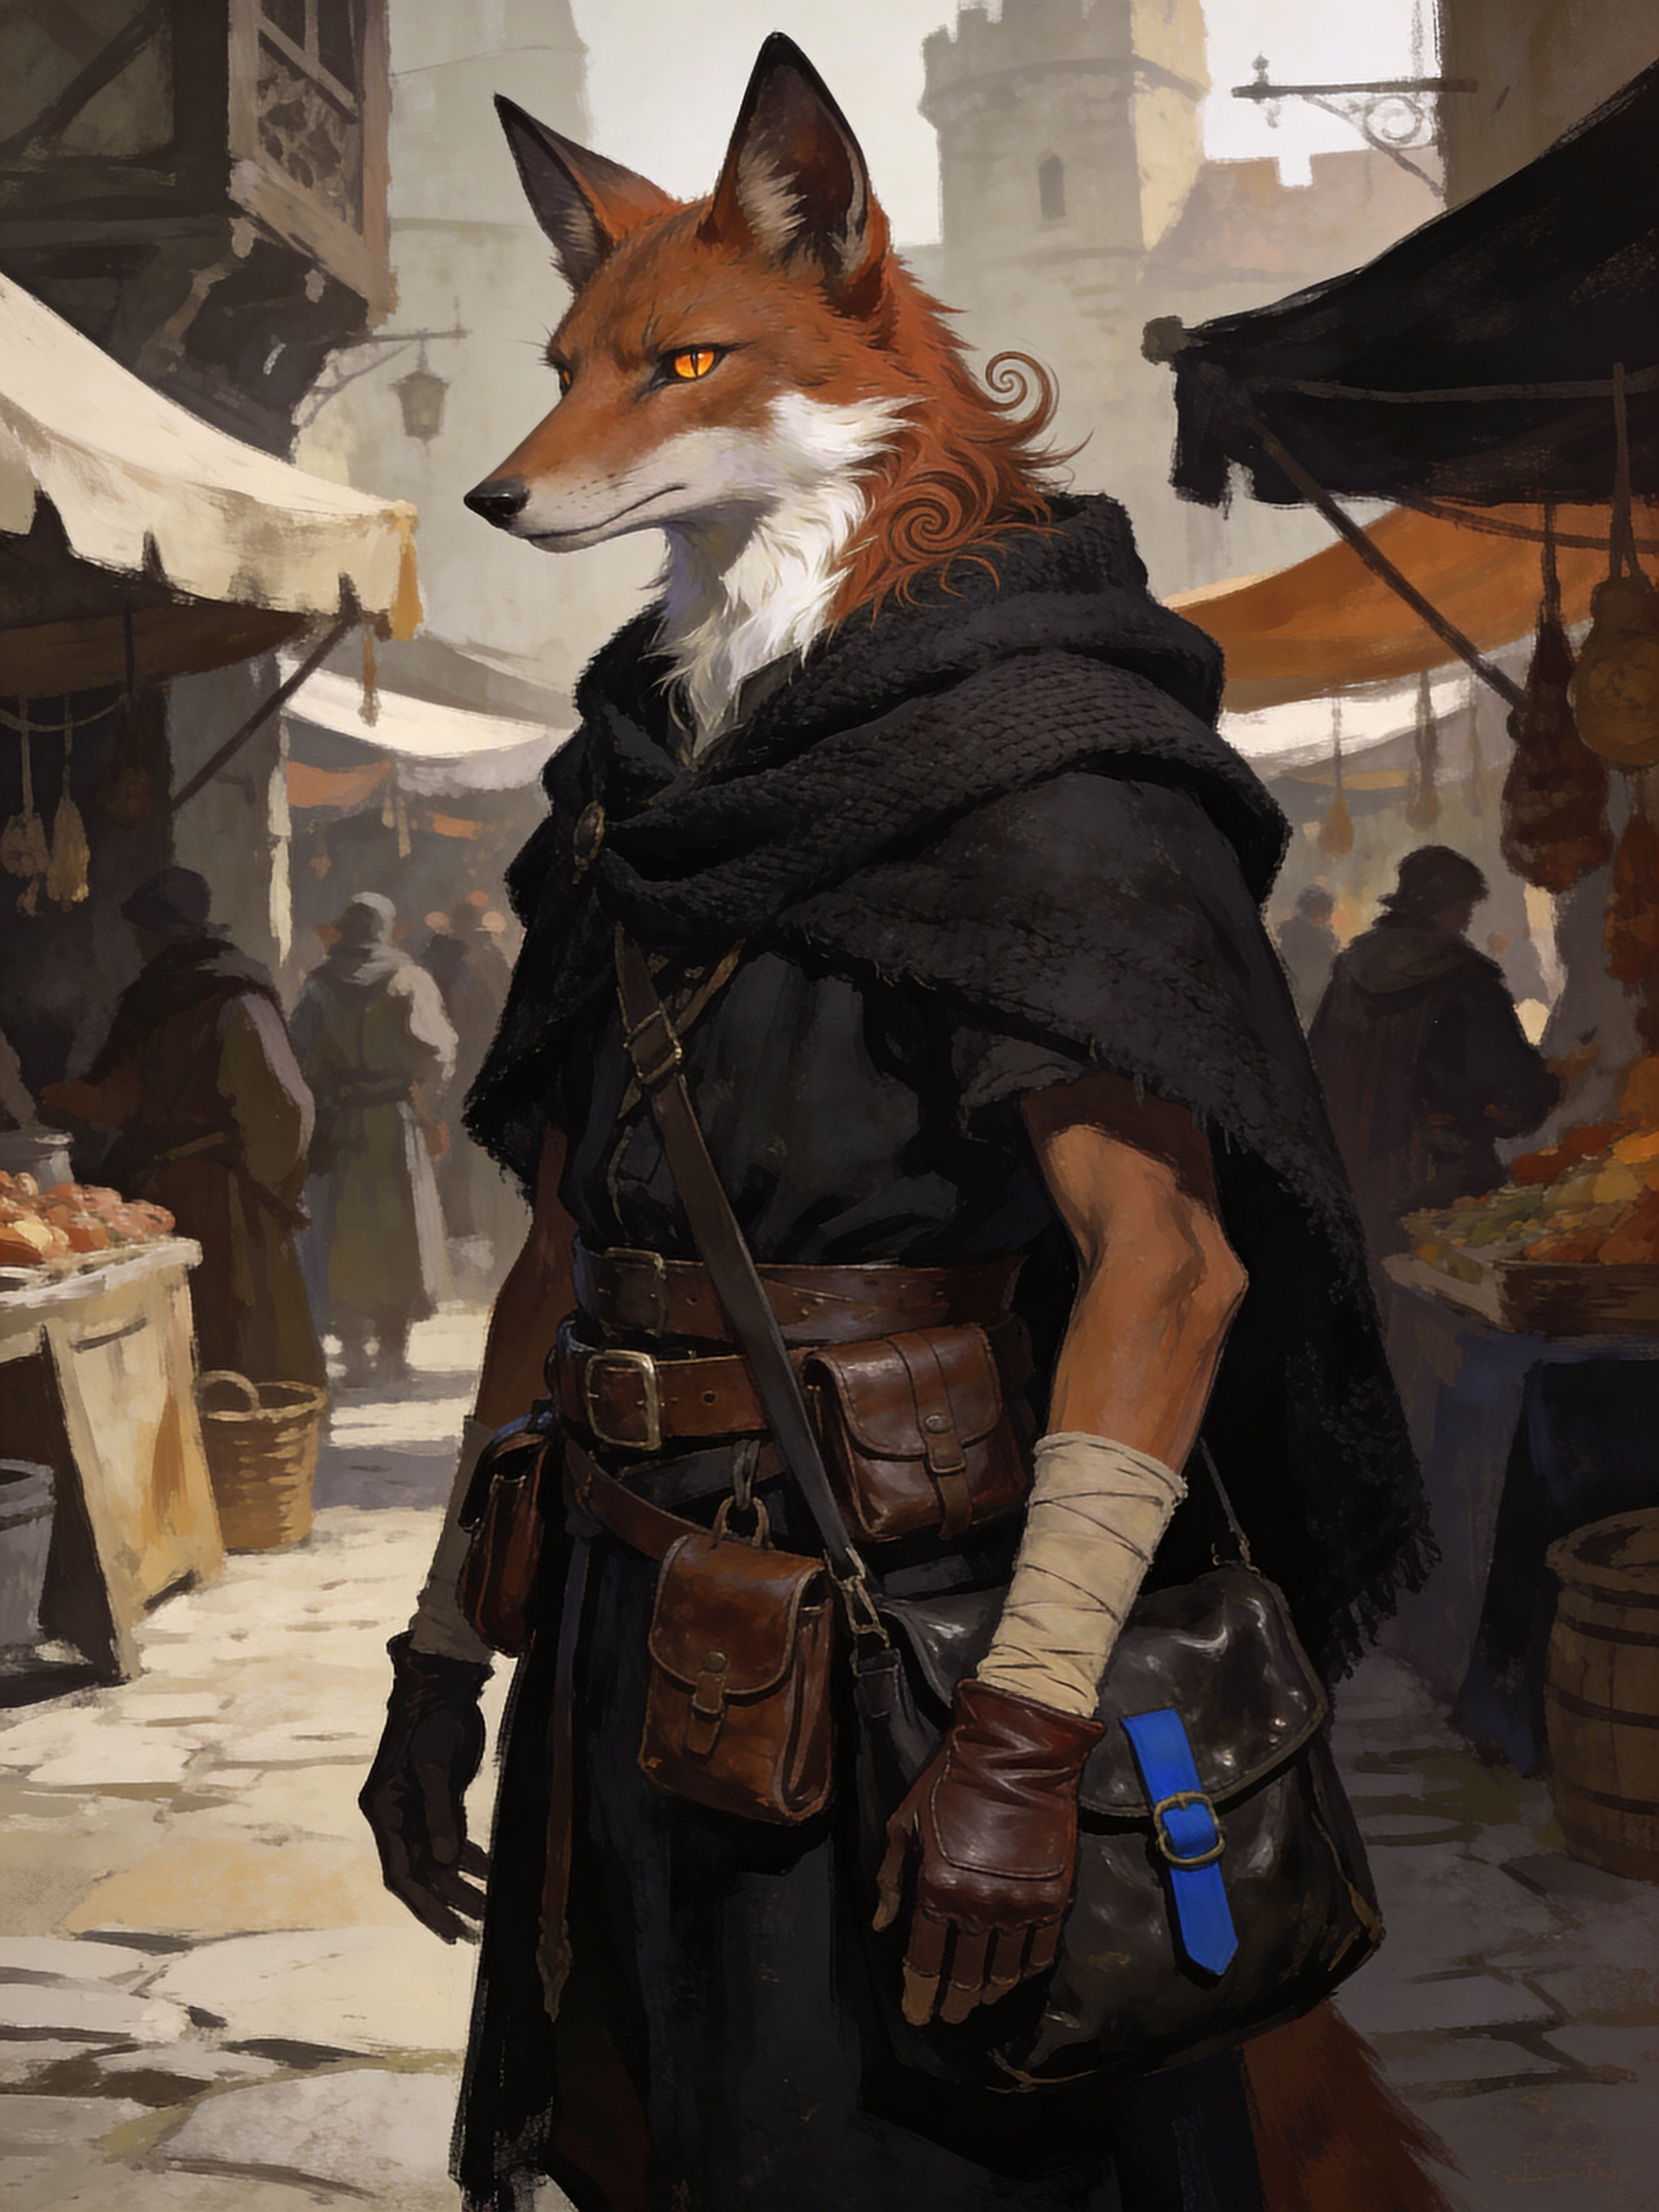
\includegraphics[keepaspectratio,alt={Tiervolk --- Händler Fuchs: Aufrechte Fuchsfigur im Marktkontext, Händler-Silhouette, subtile Fremdheit}]{../concepts/day04-vera/tiervolk/tiervolk-haendler-fuchs-exploration_seedream-4-5.png}}
\caption{Tiervolk --- Händler Fuchs: Aufrechte Fuchsfigur im
Marktkontext, Händler-Silhouette, subtile Fremdheit}
\end{figure}

\begin{figure}
\centering
\pandocbounded{
\includegraphics[keepaspectratio,alt={Tiervolk --- Diebin Marder: Schlanke Marderfigur auf Dachvorsprung, Dieb-Silhouette, Augen leuchten foxfire-grün}]{../concepts/day04-vera/tiervolk/tiervolk-diebin-marder-exploration_seedream-4-5.png}}
\caption{Tiervolk --- Diebin Marder: Schlanke Marderfigur auf
Dachvorsprung, Dieb-Silhouette, Augen leuchten foxfire-grün}
\end{figure}

\begin{figure}
\centering
\pandocbounded{
\includegraphics[keepaspectratio,alt={Tiervolk --- Rabe-Bote: Rabenhumanoid im Steinbogen, Dokumentenbote, oxblood-Gürtel als Codierung}]{../concepts/day04-vera/tiervolk/tiervolk-rabe-bote-exploration_seedream-4-5.png}}
\caption{Tiervolk --- Rabe-Bote: Rabenhumanoid im Steinbogen,
Dokumentenbote, oxblood-Gürtel als Codierung}
\end{figure}

\begin{figure}
\centering
\pandocbounded{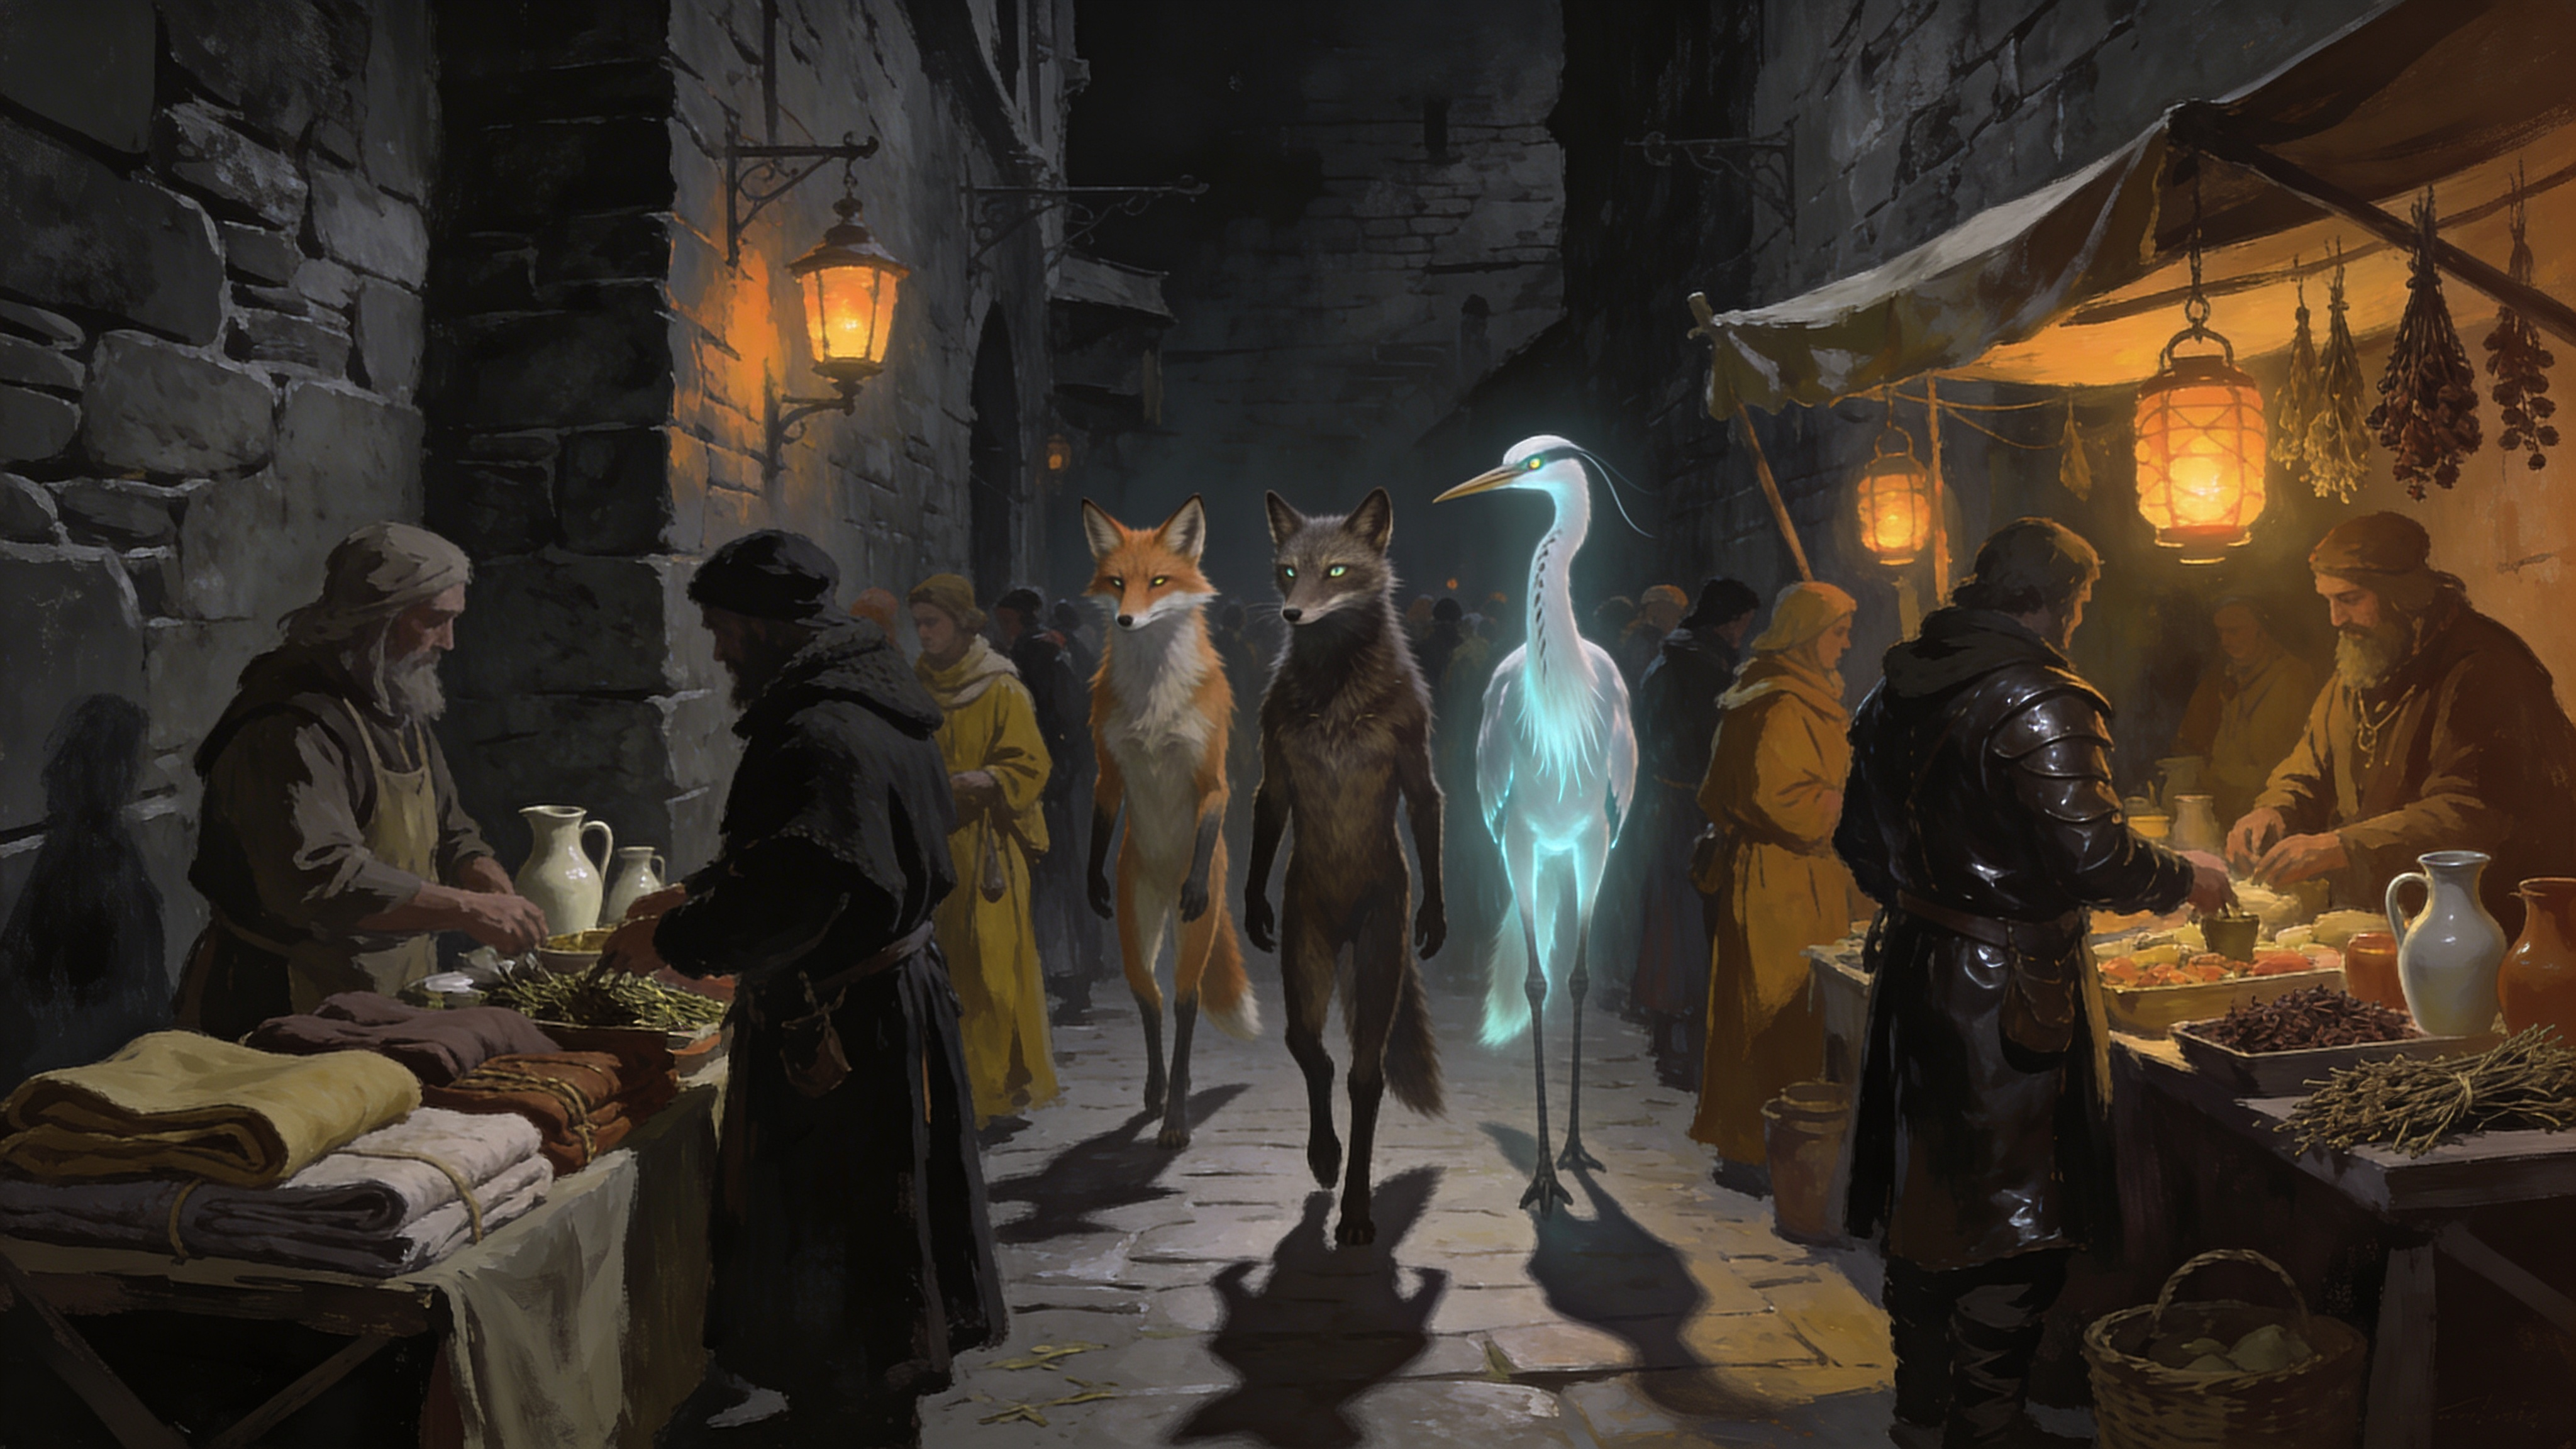
\includegraphics[keepaspectratio,alt={Tiervolk --- Marktszene: Fuchs und Reiher unter Menschenmenge, integriert aber subtil anders}]{../concepts/day04-vera/tiervolk/tiervolk-marktszene-exploration_seedream-4-5.png}}
\caption{Tiervolk --- Marktszene: Fuchs und Reiher unter Menschenmenge,
integriert aber subtil anders}
\end{figure}

\begin{figure}
\centering
\pandocbounded{\includegraphics[keepaspectratio,alt={Tiervolk --- Hero-Sheet Fuchs: Charakter-Konzept mit Detailinsets, Symbiose-Zeichen erkennbar}]{../concepts/day04-vera/tiervolk/tiervolk-hero-symbiose_nano-banana-pro.png}}
\caption{Tiervolk --- Hero-Sheet Fuchs: Charakter-Konzept mit
Detailinsets, Symbiose-Zeichen erkennbar}
\end{figure}

\begin{center}\rule{0.5\linewidth}{0.5pt}\end{center}

\subsection{5.5 Relikt --- Der
Schwellenanker}\label{relikt-der-schwellenanker}

\subsubsection{5.5.1 Formsprache}\label{formsprache}

Der Schwellenanker ist eine \textbf{komprimierte gefaltete geologische
Formation} --- nicht Knochen, nicht Kristall, nicht Werkzeug. Er ist zu
regelmäßig für Zufall, zu organisch für Handwerk. Entstanden durch
Jahrtausende von Schwelle-Einwirkung auf Mineral.

\textbf{Form-Deskription:} Fistgroße Knollen-Masse. Sedimentgestein, das
in sich gefaltet und unter extremem Druck komprimiert wurde. Oberfläche:
dichtes Netz von osszifizierten Mikro-Kanälen, die durch kalzifizierte
organische Matrix verlaufen. Die Kanäle sind das visuelle Key-Feature
--- sie verraten den Schwellenanker, wenn alles andere ihn als normalen
Stein erscheinen lässt.

\textbf{Was er NICHT ist:} - Kein Wirbelsäulenknochen (abgewiesen:
Briefing-Entscheidung, kein anatomisches Artefakt) - Kein Kristall (zu
clean, zu ordentlich --- Kristall impliziert Wachstum, Schwellenanker
impliziert Kompression) - Kein Schmuckstück (keine Fassung, keine
Politur, kein Design-Eingriff)

\subsubsection{5.5.2 Drei Zustände}\label{drei-zustuxe4nde}

Die Dramaturgie des Schwellenankern wird visuell über drei Zustände
erzählt. Diese Zustände sind Gameplay-Information --- der Spieler lernt,
sie zu lesen.

\begin{figure}
\centering
\pandocbounded{\includegraphics[keepaspectratio,alt={Schwellenanker --- Drei Zustände: Ruhend \textbar{} Aktiviert \textbar{} Auflösung}]{../concepts/day03-vera/relics/relikt-drei-zustaende-v2_nano-banana-pro.png}}
\caption{Schwellenanker --- Drei Zustände: Ruhend \textbar{} Aktiviert
\textbar{} Auflösung}
\end{figure}

\textbf{Zustand Null --- Ruhend:} Aschgrau. Kein Glanz, kein Licht. Die
Mikro-Kanäle sind leer --- dunkel, trocken, unremarkable. Auf 10 Meter
Entfernung: ein Stein. Nur bei direkter Betrachtung verrät das
pathologische Regelmäßigkeit der Kanäle etwas Außergewöhnliches.

\emph{Spieler-Lesbarkeit:} Das Relikt ist inaktiv. Kein Effekt, keine
Reaktion, keine Interaktion möglich.

\textbf{Zustand Eins --- Aktiviert:} Biolumineszenz von innen. Pale
Blue-Violett füllt die Mikro-Kanäle wie phosphoreszierende Flüssigkeit
in einem Kreislaufsystem. Der Glanz diffus, von innen heraus --- nicht
von der Oberfläche. Schön. Tief unsettling.

\emph{Spieler-Lesbarkeit:} Das Relikt resoniert.
Schwellenfieber-Empfindlichkeit maximal. Gameplay: besondere Fähigkeiten
aktiv, aber Lymph-System unter Belastung.

\textbf{Zustand Drei --- Auflösung:} Ränder evaporieren als feines
mineralisches Partikelstaub. Inneres Leuchten: überhell und hässlich ---
übersteuert, kränklich Gelbgrün an den aufbrechenden Kanalrändern. Das
Schöne ist weg. Die Formation verliert Kohärenz.

\emph{Spieler-Lesbarkeit:} Kritischer Zustand. Weiterführung verursacht
irreversible Schwelle-Kontamination. Abort or continue --- das ist die
Spielerentscheidung.

\subsubsection{5.5.3 Hero-Shot}\label{hero-shot}

Der Schwellenanker in seiner atmosphärischen Präsentation: auf einem
Altar in einem Gewölberaum, als einzige Lichtquelle. Die Spielerfigur am
Bildrand, klein, awed.

\begin{figure}
\centering
\pandocbounded{\includegraphics[keepaspectratio,alt={Schwellenanker --- Hero-Shot v2: Geologische Formation auf Altar, Gewölbekrypta, Figur am Rand}]{../concepts/day04-vera/relics/relikt-hero-v2_nano-banana-pro.png}}
\caption{Schwellenanker --- Hero-Shot v2: Geologische Formation auf
Altar, Gewölbekrypta, Figur am Rand}
\end{figure}

\begin{center}\rule{0.5\linewidth}{0.5pt}\end{center}

\subsection{5.6 Schattenfieber --- Visuelle
Progression}\label{schattenfieber-visuelle-progression}

Das Schattenfieber ist biologisch. Seine visuelle Progression zeigt
diesen biologischen Charakter: keine magische Aura, keine
Spektral-Effekte, keine leuchtenden Augen. Das Fieber verändert den
Körper von innen.

\subsubsection{Stufe 1 --- Sensorisch
(reversibel)}\label{stufe-1-sensorisch-reversibel}

\textbf{Sichtbares Zeichen:} Hauchfeine Blutgefäß-Linien unter der Haut,
vor allem an Handgelenken und Halsansatz. Kaum sichtbar --- nur bei
direktem Licht und naher Distanz.

\textbf{Farbe:} Blassviolett, exakt so wie der aktivierte
Schwellenanker. Das ist kein Zufall.

\textbf{Design-Regel:} In Stufe 1 wirkt der Charakter nicht ``krank.''
Er wirkt interessant. Fast schön. Das ist die Falle.

\subsubsection{Stufe 2 --- Mutativ
(managebar)}\label{stufe-2-mutativ-managebar}

\textbf{Sichtbares Zeichen:} Gefäßlinien jetzt deutlich --- treten aus
der Haut hervor als leicht erhabene Kanäle. Hautton drumherum verschoben
(grauer, kühler).

\textbf{Biotech-Konsequenz:} In dieser Stufe ist Schattenfieber
spielbar. Die Gefäßlinien leiten Energie. Spezialfähigkeiten werden
möglich --- mit Körperkosten.

\textbf{Design-Regel:} Schicht-2-Charaktere mit Schattenfieber sind im
Spiel sichtbar. Kein Stigma-Klischee --- Fieber ist manchmal Macht. Der
moralische Preis ist nicht der Körper, sondern das, was man für den
Körper tut.

\subsubsection{Stufe 3 --- Auflösung
(irreversibel)}\label{stufe-3-aufluxf6sung-irreversibel}

\textbf{Sichtbares Zeichen:} Material-Transition. Haut wird transluzent.
Darunter: die Gefäßlinien leuchten kränklich gelbgrün --- identische
Farbverschiebung wie Schwellenanker-Zustand-Drei. Die Person evaporiert
an den Rändern.

\textbf{Design-Regel:} Stufe-3-Charaktere sind selten im Spiel sichtbar.
Wenn, dann immer isoliert, immer traurig, nie als Bedrohung. Sie sind
Warnung, nicht Monster.

\subsubsection{Schattenfieber und das
Tiervolk}\label{schattenfieber-und-das-tiervolk}

Das Tiervolk trägt die Symbiose in sich --- aber ob das Schattenfieber
und die kosmologische Symbiose des Tiervolks dieselbe Wurzel haben, ist
eine offene Lore-Frage. Visuell: die Tiervolk-Anomalien (Augen,
Fell-Gegenrichtung, Gelenke) sind KEINE Schattenfieber-Zeichen. Sie sind
stabil, kongenital, nicht progressiv. Das ist der entscheidende visuelle
Unterschied: Schattenfieber schreitet fort. Die Tiervolk-Fremdheit
verändert sich nicht.

\subsubsection{UI-Korrespondenz}\label{ui-korrespondenz}

Die Levelingsicht (halbtransparentes Nervensystem --- Cardio / Muskel /
Lymph) entspricht direkt der Schattenfieber-Visualisierung. Das
Lymph-Subsystem leuchtet blassviolett wenn das Fieber aktiv ist. Je
stärker das Leuchten, desto näher Stufe 2.

\textbf{Warum das funktioniert:} Der Spieler trägt das
Schattenfieber-System buchstäblich im Körper. Die Schwelle ist nicht
außen. Sie ist innen. Das ist das Gefühl, das RELICS erzeugen soll.

\begin{center}\rule{0.5\linewidth}{0.5pt}\end{center}

\subsection{5.7 Referenz-Kanon}\label{referenz-kanon}

\subsubsection{Primäre Referenzen}\label{primuxe4re-referenzen}

\textbf{Dark Souls / Elden Ring:} - Licht aus dem Körper heraus, nicht
von oben - Architektur als emotionaler Raum - 50-Meter-Silhouette-Regel
konsequent angewendet - Dunkel als Normalzustand (Licht ist Privileg,
nicht Default)

\textbf{Control (Remedy):} - Brutalismus als emotionale Raumsprache -
Das Unheimliche durch geometrische Perfektion erzeugen - Material als
Machtträger

\textbf{Hollow Knight:} - Vertikalität als Weltstruktur - Biolumineszenz
in Dunkel als primäre visuelle Sprache - Größenverhältnisse als
emotionale Aussage

\textbf{Dishonored:} - Sozialer Status durch visuelle Schichtung immer
sichtbar - Vertikalität im Level-Design: Dächer als separate
Gesellschaft - Materialsprache für Klassen konsequent getrennt

\subsubsection{Architektur-Referenzen}\label{architektur-referenzen}

\textbf{Gaudi:} Organisch-strukturelle Formen. Biolumineszenz-Kanäle
folgen dieser Logik --- Struktur und Ornament sind dasselbe.

\textbf{Le Corbusier / Bauhaus:} Gilden-Architektur. Funktion als
Ästhetik. Das Werkzeug IS das Design.

\textbf{Brutalismus (Smithson, Lasdun):} Krone-Festung und
Ordensgebäude. Macht durch Masse. Einschüchterung durch Geometrie.

\subsubsection{Anti-Referenzen (was wir nicht
machen)}\label{anti-referenzen-was-wir-nicht-machen}

\begin{itemize}
\tightlist
\item
  \textbf{World of Warcraft:} Übergesättigte Farben, lesbares
  Fraktionssystem durch bunte Plakate. Das Gegenteil von RELICS.
\item
  \textbf{Generic Fantasy Stock:} Braune Schmutzoptik ohne Designwillen.
  RELICS ist Schmutz MIT Designwillen.
\item
  \textbf{Steampunk-Ornamentik:} Zahnräder als Dekoration. Bei uns sind
  Zahnräder, wenn überhaupt vorhanden, versteckt in Mechanismen.
\item
  \textbf{Furry-Ästhetik:} Das Tiervolk hat nichts mit Furry-Design zu
  tun. Kein Softfocus-Fell, keine großen Augen, keine Liebenswürdigkeit.
  Das Tiervolk ist befremdlich.
\end{itemize}

\begin{center}\rule{0.5\linewidth}{0.5pt}\end{center}

\subsection{5.8 Art Direction-Checkliste (für alle
Assets)}\label{art-direction-checkliste-fuxfcr-alle-assets}

Jedes Asset (Umgebung, Charakter, UI, Effekt) muss gegen diese Liste
geprüft werden:

\begin{itemize}
\tightlist
\item[$\square$]
  \textbf{Fraktion lesbar?} --- Welche Fraktion ``spricht'' dieses
  Asset? Auch neutrale Assets brauchen eine soziale Verortung.
\item[$\square$]
  \textbf{Schicht lesbar?} --- Oberschicht, Mittelschicht oder
  Unterschicht? Materialien müssen eindeutig sein.
\item[$\square$]
  \textbf{50-Meter-Silhouette?} --- Ist das auf Distanz lesbar?
\item[$\square$]
  \textbf{Farbpalette korrekt?} --- Dominante Neutralfarbe + maximal EIN
  kräftiger Akzent.
\item[$\square$]
  \textbf{Keine verbotenen Elemente?} --- Kein Hexagon, kein Zahnrad,
  kein Dampf, kein Sci-Fi-Material.
\item[$\square$]
  \textbf{Materiallogik stimmt?} --- Passt das Material zum Wohlstand
  der Figur/des Ortes?
\item[$\square$]
  \textbf{Schattenfieber berücksichtigt?} --- Bei relevanten
  Charakteren/Orten: Blassviolett-Kanäle sichtbar?
\item[$\square$]
  \textbf{Licht als Privilege?} --- Wer hat Zugang zu guter Beleuchtung?
  Zeigt das Asset das?
\item[$\square$]
  \textbf{Tiervolk-Test (nur Tiervolk-Assets):} Ist die Fremdheit subtil
  (nicht monströs)? Ist kein Tribal-Design sichtbar? Ist die
  Fraktionslosigkeit erkennbar?
\end{itemize}

\begin{center}\rule{0.5\linewidth}{0.5pt}\end{center}

\clearpage

\section{GDD Kapitel 6: Technische Spezifikation \&
Produktion}\label{gdd-kapitel-6-technische-spezifikation-produktion}

\textbf{RELICS: Schwellenanker}

\begin{center}\rule{0.5\linewidth}{0.5pt}\end{center}

\begin{quote}
\textbf{Anmerkung zur Dokumentstruktur} Dieses Kapitel ist die
technische Antwort auf das kreative Briefing. Jede Entscheidung hier hat
einen Grund --- und den schreibe ich dazu. Wenn eine Entscheidung keine
Begründung hat, gehört sie nicht ins Dokument.
\end{quote}

\begin{center}\rule{0.5\linewidth}{0.5pt}\end{center}

\subsection{6.1 Engine \&
Technologiebasis}\label{engine-technologiebasis}

\subsubsection{6.1.1 Unreal Engine 5 ---
Begründung}\label{unreal-engine-5-begruxfcndung}

RELICS wird in \textbf{Unreal Engine 5} entwickelt. Diese Entscheidung
ist gesetzt und nicht diskussionswürdig. Die Begründung:

Das Kernszenario --- eine vertikal geschichtete Stadt mit extremer
Geometriedichte, biolumineszenten Materialien, dynamischer
Globalbeleuchtung und einem Post-Process-System, das die
Spielwahrnehmung schrittweise deformiert --- erfordert eine Kombination
aus Nanite, Lumen und World Partition. Kein anderes aktuell verfügbares
System bietet alle drei in Integration. Custom-Engine-Arbeit wäre für
ein Studio dieser Größe prohibitiv.

\textbf{Engine-Version}: UE5.4 LTS (Long-Term Support Release). Kein
Upgrade während der Alpha-Phase. Feature-Patches werden erst nach Beta
evaluiert.

\textbf{Ziel-Plattform (primär)}: Windows PC (DirectX 12)
\textbf{Ziel-Plattform (sekundär)}: PlayStation 5, Xbox Series X (nach
Full-Release evaluiert)

\textbf{Hardware-Mindestanforderungen (PC, Zielzustand):} \textbar{}
Stufe \textbar{} GPU \textbar{} RAM \textbar{} Einstellung \textbar{}
\textbar---\textbar---\textbar---\textbar---\textbar{} \textbar{}
Minimum \textbar{} NVIDIA RTX 2070 / AMD RX 6700 XT \textbar{} 16 GB
\textbar{} Lumen Software RT, mittlere Qualität \textbar{} \textbar{}
Empfohlen \textbar{} NVIDIA RTX 3080 / AMD RX 7900 XT \textbar{} 32 GB
\textbar{} Lumen Hardware RT, hohe Qualität \textbar{} \textbar{} Ultra
\textbar{} NVIDIA RTX 4080 / AMD RX 7900 XTX \textbar{} 32 GB \textbar{}
Full Hardware RT, maximale Qualität \textbar{}

\emph{Anmerkung}: Die Minimum-Konfiguration nutzt Lumen im
Software-RT-Modus. Das degeneriert GI-Qualität in den Slum-Unterebenen
merklich. Akzeptabel --- die Unterebenen sind dunkel per Design.

\begin{center}\rule{0.5\linewidth}{0.5pt}\end{center}

\subsubsection{6.1.2 Kernkomponenten der
Engine}\label{kernkomponenten-der-engine}

\textbf{Nanite} --- Virtualisierte Geometrie Nanite ist für die gesamte
statische Architekturgeometrie aktiviert. Die Materiallesbarkeit der
Welt --- Zunftzeichen-Reliefs, Titan-Legierung-Oberflächendetail,
Knochen-Schnitzereien der Unterschicht --- funktioniert nur mit
Nanite-Detailauflösung. Ohne LOD-Authoring pro Mesh spart das
konservativ geschätzt 40--60\% des Modellierungs-Aufwands gegenüber
traditioneller Pipeline.

\emph{Bekannte Schwächen und Kompensation:} - \textbf{Dünne Geometrien}
(Ketten, Gitterstäbe, Pflanzenstifte, Stoff-Überhänge): Nanite crasht
bei Meshes unter \textasciitilde2px projected-size. Diese Kategorie
behält traditionelle LODs und Imposter-Billboards ab Distanzklasse 3. -
\textbf{Wasser, Transluzenz}: Nanite unterstützt keine transluzenten
Materialien. Alle Wasseroberflächen und Glas-Elemente sind non-Nanite
mit eigenem LOD-Setup. - \textbf{Moving Meshes}: Nanite funktioniert für
statische und leicht animierte Meshes. Kampf-Props, die zerstört werden
können, müssen als Nanite-Fallback-Mesh mit Destruction-Proxy gebaut
werden.

\begin{center}\rule{0.5\linewidth}{0.5pt}\end{center}

\textbf{Lumen} --- Dynamische Globalbeleuchtung und Reflexionen

Lumen ist das wichtigste und gleichzeitig riskanteste System im Projekt.
Die Begründung ist direkt: eine lebendige, biolumineszente Stadt mit
phosphoreszierenden Mineralien, Alchemie-Lampen und
Schattenfieber-Mutationen braucht echte dynamische GI. Statisches Baked
Lighting würde jeden Runtime-Zustandswechsel --- das Aktivieren des
Schwellenankens, eine Schattenfieber-Eskalation, die
Biolumineszenz-Klasse-A-Emitter --- optisch inkonsistent machen.

\emph{Lumen-Konfiguration nach Stadtschicht:}

{\def\LTcaptype{none} % do not increment counter
\begin{longtable}[]{@{}
  >{\raggedright\arraybackslash}p{(\linewidth - 4\tabcolsep) * \real{0.3333}}
  >{\raggedright\arraybackslash}p{(\linewidth - 4\tabcolsep) * \real{0.3333}}
  >{\raggedright\arraybackslash}p{(\linewidth - 4\tabcolsep) * \real{0.3333}}@{}}
\toprule\noalign{}
\begin{minipage}[b]{\linewidth}\raggedright
Schicht
\end{minipage} & \begin{minipage}[b]{\linewidth}\raggedright
Modus
\end{minipage} & \begin{minipage}[b]{\linewidth}\raggedright
Begründung
\end{minipage} \\
\midrule\noalign{}
\endhead
\bottomrule\noalign{}
\endlastfoot
\textbf{Layer 3} (Türme, Gilden-Hochbau) & Hardware Raytracing & Offener
Himmel, viele Bergkristall-Linsen-Reflektionen --- hier ist
Hardware-RT-Qualität sichtbar und rechtfertigbar \\
\textbf{Layer 2} (Brücken, Arkaden) & Hardware Raytracing & Starke
Buntglas-Farbflecken auf Böden, Reflexionen in Metall-Intarsien --- RT
sichtbar \\
\textbf{Layer 1} (Straßenebene) & Software Raytracing (hohe Qualität) &
Kompromiss: genug GI-Bouncing für Kerzenlicht-Atmosphäre,
Budget-schonend \\
\textbf{Layer 0} (Untergrund, Kanäle) & Software Raytracing + Hybrid
Baked & Lumen degeneriert stark ohne Himmelssicht. Baked Irradiance für
statische Bereiche, Lumen-Emitter für dynamische Lichtquellen \\
\end{longtable}
}

\emph{Lumen-Tuning-Parameter (global):} -
\texttt{r.Lumen.ScreenProbeGather.ScreenSpaceBentNormal\ 1} ---
Verbessert GI in Ecken und Nischen, kritisch für Gewölbe-Architektur -
\texttt{r.Lumen.Reflections.MaxRoughnessToTrace\ 0.4} --- Beschränkt
RT-Reflexionen auf glänzende Materialien (Titan, Glas, Edelstahl) -
\texttt{r.Lumen.DiffuseIndirect.Allow\ 1} - Lumen-Importance-Volumes:
Manuell platziert in allen Gildenhallen, Ordenskorridoren, Ratsräumen
--- höhere Probe-Dichte wo Materialqualität inszeniert wird

\emph{Lumen-Emitter-Klassifizierung} (→ detailliert in 6.3.2): - Klasse
A: echte GI-Emitter (wenige, hero lights) - Klasse B: visuell emissiv,
kein GI-Beitrag - Klasse C: Niagara-Partikel-Glow

\begin{center}\rule{0.5\linewidth}{0.5pt}\end{center}

\textbf{World Partition} --- Streaming und vertikale Architektur

World Partition ist Pflicht für eine offene Welt dieser Größe. Das
primäre technische Problem: UE5 World Partition ist horizontal
konzipiert --- es streamt Grid-Zellen auf einer XY-Ebene. Die vertikale
Stadtstruktur von RELICS (vier markante Schichten auf der Z-Achse) ist
kein Standardfall.

\emph{Lösung: Manuelle Data Layers als vertikale Strukturierung}

Statt die Vertikale dem automatischen Streaming zu überlassen,
strukturieren wir vier manuelle Data Layers:

{\def\LTcaptype{none} % do not increment counter
\begin{longtable}[]{@{}
  >{\raggedright\arraybackslash}p{(\linewidth - 6\tabcolsep) * \real{0.2500}}
  >{\raggedright\arraybackslash}p{(\linewidth - 6\tabcolsep) * \real{0.2500}}
  >{\raggedright\arraybackslash}p{(\linewidth - 6\tabcolsep) * \real{0.2500}}
  >{\raggedright\arraybackslash}p{(\linewidth - 6\tabcolsep) * \real{0.2500}}@{}}
\toprule\noalign{}
\begin{minipage}[b]{\linewidth}\raggedright
Layer
\end{minipage} & \begin{minipage}[b]{\linewidth}\raggedright
Inhalt
\end{minipage} & \begin{minipage}[b]{\linewidth}\raggedright
Lichtstimmung
\end{minipage} & \begin{minipage}[b]{\linewidth}\raggedright
Schattenfieber-Ambience
\end{minipage} \\
\midrule\noalign{}
\endhead
\bottomrule\noalign{}
\endlastfoot
\textbf{Layer 0} & Untergrund, Kanal-System, Slum-Keller &
Phosphoreszierendes Blau-Grün, vereinzelt Feuerschein & Hoch --- subtile
PP-Basis-Ambience aktiv \\
\textbf{Layer 1} & Straßenebene, Handwerkerviertel, Marktplätze & Warmes
Kerzenlicht, Buntglas-Farbflecken aus Obergeschossen & Mittel \\
\textbf{Layer 2} & Brücken, Arkaden, niederer Gilden-Bereich & Diffuses
Tageslicht durch Bergkristall-Linsen-Streuung & Niedrig \\
\textbf{Layer 3} & Türme, Gildenhochbau, Ordensanlagen, Kronenpalast &
Klares Tageslicht, Bergkristall-Linsen direkt, Metallic-Reflektionen &
Minimal \\
\end{longtable}
}

\emph{Technische Implementierung:} - Jeder Data Layer ist eine
eigenständige Streaming-Einheit mit eigenem Post-Process-Volume-Stack -
Manuelle Occlusion-Volumes an allen Schicht-Übergängen --- Layer 3 cullt
aggressiv Layer 0 und 1 wenn Sichtlinien getrennt - Ebenen-Übergänge
(Treppen, Lifte, Schächte) sind als ``Transition Zones'' definiert ---
beide angrenzenden Layer gleichzeitig geladen für 60m Radius um den
Übergang - \textbf{Schichtgrenzen-Entscheidung (Vera, Tag 2)}: oben
fließend, unten diskret. Obere Ebenen (Layer 2--3) nutzen Blend-Volumes;
untere Ebenen (Layer 0--1) haben harte Data-Layer-Cuts. -
\textbf{Tiervolk-Siedlungen (Emre, Tag 4)}: statisch, an festen
kosmologisch dünnen Orten. Ambient-Werte bleiben Layer-gebunden --- kein
NPC-Proximity-System notwendig.

\begin{center}\rule{0.5\linewidth}{0.5pt}\end{center}

\subsection{6.2 Kamerasystem}\label{kamerasystem}

\subsubsection{6.2.1 Third/First Person --- nahtloser
Übergang}\label{thirdfirst-person-nahtloser-uxfcbergang}

Das Briefing nennt explizit Skyrim als Referenz. Der Übergang muss
nahtlos sein --- kein Ladebildschirm, kein sichtbarer Kamera-Swap.

\textbf{Implementierungsansatz:} Eine einzige Camera-Component, zwei
definierte Offset-Zustände, interpoliert:

\begin{itemize}
\tightlist
\item
  \textbf{Third-Person-Position}: 200 cm hinter dem Charakter, 80 cm
  über der Schulter (leichter Schulter-Offset für bessere Sichtbarkeit
  der Figur in Kämpfen)
\item
  \textbf{First-Person-Position}: Exakte Head-Socket-Koordinate, keine
  Körper-Sichtbarkeit
\end{itemize}

\textbf{Blend-Mechanismus:} - Blend-Dauer: 0.3 Sekunden - Kurventyp:
Ease-In/Out (keine lineare Interpolation --- die fühlt sich mechanisch
an) - Ausgelöst per Tastendruck oder Context-Trigger (enge Gänge lösen
optionalen Auto-Wechsel aus)

\textbf{FOV-Konfiguration:} \textbar{} Modus \textbar{} Standard-FOV
\textbar{} Spieler-Range \textbar{}
\textbar---\textbar---\textbar---\textbar{} \textbar{} Third Person
\textbar{} 90° \textbar{} 75° -- 100° \textbar{} \textbar{} First Person
\textbar{} 95° \textbar{} 80° -- 110° \textbar{} \textbar{} Vertikaler
Raum (z.B. Turm-Inneres) \textbar{} +5° automatisch \textbar{} ---
\textbar{}

\emph{Begründung FOV-Spread}: Die vertikale Stadt erfordert mehr
vertikalen Sichtraum als ein Standardspiel. 90° Third Person ist
Standard; der automatische +5° in hohen Räumen ist eine qualitative
Verbesserung ohne Übelkeit-Risiko.

\begin{center}\rule{0.5\linewidth}{0.5pt}\end{center}

\subsubsection{6.2.2 Cinematik-Modus
(Sequencer)}\label{cinematik-modus-sequencer}

Für Cutscenes, Dialoge und Schwellenanker-Aktivierungs-Sequenzen nutzen
wir \textbf{UE5 Sequencer} mit eigenem Kamerasystem.

\begin{itemize}
\tightlist
\item
  Cinematic-Kameras sind separate Kamera-Akteure --- sie übernehmen
  temporär die Kontrolle, blenden zurück auf Spieler-Camera
\item
  DOF: echtes Bokeh-DOF im Cinematic-Modus (Performance-Kosten
  akzeptiert für Kino-Qualität)
\item
  \textbf{Kamera-Führungsprinzip}: Statische Langzeiteinstellungen,
  langsame Zooms, keine handheld-Simulation. Die Kamera ruht --- die
  Welt bewegt sich in ihr. Das gilt für alle Haupt-Cutscenes.
\end{itemize}

\begin{center}\rule{0.5\linewidth}{0.5pt}\end{center}

\subsection{6.3 Rendering-Pipeline: Materialien \&
Biolumineszenz}\label{rendering-pipeline-materialien-biolumineszenz}

\subsubsection{6.3.1 Material-Philosophie}\label{material-philosophie}

Jedes Material in RELICS muss auf drei Ebenen funktionieren: 1.
\textbf{Materiallesbarkeit} --- der Spieler erkennt sofort den sozialen
Status des Trägers/Besitzers 2. \textbf{Physikalische Plausibilität} ---
kein Material sieht ``falsch'' aus. PBR-Werte innerhalb physikalischer
Grenzen. 3. \textbf{Performance-Budget} --- jedes Material hat ein
definiertes Instruction-Count-Limit

\textbf{Material-Hierarchie nach sozialer Schicht:}

{\def\LTcaptype{none} % do not increment counter
\begin{longtable}[]{@{}
  >{\raggedright\arraybackslash}p{(\linewidth - 8\tabcolsep) * \real{0.2000}}
  >{\raggedright\arraybackslash}p{(\linewidth - 8\tabcolsep) * \real{0.2000}}
  >{\raggedright\arraybackslash}p{(\linewidth - 8\tabcolsep) * \real{0.2000}}
  >{\raggedright\arraybackslash}p{(\linewidth - 8\tabcolsep) * \real{0.2000}}
  >{\raggedright\arraybackslash}p{(\linewidth - 8\tabcolsep) * \real{0.2000}}@{}}
\toprule\noalign{}
\begin{minipage}[b]{\linewidth}\raggedright
Schicht
\end{minipage} & \begin{minipage}[b]{\linewidth}\raggedright
Materialklasse
\end{minipage} & \begin{minipage}[b]{\linewidth}\raggedright
Roughness-Range
\end{minipage} & \begin{minipage}[b]{\linewidth}\raggedright
Metallic
\end{minipage} & \begin{minipage}[b]{\linewidth}\raggedright
Besonderheit
\end{minipage} \\
\midrule\noalign{}
\endhead
\bottomrule\noalign{}
\endlastfoot
Oberschicht & High-Fidelity PBR & 0.05 -- 0.25 & Ja (Titan, Edelstahl,
Gold) & Clearcoat-Layer für Bergkristall-Linsen, Emissive optional \\
Mittelschicht & Standard PBR & 0.3 -- 0.6 & Partiell (Bronze, Silber) &
Malachit-Einlagen via Masked-Layer \\
Unterschicht & Dirty/Layered PBR & 0.6 -- 0.95 & Selten & Wear-Maps,
Schmutz-Parameter, gestohlene Akzente \\
\end{longtable}
}

\emph{Globalregel}: Emissive-Elemente sitzen auf dunklen
Basismaterialien --- Lesbarkeit vor Sättigung.

\begin{center}\rule{0.5\linewidth}{0.5pt}\end{center}

\subsubsection{6.3.2 Biolumineszenz ---
Dreiklassen-System}\label{biolumineszenz-dreiklassen-system}

Biolumineszenz ist das Neon-Äquivalent dieser Welt. Phosphoreszierende
Mineralien, Alchemie-Leuchtstoffe, organisches Glühen. Das technische
Problem: viele Emitter = Performance-Kollaps. Lösung: striktes
Klassifizierungssystem.

\textbf{Klasse A --- Hero Lights (echte Lumen-GI-Emitter):} - Mesh-Flag:
\texttt{Cast\ Lumen\ Light\ =\ true} - Budget: max. 8--12
Klasse-A-Emitter gleichzeitig im sichtbaren Bereich - Beispiele:
Bergkristall-Linsen der Gildenmeister, große Alchemie-Lampen in
Ordenskorridoren, der aktivierte Schwellenanker (Zustand 2),
Tiervolk-Emissive im aktiven Zustand - Emissive-Intensität: 50--200
cd/m²

\textbf{Klasse B --- Ambient Glow (visuell emissiv, kein GI-Beitrag):} -
Mesh-Flag: \texttt{Cast\ Lumen\ Light\ =\ false} - Budget: unbegrenzt
--- kein GI-Overhead - Beispiele: phosphoreszierende Schimmel-Patches,
Alchemie-Phiolen, Kleinst-Buntglas-Elemente,
Tiervolk-Ruhezustand-Emissive - Emissive-Intensität: 2--15 cd/m²

\textbf{Klasse C --- Particle Glow (Niagara, organisch):} -
Niagara-System mit Billboard-Sprites und Custom-Depth-Masking -
Skalierbar über GPU-Simulationsstufen (Low/Medium/High) - Lodded ab 20m
Distanz - Beispiele: Slum-Pilz-Cluster, Kanal-Algen-Glühen,
Schattenfieber-Pusteln, Tiervolk-Partikel-Ausstöße

\emph{Dokumentationspflicht}: Jeder platzierte Klasse-A-Emitter wird in
einer Scene-Light-Bible dokumentiert. Keine undokumentierten Hero Lights
in final gebauten Szenen.

\begin{center}\rule{0.5\linewidth}{0.5pt}\end{center}

\subsection{6.4 Schattenfieber ---
Post-Processing-System}\label{schattenfieber-post-processing-system}

\subsubsection{6.4.1 Systemarchitektur}\label{systemarchitektur}

Das Schattenfieber-PP-System ist das komplexeste Single-Feature im
Projekt. Es muss drei klar definierte Stufen mit smoothem Übergang
abbilden und darf kein hartcodiertes System sein --- alle Parameter
müssen Blueprint-seitig steuerbar bleiben.

\textbf{Blueprint-Architektur:}

\begin{verbatim}
BP_Schattenfieber
├── Timeline-Komponente (Float-Kurve, 0.0 – 3.0 = Stufe-Werte)
├── PostProcessComponent (Stack)
│   ├── PP_Stage_0 (Base — immer aktiv)
│   ├── PP_Stage_1 (Blend-Weight 0→1 bei 0.0–1.0)
│   ├── PP_Stage_2 (Blend-Weight 0→1 bei 1.0–2.0)
│   └── PP_Stage_3 (Blend-Weight 0→1 bei 2.0–3.0)
├── ScalarParameter: "ShadowFever_Intensity" (0.0 – 3.0)
├── Event: OnStageThresholdReached (1.0 / 2.0 / 3.0)
└── Accessibility-Override: "DisableVertexAnimation" (Bool)
\end{verbatim}

\textbf{Übergänge}: Immer geblended über die Timeline-Kurve. Kein
Hard-Switch zwischen Stufen. Minimum-Blend-Zeit: 2 Sekunden pro Stufe.

\begin{center}\rule{0.5\linewidth}{0.5pt}\end{center}

\subsubsection{6.4.2 Stufe 0 --- Basis (kein
Schattenfieber)}\label{stufe-0-basis-kein-schattenfieber}

Normaler Spielzustand. Der PP\_Stage\_0-Stack setzt die
Color-Grading-Basis.

\begin{itemize}
\tightlist
\item
  \textbf{Color Grading}: ACES-Tonemapping, leicht kühle
  Schattenbereiche (Shadow Gain: RGB 0.95 / 0.95 / 1.02)
\item
  \textbf{Film Grain}: 0.2 Intensität, 1.0 Körnung
\item
  \textbf{Bloom}: Physikalisch kalibrierter Bloom-Mode, Schwellwert 1.2
\item
  \textbf{Schärfe}: Temporal Anti-Aliasing (TAA), Schärfe-Boost 0.2
\end{itemize}

\emph{Begründung}: Die leicht kühlen Schatten bauen schon im
Normalzustand eine latente Kälte auf. Technische Narratologie.

\begin{center}\rule{0.5\linewidth}{0.5pt}\end{center}

\subsubsection{6.4.3 Stufe 1 --- Frühinfiltration (sensorisch,
subtil)}\label{stufe-1-fruxfchinfiltration-sensorisch-subtil}

Der Spieler soll unsicher sein, ob er etwas sieht.

\textbf{Aktive Parameter:} - \textbf{Chromatic Aberration}: Randbereich
+0.4 Pixel max, zentral 0 - \textbf{Bloom-Tint}: Leicht Richtung Cyan
(RGB-Multiplikator: 0.95 / 1.0 / 1.05) - \textbf{Film Grain}:
hochgesetzt auf 0.45, Körnung feiner (0.7) -
\textbf{Schattenbereich-Kühlung}: Shadow Gain +0.05 auf Blaukanal -
\textbf{Vignette}: 0.15 Intensität

\emph{Visuelles Konzept}: Die Chromatic Aberration ist das optische Echo
--- das Bild ``klingt nach'' im visuellen Sinne.

\begin{center}\rule{0.5\linewidth}{0.5pt}\end{center}

\subsubsection{6.4.4 Stufe 2 --- Mutative Phase (eindeutig,
riskant)}\label{stufe-2-mutative-phase-eindeutig-riskant}

Ab hier ist das Schattenfieber bewusst spürbar.

\textbf{Aktive Parameter:} - \textbf{Chromatic Aberration}: 0.8 Pixel,
leichte Oszillation (Sinuswelle, 0.5 Hz) - \textbf{Vignette}: 0.35,
pulsierend (0.25 Hz Sinuswelle, Amplitude 0.1) - \textbf{Depth of
Field}: Nahbereichs-DOF aktiviert, Focal Length 400cm, F-Stop 1.8 -
\textbf{Color Grading Curves}: Shadow-Midpoint-Offset: RGB -0.03 / -0.03
/ +0.08 - \textbf{Vertex-Animation} (Umgebungsobjekte): ausgewählte
organische Meshes im 15m-Radius oszillieren ±1.5 cm, 0.3--0.8 Hz

\textbf{Accessibility-Option (Pflicht)}: -
``Schattenfieber-Bewegungseffekte reduzieren'' --- deaktiviert
Vertex-Animation, DOF-Pulsieren, reduziert Vignette-Pulsieren auf
statisch 0.3 - Dokumentation im Spielhandbuch obligatorisch

\begin{center}\rule{0.5\linewidth}{0.5pt}\end{center}

\subsubsection{6.4.5 Stufe 3 --- Auflösung (Grenze zur anderen
Seite)}\label{stufe-3-aufluxf6sung-grenze-zur-anderen-seite}

Das ist das einzige Übernatürliche im Spiel --- und es muss sich so
anfühlen.

\textbf{Aktive Parameter:} - \textbf{Full-Screen-Overlay}:
\texttt{M\_Schattenfieber\_Overlay} --- Custom-Depth-Masking-Shader mit
organischen Rissstrukturen - \textbf{Geometrie-Lücken}:
Masked-Visibility über Custom Stencil Buffer - \textbf{Indigo-Bloom}:
Bloom-Radius 8.0, stark Richtung Indigo/Violett - \textbf{Chromatic
Aberration}: 1.5 Pixel, chaotisch (Rauschwert statt Sinuswelle) -
\textbf{Nervensystem-Visualisierung}: startet automatisch (→ 6.5)

\textbf{Verbindung Schwellenanker}: Der kritische Schwellenanker-Zustand
(→ 6.6) nutzt dasselbe visuelle Vokabular --- Rissstrukturen,
Innen-Leuchten, Indigo-Tönung. Das ist keine Koinzidenz. Intentionale
Ambiguität.

\emph{Accessibility-Option}: Geometrie-Lücken deaktiviert,
Overlay-Intensität auf 0.6 reduziert.

\begin{center}\rule{0.5\linewidth}{0.5pt}\end{center}

\subsubsection{6.4.6 Schattenfieber-Ambient
(Layer-gebunden)}\label{schattenfieber-ambient-layer-gebunden}

Unabhängig vom Spieler-Infektionslevel haben die Data Layers eine
Baseline Schattenfieber-Ambience:

\begin{itemize}
\tightlist
\item
  Layer 0 (Untergrund): \texttt{ShadowFever\_Ambient\ =\ 0.15} --- die
  Schwelle ist hier dünn
\item
  Layer 1 (Straße): \texttt{ShadowFever\_Ambient\ =\ 0.05}
\item
  Layer 2 (Arkaden): \texttt{ShadowFever\_Ambient\ =\ 0.0}
\item
  Layer 3 (Türme): \texttt{ShadowFever\_Ambient\ =\ 0.0}
\end{itemize}

Der Ambient-Wert addiert auf den Spieler-Wert. Technische Narratologie:
die Architektur erzählt die Kosmologie.

\begin{center}\rule{0.5\linewidth}{0.5pt}\end{center}

\subsubsection{6.4.7 Interface-Spezifikation: Lymph-Subsystem →
PP-Trigger}\label{interface-spezifikation-lymph-subsystem-pp-trigger}

Das Lymph-Subsystem (Gameplay) und das Schattenfieber-PP-System
(Tech-Art) kommunizieren über ein klar definiertes Blueprint-Interface.

\paragraph{Überblick: Wer schreibt, wer
liest}\label{uxfcberblick-wer-schreibt-wer-liest}

\begin{verbatim}
Gameplay-Seite (Darius):          Tech-Art-Seite:
BP_LymphSubsystem                 BP_Schattenfieber
    │                                     │
    │── schreibt ──►  ShadowFever_Intensity (0.0–3.0)
    │                                     │
    │◄── liest ──────  OnStageThresholdReached(float Stage)
    │
    └── schreibt ──►  ShadowFever_Ambient (addiert, Layer-gebunden, READ ONLY für Gameplay)
\end{verbatim}

Das Gameplay-System schreibt \texttt{ShadowFever\_Intensity}. Das
PP-System feuert Events zurück. Keine Gegenrichtungs-Abhängigkeit.

\paragraph{\texorpdfstring{Interface-Funktion:
\texttt{SetShadowFeverIntensity(float\ Value)}}{Interface-Funktion: SetShadowFeverIntensity(float Value)}}\label{interface-funktion-setshadowfeverintensityfloat-value}

\begin{verbatim}
Signatur:      void SetShadowFeverIntensity(float Value)
Werte-Range:   0.0 – 3.0
Clamp:         intern geclampt auf [0.0, 3.0]
\end{verbatim}

\textbf{Mapping Lymph-Stufe → ShadowFever\_Intensity:}

{\def\LTcaptype{none} % do not increment counter
\begin{longtable}[]{@{}
  >{\raggedright\arraybackslash}p{(\linewidth - 6\tabcolsep) * \real{0.2500}}
  >{\raggedright\arraybackslash}p{(\linewidth - 6\tabcolsep) * \real{0.2500}}
  >{\raggedright\arraybackslash}p{(\linewidth - 6\tabcolsep) * \real{0.2500}}
  >{\raggedright\arraybackslash}p{(\linewidth - 6\tabcolsep) * \real{0.2500}}@{}}
\toprule\noalign{}
\begin{minipage}[b]{\linewidth}\raggedright
Lymph-Stufe
\end{minipage} & \begin{minipage}[b]{\linewidth}\raggedright
ShadowFever\_Intensity
\end{minipage} & \begin{minipage}[b]{\linewidth}\raggedright
PP-Stufe
\end{minipage} & \begin{minipage}[b]{\linewidth}\raggedright
Spielerlebnis
\end{minipage} \\
\midrule\noalign{}
\endhead
\bottomrule\noalign{}
\endlastfoot
Untrained & 0.0 -- 0.2 & Stufe 0 & Kein sichtbares Fieber \\
Geübt & 0.2 -- 0.8 & Stufe 0 → 1 (gleitend) & Peripherie-Rauschen \\
Fortgeschritten & 0.8 -- 1.8 & Stufe 1 → 2 (gleitend) & Eindeutige
Symptome \\
Meister & 1.8 -- 3.0 & Stufe 2 → 3 (gleitend) & Auflösung,
Schwellen-Erfahrung \\
\end{longtable}
}

\textbf{Wert-Zusammensetzung:}

\begin{verbatim}
ShadowFever_Intensity = Lymph_BaseValue + Exposure_Delta + ShadowFever_Ambient
\end{verbatim}

\paragraph{\texorpdfstring{Interface-Event:
\texttt{OnStageThresholdReached}}{Interface-Event: OnStageThresholdReached}}\label{interface-event-onstagethresholdreached}

\begin{verbatim}
Signatur:      Event OnStageThresholdReached(float Stage)
Werte:         1.0 / 2.0 / 3.0 (Aufwärts UND Abwärts)
\end{verbatim}

\paragraph{\texorpdfstring{Interface-Funktion:
\texttt{GetCurrentShadowFeverStage()}
(read-only)}{Interface-Funktion: GetCurrentShadowFeverStage() (read-only)}}\label{interface-funktion-getcurrentshadowfeverstage-read-only}

\begin{verbatim}
Signatur:      float GetCurrentShadowFeverStage()
Rückgabe:      aktueller ShadowFever_Intensity-Wert (0.0–3.0)
\end{verbatim}

\paragraph{Fraktions-Presets (optionale
Erweiterung)}\label{fraktions-presets-optionale-erweiterung}

\begin{verbatim}
Signatur:      void SetFactionPPPreset(EFaction Faction)
Werte:         EFaction::Krone | EFaction::Gilden | EFaction::Orden
\end{verbatim}

\paragraph{Zusammenfassung}\label{zusammenfassung}

Das PP-System braucht von Gameplay-Seite genau \textbf{einen Float}
(0.0--3.0). Wie dieser Float berechnet wird, ist vollständig in Darius'
Hand. Keine Abhängigkeit in die andere Richtung. Das PP-System feuert
Events zurück. Darius abonniert, was er braucht.

\begin{center}\rule{0.5\linewidth}{0.5pt}\end{center}

\subsection{6.5
Nervensystem-Visualisierung}\label{nervensystem-visualisierung}

\subsubsection{6.5.1 Konzept}\label{konzept}

Das Leveling-System nutzt eine halbtransparente Nervensystem-Sicht als
Visualisierung des Fortschritts. Drei Subsysteme --- Cardio, Muskel,
Lymph --- werden als Overlay auf den Charakter-Körper projiziert.

Modi: 1. \textbf{Statistik-Ansicht} (Menü): Vollbild-Overlay, alle drei
Systeme sichtbar, interaktiv 2. \textbf{Echtzeit-Overlay}
(kontextabhängig): schmales Overlay --- aktiv in Stufe 3 Schattenfieber,
nach schweren Verletzungen, optional permanent im HUD

\begin{center}\rule{0.5\linewidth}{0.5pt}\end{center}

\subsubsection{6.5.2 Technische Umsetzung}\label{technische-umsetzung}

\textbf{Third-Person-Modus:} - Overlay via Custom-Depth-Pass auf dem
Charakter-Mesh - Drei Materialschichten (Cardio, Muskel, Lymph) mit
eigenem Emissive-Kanal - Farb-Kodierung: Cardio = warmrot, Muskel =
bernsteingelb, Lymph = kühles Grün-Weiß - Opazität: 0.4--0.7 je nach
Kontext - Fortschritt sichtbar als Textur-Dichte und Emissive-Intensität

\textbf{First-Person-Modus:} - Separates Arm-Mesh-Set
(\texttt{SK\_FP\_Arms}) - Synchron animiert mit dem Haupt-Charakter-Mesh
via Animation-Blueprint - \textbf{Aufwand-Klassifizierung}: mittel-hoch.
Zeitschätzung: 3 Wochen für stabiles System.

\textbf{Shader-Struktur (M\_Nervensystem\_Base):}

\begin{verbatim}
Inputs:
  - BaseColor: Charakter-Skin
  - NervensystemMask_Cardio (Texture2D, R-Kanal)
  - NervensystemMask_Muskel (Texture2D, G-Kanal)
  - NervensystemMask_Lymph (Texture2D, B-Kanal)
  - Fortschritt_Cardio / _Muskel / _Lymph (Scalar 0–1 je)
  - Overlay_Opacity (Scalar 0–1)

Outputs:
  - Emissive: Farb-kodiertes Nervensystem-Leuchten
  - Custom Depth: für Compositing-Pass
\end{verbatim}

\begin{center}\rule{0.5\linewidth}{0.5pt}\end{center}

\subsection{6.6 Schwellenanker-Shader --- Master Material
System}\label{schwellenanker-shader-master-material-system}

\subsubsection{6.6.1 Konzept}\label{konzept-1}

Der Schwellenanker --- das namensgebende Artefakt dieser Spieliteration
--- existiert als ein einziges Mesh mit einem Master-Material und drei
Material-Instanzen. Übergänge sind immer geblended, nie hart. Der
Schwellenanker ist kein Gadget; er ist ein kosmologisches Instrument.

\textbf{Zur Form}: Vera hat die Geometriebeschreibung auf ``folded
geological formation, compressed ossified mineral cluster''
spezifiziert. Shader-Konsequenz: SSS-Radius und Riss-Topologie sind auf
verdichtete, mineralische Form kalibriert.

\begin{center}\rule{0.5\linewidth}{0.5pt}\end{center}

\subsubsection{6.6.2 Drei Zustände}\label{drei-zustuxe4nde-1}

\textbf{Zustand 1 --- Ruhezustand (dormant):} - \textbf{Subsurface
Scattering (SSS)}: aktiv, warme Untertonfarbe (RGB 1.0 / 0.85 / 0.7) -
\textbf{SSS-Radius}: 0.5 cm (mineralisch komprimiert) -
\textbf{Roughness}: 0.45--0.55 - \textbf{Emissive}: 0.0 -
\emph{Designabsicht}: Das SSS erzeugt innere Lebendigkeit --- etwas ist
da, schläft aber.

\textbf{Zustand 2 --- Aktiver Zustand (resonant):} -
\textbf{Emissive-Layer}: warmes Indigo-Weiß (RGB 0.85 / 0.8 / 1.2,
überbelichtet bei 3.5) - \textbf{Lumen-Emitter}: aktiviert (Klasse A),
Lichtfarbe CCT 7500K mit Indigo-Bias - \textbf{Lichtradius}: 4m direkt,
darüber Bloom-Halo (6.0 Radius, Indigo-Tint) - \emph{Designabsicht}:
Sofort als Lichtquelle erkennbar. Wichtigste dynamische Lichtquelle in
jeder Szene, in der er aktiv ist.

\textbf{Zustand 3 --- Kritischer Zustand (überlastet):} -
\textbf{Riss-Overlay-Layer}: \texttt{T\_Schwellenanker\_Riss\_01} ---
organische Rissstrukturen öffnen sich stufenlos per Blend-Parameter -
\textbf{Innenleuchten}: lokale Emissive-Intensität an Riss-Kanten (8.0+,
kalt-violett) - \textbf{SSS}: blau-violett getönt (RGB 0.7 / 0.6 / 1.3)
- \textbf{Lumen-Emitter}: flackernd, instabil (2--8 Hz unregelmäßig) -
\textbf{Vertex-Animation}: Mesh vibriert ±0.2mm, 12 Hz -
\emph{Designabsicht}: Visuelles Vokabular entspricht PP-Stufe 3. Der
Schwellenanker und das Schattenfieber sprechen dieselbe Sprache.
Riss-Blend-Parameter erlaubt sequenzielles Aufziehen für Act 3.

\begin{center}\rule{0.5\linewidth}{0.5pt}\end{center}

\subsubsection{6.6.3 Master-Material-Struktur
(M\_Schwellenanker\_Master)}\label{master-material-struktur-m_schwellenanker_master}

\begin{verbatim}
Parameter-Gruppen:
  [Base]        Roughness (Scalar), BaseColor (Vector)
  [SSS]         SSS_Enabled, SSS_Color, SSS_Radius, SSS_Intensity
  [Emissive]    Emissive_Enabled, Emissive_Color, Emissive_Intensity,
                Emissive_Flicker, Emissive_FlickerFrequency
  [Riss]        Riss_Enabled, Riss_Mask (Texture2D),
                Riss_BlendAmount (0–1), Riss_EmissiveBoost
  [State_Blend] State_Alpha (0–2.0)
                -- 0.0 = Zustand 1, 1.0 = Zustand 2, 2.0 = Zustand 3
\end{verbatim}

\textbf{Drei Material-Instanzen}: \texttt{MI\_Schwellenanker\_Dormant},
\texttt{MI\_Schwellenanker\_Resonant},
\texttt{MI\_Schwellenanker\_Critical} --- alle vom selben Master.
Blueprint interpoliert über \texttt{State\_Alpha}.

\begin{center}\rule{0.5\linewidth}{0.5pt}\end{center}

\subsection{6.7
Tiervolk-Symbiose-Shader}\label{tiervolk-symbiose-shader}

\subsubsection{6.7.1 Kosmologische Grundlage und
Shader-Konsequenz}\label{kosmologische-grundlage-und-shader-konsequenz}

Das Tiervolk ist nicht krank. Es ist nicht mutiert. Es ist, was es ist
--- dauerhaft, kosmologisch anders. Die Symbiose zwischen tierischem
Wirt und dem Fremden ist keine Infektion, sondern ein ontologischer
Zustand. Technische Konsequenz: das Tiervolk-Material ist eine
eigenständige Materialklasse. Es leitet sich weder vom
Schattenfieber-PP-System ab noch vom Schwellenanker-Shader. Es teilt das
visuelle Vokabular --- Emissive, organisch, fremd --- aber hat eine
eigene Grammatik.

\textbf{Abgrenzung zu verwandten Systemen:}

{\def\LTcaptype{none} % do not increment counter
\begin{longtable}[]{@{}
  >{\raggedright\arraybackslash}p{(\linewidth - 6\tabcolsep) * \real{0.2500}}
  >{\raggedright\arraybackslash}p{(\linewidth - 6\tabcolsep) * \real{0.2500}}
  >{\raggedright\arraybackslash}p{(\linewidth - 6\tabcolsep) * \real{0.2500}}
  >{\raggedright\arraybackslash}p{(\linewidth - 6\tabcolsep) * \real{0.2500}}@{}}
\toprule\noalign{}
\begin{minipage}[b]{\linewidth}\raggedright
System
\end{minipage} & \begin{minipage}[b]{\linewidth}\raggedright
Zustand
\end{minipage} & \begin{minipage}[b]{\linewidth}\raggedright
Natur
\end{minipage} & \begin{minipage}[b]{\linewidth}\raggedright
Shader-Basis
\end{minipage} \\
\midrule\noalign{}
\endhead
\bottomrule\noalign{}
\endlastfoot
Schattenfieber & Infektion, prozessual & pathologisch & PP-Blueprint +
Overlay \\
Schwellenanker & Instrument, drei Zustände & kosmologisch &
M\_Schwellenanker\_Master \\
Tiervolk-Symbiose & Dauerhafter Normalzustand & ontologisch fremd &
M\_Tiervolk\_Symbiose\_Master (neu) \\
\end{longtable}
}

Diese drei Systeme teilen das gleiche visuelle Vokabular --- weil sie
alle denselben kosmologischen Ursprung haben. Aber sie sind technisch
getrennte Systeme. Das ist Absicht.

\begin{center}\rule{0.5\linewidth}{0.5pt}\end{center}

\subsubsection{6.7.2
Dual-Layer-Architektur}\label{dual-layer-architektur}

Der Tiervolk-Symbiose-Shader ist ein \textbf{Dual-Layer-System} in einem
einzigen Master-Material:

\begin{itemize}
\tightlist
\item
  \textbf{Layer 1 --- Tier-Biologie}: das tierische Substrat. SSS,
  Mikrooberfläche, organische Textur-Variation. Das ist das Fleisch, das
  Fell, die Schuppe, der Knochen.
\item
  \textbf{Layer 2 --- Das Fremde}: die kosmologische Präsenz, die von
  innen durch die Tier-Biologie hindurchscheint. Emissive-Maske,
  transluzentes Durchleuchten, eine andere Art von Licht.
\item
  \textbf{Blend-Maske}: bestimmt, wo sich das Fremde angesammelt hat ---
  Gelenke, Augen, Maulwinkel, Wirbelsäulen-Verlauf,
  Membranzwischenräume. Die Maske ist pro Charakter individuell; das
  Master-Material parametrisiert sie.
\end{itemize}

\begin{verbatim}
M_Tiervolk_Symbiose_Master
├── Layer 1: Tier-Biologie
│   ├── BaseColor (Texture2D — Fell/Schuppe/Haut)
│   ├── Roughness (Texture2D — Mikro-Oberfläche)
│   ├── Normal (Texture2D — Oberflächendetail)
│   ├── SSS_Color (Vector — Wärme des lebenden Gewebes)
│   ├── SSS_Radius (Scalar — je nach Gewebedichte)
│   └── SSS_Intensity (Scalar)
│
├── Layer 2: Das Fremde
│   ├── Fremd_EmissiveColor (Vector — Farbe des Fremden)
│   ├── Fremd_EmissiveIntensity (Scalar — Helligkeit, 0.0–15.0 cd/m²)
│   ├── Fremd_Translucency (Scalar — wie tief scheint es durch)
│   ├── Fremd_PulseFrequency (Scalar — langsames Atmen, Hz)
│   └── Fremd_PulseAmplitude (Scalar — Intensitätsschwankung)
│
└── Blend-Kontrolle
    ├── Symbiose_Mask (Texture2D — R-Kanal: wo sitzt das Fremde?)
    ├── Symbiose_Intensity (Scalar 0.0–1.0 — Stärke der Symbiose)
    └── Symbiose_EdgeSoftness (Scalar — Übergangsschärfe der Maske)
\end{verbatim}

\begin{center}\rule{0.5\linewidth}{0.5pt}\end{center}

\subsubsection{6.7.3 Layer 1 --- Tier-Biologie im
Detail}\label{layer-1-tier-biologie-im-detail}

Das tierische Substrat muss organisch und physikalisch plausibel sein.
PBR-Standardwerte, aber mit SSS --- weil Gewebe Licht streut.

\textbf{SSS-Konfiguration:} - \textbf{SSS-Farbe}: warm, je nach Tier-Typ
leicht variiert (Säugetier-Ton: RGB 1.0 / 0.75 / 0.6; Reptil-Ton: RGB
0.8 / 0.85 / 0.65) - \textbf{SSS-Radius}: 0.6--1.2 cm je nach
Gewebedicke und Fell-/Schuppenbedeckung - \textbf{SSS-Intensität}:
0.4--0.8 --- lebendig, aber nicht übertrieben

\textbf{Mikrooberfläche:} - Roughness variiert stark über die Fläche
(Fell = hoch, 0.7--0.9; Schleimhäute = niedrig, 0.1--0.25;
Knochen-Exposition = mittel, 0.4--0.6) - Normal-Map-Schichtung:
Basis-Normal (Fellstruktur/Schuppenstruktur) + Detail-Normal
(Porendetail, Narben, Kampfspuren)

\textbf{Wichtig}: Layer 1 alleine muss ein überzeugendes Tier-Material
sein. Das Fremde ist Ergänzung, kein Ersatz.

\begin{center}\rule{0.5\linewidth}{0.5pt}\end{center}

\subsubsection{6.7.4 Layer 2 --- Das Fremde im
Detail}\label{layer-2-das-fremde-im-detail}

Das Fremde scheint von innen durch. Es ist kein Aufkleber auf der
Oberfläche --- es ist ein Leuchten aus dem Inneren, das durch das Gewebe
bricht.

\textbf{Visuelle Charakterisierung:} - Farbe: kühl, nicht warm. Leicht
ins Violett-Weiße oder Blau-Weiße verschoben --- dieselbe kosmologische
Farbtemperatur wie der Schwellenanker-Resonanz-Zustand. Das ist kein
Zufall. Alle drei kosmologischen Entitäten (Schwellenanker,
Schattenfieber-Stufe 3, Tiervolk-Symbiose) sprechen dieselbe
Farbsprache: kalt, transluzent, von innen leuchtend. -
Emissive-Intensität im Ruhezustand: 2--8 cd/m² (Klasse B --- kein
GI-Beitrag im Normalfall). In aktiven Momenten (Bedrohung, ritueller
Kontext): bis 40--80 cd/m² (Klasse A, echter GI-Emitter). -
\textbf{Pulsieren}: Das Fremde atmet. Langsam. 0.1--0.3 Hz, sehr
niedrige Amplitude (±15\% der Basisintensität). Das ist kein Flackern
--- das ist ein Herzschlag, der nicht der eigene ist.

\textbf{Technisches Rendering:} - Das Durchscheinen wird über
\texttt{Fremd\_Translucency} gesteuert: bei hohem Wert scheint das
Emissive durch mehrere Gewebe-Lagen hindurch (wie Licht durch eine Hand)
- Custom Depth: das Fremde wird in einem separaten Compositing-Pass
hinzugefügt, damit es nicht mit umgebenden Materialien blendet -
\texttt{Fremd\_PulseFrequency} und \texttt{Fremd\_PulseAmplitude} werden
via Blueprint gesteuert --- kein hartcodiertes Pulsieren im Shader
selbst

\begin{center}\rule{0.5\linewidth}{0.5pt}\end{center}

\subsubsection{6.7.5 Blend-Maske --- Wo sitzt das
Fremde?}\label{blend-maske-wo-sitzt-das-fremde}

Die \texttt{Symbiose\_Mask} ist der entscheidende Freiheitsgrad. Sie
bestimmt die Physiognomie jedes Tiervolk-Charakters: wo hat sich das
Fremde angesammelt, wo ist die Tier-Biologie noch rein?

\textbf{Erwartete Muster (basierend auf Emres Weltbeschreibung, zu
verifizieren durch Vera-Referenzbilder):}

{\def\LTcaptype{none} % do not increment counter
\begin{longtable}[]{@{}
  >{\raggedright\arraybackslash}p{(\linewidth - 4\tabcolsep) * \real{0.3333}}
  >{\raggedright\arraybackslash}p{(\linewidth - 4\tabcolsep) * \real{0.3333}}
  >{\raggedright\arraybackslash}p{(\linewidth - 4\tabcolsep) * \real{0.3333}}@{}}
\toprule\noalign{}
\begin{minipage}[b]{\linewidth}\raggedright
Muster-Typ
\end{minipage} & \begin{minipage}[b]{\linewidth}\raggedright
Beschreibung
\end{minipage} & \begin{minipage}[b]{\linewidth}\raggedright
Shader-Konsequenz
\end{minipage} \\
\midrule\noalign{}
\endhead
\bottomrule\noalign{}
\endlastfoot
Gelenk-Konzentration & Das Fremde sammelt sich an Gelenkflächen ---
Knie, Ellbogen, Hüfte & Maske: runde Blobs an Gelenkpositionen, weiche
Kanten \\
Augen/Sensorik & Augen und Sinnesorgane als Hotspot --- ``sehen durch
die Schwelle'' & Maske: präzise Kreise, harte Kanten, höhere
Emissive-Intensität \\
Wirbelsäulen-Verlauf & Das Fremde folgt der Nervenbahn & Maske: lineare
Struktur entlang Rückgrat, medium-weiche Kanten \\
Diffuse Verteilung & Das Fremde ist gleichmäßig verteilt, nirgendwo
konzentriert & Maske: gleichmäßiges Low-Intensity-Rauschen über gesamte
Oberfläche \\
\end{longtable}
}

\textbf{Masken-Erstellung in der Pipeline:} 1. Character-Art erstellt
UV-Layout pro Tiervolk-Charakter 2. Masken-Textur wird in Substance
Designer auf Basis des UV-Layouts gemalt (R-Kanal: Symbiose-Stärke,
0--1) 3. Optional: prozedurale Variation über PCG für Crowd-Varianten
(Hintergrund-NPCs)

\begin{center}\rule{0.5\linewidth}{0.5pt}\end{center}

\subsubsection{6.7.6 Material-Instanzen und
Varianten}\label{material-instanzen-und-varianten}

\textbf{Master-Material}: \texttt{M\_Tiervolk\_Symbiose\_Master}

\textbf{Geplante Instanz-Typen} (vorläufig --- abhängig von
Vera-Referenzbildern):

{\def\LTcaptype{none} % do not increment counter
\begin{longtable}[]{@{}
  >{\raggedright\arraybackslash}p{(\linewidth - 8\tabcolsep) * \real{0.2000}}
  >{\raggedright\arraybackslash}p{(\linewidth - 8\tabcolsep) * \real{0.2000}}
  >{\raggedright\arraybackslash}p{(\linewidth - 8\tabcolsep) * \real{0.2000}}
  >{\raggedright\arraybackslash}p{(\linewidth - 8\tabcolsep) * \real{0.2000}}
  >{\raggedright\arraybackslash}p{(\linewidth - 8\tabcolsep) * \real{0.2000}}@{}}
\toprule\noalign{}
\begin{minipage}[b]{\linewidth}\raggedright
Instanz
\end{minipage} & \begin{minipage}[b]{\linewidth}\raggedright
Tier-Basis
\end{minipage} & \begin{minipage}[b]{\linewidth}\raggedright
Fremd-Farbe
\end{minipage} & \begin{minipage}[b]{\linewidth}\raggedright
Muster-Typ
\end{minipage} & \begin{minipage}[b]{\linewidth}\raggedright
Lumen-Klasse
\end{minipage} \\
\midrule\noalign{}
\endhead
\bottomrule\noalign{}
\endlastfoot
\texttt{MI\_TV\_Saeugetier\_Ruhig} & Fell, warm & Violett-Weiß & Gelenke
& Klasse B \\
\texttt{MI\_TV\_Saeugetier\_Aktiv} & Fell, warm & Violett-Weiß,
intensiver & Gelenke + Augen & Klasse A (aktiv) \\
\texttt{MI\_TV\_Reptil\_Ruhig} & Schuppe, kühl & Blau-Weiß & Diffus &
Klasse B \\
\texttt{MI\_TV\_Reptil\_Aktiv} & Schuppe, kühl & Blau-Weiß, intensiver &
Diffus + Wirbel & Klasse A (aktiv) \\
\end{longtable}
}

\textbf{Namens-Konvention Asset-Pipeline:} - Master:
\texttt{M\_Tiervolk\_Symbiose\_Master} - Instanzen:
\texttt{MI\_TV\_\{TierTyp\}\_\{Zustand\}} (Beispiele:
\texttt{MI\_TV\_Wolf\_Ruhig}, \texttt{MI\_TV\_Rabe\_Aktiv}) - Masken:
\texttt{T\_TV\_\{CharName\}\_Symbiose\_Mask} (per Charakter) -
Blueprint: \texttt{BP\_Tiervolk\_Symbiose\_Controller} (steuert Puls,
Aktivierungs-Übergänge)

\begin{center}\rule{0.5\linewidth}{0.5pt}\end{center}

\subsubsection{6.7.7 Animations-Verknüpfung und aktive
Zustände}\label{animations-verknuxfcpfung-und-aktive-zustuxe4nde}

Das Fremde reagiert auf den Kontext. Es hat zwei Zustände:

\textbf{Ruhezustand (Standard):} - Pulsiert langsam (0.1--0.2 Hz) -
Klasse B --- kein GI-Overhead - \texttt{Symbiose\_Intensity} = 0.4--0.7
je nach Charakter-Lore

\textbf{Aktiver Zustand (Bedrohung, Ritual, Willenssetzung):} -
\texttt{BP\_Tiervolk\_Symbiose\_Controller} erhöht
\texttt{Fremd\_EmissiveIntensity} via Timeline - Lumen-Emitter-Flag
wechselt zu Klasse A - Pulsfrequenz erhöht auf 0.6--1.2 Hz - Übergang:
smooth geblended, mindestens 0.5 Sekunden - Trigger kommt aus dem
Gameplay-Blueprint (AI-Zustandsmaschine oder Script-Event)

\textbf{Interface zu Gameplay:}

\begin{verbatim}
Signatur:      void SetTiervolkSymbioseState(ETiervolkState State)
Werte:         ETiervolkState::Ruhig | ETiervolkState::Aktiv
\end{verbatim}

\begin{center}\rule{0.5\linewidth}{0.5pt}\end{center}

\subsubsection{6.7.8 Aufwandsschätzung}\label{aufwandsschuxe4tzung}

{\def\LTcaptype{none} % do not increment counter
\begin{longtable}[]{@{}
  >{\raggedright\arraybackslash}p{(\linewidth - 4\tabcolsep) * \real{0.3333}}
  >{\raggedright\arraybackslash}p{(\linewidth - 4\tabcolsep) * \real{0.3333}}
  >{\raggedright\arraybackslash}p{(\linewidth - 4\tabcolsep) * \real{0.3333}}@{}}
\toprule\noalign{}
\begin{minipage}[b]{\linewidth}\raggedright
Aufgabe
\end{minipage} & \begin{minipage}[b]{\linewidth}\raggedright
Aufwand
\end{minipage} & \begin{minipage}[b]{\linewidth}\raggedright
Wer
\end{minipage} \\
\midrule\noalign{}
\endhead
\bottomrule\noalign{}
\endlastfoot
M\_Tiervolk\_Symbiose\_Master bauen & 1 Woche & Tech-Art \\
BP\_Tiervolk\_Symbiose\_Controller & 3 Tage & Tech-Art \\
Masken-Textur pro Hero-Charakter (Salva, weitere) & 2--3 Tage je &
Character-Art \\
Substance-Designer-Masken-Workflow dokumentieren & 1 Tag & Tech-Art \\
PCG-Varianten für Crowd-NPCs & 1 Woche & Tech-Art + PCG-Artist \\
\textbf{Gesamt (konservativ)} & \textbf{3--4 Wochen} & --- \\
\end{longtable}
}

\emph{Puffer einplanen}: Vera-Referenzbilder sind Voraussetzung für
Masken-Kalibrierung. Ohne die liegen die Hero-Masken in der Luft. Drei
bis vier Wochen gilt, sobald Vera liefert.

\begin{center}\rule{0.5\linewidth}{0.5pt}\end{center}

\subsection{6.8 Houdini-Pipeline --- Terrain und Prozedurale
Systeme}\label{houdini-pipeline-terrain-und-prozedurale-systeme}

\subsubsection{6.8.1 Terrain-Generierung}\label{terrain-generierung}

Die vertikale Stadt braucht eine Basis-Topografie: das Flusstal, die
Hügelketten, die natürlichen Erhebungen.

\textbf{Workflow:} 1. Basis-Terrain in \textbf{Houdini} procedural
generiert (Houdini Heightfield-System) 2. Export als
\texttt{.hdr}-Heightmap nach UE5 (16-bit, 4096×4096 für Kernregion) 3.
In UE5: Landscape-System mit Nanite-Tessellation für Nahbereich 4.
Automatisches Foliage-Placement via PCG

\textbf{Houdini-Setup:} - Basis-Erosion: hydraulische Erosion für
naturwirkende Täler und Rinnsale - Stadtplattform-Sculpting: manuelle
Terrassen-Formen als Kontrollkurven in Houdini - Fluss-System:
Heightfield-Vexnet für Flussbettgenerierung - Output-Auflösungen: 4k für
Terrain-Kern (2km Radius), 2k für äußere Bereiche (10km Radius)

\begin{center}\rule{0.5\linewidth}{0.5pt}\end{center}

\subsubsection{6.8.2 Prozedurale Stadtdetails
(PCG-Systeme)}\label{prozedurale-stadtdetails-pcg-systeme}

Für wiederholende Stadtdetails wird ein PCG-System aufgebaut:

\begin{itemize}
\tightlist
\item
  \textbf{Pflaster-Variation}: PCG platziert Stein-Typ, Rotation,
  Abnutzungsgrad basierend auf Nähe zu Fußwegen und Schicht-Tiefe
\item
  \textbf{Fassaden-Ageing}: prozedurale Wear-Maps generiert in Houdini,
  instanziiert via PCG
\item
  \textbf{Biolumineszenz-Cluster}: Niagara-Systeme via PCG in
  Layer-0-Bereichen, Dichte abhängig von Wassernähe
\item
  \textbf{Vegetation-Infiltration}: prozedurale Pflanzen-Cluster in
  Slum-Bereichen aus Rissen
\end{itemize}

\begin{center}\rule{0.5\linewidth}{0.5pt}\end{center}

\subsection{6.9 Color Science \&
Display-Pipeline}\label{color-science-display-pipeline}

\subsubsection{6.9.1 Color-Management}\label{color-management}

RELICS nutzt \textbf{ACES} (Academy Color Encoding System) als
Farbraum-Standard.

\textbf{Pipeline:}

\begin{verbatim}
Kreativ-Input → ACEScg Arbeitsraum → ACES Tonemapping → Display-Transform (sRGB/DCI-P3)
\end{verbatim}

\begin{itemize}
\tightlist
\item
  Alle Texturen: in sRGB gespeichert, im Shader in lineares Licht
  konvertiert
\item
  Emissive-Werte: in physikalischen Einheiten (cd/m²) definiert
\item
  LUT: ein Basis-LUT für den RELICS-Look, drei Varianten (Normal /
  Schattenfieber-Stufe-2 / Schattenfieber-Stufe-3)
\end{itemize}

\textbf{Warum kein AgX?} AgX komprimiert Highlights weicher --- für
Photography optimal, für RELICS falsch. Die Bergkristall-Linsen und der
Schwellenanker müssen leuchten, nicht weich werden. ACES gibt uns das.

\begin{center}\rule{0.5\linewidth}{0.5pt}\end{center}

\subsubsection{6.9.2 Display-Kalibrierung (internes
Studio)}\label{display-kalibrierung-internes-studio}

Alle Arbeitsstationen haben kalibrierte Displays (Delta-E \textless{}
2.0). Referenz-Display: Samsung Odyssey OLED. Alle Emissive-Werte sind
so kalibriert, dass sie auch auf Standard-SDR (sRGB, 200 cd/m² Peak)
korrekt wirken. HDR-Displays bekommen automatisch einen separaten
Display-Transform.

\begin{center}\rule{0.5\linewidth}{0.5pt}\end{center}

\subsection{6.10 Produktion \&
Release-Pipeline}\label{produktion-release-pipeline}

\subsubsection{6.10.1 Milestone-Übersicht}\label{milestone-uxfcbersicht}

{\def\LTcaptype{none} % do not increment counter
\begin{longtable}[]{@{}
  >{\raggedright\arraybackslash}p{(\linewidth - 4\tabcolsep) * \real{0.3333}}
  >{\raggedright\arraybackslash}p{(\linewidth - 4\tabcolsep) * \real{0.3333}}
  >{\raggedright\arraybackslash}p{(\linewidth - 4\tabcolsep) * \real{0.3333}}@{}}
\toprule\noalign{}
\begin{minipage}[b]{\linewidth}\raggedright
Milestone
\end{minipage} & \begin{minipage}[b]{\linewidth}\raggedright
Technischer Status
\end{minipage} & \begin{minipage}[b]{\linewidth}\raggedright
Schlüssel-Deliverables
\end{minipage} \\
\midrule\noalign{}
\endhead
\bottomrule\noalign{}
\endlastfoot
\textbf{Pre-Alpha} & Prototyp-Pipeline & Rendering-Architektur steht,
Material-Master-Systeme gebaut, World Partition stabil \\
\textbf{Alpha} (Streamer) & Feature-Freeze Rendering & Data Layers
gesetzt, Lumen-Konfiguration fixiert, PP-System stabil, alle
Shader-Master stabil \\
\textbf{Beta} & Tuning-Phase & Performance-Optimierung, visuelle
Feinheit, Accessibility vollständig \\
\textbf{Full Release} & Feinschliff + große Setpieces & Abschließender
Lighting-Pass, Cinematic-Sequenzen final \\
\textbf{DLC} & Erweiterung auf stabiler Basis & Neue Assets auf
bestehenden Systemen --- kein neues technisches Risiko \\
\end{longtable}
}

\textbf{Alpha ist der härteste Freeze.} Nach Alpha-Abgabe sind folgende
Systeme nicht mehr änderbar: - Data Layer-Struktur (Schichtanzahl,
Naming, Streaming-Logik) - Lumen-Konfiguration (RT-Modus pro Layer) -
Schattenfieber-PP-System-Architektur (Blueprint-Struktur,
Parameter-Namen) - Schwellenanker-Master-Material-Struktur
(Parameter-Gruppen, Slot-Namen) -
Tiervolk-Symbiose-Master-Material-Struktur (Parameter-Gruppen,
Slot-Namen) - Kamerasystem-Grundstruktur - Interface-Spezifikation Lymph
→ PP-Trigger (Funktionsnamen, Parameter-Typen, Event-Namen) -
Interface-Spezifikation Tiervolk → Gameplay (Funktionsnamen,
Zustandstypen)

\emph{Begründung}: Tuning ist erlaubt. Umstrukturierung bricht abhängige
Systeme.

\begin{center}\rule{0.5\linewidth}{0.5pt}\end{center}

\subsubsection{6.10.2 Pre-Alpha --- Technische
Prioritäten}\label{pre-alpha-technische-priorituxe4ten}

\textbf{Woche 1--4: Foundation} - UE5 Projekt-Setup, Engine-Version
fixieren - World Partition aktivieren, vier Data Layers anlegen und
testen - Lumen-Konfiguration pro Layer einrichten - Erste
Prototyp-Materialien: Oberschicht, Unterschicht, Emissive-Klasse-A

\textbf{Woche 5--8: Kernsysteme} - Schattenfieber-Blueprint (alle drei
Stufen, smooth geblended) - Lymph-PP-Interface implementiert und mit
Gameplay-Team getestet - Schwellenanker-Master-Material (alle drei
Zustände) - Tiervolk-Symbiose-Master-Material (Prototyp mit einer
Instanz) - Kamerasystem (Third/First Person Blend) - Nervensystem-Shader
(Third-Person-Modus)

\textbf{Woche 9--12: Integration} - Biolumineszenz-Pipeline (Klasse
A/B/C operativ) - PCG-System für erste Straßen-Füllung -
Houdini-Terrain-Export → UE5 getestet - Accessibility-Optionen
implementiert und getestet - Interne Alpha-Kandidat: alle Systeme
laufen, kein Polishing

\begin{center}\rule{0.5\linewidth}{0.5pt}\end{center}

\subsubsection{6.10.3 Monetarisierung --- Technische
Implikation}\label{monetarisierung-technische-implikation}

Das Briefing ist eindeutig: \textbf{Klassisch Premium, keine
Mikrotransaktionen.}

Kein Live-Service-Backend. Offline-first, Save-Game ist lokal, kein
Always-Online-Requirement. DLC-Content wird als Pak-Files geliefert.
Kein Platzhalter für DLC im Basis-Spiel.

\begin{center}\rule{0.5\linewidth}{0.5pt}\end{center}

\subsection{6.11 Risiko-Register}\label{risiko-register}

{\def\LTcaptype{none} % do not increment counter
\begin{longtable}[]{@{}
  >{\raggedright\arraybackslash}p{(\linewidth - 6\tabcolsep) * \real{0.2500}}
  >{\raggedright\arraybackslash}p{(\linewidth - 6\tabcolsep) * \real{0.2500}}
  >{\raggedright\arraybackslash}p{(\linewidth - 6\tabcolsep) * \real{0.2500}}
  >{\raggedright\arraybackslash}p{(\linewidth - 6\tabcolsep) * \real{0.2500}}@{}}
\toprule\noalign{}
\begin{minipage}[b]{\linewidth}\raggedright
System
\end{minipage} & \begin{minipage}[b]{\linewidth}\raggedright
Priorität
\end{minipage} & \begin{minipage}[b]{\linewidth}\raggedright
Risiko
\end{minipage} & \begin{minipage}[b]{\linewidth}\raggedright
Mitigation
\end{minipage} \\
\midrule\noalign{}
\endhead
\bottomrule\noalign{}
\endlastfoot
Lumen vertikale GI & HOCH & Degeneriert in tiefen Kanälen & Hybrid Baked
für Layer 0, Lumen-Importance-Volumes \\
World Partition vertikal & HOCH & UE5 primär horizontal konzipiert &
Manuelle Data Layers, Occlusion Volumes an Ebenen-Übergängen \\
Schattenfieber PP Accessibility & HOCH & Vertex-Animation und
DOF-Pulsieren = Motion-Sickness-Risiko & Accessibility-Option Pflicht,
intern getestet \\
Nanite dünne Geometrien & MITTEL & Absturz bei dünnen Meshes &
Fallback-LOD-Workflow definiert, Asset-Klassifizierung obligatorisch \\
Biolumineszenz Performance & MITTEL & Viele Emitter = GI-Overhead &
Dreiklassen-System, Klasse-A-Budget max. 12 gleichzeitig \\
Nervensystem Arm-Mesh & MITTEL & Hoher Animations-Aufwand im FP-Modus &
Eigenständiger Task, 3-Wochen-Schätzung \\
Tiervolk-Symbiose-Shader & MITTEL & Masken-Qualität abhängig von
Vera-Referenzbildern & Blocker identifiziert --- Vera-Referenzen vor
Shader-Finalisierung \\
Schwellenanker-Shader-Synchronität & NIEDRIG & State-Alpha-Drift
zwischen Blueprint und Material & Interface-Konvention festgelegt,
Parameternamen dokumentiert \\
Lymph-PP-Interface-Drift & NIEDRIG & Gameplay ändert Parameternamen nach
Alpha-Freeze & Interface-Namen in 6.4.7 festgeschrieben, Alpha-Freeze
gilt \\
\end{longtable}
}

\begin{center}\rule{0.5\linewidth}{0.5pt}\end{center}

\clearpage

\end{document}
